\section{Introduction}
% \noindent Why is the stock market so volatile? This question has long been the subject of extensive research and debate.
% Existing explanations often invoke the so-called ``dark matter of asset pricing,'' where unobserved factors account for the majority of price fluctuations.\footnote{For work on excess volatility tests, see, e.g., \cite{leroy1981present}, \cite{shiller1981,shiller1992market}, and \cite{cochrane1992explaining}. See \citet{chen2024measuring} for the discussion of ``dark matter" in asset pricing.} 
% More recent demand-based evidence highlights the role of asset price movements in response to portfolio flows as a potential explanation for the origins of the excess market volatility.
% Given the relatively small magnitude of these flows in the data, as shown in the left panel of Figure~\ref{fig:facts-vol-flow}, this hypothesis requires markets to be highly \textit{inelastic} on average, meaning that even small changes in quantities lead to large price responses \citep{gabaix2020search}. 
% Moreover, as illustrated in the right panel of Figure~\ref{fig:facts-vol-flow}, the volatility multiplier---defined as the ratio of return volatility to flows---is time-varying and countercyclical, spiking during crisis periods.

% This new evidence naturally raises several important questions: Why is the aggregate stock market so inelastic? Can standard frictionless asset pricing models generate such low levels of market elasticity? If not, what frictions are necessary to quantitatively explain the impact of portfolio flows on asset prices and match the observed dynamics of the volatility multiplier? Addressing these questions is key to understanding and disentangling the forces driving inelastic markets and, consequently, high market volatility.

% This paper develops a general equilibrium model with investor heterogeneity and portfolio frictions to address the questions outlined above. The general equilibrium (GE) perspective is essential, as the key object for studying the price impact of flows is the \textit{macro (aggregate) elasticity}---the change in the aggregate stock market value in response to a \$1 flow from bonds into stocks.\footnote{Throughout the paper, we use the terms ``aggregate elasticity'' and ``macro elasticity'' interchangeably.}
% When deriving the expression for aggregate elasticity, we account for market-wide adjustments in investors’ portfolio holdings across stocks and risk-free bonds, emphasizing the simultaneous response of both the interest rate and the risk premium to flows.\footnote{This contrasts with micro elasticity, which focuses on flows between individual stocks, where changes in the money market play a smaller role.} Understanding these general equilibrium effects---particularly the impact of flows on the risk-free rate and risk premium---is crucial for characterizing the macro elasticity.

% \begin{figure}[!t]
%     \centering
%     \subfloat{\resizebox{0.49\textwidth}{!}{% Created by tikzDevice version 0.12.4 on 2023-11-04 17:00:14
% !TEX encoding = UTF-8 Unicode
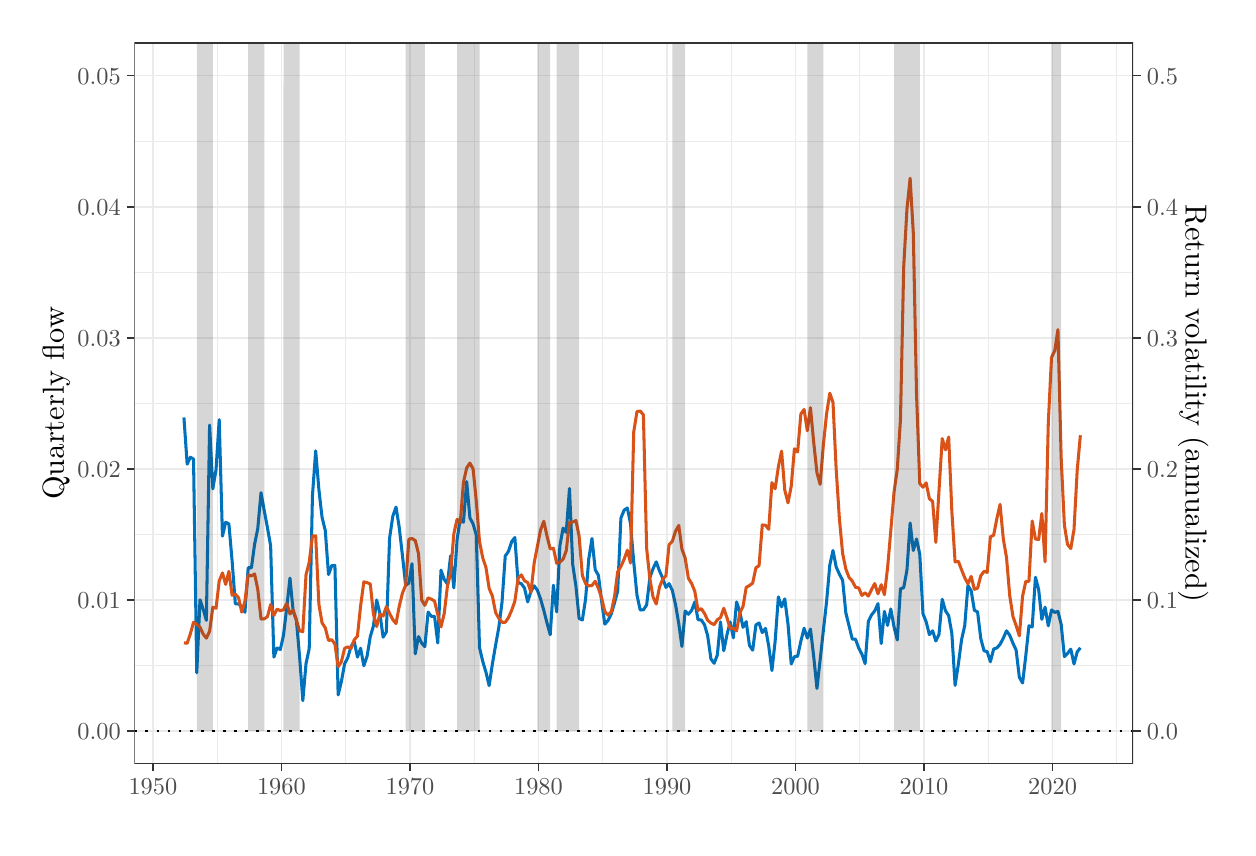
\begin{tikzpicture}[x=1pt,y=1pt]
\definecolor{fillColor}{RGB}{255,255,255}
\path[use as bounding box,fill=fillColor,fill opacity=0.00] (0,0) rectangle (433.62,289.08);
\begin{scope}
\path[clip] (  0.00,  0.00) rectangle (433.62,289.08);
\definecolor{drawColor}{RGB}{255,255,255}
\definecolor{fillColor}{RGB}{255,255,255}

\path[draw=drawColor,line width= 0.6pt,line join=round,line cap=round,fill=fillColor] (  0.00,  0.00) rectangle (433.62,289.08);
\end{scope}
\begin{scope}
\path[clip] ( 38.56, 23.11) rectangle (399.46,283.58);
\definecolor{fillColor}{RGB}{255,255,255}

\path[fill=fillColor] ( 38.56, 23.11) rectangle (399.46,283.58);
\definecolor{drawColor}{gray}{0.92}

\path[draw=drawColor,line width= 0.3pt,line join=round] ( 38.56, 58.63) --
	(399.46, 58.63);

\path[draw=drawColor,line width= 0.3pt,line join=round] ( 38.56,105.99) --
	(399.46,105.99);

\path[draw=drawColor,line width= 0.3pt,line join=round] ( 38.56,153.34) --
	(399.46,153.34);

\path[draw=drawColor,line width= 0.3pt,line join=round] ( 38.56,200.70) --
	(399.46,200.70);

\path[draw=drawColor,line width= 0.3pt,line join=round] ( 38.56,248.06) --
	(399.46,248.06);

\path[draw=drawColor,line width= 0.3pt,line join=round] ( 68.46, 23.11) --
	( 68.46,283.58);

\path[draw=drawColor,line width= 0.3pt,line join=round] (114.91, 23.11) --
	(114.91,283.58);

\path[draw=drawColor,line width= 0.3pt,line join=round] (161.35, 23.11) --
	(161.35,283.58);

\path[draw=drawColor,line width= 0.3pt,line join=round] (207.79, 23.11) --
	(207.79,283.58);

\path[draw=drawColor,line width= 0.3pt,line join=round] (254.24, 23.11) --
	(254.24,283.58);

\path[draw=drawColor,line width= 0.3pt,line join=round] (300.68, 23.11) --
	(300.68,283.58);

\path[draw=drawColor,line width= 0.3pt,line join=round] (347.13, 23.11) --
	(347.13,283.58);

\path[draw=drawColor,line width= 0.3pt,line join=round] (393.57, 23.11) --
	(393.57,283.58);

\path[draw=drawColor,line width= 0.6pt,line join=round] ( 38.56, 34.95) --
	(399.46, 34.95);

\path[draw=drawColor,line width= 0.6pt,line join=round] ( 38.56, 82.31) --
	(399.46, 82.31);

\path[draw=drawColor,line width= 0.6pt,line join=round] ( 38.56,129.67) --
	(399.46,129.67);

\path[draw=drawColor,line width= 0.6pt,line join=round] ( 38.56,177.02) --
	(399.46,177.02);

\path[draw=drawColor,line width= 0.6pt,line join=round] ( 38.56,224.38) --
	(399.46,224.38);

\path[draw=drawColor,line width= 0.6pt,line join=round] ( 38.56,271.74) --
	(399.46,271.74);

\path[draw=drawColor,line width= 0.6pt,line join=round] ( 45.24, 23.11) --
	( 45.24,283.58);

\path[draw=drawColor,line width= 0.6pt,line join=round] ( 91.68, 23.11) --
	( 91.68,283.58);

\path[draw=drawColor,line width= 0.6pt,line join=round] (138.13, 23.11) --
	(138.13,283.58);

\path[draw=drawColor,line width= 0.6pt,line join=round] (184.57, 23.11) --
	(184.57,283.58);

\path[draw=drawColor,line width= 0.6pt,line join=round] (231.02, 23.11) --
	(231.02,283.58);

\path[draw=drawColor,line width= 0.6pt,line join=round] (277.46, 23.11) --
	(277.46,283.58);

\path[draw=drawColor,line width= 0.6pt,line join=round] (323.91, 23.11) --
	(323.91,283.58);

\path[draw=drawColor,line width= 0.6pt,line join=round] (370.35, 23.11) --
	(370.35,283.58);
\definecolor{drawColor}{RGB}{0,114,189}

\path[draw=drawColor,line width= 1.1pt,line join=round] ( 56.46,148.23) --
	( 57.63,131.35) --
	( 58.78,133.87) --
	( 59.93,133.20) --
	( 61.10, 55.94) --
	( 62.27, 82.35) --
	( 63.43, 78.92) --
	( 64.57, 74.89) --
	( 65.74,145.46) --
	( 66.91,122.40) --
	( 68.07,129.42) --
	( 69.21,147.43) --
	( 70.38,105.35) --
	( 71.55,110.38) --
	( 72.71,109.76) --
	( 73.87, 96.40) --
	( 75.04, 80.86) --
	( 76.20, 80.88) --
	( 77.36, 79.88) --
	( 78.51, 77.82) --
	( 79.68, 93.93) --
	( 80.85, 93.90) --
	( 82.00,102.42) --
	( 83.15,108.14) --
	( 84.32,121.04) --
	( 85.49,114.52) --
	( 86.64,108.37) --
	( 87.79,101.91) --
	( 88.96, 61.63) --
	( 90.13, 64.95) --
	( 91.29, 64.36) --
	( 92.44, 69.56) --
	( 93.61, 79.49) --
	( 94.78, 90.18) --
	( 95.94, 78.14) --
	( 97.08, 75.12) --
	( 98.25, 61.92) --
	( 99.42, 45.90) --
	(100.58, 59.30) --
	(101.73, 64.67) --
	(102.90,119.95) --
	(104.07,136.18) --
	(105.22,122.28) --
	(106.37,112.15) --
	(107.54,107.36) --
	(108.71, 91.45) --
	(109.86, 94.67) --
	(111.02, 94.74) --
	(112.19, 47.96) --
	(113.36, 52.82) --
	(114.52, 59.22) --
	(115.66, 61.39) --
	(116.83, 65.47) --
	(118.00, 67.32) --
	(119.16, 61.64) --
	(120.30, 64.84) --
	(121.47, 58.49) --
	(122.64, 61.94) --
	(123.80, 68.99) --
	(124.94, 72.90) --
	(126.11, 82.27) --
	(127.28, 77.37) --
	(128.44, 68.83) --
	(129.60, 70.71) --
	(130.77,104.58) --
	(131.94,112.55) --
	(133.10,115.85) --
	(134.24,108.68) --
	(135.41, 98.46) --
	(136.58, 87.58) --
	(137.74, 88.39) --
	(138.88, 95.39) --
	(140.05, 62.80) --
	(141.22, 69.07) --
	(142.38, 66.67) --
	(143.52, 65.38) --
	(144.69, 77.91) --
	(145.86, 76.38) --
	(147.02, 76.35) --
	(148.18, 66.75) --
	(149.35, 93.06) --
	(150.52, 89.72) --
	(151.67, 88.05) --
	(152.82, 98.25) --
	(153.99, 86.66) --
	(155.16,104.07) --
	(156.31,111.69) --
	(157.46,110.35) --
	(158.63,125.07) --
	(159.80,111.97) --
	(160.96,109.72) --
	(162.10,105.75) --
	(163.27, 65.08) --
	(164.44, 60.06) --
	(165.60, 56.18) --
	(166.75, 51.32) --
	(167.92, 59.16) --
	(169.09, 65.97) --
	(170.25, 72.39) --
	(171.40, 81.43) --
	(172.57, 98.18) --
	(173.73, 99.82) --
	(174.89,103.34) --
	(176.04,104.86) --
	(177.21, 88.53) --
	(178.38, 88.19) --
	(179.53, 86.58) --
	(180.68, 81.58) --
	(181.85, 85.38) --
	(183.02, 87.39) --
	(184.17, 85.81) --
	(185.33, 82.66) --
	(186.50, 78.55) --
	(187.67, 73.90) --
	(188.83, 69.71) --
	(189.97, 87.62) --
	(191.14, 77.98) --
	(192.31,101.82) --
	(193.47,108.25) --
	(194.61,106.69) --
	(195.78,122.58) --
	(196.95, 95.08) --
	(198.11, 87.28) --
	(199.26, 75.61) --
	(200.43, 75.03) --
	(201.60, 82.62) --
	(202.75, 97.16) --
	(203.91,104.49) --
	(205.08, 93.21) --
	(206.25, 91.12) --
	(207.41, 81.73) --
	(208.55, 73.54) --
	(209.72, 74.87) --
	(210.89, 77.29) --
	(212.05, 81.20) --
	(213.19, 85.43) --
	(214.36,111.86) --
	(215.53,114.75) --
	(216.69,115.53) --
	(217.83,109.83) --
	(219.00, 95.94) --
	(220.17, 84.02) --
	(221.33, 78.66) --
	(222.49, 78.71) --
	(223.66, 80.48) --
	(224.83, 90.41) --
	(225.98, 93.59) --
	(227.13, 96.06) --
	(228.30, 92.78) --
	(229.47, 90.17) --
	(230.63, 86.82) --
	(231.77, 88.18) --
	(232.94, 85.72) --
	(234.11, 80.54) --
	(235.27, 73.75) --
	(236.41, 65.47) --
	(237.58, 78.29) --
	(238.75, 77.12) --
	(239.91, 78.51) --
	(241.06, 81.54) --
	(242.23, 75.15) --
	(243.40, 75.05) --
	(244.56, 73.36) --
	(245.71, 69.40) --
	(246.88, 61.00) --
	(248.05, 59.40) --
	(249.20, 62.36) --
	(250.35, 74.36) --
	(251.52, 63.92) --
	(252.69, 69.71) --
	(253.84, 74.34) --
	(254.99, 68.59) --
	(256.16, 81.58) --
	(257.33, 77.98) --
	(258.49, 72.40) --
	(259.64, 74.44) --
	(260.81, 65.85) --
	(261.98, 64.13) --
	(263.14, 73.26) --
	(264.28, 73.98) --
	(265.45, 70.49) --
	(266.62, 72.03) --
	(267.78, 65.60) --
	(268.93, 56.78) --
	(270.10, 67.42) --
	(271.26, 83.40) --
	(272.42, 79.82) --
	(273.57, 82.68) --
	(274.74, 73.61) --
	(275.91, 59.14) --
	(277.06, 61.79) --
	(278.22, 61.96) --
	(279.39, 67.39) --
	(280.56, 72.08) --
	(281.72, 68.52) --
	(282.86, 71.76) --
	(284.03, 61.85) --
	(285.20, 50.31) --
	(286.36, 60.66) --
	(287.50, 71.10) --
	(288.67, 81.53) --
	(289.84, 94.91) --
	(291.00,100.15) --
	(292.14, 94.25) --
	(293.31, 91.60) --
	(294.48, 89.41) --
	(295.64, 77.63) --
	(296.80, 72.95) --
	(297.97, 68.14) --
	(299.14, 68.10) --
	(300.30, 64.88) --
	(301.44, 62.72) --
	(302.61, 59.25) --
	(303.78, 74.55) --
	(304.94, 76.89) --
	(306.08, 78.32) --
	(307.25, 80.95) --
	(308.42, 66.52) --
	(309.58, 78.17) --
	(310.72, 73.09) --
	(311.89, 79.03) --
	(313.06, 72.53) --
	(314.22, 67.82) --
	(315.38, 86.32) --
	(316.55, 86.73) --
	(317.72, 93.05) --
	(318.87,110.10) --
	(320.02,100.16) --
	(321.19,104.32) --
	(322.36, 98.80) --
	(323.51, 77.33) --
	(324.66, 74.39) --
	(325.83, 69.74) --
	(327.00, 71.15) --
	(328.16, 67.46) --
	(329.30, 69.85) --
	(330.47, 82.54) --
	(331.64, 78.38) --
	(332.80, 76.60) --
	(333.95, 70.19) --
	(335.12, 51.40) --
	(336.29, 59.02) --
	(337.45, 67.88) --
	(338.60, 72.98) --
	(339.76, 87.52) --
	(340.93, 85.63) --
	(342.09, 78.53) --
	(343.24, 77.98) --
	(344.41, 68.27) --
	(345.58, 63.96) --
	(346.73, 63.57) --
	(347.88, 59.95) --
	(349.05, 64.56) --
	(350.22, 64.98) --
	(351.37, 66.23) --
	(352.53, 68.46) --
	(353.70, 71.13) --
	(354.87, 69.50) --
	(356.03, 66.65) --
	(357.17, 64.18) --
	(358.34, 54.32) --
	(359.51, 52.28) --
	(360.67, 62.19) --
	(361.81, 72.94) --
	(362.98, 72.51) --
	(364.15, 90.49) --
	(365.31, 86.11) --
	(366.46, 75.25) --
	(367.63, 79.68) --
	(368.80, 72.94) --
	(369.95, 78.69) --
	(371.11, 77.80) --
	(372.28, 78.14) --
	(373.45, 73.51) --
	(374.61, 61.79) --
	(375.75, 62.97) --
	(376.92, 64.51) --
	(378.09, 59.15) --
	(379.25, 63.53) --
	(380.39, 65.00);
\definecolor{drawColor}{RGB}{217,83,25}

\path[draw=drawColor,line width= 1.1pt,line join=round] ( 56.46, 66.79) --
	( 57.63, 66.63) --
	( 58.78, 70.01) --
	( 59.93, 74.24) --
	( 61.10, 73.46) --
	( 62.27, 72.45) --
	( 63.43, 69.92) --
	( 64.57, 68.49) --
	( 65.74, 70.98) --
	( 66.91, 79.67) --
	( 68.07, 79.29) --
	( 69.21, 89.14) --
	( 70.38, 92.05) --
	( 71.55, 87.89) --
	( 72.71, 92.64) --
	( 73.87, 84.00) --
	( 75.04, 84.38) --
	( 76.20, 83.09) --
	( 77.36, 77.90) --
	( 78.51, 81.82) --
	( 79.68, 91.35) --
	( 80.85, 90.96) --
	( 82.00, 91.70) --
	( 83.15, 86.06) --
	( 84.32, 75.39) --
	( 85.49, 75.45) --
	( 86.64, 76.25) --
	( 87.79, 80.63) --
	( 88.96, 76.66) --
	( 90.13, 78.98) --
	( 91.29, 78.40) --
	( 92.44, 78.75) --
	( 93.61, 81.06) --
	( 94.78, 77.21) --
	( 95.94, 78.67) --
	( 97.08, 74.98) --
	( 98.25, 71.08) --
	( 99.42, 70.85) --
	(100.58, 91.38) --
	(101.73, 95.84) --
	(102.90,105.40) --
	(104.07,105.47) --
	(105.22, 80.76) --
	(106.37, 74.04) --
	(107.54, 72.19) --
	(108.71, 67.64) --
	(109.86, 67.92) --
	(111.02, 66.37) --
	(112.19, 58.11) --
	(113.36, 59.95) --
	(114.52, 64.81) --
	(115.66, 65.33) --
	(116.83, 64.75) --
	(118.00, 67.89) --
	(119.16, 69.21) --
	(120.30, 80.08) --
	(121.47, 88.83) --
	(122.64, 88.53) --
	(123.80, 88.06) --
	(124.94, 77.14) --
	(126.11, 72.68) --
	(127.28, 77.15) --
	(128.44, 76.49) --
	(129.60, 79.88) --
	(130.77, 77.45) --
	(131.94, 75.16) --
	(133.10, 73.75) --
	(134.24, 79.88) --
	(135.41, 84.72) --
	(136.58, 87.65) --
	(137.74,104.26) --
	(138.88,104.48) --
	(140.05,103.77) --
	(141.22, 99.06) --
	(142.38, 82.25) --
	(143.52, 80.33) --
	(144.69, 83.03) --
	(145.86, 82.59) --
	(147.02, 81.88) --
	(148.18, 77.04) --
	(149.35, 72.54) --
	(150.52, 77.41) --
	(151.67, 87.21) --
	(152.82, 91.97) --
	(153.99,106.16) --
	(155.16,111.43) --
	(156.31,110.05) --
	(157.46,124.74) --
	(158.63,130.00) --
	(159.80,131.73) --
	(160.96,129.62) --
	(162.10,118.01) --
	(163.27,103.44) --
	(164.44, 97.48) --
	(165.60, 93.99) --
	(166.75, 86.47) --
	(167.92, 83.69) --
	(169.09, 77.73) --
	(170.25, 75.65) --
	(171.40, 74.24) --
	(172.57, 74.19) --
	(173.73, 75.89) --
	(174.89, 78.55) --
	(176.04, 81.81) --
	(177.21, 90.12) --
	(178.38, 91.36) --
	(179.53, 89.21) --
	(180.68, 88.59) --
	(181.85, 85.09) --
	(183.02, 95.64) --
	(184.17,101.64) --
	(185.33,107.56) --
	(186.50,110.74) --
	(187.67,105.31) --
	(188.83,100.72) --
	(189.97,100.99) --
	(191.14, 95.56) --
	(192.31, 95.98) --
	(193.47, 97.02) --
	(194.61,100.06) --
	(195.78,110.33) --
	(196.95,110.46) --
	(198.11,110.97) --
	(199.26,105.40) --
	(200.43, 91.12) --
	(201.60, 88.19) --
	(202.75, 87.35) --
	(203.91, 87.51) --
	(205.08, 89.04) --
	(206.25, 86.42) --
	(207.41, 82.96) --
	(208.55, 78.08) --
	(209.72, 76.80) --
	(210.89, 78.06) --
	(212.05, 83.47) --
	(213.19, 92.44) --
	(214.36, 94.36) --
	(215.53, 97.03) --
	(216.69,100.26) --
	(217.83, 95.62) --
	(219.00,143.01) --
	(220.17,150.37) --
	(221.33,150.55) --
	(222.49,149.16) --
	(223.66,100.92) --
	(224.83, 89.92) --
	(225.98, 83.33) --
	(227.13, 80.82) --
	(228.30, 86.93) --
	(229.47, 89.78) --
	(230.63, 91.01) --
	(231.77,102.25) --
	(232.94,103.50) --
	(234.11,107.13) --
	(235.27,109.20) --
	(236.41,100.63) --
	(237.58, 97.48) --
	(238.75, 90.11) --
	(239.91, 88.22) --
	(241.06, 85.41) --
	(242.23, 78.50) --
	(243.40, 79.15) --
	(244.56, 77.44) --
	(245.71, 74.96) --
	(246.88, 73.94) --
	(248.05, 73.35) --
	(249.20, 75.13) --
	(250.35, 75.89) --
	(251.52, 79.28) --
	(252.69, 75.87) --
	(253.84, 71.99) --
	(254.99, 72.13) --
	(256.16, 71.11) --
	(257.33, 77.64) --
	(258.49, 79.92) --
	(259.64, 86.85) --
	(260.81, 87.49) --
	(261.98, 88.38) --
	(263.14, 93.90) --
	(264.28, 94.67) --
	(265.45,109.38) --
	(266.62,109.28) --
	(267.78,107.81) --
	(268.93,124.69) --
	(270.10,122.46) --
	(271.26,130.41) --
	(272.42,136.06) --
	(273.57,121.99) --
	(274.74,117.36) --
	(275.91,123.39) --
	(277.06,136.92) --
	(278.22,135.75) --
	(279.39,149.50) --
	(280.56,151.12) --
	(281.72,143.42) --
	(282.86,151.77) --
	(284.03,139.22) --
	(285.20,128.25) --
	(286.36,124.05) --
	(287.50,138.10) --
	(288.67,149.44) --
	(289.84,156.99) --
	(291.00,153.66) --
	(292.14,129.69) --
	(293.31,111.68) --
	(294.48, 99.09) --
	(295.64, 93.48) --
	(296.80, 90.43) --
	(297.97, 89.10) --
	(299.14, 86.85) --
	(300.30, 86.64) --
	(301.44, 83.92) --
	(302.61, 84.86) --
	(303.78, 83.68) --
	(304.94, 86.08) --
	(306.08, 88.22) --
	(307.25, 84.50) --
	(308.42, 87.78) --
	(309.58, 84.18) --
	(310.72, 93.87) --
	(311.89,107.32) --
	(313.06,121.37) --
	(314.22,129.43) --
	(315.38,147.40) --
	(316.55,202.67) --
	(317.72,223.49) --
	(318.87,234.68) --
	(320.02,214.83) --
	(321.19,156.57) --
	(322.36,124.36) --
	(323.51,123.02) --
	(324.66,124.58) --
	(325.83,118.87) --
	(327.00,117.90) --
	(328.16,103.08) --
	(329.30,121.67) --
	(330.47,140.60) --
	(331.64,136.53) --
	(332.80,141.16) --
	(333.95,114.22) --
	(335.12, 96.02) --
	(336.29, 96.26) --
	(337.45, 93.20) --
	(338.60, 90.33) --
	(339.76, 88.12) --
	(340.93, 90.80) --
	(342.09, 86.12) --
	(343.24, 86.53) --
	(344.41, 91.01) --
	(345.58, 92.63) --
	(346.73, 92.25) --
	(347.88,105.13) --
	(349.05,105.65) --
	(350.22,111.74) --
	(351.37,116.80) --
	(352.53,104.47) --
	(353.70, 97.60) --
	(354.87, 83.78) --
	(356.03, 76.28) --
	(357.17, 73.03) --
	(358.34, 69.30) --
	(359.51, 83.68) --
	(360.67, 89.00) --
	(361.81, 89.02) --
	(362.98,110.84) --
	(364.15,104.33) --
	(365.31,104.12) --
	(366.46,113.54) --
	(367.63, 96.07) --
	(368.80,146.28) --
	(369.95,169.89) --
	(371.11,172.32) --
	(372.28,179.97) --
	(373.45,133.71) --
	(374.61,109.32) --
	(375.75,102.33) --
	(376.92,100.85) --
	(378.09,107.76) --
	(379.25,129.21) --
	(380.39,141.80);
\definecolor{fillColor}{RGB}{51,51,51}

\path[fill=fillColor,fill opacity=0.20] ( 55.29, 34.95) --
	( 55.61, 34.95) --
	( 56.13, 34.95) --
	( 56.46, 34.95) --
	( 56.78, 34.95) --
	( 57.30, 34.95) --
	( 57.63, 34.95) --
	( 57.95, 34.95) --
	( 58.46, 34.95) --
	( 58.78, 34.95) --
	( 59.11, 34.95) --
	( 59.60, 34.95) --
	( 59.93, 34.95) --
	( 60.26, 34.95) --
	( 60.77, 34.95) --
	( 61.10, 34.95) --
	( 61.10,2023.56) --
	( 66.90,2023.56) --
	( 66.91, 34.95) --
	( 67.24, 34.95) --
	( 67.74, 34.95) --
	( 68.07, 34.95) --
	( 68.39, 34.95) --
	( 68.88, 34.95) --
	( 69.21, 34.95) --
	( 69.54, 34.95) --
	( 70.05, 34.95) --
	( 70.38, 34.95) --
	( 70.71, 34.95) --
	( 71.22, 34.95) --
	( 71.55, 34.95) --
	( 71.88, 34.95) --
	( 72.38, 34.95) --
	( 72.71, 34.95) --
	( 73.04, 34.95) --
	( 73.54, 34.95) --
	( 73.87, 34.95) --
	( 74.19, 34.95) --
	( 74.71, 34.95) --
	( 75.04, 34.95) --
	( 75.36, 34.95) --
	( 75.88, 34.95) --
	( 76.20, 34.95) --
	( 76.53, 34.95) --
	( 77.03, 34.95) --
	( 77.36, 34.95) --
	( 77.69, 34.95) --
	( 78.18, 34.95) --
	( 78.51, 34.95) --
	( 78.83, 34.95) --
	( 79.35, 34.95) --
	( 79.68, 34.95) --
	( 79.68,2023.56) --
	( 85.48,2023.56) --
	( 85.49, 34.95) --
	( 85.81, 34.95) --
	( 86.32, 34.95) --
	( 86.64, 34.95) --
	( 86.97, 34.95) --
	( 87.46, 34.95) --
	( 87.79, 34.95) --
	( 88.12, 34.95) --
	( 88.63, 34.95) --
	( 88.96, 34.95) --
	( 89.29, 34.95) --
	( 89.80, 34.95) --
	( 90.13, 34.95) --
	( 90.46, 34.95) --
	( 90.96, 34.95) --
	( 91.29, 34.95) --
	( 91.61, 34.95) --
	( 92.12, 34.95) --
	( 92.44, 34.95) --
	( 92.45,2023.56) --
	( 98.25,2023.56) --
	( 98.25, 34.95) --
	( 98.58, 34.95) --
	( 99.10, 34.95) --
	( 99.42, 34.95) --
	( 99.75, 34.95) --
	(100.25, 34.95) --
	(100.58, 34.95) --
	(100.91, 34.95) --
	(101.40, 34.95) --
	(101.73, 34.95) --
	(102.05, 34.95) --
	(102.57, 34.95) --
	(102.90, 34.95) --
	(103.22, 34.95) --
	(103.74, 34.95) --
	(104.07, 34.95) --
	(104.39, 34.95) --
	(104.89, 34.95) --
	(105.22, 34.95) --
	(105.55, 34.95) --
	(106.04, 34.95) --
	(106.37, 34.95) --
	(106.69, 34.95) --
	(107.21, 34.95) --
	(107.54, 34.95) --
	(107.86, 34.95) --
	(108.38, 34.95) --
	(108.71, 34.95) --
	(109.03, 34.95) --
	(109.54, 34.95) --
	(109.86, 34.95) --
	(110.19, 34.95) --
	(110.69, 34.95) --
	(111.02, 34.95) --
	(111.35, 34.95) --
	(111.86, 34.95) --
	(112.19, 34.95) --
	(112.52, 34.95) --
	(113.03, 34.95) --
	(113.36, 34.95) --
	(113.69, 34.95) --
	(114.19, 34.95) --
	(114.52, 34.95) --
	(114.84, 34.95) --
	(115.33, 34.95) --
	(115.66, 34.95) --
	(115.99, 34.95) --
	(116.50, 34.95) --
	(116.83, 34.95) --
	(117.16, 34.95) --
	(117.67, 34.95) --
	(118.00, 34.95) --
	(118.33, 34.95) --
	(118.83, 34.95) --
	(119.16, 34.95) --
	(119.49, 34.95) --
	(119.98, 34.95) --
	(120.30, 34.95) --
	(120.63, 34.95) --
	(121.15, 34.95) --
	(121.47, 34.95) --
	(121.80, 34.95) --
	(122.32, 34.95) --
	(122.64, 34.95) --
	(122.97, 34.95) --
	(123.47, 34.95) --
	(123.80, 34.95) --
	(124.13, 34.95) --
	(124.62, 34.95) --
	(124.94, 34.95) --
	(125.27, 34.95) --
	(125.79, 34.95) --
	(126.11, 34.95) --
	(126.44, 34.95) --
	(126.96, 34.95) --
	(127.28, 34.95) --
	(127.61, 34.95) --
	(128.11, 34.95) --
	(128.44, 34.95) --
	(128.77, 34.95) --
	(129.27, 34.95) --
	(129.60, 34.95) --
	(129.93, 34.95) --
	(130.44, 34.95) --
	(130.77, 34.95) --
	(131.10, 34.95) --
	(131.61, 34.95) --
	(131.94, 34.95) --
	(132.27, 34.95) --
	(132.77, 34.95) --
	(133.10, 34.95) --
	(133.42, 34.95) --
	(133.91, 34.95) --
	(134.24, 34.95) --
	(134.57, 34.95) --
	(135.08, 34.95) --
	(135.41, 34.95) --
	(135.74, 34.95) --
	(136.25, 34.95) --
	(136.58, 34.95) --
	(136.58,2023.56) --
	(143.52,2023.56) --
	(143.52, 34.95) --
	(143.85, 34.95) --
	(144.36, 34.95) --
	(144.69, 34.95) --
	(145.02, 34.95) --
	(145.53, 34.95) --
	(145.86, 34.95) --
	(146.19, 34.95) --
	(146.69, 34.95) --
	(147.02, 34.95) --
	(147.35, 34.95) --
	(147.85, 34.95) --
	(148.18, 34.95) --
	(148.50, 34.95) --
	(149.02, 34.95) --
	(149.35, 34.95) --
	(149.67, 34.95) --
	(150.19, 34.95) --
	(150.52, 34.95) --
	(150.84, 34.95) --
	(151.35, 34.95) --
	(151.67, 34.95) --
	(152.00, 34.95) --
	(152.49, 34.95) --
	(152.82, 34.95) --
	(153.14, 34.95) --
	(153.66, 34.95) --
	(153.99, 34.95) --
	(154.31, 34.95) --
	(154.83, 34.95) --
	(155.16, 34.95) --
	(155.16,2023.56) --
	(163.26,2023.56) --
	(163.27, 34.95) --
	(163.60, 34.95) --
	(164.11, 34.95) --
	(164.44, 34.95) --
	(164.77, 34.95) --
	(165.27, 34.95) --
	(165.60, 34.95) --
	(165.92, 34.95) --
	(166.43, 34.95) --
	(166.75, 34.95) --
	(167.08, 34.95) --
	(167.60, 34.95) --
	(167.92, 34.95) --
	(168.25, 34.95) --
	(168.77, 34.95) --
	(169.09, 34.95) --
	(169.42, 34.95) --
	(169.92, 34.95) --
	(170.25, 34.95) --
	(170.58, 34.95) --
	(171.07, 34.95) --
	(171.40, 34.95) --
	(171.72, 34.95) --
	(172.24, 34.95) --
	(172.57, 34.95) --
	(172.89, 34.95) --
	(173.41, 34.95) --
	(173.73, 34.95) --
	(174.06, 34.95) --
	(174.56, 34.95) --
	(174.89, 34.95) --
	(175.22, 34.95) --
	(175.71, 34.95) --
	(176.04, 34.95) --
	(176.36, 34.95) --
	(176.88, 34.95) --
	(177.21, 34.95) --
	(177.53, 34.95) --
	(178.05, 34.95) --
	(178.38, 34.95) --
	(178.70, 34.95) --
	(179.21, 34.95) --
	(179.53, 34.95) --
	(179.86, 34.95) --
	(180.35, 34.95) --
	(180.68, 34.95) --
	(181.01, 34.95) --
	(181.52, 34.95) --
	(181.85, 34.95) --
	(182.18, 34.95) --
	(182.69, 34.95) --
	(183.02, 34.95) --
	(183.34, 34.95) --
	(183.85, 34.95) --
	(184.17, 34.95) --
	(184.18,2023.56) --
	(188.82,2023.56) --
	(188.83, 34.95) --
	(189.16, 34.95) --
	(189.65, 34.95) --
	(189.97, 34.95) --
	(190.30, 34.95) --
	(190.82, 34.95) --
	(191.14, 34.95) --
	(191.15,2023.56) --
	(199.25,2023.56) --
	(199.26, 34.95) --
	(199.58, 34.95) --
	(200.10, 34.95) --
	(200.43, 34.95) --
	(200.75, 34.95) --
	(201.27, 34.95) --
	(201.60, 34.95) --
	(201.92, 34.95) --
	(202.42, 34.95) --
	(202.75, 34.95) --
	(203.08, 34.95) --
	(203.58, 34.95) --
	(203.91, 34.95) --
	(204.24, 34.95) --
	(204.75, 34.95) --
	(205.08, 34.95) --
	(205.41, 34.95) --
	(205.92, 34.95) --
	(206.25, 34.95) --
	(206.58, 34.95) --
	(207.08, 34.95) --
	(207.41, 34.95) --
	(207.73, 34.95) --
	(208.22, 34.95) --
	(208.55, 34.95) --
	(208.88, 34.95) --
	(209.39, 34.95) --
	(209.72, 34.95) --
	(210.05, 34.95) --
	(210.56, 34.95) --
	(210.89, 34.95) --
	(211.22, 34.95) --
	(211.72, 34.95) --
	(212.05, 34.95) --
	(212.38, 34.95) --
	(212.86, 34.95) --
	(213.19, 34.95) --
	(213.52, 34.95) --
	(214.03, 34.95) --
	(214.36, 34.95) --
	(214.69, 34.95) --
	(215.20, 34.95) --
	(215.53, 34.95) --
	(215.86, 34.95) --
	(216.36, 34.95) --
	(216.69, 34.95) --
	(217.02, 34.95) --
	(217.51, 34.95) --
	(217.83, 34.95) --
	(218.16, 34.95) --
	(218.68, 34.95) --
	(219.00, 34.95) --
	(219.33, 34.95) --
	(219.85, 34.95) --
	(220.17, 34.95) --
	(220.50, 34.95) --
	(221.00, 34.95) --
	(221.33, 34.95) --
	(221.66, 34.95) --
	(222.16, 34.95) --
	(222.49, 34.95) --
	(222.81, 34.95) --
	(223.33, 34.95) --
	(223.66, 34.95) --
	(223.98, 34.95) --
	(224.50, 34.95) --
	(224.83, 34.95) --
	(225.15, 34.95) --
	(225.66, 34.95) --
	(225.98, 34.95) --
	(226.31, 34.95) --
	(226.80, 34.95) --
	(227.13, 34.95) --
	(227.46, 34.95) --
	(227.97, 34.95) --
	(228.30, 34.95) --
	(228.63, 34.95) --
	(229.14, 34.95) --
	(229.47, 34.95) --
	(229.80, 34.95) --
	(230.30, 34.95) --
	(230.63, 34.95) --
	(230.95, 34.95) --
	(231.44, 34.95) --
	(231.77, 34.95) --
	(232.10, 34.95) --
	(232.61, 34.95) --
	(232.94, 34.95) --
	(232.94,2023.56) --
	(237.58,2023.56) --
	(237.58, 34.95) --
	(237.91, 34.95) --
	(238.42, 34.95) --
	(238.75, 34.95) --
	(239.08, 34.95) --
	(239.58, 34.95) --
	(239.91, 34.95) --
	(240.24, 34.95) --
	(240.74, 34.95) --
	(241.06, 34.95) --
	(241.39, 34.95) --
	(241.91, 34.95) --
	(242.23, 34.95) --
	(242.56, 34.95) --
	(243.08, 34.95) --
	(243.40, 34.95) --
	(243.73, 34.95) --
	(244.23, 34.95) --
	(244.56, 34.95) --
	(244.89, 34.95) --
	(245.38, 34.95) --
	(245.71, 34.95) --
	(246.03, 34.95) --
	(246.55, 34.95) --
	(246.88, 34.95) --
	(247.20, 34.95) --
	(247.72, 34.95) --
	(248.05, 34.95) --
	(248.37, 34.95) --
	(248.88, 34.95) --
	(249.20, 34.95) --
	(249.53, 34.95) --
	(250.02, 34.95) --
	(250.35, 34.95) --
	(250.67, 34.95) --
	(251.19, 34.95) --
	(251.52, 34.95) --
	(251.84, 34.95) --
	(252.36, 34.95) --
	(252.69, 34.95) --
	(253.01, 34.95) --
	(253.52, 34.95) --
	(253.84, 34.95) --
	(254.17, 34.95) --
	(254.66, 34.95) --
	(254.99, 34.95) --
	(255.32, 34.95) --
	(255.83, 34.95) --
	(256.16, 34.95) --
	(256.49, 34.95) --
	(257.00, 34.95) --
	(257.33, 34.95) --
	(257.66, 34.95) --
	(258.16, 34.95) --
	(258.49, 34.95) --
	(258.81, 34.95) --
	(259.32, 34.95) --
	(259.64, 34.95) --
	(259.97, 34.95) --
	(260.49, 34.95) --
	(260.81, 34.95) --
	(261.14, 34.95) --
	(261.66, 34.95) --
	(261.98, 34.95) --
	(262.31, 34.95) --
	(262.81, 34.95) --
	(263.14, 34.95) --
	(263.47, 34.95) --
	(263.96, 34.95) --
	(264.28, 34.95) --
	(264.61, 34.95) --
	(265.13, 34.95) --
	(265.45, 34.95) --
	(265.78, 34.95) --
	(266.30, 34.95) --
	(266.62, 34.95) --
	(266.95, 34.95) --
	(267.45, 34.95) --
	(267.78, 34.95) --
	(268.11, 34.95) --
	(268.60, 34.95) --
	(268.93, 34.95) --
	(269.25, 34.95) --
	(269.77, 34.95) --
	(270.10, 34.95) --
	(270.42, 34.95) --
	(270.94, 34.95) --
	(271.26, 34.95) --
	(271.59, 34.95) --
	(272.09, 34.95) --
	(272.42, 34.95) --
	(272.75, 34.95) --
	(273.24, 34.95) --
	(273.57, 34.95) --
	(273.89, 34.95) --
	(274.41, 34.95) --
	(274.74, 34.95) --
	(275.06, 34.95) --
	(275.58, 34.95) --
	(275.91, 34.95) --
	(276.23, 34.95) --
	(276.74, 34.95) --
	(277.06, 34.95) --
	(277.39, 34.95) --
	(277.89, 34.95) --
	(278.22, 34.95) --
	(278.55, 34.95) --
	(279.06, 34.95) --
	(279.39, 34.95) --
	(279.72, 34.95) --
	(280.23, 34.95) --
	(280.56, 34.95) --
	(280.89, 34.95) --
	(281.39, 34.95) --
	(281.72, 34.95) --
	(281.72,2023.56) --
	(287.50,2023.56) --
	(287.50, 34.95) --
	(287.83, 34.95) --
	(288.35, 34.95) --
	(288.67, 34.95) --
	(289.00, 34.95) --
	(289.52, 34.95) --
	(289.84, 34.95) --
	(290.17, 34.95) --
	(290.67, 34.95) --
	(291.00, 34.95) --
	(291.33, 34.95) --
	(291.82, 34.95) --
	(292.14, 34.95) --
	(292.47, 34.95) --
	(292.99, 34.95) --
	(293.31, 34.95) --
	(293.64, 34.95) --
	(294.16, 34.95) --
	(294.48, 34.95) --
	(294.81, 34.95) --
	(295.31, 34.95) --
	(295.64, 34.95) --
	(295.97, 34.95) --
	(296.47, 34.95) --
	(296.80, 34.95) --
	(297.13, 34.95) --
	(297.64, 34.95) --
	(297.97, 34.95) --
	(298.30, 34.95) --
	(298.81, 34.95) --
	(299.14, 34.95) --
	(299.47, 34.95) --
	(299.97, 34.95) --
	(300.30, 34.95) --
	(300.62, 34.95) --
	(301.11, 34.95) --
	(301.44, 34.95) --
	(301.77, 34.95) --
	(302.28, 34.95) --
	(302.61, 34.95) --
	(302.94, 34.95) --
	(303.45, 34.95) --
	(303.78, 34.95) --
	(304.11, 34.95) --
	(304.61, 34.95) --
	(304.94, 34.95) --
	(305.26, 34.95) --
	(305.75, 34.95) --
	(306.08, 34.95) --
	(306.41, 34.95) --
	(306.92, 34.95) --
	(307.25, 34.95) --
	(307.58, 34.95) --
	(308.09, 34.95) --
	(308.42, 34.95) --
	(308.75, 34.95) --
	(309.25, 34.95) --
	(309.58, 34.95) --
	(309.91, 34.95) --
	(310.39, 34.95) --
	(310.72, 34.95) --
	(311.05, 34.95) --
	(311.56, 34.95) --
	(311.89, 34.95) --
	(312.22, 34.95) --
	(312.73, 34.95) --
	(313.06, 34.95) --
	(313.07,2023.56) --
	(322.35,2023.56) --
	(322.36, 34.95) --
	(322.68, 34.95) --
	(323.19, 34.95) --
	(323.51, 34.95) --
	(323.84, 34.95) --
	(324.33, 34.95) --
	(324.66, 34.95) --
	(324.99, 34.95) --
	(325.50, 34.95) --
	(325.83, 34.95) --
	(326.16, 34.95) --
	(326.67, 34.95) --
	(327.00, 34.95) --
	(327.33, 34.95) --
	(327.83, 34.95) --
	(328.16, 34.95) --
	(328.48, 34.95) --
	(328.97, 34.95) --
	(329.30, 34.95) --
	(329.63, 34.95) --
	(330.14, 34.95) --
	(330.47, 34.95) --
	(330.80, 34.95) --
	(331.31, 34.95) --
	(331.64, 34.95) --
	(331.97, 34.95) --
	(332.47, 34.95) --
	(332.80, 34.95) --
	(333.12, 34.95) --
	(333.63, 34.95) --
	(333.95, 34.95) --
	(334.28, 34.95) --
	(334.80, 34.95) --
	(335.12, 34.95) --
	(335.45, 34.95) --
	(335.97, 34.95) --
	(336.29, 34.95) --
	(336.62, 34.95) --
	(337.12, 34.95) --
	(337.45, 34.95) --
	(337.78, 34.95) --
	(338.27, 34.95) --
	(338.60, 34.95) --
	(338.92, 34.95) --
	(339.44, 34.95) --
	(339.76, 34.95) --
	(340.09, 34.95) --
	(340.61, 34.95) --
	(340.93, 34.95) --
	(341.26, 34.95) --
	(341.76, 34.95) --
	(342.09, 34.95) --
	(342.42, 34.95) --
	(342.91, 34.95) --
	(343.24, 34.95) --
	(343.56, 34.95) --
	(344.08, 34.95) --
	(344.41, 34.95) --
	(344.73, 34.95) --
	(345.25, 34.95) --
	(345.58, 34.95) --
	(345.90, 34.95) --
	(346.41, 34.95) --
	(346.73, 34.95) --
	(347.06, 34.95) --
	(347.55, 34.95) --
	(347.88, 34.95) --
	(348.21, 34.95) --
	(348.72, 34.95) --
	(349.05, 34.95) --
	(349.37, 34.95) --
	(349.89, 34.95) --
	(350.22, 34.95) --
	(350.54, 34.95) --
	(351.05, 34.95) --
	(351.37, 34.95) --
	(351.70, 34.95) --
	(352.20, 34.95) --
	(352.53, 34.95) --
	(352.86, 34.95) --
	(353.37, 34.95) --
	(353.70, 34.95) --
	(354.03, 34.95) --
	(354.54, 34.95) --
	(354.87, 34.95) --
	(355.20, 34.95) --
	(355.70, 34.95) --
	(356.03, 34.95) --
	(356.36, 34.95) --
	(356.85, 34.95) --
	(357.17, 34.95) --
	(357.50, 34.95) --
	(358.02, 34.95) --
	(358.34, 34.95) --
	(358.67, 34.95) --
	(359.19, 34.95) --
	(359.51, 34.95) --
	(359.84, 34.95) --
	(360.34, 34.95) --
	(360.67, 34.95) --
	(361.00, 34.95) --
	(361.49, 34.95) --
	(361.81, 34.95) --
	(362.14, 34.95) --
	(362.66, 34.95) --
	(362.98, 34.95) --
	(363.31, 34.95) --
	(363.83, 34.95) --
	(364.15, 34.95) --
	(364.48, 34.95) --
	(364.98, 34.95) --
	(365.31, 34.95) --
	(365.64, 34.95) --
	(366.13, 34.95) --
	(366.46, 34.95) --
	(366.78, 34.95) --
	(367.30, 34.95) --
	(367.63, 34.95) --
	(367.95, 34.95) --
	(368.47, 34.95) --
	(368.80, 34.95) --
	(369.12, 34.95) --
	(369.62, 34.95) --
	(369.95, 34.95) --
	(369.96,2023.56) --
	(373.44,2023.56) --
	(373.45, 34.95) --
	(373.78, 34.95) --
	(374.28, 34.95) --
	(374.61, 34.95) --
	(374.93, 34.95) --
	(375.42, 34.95) --
	(375.75, 34.95) --
	(376.08, 34.95) --
	(376.59, 34.95) --
	(376.92, 34.95) --
	(377.25, 34.95) --
	(377.76, 34.95) --
	(378.09, 34.95) --
	(378.42, 34.95) --
	(378.92, 34.95) --
	(379.25, 34.95) --
	(379.57, 34.95) --
	(380.06, 34.95) --
	(380.39, 34.95) --
	(380.72, 34.95) --
	(381.23, 34.95) --
	(381.56, 34.95) --
	(381.89, 34.95) --
	(382.40, 34.95) --
	(382.73, 34.95) --
	(383.06, 34.95) --
	(382.73, 34.95) --
	(382.40, 34.95) --
	(381.89, 34.95) --
	(381.56, 34.95) --
	(381.23, 34.95) --
	(380.72, 34.95) --
	(380.39, 34.95) --
	(380.06, 34.95) --
	(379.57, 34.95) --
	(379.25, 34.95) --
	(378.92, 34.95) --
	(378.42, 34.95) --
	(378.09, 34.95) --
	(377.76, 34.95) --
	(377.25, 34.95) --
	(376.92, 34.95) --
	(376.59, 34.95) --
	(376.08, 34.95) --
	(375.75, 34.95) --
	(375.42, 34.95) --
	(374.93, 34.95) --
	(374.61, 34.95) --
	(374.28, 34.95) --
	(373.78, 34.95) --
	(373.45, 34.95) --
	(373.12, 34.95) --
	(372.61, 34.95) --
	(372.28, 34.95) --
	(371.95, 34.95) --
	(371.44, 34.95) --
	(371.11, 34.95) --
	(370.78, 34.95) --
	(370.28, 34.95) --
	(369.95, 34.95) --
	(369.62, 34.95) --
	(369.12, 34.95) --
	(368.80, 34.95) --
	(368.47, 34.95) --
	(367.95, 34.95) --
	(367.63, 34.95) --
	(367.30, 34.95) --
	(366.78, 34.95) --
	(366.46, 34.95) --
	(366.13, 34.95) --
	(365.64, 34.95) --
	(365.31, 34.95) --
	(364.98, 34.95) --
	(364.48, 34.95) --
	(364.15, 34.95) --
	(363.83, 34.95) --
	(363.31, 34.95) --
	(362.98, 34.95) --
	(362.66, 34.95) --
	(362.14, 34.95) --
	(361.81, 34.95) --
	(361.49, 34.95) --
	(361.00, 34.95) --
	(360.67, 34.95) --
	(360.34, 34.95) --
	(359.84, 34.95) --
	(359.51, 34.95) --
	(359.19, 34.95) --
	(358.67, 34.95) --
	(358.34, 34.95) --
	(358.02, 34.95) --
	(357.50, 34.95) --
	(357.17, 34.95) --
	(356.85, 34.95) --
	(356.36, 34.95) --
	(356.03, 34.95) --
	(355.70, 34.95) --
	(355.20, 34.95) --
	(354.87, 34.95) --
	(354.54, 34.95) --
	(354.03, 34.95) --
	(353.70, 34.95) --
	(353.37, 34.95) --
	(352.86, 34.95) --
	(352.53, 34.95) --
	(352.20, 34.95) --
	(351.70, 34.95) --
	(351.37, 34.95) --
	(351.05, 34.95) --
	(350.54, 34.95) --
	(350.22, 34.95) --
	(349.89, 34.95) --
	(349.37, 34.95) --
	(349.05, 34.95) --
	(348.72, 34.95) --
	(348.21, 34.95) --
	(347.88, 34.95) --
	(347.55, 34.95) --
	(347.06, 34.95) --
	(346.73, 34.95) --
	(346.41, 34.95) --
	(345.90, 34.95) --
	(345.58, 34.95) --
	(345.25, 34.95) --
	(344.73, 34.95) --
	(344.41, 34.95) --
	(344.08, 34.95) --
	(343.56, 34.95) --
	(343.24, 34.95) --
	(342.91, 34.95) --
	(342.42, 34.95) --
	(342.09, 34.95) --
	(341.76, 34.95) --
	(341.26, 34.95) --
	(340.93, 34.95) --
	(340.61, 34.95) --
	(340.09, 34.95) --
	(339.76, 34.95) --
	(339.44, 34.95) --
	(338.92, 34.95) --
	(338.60, 34.95) --
	(338.27, 34.95) --
	(337.78, 34.95) --
	(337.45, 34.95) --
	(337.12, 34.95) --
	(336.62, 34.95) --
	(336.29, 34.95) --
	(335.97, 34.95) --
	(335.45, 34.95) --
	(335.12, 34.95) --
	(334.80, 34.95) --
	(334.28, 34.95) --
	(333.95, 34.95) --
	(333.63, 34.95) --
	(333.12, 34.95) --
	(332.80, 34.95) --
	(332.47, 34.95) --
	(331.97, 34.95) --
	(331.64, 34.95) --
	(331.31, 34.95) --
	(330.80, 34.95) --
	(330.47, 34.95) --
	(330.14, 34.95) --
	(329.63, 34.95) --
	(329.30, 34.95) --
	(328.97, 34.95) --
	(328.48, 34.95) --
	(328.16, 34.95) --
	(327.83, 34.95) --
	(327.33, 34.95) --
	(327.00, 34.95) --
	(326.67, 34.95) --
	(326.16, 34.95) --
	(325.83, 34.95) --
	(325.50, 34.95) --
	(324.99, 34.95) --
	(324.66, 34.95) --
	(324.33, 34.95) --
	(323.84, 34.95) --
	(323.51, 34.95) --
	(323.19, 34.95) --
	(322.68, 34.95) --
	(322.36, 34.95) --
	(322.03, 34.95) --
	(321.51, 34.95) --
	(321.19, 34.95) --
	(320.86, 34.95) --
	(320.34, 34.95) --
	(320.02, 34.95) --
	(319.69, 34.95) --
	(319.20, 34.95) --
	(318.87, 34.95) --
	(318.55, 34.95) --
	(318.04, 34.95) --
	(317.72, 34.95) --
	(317.39, 34.95) --
	(316.87, 34.95) --
	(316.55, 34.95) --
	(316.22, 34.95) --
	(315.70, 34.95) --
	(315.38, 34.95) --
	(315.05, 34.95) --
	(314.55, 34.95) --
	(314.22, 34.95) --
	(313.89, 34.95) --
	(313.39, 34.95) --
	(313.06, 34.95) --
	(312.73, 34.95) --
	(312.22, 34.95) --
	(311.89, 34.95) --
	(311.56, 34.95) --
	(311.05, 34.95) --
	(310.72, 34.95) --
	(310.39, 34.95) --
	(309.91, 34.95) --
	(309.58, 34.95) --
	(309.25, 34.95) --
	(308.75, 34.95) --
	(308.42, 34.95) --
	(308.09, 34.95) --
	(307.58, 34.95) --
	(307.25, 34.95) --
	(306.92, 34.95) --
	(306.41, 34.95) --
	(306.08, 34.95) --
	(305.75, 34.95) --
	(305.26, 34.95) --
	(304.94, 34.95) --
	(304.61, 34.95) --
	(304.11, 34.95) --
	(303.78, 34.95) --
	(303.45, 34.95) --
	(302.94, 34.95) --
	(302.61, 34.95) --
	(302.28, 34.95) --
	(301.77, 34.95) --
	(301.44, 34.95) --
	(301.11, 34.95) --
	(300.62, 34.95) --
	(300.30, 34.95) --
	(299.97, 34.95) --
	(299.47, 34.95) --
	(299.14, 34.95) --
	(298.81, 34.95) --
	(298.30, 34.95) --
	(297.97, 34.95) --
	(297.64, 34.95) --
	(297.13, 34.95) --
	(296.80, 34.95) --
	(296.47, 34.95) --
	(295.97, 34.95) --
	(295.64, 34.95) --
	(295.31, 34.95) --
	(294.81, 34.95) --
	(294.48, 34.95) --
	(294.16, 34.95) --
	(293.64, 34.95) --
	(293.31, 34.95) --
	(292.99, 34.95) --
	(292.47, 34.95) --
	(292.14, 34.95) --
	(291.82, 34.95) --
	(291.33, 34.95) --
	(291.00, 34.95) --
	(290.67, 34.95) --
	(290.17, 34.95) --
	(289.84, 34.95) --
	(289.52, 34.95) --
	(289.00, 34.95) --
	(288.67, 34.95) --
	(288.35, 34.95) --
	(287.83, 34.95) --
	(287.50, 34.95) --
	(287.18, 34.95) --
	(286.69, 34.95) --
	(286.36, 34.95) --
	(286.03, 34.95) --
	(285.53, 34.95) --
	(285.20, 34.95) --
	(284.87, 34.95) --
	(284.36, 34.95) --
	(284.03, 34.95) --
	(283.70, 34.95) --
	(283.19, 34.95) --
	(282.86, 34.95) --
	(282.53, 34.95) --
	(282.04, 34.95) --
	(281.72, 34.95) --
	(281.39, 34.95) --
	(280.89, 34.95) --
	(280.56, 34.95) --
	(280.23, 34.95) --
	(279.72, 34.95) --
	(279.39, 34.95) --
	(279.06, 34.95) --
	(278.55, 34.95) --
	(278.22, 34.95) --
	(277.89, 34.95) --
	(277.39, 34.95) --
	(277.06, 34.95) --
	(276.74, 34.95) --
	(276.23, 34.95) --
	(275.91, 34.95) --
	(275.58, 34.95) --
	(275.06, 34.95) --
	(274.74, 34.95) --
	(274.41, 34.95) --
	(273.89, 34.95) --
	(273.57, 34.95) --
	(273.24, 34.95) --
	(272.75, 34.95) --
	(272.42, 34.95) --
	(272.09, 34.95) --
	(271.59, 34.95) --
	(271.26, 34.95) --
	(270.94, 34.95) --
	(270.42, 34.95) --
	(270.10, 34.95) --
	(269.77, 34.95) --
	(269.25, 34.95) --
	(268.93, 34.95) --
	(268.60, 34.95) --
	(268.11, 34.95) --
	(267.78, 34.95) --
	(267.45, 34.95) --
	(266.95, 34.95) --
	(266.62, 34.95) --
	(266.30, 34.95) --
	(265.78, 34.95) --
	(265.45, 34.95) --
	(265.13, 34.95) --
	(264.61, 34.95) --
	(264.28, 34.95) --
	(263.96, 34.95) --
	(263.47, 34.95) --
	(263.14, 34.95) --
	(262.81, 34.95) --
	(262.31, 34.95) --
	(261.98, 34.95) --
	(261.66, 34.95) --
	(261.14, 34.95) --
	(260.81, 34.95) --
	(260.49, 34.95) --
	(259.97, 34.95) --
	(259.64, 34.95) --
	(259.32, 34.95) --
	(258.81, 34.95) --
	(258.49, 34.95) --
	(258.16, 34.95) --
	(257.66, 34.95) --
	(257.33, 34.95) --
	(257.00, 34.95) --
	(256.49, 34.95) --
	(256.16, 34.95) --
	(255.83, 34.95) --
	(255.32, 34.95) --
	(254.99, 34.95) --
	(254.66, 34.95) --
	(254.17, 34.95) --
	(253.84, 34.95) --
	(253.52, 34.95) --
	(253.01, 34.95) --
	(252.69, 34.95) --
	(252.36, 34.95) --
	(251.84, 34.95) --
	(251.52, 34.95) --
	(251.19, 34.95) --
	(250.67, 34.95) --
	(250.35, 34.95) --
	(250.02, 34.95) --
	(249.53, 34.95) --
	(249.20, 34.95) --
	(248.88, 34.95) --
	(248.37, 34.95) --
	(248.05, 34.95) --
	(247.72, 34.95) --
	(247.20, 34.95) --
	(246.88, 34.95) --
	(246.55, 34.95) --
	(246.03, 34.95) --
	(245.71, 34.95) --
	(245.38, 34.95) --
	(244.89, 34.95) --
	(244.56, 34.95) --
	(244.23, 34.95) --
	(243.73, 34.95) --
	(243.40, 34.95) --
	(243.08, 34.95) --
	(242.56, 34.95) --
	(242.23, 34.95) --
	(241.91, 34.95) --
	(241.39, 34.95) --
	(241.06, 34.95) --
	(240.74, 34.95) --
	(240.24, 34.95) --
	(239.91, 34.95) --
	(239.58, 34.95) --
	(239.08, 34.95) --
	(238.75, 34.95) --
	(238.42, 34.95) --
	(237.91, 34.95) --
	(237.58, 34.95) --
	(237.25, 34.95) --
	(236.74, 34.95) --
	(236.41, 34.95) --
	(236.08, 34.95) --
	(235.59, 34.95) --
	(235.27, 34.95) --
	(234.94, 34.95) --
	(234.44, 34.95) --
	(234.11, 34.95) --
	(233.78, 34.95) --
	(233.27, 34.95) --
	(232.94, 34.95) --
	(232.61, 34.95) --
	(232.10, 34.95) --
	(231.77, 34.95) --
	(231.44, 34.95) --
	(230.95, 34.95) --
	(230.63, 34.95) --
	(230.30, 34.95) --
	(229.80, 34.95) --
	(229.47, 34.95) --
	(229.14, 34.95) --
	(228.63, 34.95) --
	(228.30, 34.95) --
	(227.97, 34.95) --
	(227.46, 34.95) --
	(227.13, 34.95) --
	(226.80, 34.95) --
	(226.31, 34.95) --
	(225.98, 34.95) --
	(225.66, 34.95) --
	(225.15, 34.95) --
	(224.83, 34.95) --
	(224.50, 34.95) --
	(223.98, 34.95) --
	(223.66, 34.95) --
	(223.33, 34.95) --
	(222.81, 34.95) --
	(222.49, 34.95) --
	(222.16, 34.95) --
	(221.66, 34.95) --
	(221.33, 34.95) --
	(221.00, 34.95) --
	(220.50, 34.95) --
	(220.17, 34.95) --
	(219.85, 34.95) --
	(219.33, 34.95) --
	(219.00, 34.95) --
	(218.68, 34.95) --
	(218.16, 34.95) --
	(217.83, 34.95) --
	(217.51, 34.95) --
	(217.02, 34.95) --
	(216.69, 34.95) --
	(216.36, 34.95) --
	(215.86, 34.95) --
	(215.53, 34.95) --
	(215.20, 34.95) --
	(214.69, 34.95) --
	(214.36, 34.95) --
	(214.03, 34.95) --
	(213.52, 34.95) --
	(213.19, 34.95) --
	(212.86, 34.95) --
	(212.38, 34.95) --
	(212.05, 34.95) --
	(211.72, 34.95) --
	(211.22, 34.95) --
	(210.89, 34.95) --
	(210.56, 34.95) --
	(210.05, 34.95) --
	(209.72, 34.95) --
	(209.39, 34.95) --
	(208.88, 34.95) --
	(208.55, 34.95) --
	(208.22, 34.95) --
	(207.73, 34.95) --
	(207.41, 34.95) --
	(207.08, 34.95) --
	(206.58, 34.95) --
	(206.25, 34.95) --
	(205.92, 34.95) --
	(205.41, 34.95) --
	(205.08, 34.95) --
	(204.75, 34.95) --
	(204.24, 34.95) --
	(203.91, 34.95) --
	(203.58, 34.95) --
	(203.08, 34.95) --
	(202.75, 34.95) --
	(202.42, 34.95) --
	(201.92, 34.95) --
	(201.60, 34.95) --
	(201.27, 34.95) --
	(200.75, 34.95) --
	(200.43, 34.95) --
	(200.10, 34.95) --
	(199.58, 34.95) --
	(199.26, 34.95) --
	(198.93, 34.95) --
	(198.44, 34.95) --
	(198.11, 34.95) --
	(197.78, 34.95) --
	(197.28, 34.95) --
	(196.95, 34.95) --
	(196.63, 34.95) --
	(196.11, 34.95) --
	(195.78, 34.95) --
	(195.46, 34.95) --
	(194.94, 34.95) --
	(194.61, 34.95) --
	(194.29, 34.95) --
	(193.80, 34.95) --
	(193.47, 34.95) --
	(193.14, 34.95) --
	(192.64, 34.95) --
	(192.31, 34.95) --
	(191.99, 34.95) --
	(191.47, 34.95) --
	(191.14, 34.95) --
	(190.82, 34.95) --
	(190.30, 34.95) --
	(189.97, 34.95) --
	(189.65, 34.95) --
	(189.16, 34.95) --
	(188.83, 34.95) --
	(188.50, 34.95) --
	(188.00, 34.95) --
	(187.67, 34.95) --
	(187.34, 34.95) --
	(186.83, 34.95) --
	(186.50, 34.95) --
	(186.17, 34.95) --
	(185.66, 34.95) --
	(185.33, 34.95) --
	(185.00, 34.95) --
	(184.50, 34.95) --
	(184.17, 34.95) --
	(183.85, 34.95) --
	(183.34, 34.95) --
	(183.02, 34.95) --
	(182.69, 34.95) --
	(182.18, 34.95) --
	(181.85, 34.95) --
	(181.52, 34.95) --
	(181.01, 34.95) --
	(180.68, 34.95) --
	(180.35, 34.95) --
	(179.86, 34.95) --
	(179.53, 34.95) --
	(179.21, 34.95) --
	(178.70, 34.95) --
	(178.38, 34.95) --
	(178.05, 34.95) --
	(177.53, 34.95) --
	(177.21, 34.95) --
	(176.88, 34.95) --
	(176.36, 34.95) --
	(176.04, 34.95) --
	(175.71, 34.95) --
	(175.22, 34.95) --
	(174.89, 34.95) --
	(174.56, 34.95) --
	(174.06, 34.95) --
	(173.73, 34.95) --
	(173.41, 34.95) --
	(172.89, 34.95) --
	(172.57, 34.95) --
	(172.24, 34.95) --
	(171.72, 34.95) --
	(171.40, 34.95) --
	(171.07, 34.95) --
	(170.58, 34.95) --
	(170.25, 34.95) --
	(169.92, 34.95) --
	(169.42, 34.95) --
	(169.09, 34.95) --
	(168.77, 34.95) --
	(168.25, 34.95) --
	(167.92, 34.95) --
	(167.60, 34.95) --
	(167.08, 34.95) --
	(166.75, 34.95) --
	(166.43, 34.95) --
	(165.92, 34.95) --
	(165.60, 34.95) --
	(165.27, 34.95) --
	(164.77, 34.95) --
	(164.44, 34.95) --
	(164.11, 34.95) --
	(163.60, 34.95) --
	(163.27, 34.95) --
	(162.94, 34.95) --
	(162.43, 34.95) --
	(162.10, 34.95) --
	(161.77, 34.95) --
	(161.28, 34.95) --
	(160.96, 34.95) --
	(160.63, 34.95) --
	(160.13, 34.95) --
	(159.80, 34.95) --
	(159.47, 34.95) --
	(158.96, 34.95) --
	(158.63, 34.95) --
	(158.30, 34.95) --
	(157.79, 34.95) --
	(157.46, 34.95) --
	(157.13, 34.95) --
	(156.64, 34.95) --
	(156.31, 34.95) --
	(155.99, 34.95) --
	(155.48, 34.95) --
	(155.16, 34.95) --
	(154.83, 34.95) --
	(154.31, 34.95) --
	(153.99, 34.95) --
	(153.66, 34.95) --
	(153.14, 34.95) --
	(152.82, 34.95) --
	(152.49, 34.95) --
	(152.00, 34.95) --
	(151.67, 34.95) --
	(151.35, 34.95) --
	(150.84, 34.95) --
	(150.52, 34.95) --
	(150.19, 34.95) --
	(149.67, 34.95) --
	(149.35, 34.95) --
	(149.02, 34.95) --
	(148.50, 34.95) --
	(148.18, 34.95) --
	(147.85, 34.95) --
	(147.35, 34.95) --
	(147.02, 34.95) --
	(146.69, 34.95) --
	(146.19, 34.95) --
	(145.86, 34.95) --
	(145.53, 34.95) --
	(145.02, 34.95) --
	(144.69, 34.95) --
	(144.36, 34.95) --
	(143.85, 34.95) --
	(143.52, 34.95) --
	(143.19, 34.95) --
	(142.71, 34.95) --
	(142.38, 34.95) --
	(142.05, 34.95) --
	(141.55, 34.95) --
	(141.22, 34.95) --
	(140.89, 34.95) --
	(140.38, 34.95) --
	(140.05, 34.95) --
	(139.72, 34.95) --
	(139.21, 34.95) --
	(138.88, 34.95) --
	(138.55, 34.95) --
	(138.06, 34.95) --
	(137.74, 34.95) --
	(137.41, 34.95) --
	(136.91, 34.95) --
	(136.58, 34.95) --
	(136.25, 34.95) --
	(135.74, 34.95) --
	(135.41, 34.95) --
	(135.08, 34.95) --
	(134.57, 34.95) --
	(134.24, 34.95) --
	(133.91, 34.95) --
	(133.42, 34.95) --
	(133.10, 34.95) --
	(132.77, 34.95) --
	(132.27, 34.95) --
	(131.94, 34.95) --
	(131.61, 34.95) --
	(131.10, 34.95) --
	(130.77, 34.95) --
	(130.44, 34.95) --
	(129.93, 34.95) --
	(129.60, 34.95) --
	(129.27, 34.95) --
	(128.77, 34.95) --
	(128.44, 34.95) --
	(128.11, 34.95) --
	(127.61, 34.95) --
	(127.28, 34.95) --
	(126.96, 34.95) --
	(126.44, 34.95) --
	(126.11, 34.95) --
	(125.79, 34.95) --
	(125.27, 34.95) --
	(124.94, 34.95) --
	(124.62, 34.95) --
	(124.13, 34.95) --
	(123.80, 34.95) --
	(123.47, 34.95) --
	(122.97, 34.95) --
	(122.64, 34.95) --
	(122.32, 34.95) --
	(121.80, 34.95) --
	(121.47, 34.95) --
	(121.15, 34.95) --
	(120.63, 34.95) --
	(120.30, 34.95) --
	(119.98, 34.95) --
	(119.49, 34.95) --
	(119.16, 34.95) --
	(118.83, 34.95) --
	(118.33, 34.95) --
	(118.00, 34.95) --
	(117.67, 34.95) --
	(117.16, 34.95) --
	(116.83, 34.95) --
	(116.50, 34.95) --
	(115.99, 34.95) --
	(115.66, 34.95) --
	(115.33, 34.95) --
	(114.84, 34.95) --
	(114.52, 34.95) --
	(114.19, 34.95) --
	(113.69, 34.95) --
	(113.36, 34.95) --
	(113.03, 34.95) --
	(112.52, 34.95) --
	(112.19, 34.95) --
	(111.86, 34.95) --
	(111.35, 34.95) --
	(111.02, 34.95) --
	(110.69, 34.95) --
	(110.19, 34.95) --
	(109.86, 34.95) --
	(109.54, 34.95) --
	(109.03, 34.95) --
	(108.71, 34.95) --
	(108.38, 34.95) --
	(107.86, 34.95) --
	(107.54, 34.95) --
	(107.21, 34.95) --
	(106.69, 34.95) --
	(106.37, 34.95) --
	(106.04, 34.95) --
	(105.55, 34.95) --
	(105.22, 34.95) --
	(104.89, 34.95) --
	(104.39, 34.95) --
	(104.07, 34.95) --
	(103.74, 34.95) --
	(103.22, 34.95) --
	(102.90, 34.95) --
	(102.57, 34.95) --
	(102.05, 34.95) --
	(101.73, 34.95) --
	(101.40, 34.95) --
	(100.91, 34.95) --
	(100.58, 34.95) --
	(100.25, 34.95) --
	( 99.75, 34.95) --
	( 99.42, 34.95) --
	( 99.10, 34.95) --
	( 98.58, 34.95) --
	( 98.25, 34.95) --
	( 97.93, 34.95) --
	( 97.41, 34.95) --
	( 97.08, 34.95) --
	( 96.76, 34.95) --
	( 96.27, 34.95) --
	( 95.94, 34.95) --
	( 95.61, 34.95) --
	( 95.11, 34.95) --
	( 94.78, 34.95) --
	( 94.46, 34.95) --
	( 93.94, 34.95) --
	( 93.61, 34.95) --
	( 93.29, 34.95) --
	( 92.77, 34.95) --
	( 92.44, 34.95) --
	( 92.12, 34.95) --
	( 91.61, 34.95) --
	( 91.29, 34.95) --
	( 90.96, 34.95) --
	( 90.46, 34.95) --
	( 90.13, 34.95) --
	( 89.80, 34.95) --
	( 89.29, 34.95) --
	( 88.96, 34.95) --
	( 88.63, 34.95) --
	( 88.12, 34.95) --
	( 87.79, 34.95) --
	( 87.46, 34.95) --
	( 86.97, 34.95) --
	( 86.64, 34.95) --
	( 86.32, 34.95) --
	( 85.81, 34.95) --
	( 85.49, 34.95) --
	( 85.16, 34.95) --
	( 84.64, 34.95) --
	( 84.32, 34.95) --
	( 83.99, 34.95) --
	( 83.48, 34.95) --
	( 83.15, 34.95) --
	( 82.82, 34.95) --
	( 82.33, 34.95) --
	( 82.00, 34.95) --
	( 81.68, 34.95) --
	( 81.17, 34.95) --
	( 80.85, 34.95) --
	( 80.52, 34.95) --
	( 80.00, 34.95) --
	( 79.68, 34.95) --
	( 79.35, 34.95) --
	( 78.83, 34.95) --
	( 78.51, 34.95) --
	( 78.18, 34.95) --
	( 77.69, 34.95) --
	( 77.36, 34.95) --
	( 77.03, 34.95) --
	( 76.53, 34.95) --
	( 76.20, 34.95) --
	( 75.88, 34.95) --
	( 75.36, 34.95) --
	( 75.04, 34.95) --
	( 74.71, 34.95) --
	( 74.19, 34.95) --
	( 73.87, 34.95) --
	( 73.54, 34.95) --
	( 73.04, 34.95) --
	( 72.71, 34.95) --
	( 72.38, 34.95) --
	( 71.88, 34.95) --
	( 71.55, 34.95) --
	( 71.22, 34.95) --
	( 70.71, 34.95) --
	( 70.38, 34.95) --
	( 70.05, 34.95) --
	( 69.54, 34.95) --
	( 69.21, 34.95) --
	( 68.88, 34.95) --
	( 68.39, 34.95) --
	( 68.07, 34.95) --
	( 67.74, 34.95) --
	( 67.24, 34.95) --
	( 66.91, 34.95) --
	( 66.58, 34.95) --
	( 66.07, 34.95) --
	( 65.74, 34.95) --
	( 65.41, 34.95) --
	( 64.90, 34.95) --
	( 64.57, 34.95) --
	( 64.24, 34.95) --
	( 63.75, 34.95) --
	( 63.43, 34.95) --
	( 63.10, 34.95) --
	( 62.60, 34.95) --
	( 62.27, 34.95) --
	( 61.94, 34.95) --
	( 61.43, 34.95) --
	( 61.10, 34.95) --
	( 60.77, 34.95) --
	( 60.26, 34.95) --
	( 59.93, 34.95) --
	( 59.60, 34.95) --
	( 59.11, 34.95) --
	( 58.78, 34.95) --
	( 58.46, 34.95) --
	( 57.95, 34.95) --
	( 57.63, 34.95) --
	( 57.30, 34.95) --
	( 56.78, 34.95) --
	( 56.46, 34.95) --
	( 56.13, 34.95) --
	( 55.61, 34.95) --
	( 55.29, 34.95) --
	( 54.96, 34.95) --
	cycle;

\path[] ( 55.29, 34.95) --
	( 55.61, 34.95) --
	( 56.13, 34.95) --
	( 56.46, 34.95) --
	( 56.78, 34.95) --
	( 57.30, 34.95) --
	( 57.63, 34.95) --
	( 57.95, 34.95) --
	( 58.46, 34.95) --
	( 58.78, 34.95) --
	( 59.11, 34.95) --
	( 59.60, 34.95) --
	( 59.93, 34.95) --
	( 60.26, 34.95) --
	( 60.77, 34.95) --
	( 61.10, 34.95) --
	( 61.10,2023.56);

\path[] ( 66.90,2023.56) --
	( 66.91, 34.95) --
	( 67.24, 34.95) --
	( 67.74, 34.95) --
	( 68.07, 34.95) --
	( 68.39, 34.95) --
	( 68.88, 34.95) --
	( 69.21, 34.95) --
	( 69.54, 34.95) --
	( 70.05, 34.95) --
	( 70.38, 34.95) --
	( 70.71, 34.95) --
	( 71.22, 34.95) --
	( 71.55, 34.95) --
	( 71.88, 34.95) --
	( 72.38, 34.95) --
	( 72.71, 34.95) --
	( 73.04, 34.95) --
	( 73.54, 34.95) --
	( 73.87, 34.95) --
	( 74.19, 34.95) --
	( 74.71, 34.95) --
	( 75.04, 34.95) --
	( 75.36, 34.95) --
	( 75.88, 34.95) --
	( 76.20, 34.95) --
	( 76.53, 34.95) --
	( 77.03, 34.95) --
	( 77.36, 34.95) --
	( 77.69, 34.95) --
	( 78.18, 34.95) --
	( 78.51, 34.95) --
	( 78.83, 34.95) --
	( 79.35, 34.95) --
	( 79.68, 34.95) --
	( 79.68,2023.56);

\path[] ( 85.48,2023.56) --
	( 85.49, 34.95) --
	( 85.81, 34.95) --
	( 86.32, 34.95) --
	( 86.64, 34.95) --
	( 86.97, 34.95) --
	( 87.46, 34.95) --
	( 87.79, 34.95) --
	( 88.12, 34.95) --
	( 88.63, 34.95) --
	( 88.96, 34.95) --
	( 89.29, 34.95) --
	( 89.80, 34.95) --
	( 90.13, 34.95) --
	( 90.46, 34.95) --
	( 90.96, 34.95) --
	( 91.29, 34.95) --
	( 91.61, 34.95) --
	( 92.12, 34.95) --
	( 92.44, 34.95) --
	( 92.45,2023.56);

\path[] ( 98.25,2023.56) --
	( 98.25, 34.95) --
	( 98.58, 34.95) --
	( 99.10, 34.95) --
	( 99.42, 34.95) --
	( 99.75, 34.95) --
	(100.25, 34.95) --
	(100.58, 34.95) --
	(100.91, 34.95) --
	(101.40, 34.95) --
	(101.73, 34.95) --
	(102.05, 34.95) --
	(102.57, 34.95) --
	(102.90, 34.95) --
	(103.22, 34.95) --
	(103.74, 34.95) --
	(104.07, 34.95) --
	(104.39, 34.95) --
	(104.89, 34.95) --
	(105.22, 34.95) --
	(105.55, 34.95) --
	(106.04, 34.95) --
	(106.37, 34.95) --
	(106.69, 34.95) --
	(107.21, 34.95) --
	(107.54, 34.95) --
	(107.86, 34.95) --
	(108.38, 34.95) --
	(108.71, 34.95) --
	(109.03, 34.95) --
	(109.54, 34.95) --
	(109.86, 34.95) --
	(110.19, 34.95) --
	(110.69, 34.95) --
	(111.02, 34.95) --
	(111.35, 34.95) --
	(111.86, 34.95) --
	(112.19, 34.95) --
	(112.52, 34.95) --
	(113.03, 34.95) --
	(113.36, 34.95) --
	(113.69, 34.95) --
	(114.19, 34.95) --
	(114.52, 34.95) --
	(114.84, 34.95) --
	(115.33, 34.95) --
	(115.66, 34.95) --
	(115.99, 34.95) --
	(116.50, 34.95) --
	(116.83, 34.95) --
	(117.16, 34.95) --
	(117.67, 34.95) --
	(118.00, 34.95) --
	(118.33, 34.95) --
	(118.83, 34.95) --
	(119.16, 34.95) --
	(119.49, 34.95) --
	(119.98, 34.95) --
	(120.30, 34.95) --
	(120.63, 34.95) --
	(121.15, 34.95) --
	(121.47, 34.95) --
	(121.80, 34.95) --
	(122.32, 34.95) --
	(122.64, 34.95) --
	(122.97, 34.95) --
	(123.47, 34.95) --
	(123.80, 34.95) --
	(124.13, 34.95) --
	(124.62, 34.95) --
	(124.94, 34.95) --
	(125.27, 34.95) --
	(125.79, 34.95) --
	(126.11, 34.95) --
	(126.44, 34.95) --
	(126.96, 34.95) --
	(127.28, 34.95) --
	(127.61, 34.95) --
	(128.11, 34.95) --
	(128.44, 34.95) --
	(128.77, 34.95) --
	(129.27, 34.95) --
	(129.60, 34.95) --
	(129.93, 34.95) --
	(130.44, 34.95) --
	(130.77, 34.95) --
	(131.10, 34.95) --
	(131.61, 34.95) --
	(131.94, 34.95) --
	(132.27, 34.95) --
	(132.77, 34.95) --
	(133.10, 34.95) --
	(133.42, 34.95) --
	(133.91, 34.95) --
	(134.24, 34.95) --
	(134.57, 34.95) --
	(135.08, 34.95) --
	(135.41, 34.95) --
	(135.74, 34.95) --
	(136.25, 34.95) --
	(136.58, 34.95) --
	(136.58,2023.56);

\path[] (143.52,2023.56) --
	(143.52, 34.95) --
	(143.85, 34.95) --
	(144.36, 34.95) --
	(144.69, 34.95) --
	(145.02, 34.95) --
	(145.53, 34.95) --
	(145.86, 34.95) --
	(146.19, 34.95) --
	(146.69, 34.95) --
	(147.02, 34.95) --
	(147.35, 34.95) --
	(147.85, 34.95) --
	(148.18, 34.95) --
	(148.50, 34.95) --
	(149.02, 34.95) --
	(149.35, 34.95) --
	(149.67, 34.95) --
	(150.19, 34.95) --
	(150.52, 34.95) --
	(150.84, 34.95) --
	(151.35, 34.95) --
	(151.67, 34.95) --
	(152.00, 34.95) --
	(152.49, 34.95) --
	(152.82, 34.95) --
	(153.14, 34.95) --
	(153.66, 34.95) --
	(153.99, 34.95) --
	(154.31, 34.95) --
	(154.83, 34.95) --
	(155.16, 34.95) --
	(155.16,2023.56);

\path[] (163.26,2023.56) --
	(163.27, 34.95) --
	(163.60, 34.95) --
	(164.11, 34.95) --
	(164.44, 34.95) --
	(164.77, 34.95) --
	(165.27, 34.95) --
	(165.60, 34.95) --
	(165.92, 34.95) --
	(166.43, 34.95) --
	(166.75, 34.95) --
	(167.08, 34.95) --
	(167.60, 34.95) --
	(167.92, 34.95) --
	(168.25, 34.95) --
	(168.77, 34.95) --
	(169.09, 34.95) --
	(169.42, 34.95) --
	(169.92, 34.95) --
	(170.25, 34.95) --
	(170.58, 34.95) --
	(171.07, 34.95) --
	(171.40, 34.95) --
	(171.72, 34.95) --
	(172.24, 34.95) --
	(172.57, 34.95) --
	(172.89, 34.95) --
	(173.41, 34.95) --
	(173.73, 34.95) --
	(174.06, 34.95) --
	(174.56, 34.95) --
	(174.89, 34.95) --
	(175.22, 34.95) --
	(175.71, 34.95) --
	(176.04, 34.95) --
	(176.36, 34.95) --
	(176.88, 34.95) --
	(177.21, 34.95) --
	(177.53, 34.95) --
	(178.05, 34.95) --
	(178.38, 34.95) --
	(178.70, 34.95) --
	(179.21, 34.95) --
	(179.53, 34.95) --
	(179.86, 34.95) --
	(180.35, 34.95) --
	(180.68, 34.95) --
	(181.01, 34.95) --
	(181.52, 34.95) --
	(181.85, 34.95) --
	(182.18, 34.95) --
	(182.69, 34.95) --
	(183.02, 34.95) --
	(183.34, 34.95) --
	(183.85, 34.95) --
	(184.17, 34.95) --
	(184.18,2023.56);

\path[] (188.82,2023.56) --
	(188.83, 34.95) --
	(189.16, 34.95) --
	(189.65, 34.95) --
	(189.97, 34.95) --
	(190.30, 34.95) --
	(190.82, 34.95) --
	(191.14, 34.95) --
	(191.15,2023.56);

\path[] (199.25,2023.56) --
	(199.26, 34.95) --
	(199.58, 34.95) --
	(200.10, 34.95) --
	(200.43, 34.95) --
	(200.75, 34.95) --
	(201.27, 34.95) --
	(201.60, 34.95) --
	(201.92, 34.95) --
	(202.42, 34.95) --
	(202.75, 34.95) --
	(203.08, 34.95) --
	(203.58, 34.95) --
	(203.91, 34.95) --
	(204.24, 34.95) --
	(204.75, 34.95) --
	(205.08, 34.95) --
	(205.41, 34.95) --
	(205.92, 34.95) --
	(206.25, 34.95) --
	(206.58, 34.95) --
	(207.08, 34.95) --
	(207.41, 34.95) --
	(207.73, 34.95) --
	(208.22, 34.95) --
	(208.55, 34.95) --
	(208.88, 34.95) --
	(209.39, 34.95) --
	(209.72, 34.95) --
	(210.05, 34.95) --
	(210.56, 34.95) --
	(210.89, 34.95) --
	(211.22, 34.95) --
	(211.72, 34.95) --
	(212.05, 34.95) --
	(212.38, 34.95) --
	(212.86, 34.95) --
	(213.19, 34.95) --
	(213.52, 34.95) --
	(214.03, 34.95) --
	(214.36, 34.95) --
	(214.69, 34.95) --
	(215.20, 34.95) --
	(215.53, 34.95) --
	(215.86, 34.95) --
	(216.36, 34.95) --
	(216.69, 34.95) --
	(217.02, 34.95) --
	(217.51, 34.95) --
	(217.83, 34.95) --
	(218.16, 34.95) --
	(218.68, 34.95) --
	(219.00, 34.95) --
	(219.33, 34.95) --
	(219.85, 34.95) --
	(220.17, 34.95) --
	(220.50, 34.95) --
	(221.00, 34.95) --
	(221.33, 34.95) --
	(221.66, 34.95) --
	(222.16, 34.95) --
	(222.49, 34.95) --
	(222.81, 34.95) --
	(223.33, 34.95) --
	(223.66, 34.95) --
	(223.98, 34.95) --
	(224.50, 34.95) --
	(224.83, 34.95) --
	(225.15, 34.95) --
	(225.66, 34.95) --
	(225.98, 34.95) --
	(226.31, 34.95) --
	(226.80, 34.95) --
	(227.13, 34.95) --
	(227.46, 34.95) --
	(227.97, 34.95) --
	(228.30, 34.95) --
	(228.63, 34.95) --
	(229.14, 34.95) --
	(229.47, 34.95) --
	(229.80, 34.95) --
	(230.30, 34.95) --
	(230.63, 34.95) --
	(230.95, 34.95) --
	(231.44, 34.95) --
	(231.77, 34.95) --
	(232.10, 34.95) --
	(232.61, 34.95) --
	(232.94, 34.95) --
	(232.94,2023.56);

\path[] (237.58,2023.56) --
	(237.58, 34.95) --
	(237.91, 34.95) --
	(238.42, 34.95) --
	(238.75, 34.95) --
	(239.08, 34.95) --
	(239.58, 34.95) --
	(239.91, 34.95) --
	(240.24, 34.95) --
	(240.74, 34.95) --
	(241.06, 34.95) --
	(241.39, 34.95) --
	(241.91, 34.95) --
	(242.23, 34.95) --
	(242.56, 34.95) --
	(243.08, 34.95) --
	(243.40, 34.95) --
	(243.73, 34.95) --
	(244.23, 34.95) --
	(244.56, 34.95) --
	(244.89, 34.95) --
	(245.38, 34.95) --
	(245.71, 34.95) --
	(246.03, 34.95) --
	(246.55, 34.95) --
	(246.88, 34.95) --
	(247.20, 34.95) --
	(247.72, 34.95) --
	(248.05, 34.95) --
	(248.37, 34.95) --
	(248.88, 34.95) --
	(249.20, 34.95) --
	(249.53, 34.95) --
	(250.02, 34.95) --
	(250.35, 34.95) --
	(250.67, 34.95) --
	(251.19, 34.95) --
	(251.52, 34.95) --
	(251.84, 34.95) --
	(252.36, 34.95) --
	(252.69, 34.95) --
	(253.01, 34.95) --
	(253.52, 34.95) --
	(253.84, 34.95) --
	(254.17, 34.95) --
	(254.66, 34.95) --
	(254.99, 34.95) --
	(255.32, 34.95) --
	(255.83, 34.95) --
	(256.16, 34.95) --
	(256.49, 34.95) --
	(257.00, 34.95) --
	(257.33, 34.95) --
	(257.66, 34.95) --
	(258.16, 34.95) --
	(258.49, 34.95) --
	(258.81, 34.95) --
	(259.32, 34.95) --
	(259.64, 34.95) --
	(259.97, 34.95) --
	(260.49, 34.95) --
	(260.81, 34.95) --
	(261.14, 34.95) --
	(261.66, 34.95) --
	(261.98, 34.95) --
	(262.31, 34.95) --
	(262.81, 34.95) --
	(263.14, 34.95) --
	(263.47, 34.95) --
	(263.96, 34.95) --
	(264.28, 34.95) --
	(264.61, 34.95) --
	(265.13, 34.95) --
	(265.45, 34.95) --
	(265.78, 34.95) --
	(266.30, 34.95) --
	(266.62, 34.95) --
	(266.95, 34.95) --
	(267.45, 34.95) --
	(267.78, 34.95) --
	(268.11, 34.95) --
	(268.60, 34.95) --
	(268.93, 34.95) --
	(269.25, 34.95) --
	(269.77, 34.95) --
	(270.10, 34.95) --
	(270.42, 34.95) --
	(270.94, 34.95) --
	(271.26, 34.95) --
	(271.59, 34.95) --
	(272.09, 34.95) --
	(272.42, 34.95) --
	(272.75, 34.95) --
	(273.24, 34.95) --
	(273.57, 34.95) --
	(273.89, 34.95) --
	(274.41, 34.95) --
	(274.74, 34.95) --
	(275.06, 34.95) --
	(275.58, 34.95) --
	(275.91, 34.95) --
	(276.23, 34.95) --
	(276.74, 34.95) --
	(277.06, 34.95) --
	(277.39, 34.95) --
	(277.89, 34.95) --
	(278.22, 34.95) --
	(278.55, 34.95) --
	(279.06, 34.95) --
	(279.39, 34.95) --
	(279.72, 34.95) --
	(280.23, 34.95) --
	(280.56, 34.95) --
	(280.89, 34.95) --
	(281.39, 34.95) --
	(281.72, 34.95) --
	(281.72,2023.56);

\path[] (287.50,2023.56) --
	(287.50, 34.95) --
	(287.83, 34.95) --
	(288.35, 34.95) --
	(288.67, 34.95) --
	(289.00, 34.95) --
	(289.52, 34.95) --
	(289.84, 34.95) --
	(290.17, 34.95) --
	(290.67, 34.95) --
	(291.00, 34.95) --
	(291.33, 34.95) --
	(291.82, 34.95) --
	(292.14, 34.95) --
	(292.47, 34.95) --
	(292.99, 34.95) --
	(293.31, 34.95) --
	(293.64, 34.95) --
	(294.16, 34.95) --
	(294.48, 34.95) --
	(294.81, 34.95) --
	(295.31, 34.95) --
	(295.64, 34.95) --
	(295.97, 34.95) --
	(296.47, 34.95) --
	(296.80, 34.95) --
	(297.13, 34.95) --
	(297.64, 34.95) --
	(297.97, 34.95) --
	(298.30, 34.95) --
	(298.81, 34.95) --
	(299.14, 34.95) --
	(299.47, 34.95) --
	(299.97, 34.95) --
	(300.30, 34.95) --
	(300.62, 34.95) --
	(301.11, 34.95) --
	(301.44, 34.95) --
	(301.77, 34.95) --
	(302.28, 34.95) --
	(302.61, 34.95) --
	(302.94, 34.95) --
	(303.45, 34.95) --
	(303.78, 34.95) --
	(304.11, 34.95) --
	(304.61, 34.95) --
	(304.94, 34.95) --
	(305.26, 34.95) --
	(305.75, 34.95) --
	(306.08, 34.95) --
	(306.41, 34.95) --
	(306.92, 34.95) --
	(307.25, 34.95) --
	(307.58, 34.95) --
	(308.09, 34.95) --
	(308.42, 34.95) --
	(308.75, 34.95) --
	(309.25, 34.95) --
	(309.58, 34.95) --
	(309.91, 34.95) --
	(310.39, 34.95) --
	(310.72, 34.95) --
	(311.05, 34.95) --
	(311.56, 34.95) --
	(311.89, 34.95) --
	(312.22, 34.95) --
	(312.73, 34.95) --
	(313.06, 34.95) --
	(313.07,2023.56);

\path[] (322.35,2023.56) --
	(322.36, 34.95) --
	(322.68, 34.95) --
	(323.19, 34.95) --
	(323.51, 34.95) --
	(323.84, 34.95) --
	(324.33, 34.95) --
	(324.66, 34.95) --
	(324.99, 34.95) --
	(325.50, 34.95) --
	(325.83, 34.95) --
	(326.16, 34.95) --
	(326.67, 34.95) --
	(327.00, 34.95) --
	(327.33, 34.95) --
	(327.83, 34.95) --
	(328.16, 34.95) --
	(328.48, 34.95) --
	(328.97, 34.95) --
	(329.30, 34.95) --
	(329.63, 34.95) --
	(330.14, 34.95) --
	(330.47, 34.95) --
	(330.80, 34.95) --
	(331.31, 34.95) --
	(331.64, 34.95) --
	(331.97, 34.95) --
	(332.47, 34.95) --
	(332.80, 34.95) --
	(333.12, 34.95) --
	(333.63, 34.95) --
	(333.95, 34.95) --
	(334.28, 34.95) --
	(334.80, 34.95) --
	(335.12, 34.95) --
	(335.45, 34.95) --
	(335.97, 34.95) --
	(336.29, 34.95) --
	(336.62, 34.95) --
	(337.12, 34.95) --
	(337.45, 34.95) --
	(337.78, 34.95) --
	(338.27, 34.95) --
	(338.60, 34.95) --
	(338.92, 34.95) --
	(339.44, 34.95) --
	(339.76, 34.95) --
	(340.09, 34.95) --
	(340.61, 34.95) --
	(340.93, 34.95) --
	(341.26, 34.95) --
	(341.76, 34.95) --
	(342.09, 34.95) --
	(342.42, 34.95) --
	(342.91, 34.95) --
	(343.24, 34.95) --
	(343.56, 34.95) --
	(344.08, 34.95) --
	(344.41, 34.95) --
	(344.73, 34.95) --
	(345.25, 34.95) --
	(345.58, 34.95) --
	(345.90, 34.95) --
	(346.41, 34.95) --
	(346.73, 34.95) --
	(347.06, 34.95) --
	(347.55, 34.95) --
	(347.88, 34.95) --
	(348.21, 34.95) --
	(348.72, 34.95) --
	(349.05, 34.95) --
	(349.37, 34.95) --
	(349.89, 34.95) --
	(350.22, 34.95) --
	(350.54, 34.95) --
	(351.05, 34.95) --
	(351.37, 34.95) --
	(351.70, 34.95) --
	(352.20, 34.95) --
	(352.53, 34.95) --
	(352.86, 34.95) --
	(353.37, 34.95) --
	(353.70, 34.95) --
	(354.03, 34.95) --
	(354.54, 34.95) --
	(354.87, 34.95) --
	(355.20, 34.95) --
	(355.70, 34.95) --
	(356.03, 34.95) --
	(356.36, 34.95) --
	(356.85, 34.95) --
	(357.17, 34.95) --
	(357.50, 34.95) --
	(358.02, 34.95) --
	(358.34, 34.95) --
	(358.67, 34.95) --
	(359.19, 34.95) --
	(359.51, 34.95) --
	(359.84, 34.95) --
	(360.34, 34.95) --
	(360.67, 34.95) --
	(361.00, 34.95) --
	(361.49, 34.95) --
	(361.81, 34.95) --
	(362.14, 34.95) --
	(362.66, 34.95) --
	(362.98, 34.95) --
	(363.31, 34.95) --
	(363.83, 34.95) --
	(364.15, 34.95) --
	(364.48, 34.95) --
	(364.98, 34.95) --
	(365.31, 34.95) --
	(365.64, 34.95) --
	(366.13, 34.95) --
	(366.46, 34.95) --
	(366.78, 34.95) --
	(367.30, 34.95) --
	(367.63, 34.95) --
	(367.95, 34.95) --
	(368.47, 34.95) --
	(368.80, 34.95) --
	(369.12, 34.95) --
	(369.62, 34.95) --
	(369.95, 34.95) --
	(369.96,2023.56);

\path[] (373.44,2023.56) --
	(373.45, 34.95) --
	(373.78, 34.95) --
	(374.28, 34.95) --
	(374.61, 34.95) --
	(374.93, 34.95) --
	(375.42, 34.95) --
	(375.75, 34.95) --
	(376.08, 34.95) --
	(376.59, 34.95) --
	(376.92, 34.95) --
	(377.25, 34.95) --
	(377.76, 34.95) --
	(378.09, 34.95) --
	(378.42, 34.95) --
	(378.92, 34.95) --
	(379.25, 34.95) --
	(379.57, 34.95) --
	(380.06, 34.95) --
	(380.39, 34.95) --
	(380.72, 34.95) --
	(381.23, 34.95) --
	(381.56, 34.95) --
	(381.89, 34.95) --
	(382.40, 34.95) --
	(382.73, 34.95);
\definecolor{drawColor}{RGB}{0,0,0}

\path[draw=drawColor,line width= 0.6pt,dash pattern=on 1pt off 3pt ,line join=round] ( 38.56, 34.95) -- (399.46, 34.95);
\definecolor{drawColor}{gray}{0.20}

\path[draw=drawColor,line width= 0.6pt,line join=round,line cap=round] ( 38.56, 23.11) rectangle (399.46,283.58);
\end{scope}
\begin{scope}
\path[clip] (  0.00,  0.00) rectangle (433.62,289.08);
\definecolor{drawColor}{gray}{0.30}

\node[text=drawColor,anchor=base east,inner sep=0pt, outer sep=0pt, scale=  0.88] at ( 33.61, 31.92) {0.00};

\node[text=drawColor,anchor=base east,inner sep=0pt, outer sep=0pt, scale=  0.88] at ( 33.61, 79.28) {0.01};

\node[text=drawColor,anchor=base east,inner sep=0pt, outer sep=0pt, scale=  0.88] at ( 33.61,126.64) {0.02};

\node[text=drawColor,anchor=base east,inner sep=0pt, outer sep=0pt, scale=  0.88] at ( 33.61,173.99) {0.03};

\node[text=drawColor,anchor=base east,inner sep=0pt, outer sep=0pt, scale=  0.88] at ( 33.61,221.35) {0.04};

\node[text=drawColor,anchor=base east,inner sep=0pt, outer sep=0pt, scale=  0.88] at ( 33.61,268.71) {0.05};
\end{scope}
\begin{scope}
\path[clip] (  0.00,  0.00) rectangle (433.62,289.08);
\definecolor{drawColor}{gray}{0.20}

\path[draw=drawColor,line width= 0.6pt,line join=round] ( 35.81, 34.95) --
	( 38.56, 34.95);

\path[draw=drawColor,line width= 0.6pt,line join=round] ( 35.81, 82.31) --
	( 38.56, 82.31);

\path[draw=drawColor,line width= 0.6pt,line join=round] ( 35.81,129.67) --
	( 38.56,129.67);

\path[draw=drawColor,line width= 0.6pt,line join=round] ( 35.81,177.02) --
	( 38.56,177.02);

\path[draw=drawColor,line width= 0.6pt,line join=round] ( 35.81,224.38) --
	( 38.56,224.38);

\path[draw=drawColor,line width= 0.6pt,line join=round] ( 35.81,271.74) --
	( 38.56,271.74);
\end{scope}
\begin{scope}
\path[clip] (  0.00,  0.00) rectangle (433.62,289.08);
\definecolor{drawColor}{gray}{0.20}

\path[draw=drawColor,line width= 0.6pt,line join=round] (399.46, 34.95) --
	(402.21, 34.95);

\path[draw=drawColor,line width= 0.6pt,line join=round] (399.46, 82.31) --
	(402.21, 82.31);

\path[draw=drawColor,line width= 0.6pt,line join=round] (399.46,129.67) --
	(402.21,129.67);

\path[draw=drawColor,line width= 0.6pt,line join=round] (399.46,177.02) --
	(402.21,177.02);

\path[draw=drawColor,line width= 0.6pt,line join=round] (399.46,224.38) --
	(402.21,224.38);

\path[draw=drawColor,line width= 0.6pt,line join=round] (399.46,271.74) --
	(402.21,271.74);
\end{scope}
\begin{scope}
\path[clip] (  0.00,  0.00) rectangle (433.62,289.08);
\definecolor{drawColor}{gray}{0.30}

\node[text=drawColor,anchor=base west,inner sep=0pt, outer sep=0pt, scale=  0.88] at (404.41, 31.92) {0.0};

\node[text=drawColor,anchor=base west,inner sep=0pt, outer sep=0pt, scale=  0.88] at (404.41, 79.28) {0.1};

\node[text=drawColor,anchor=base west,inner sep=0pt, outer sep=0pt, scale=  0.88] at (404.41,126.64) {0.2};

\node[text=drawColor,anchor=base west,inner sep=0pt, outer sep=0pt, scale=  0.88] at (404.41,173.99) {0.3};

\node[text=drawColor,anchor=base west,inner sep=0pt, outer sep=0pt, scale=  0.88] at (404.41,221.35) {0.4};

\node[text=drawColor,anchor=base west,inner sep=0pt, outer sep=0pt, scale=  0.88] at (404.41,268.71) {0.5};
\end{scope}
\begin{scope}
\path[clip] (  0.00,  0.00) rectangle (433.62,289.08);
\definecolor{drawColor}{gray}{0.20}

\path[draw=drawColor,line width= 0.6pt,line join=round] ( 45.24, 20.36) --
	( 45.24, 23.11);

\path[draw=drawColor,line width= 0.6pt,line join=round] ( 91.68, 20.36) --
	( 91.68, 23.11);

\path[draw=drawColor,line width= 0.6pt,line join=round] (138.13, 20.36) --
	(138.13, 23.11);

\path[draw=drawColor,line width= 0.6pt,line join=round] (184.57, 20.36) --
	(184.57, 23.11);

\path[draw=drawColor,line width= 0.6pt,line join=round] (231.02, 20.36) --
	(231.02, 23.11);

\path[draw=drawColor,line width= 0.6pt,line join=round] (277.46, 20.36) --
	(277.46, 23.11);

\path[draw=drawColor,line width= 0.6pt,line join=round] (323.91, 20.36) --
	(323.91, 23.11);

\path[draw=drawColor,line width= 0.6pt,line join=round] (370.35, 20.36) --
	(370.35, 23.11);
\end{scope}
\begin{scope}
\path[clip] (  0.00,  0.00) rectangle (433.62,289.08);
\definecolor{drawColor}{gray}{0.30}

\node[text=drawColor,anchor=base,inner sep=0pt, outer sep=0pt, scale=  0.88] at ( 45.24, 12.10) {1950};

\node[text=drawColor,anchor=base,inner sep=0pt, outer sep=0pt, scale=  0.88] at ( 91.68, 12.10) {1960};

\node[text=drawColor,anchor=base,inner sep=0pt, outer sep=0pt, scale=  0.88] at (138.13, 12.10) {1970};

\node[text=drawColor,anchor=base,inner sep=0pt, outer sep=0pt, scale=  0.88] at (184.57, 12.10) {1980};

\node[text=drawColor,anchor=base,inner sep=0pt, outer sep=0pt, scale=  0.88] at (231.02, 12.10) {1990};

\node[text=drawColor,anchor=base,inner sep=0pt, outer sep=0pt, scale=  0.88] at (277.46, 12.10) {2000};

\node[text=drawColor,anchor=base,inner sep=0pt, outer sep=0pt, scale=  0.88] at (323.91, 12.10) {2010};

\node[text=drawColor,anchor=base,inner sep=0pt, outer sep=0pt, scale=  0.88] at (370.35, 12.10) {2020};
\end{scope}
\begin{scope}
\path[clip] (  0.00,  0.00) rectangle (433.62,289.08);
\definecolor{drawColor}{RGB}{0,0,0}

\node[text=drawColor,rotate= 90.00,anchor=base,inner sep=0pt, outer sep=0pt, scale=  1.10] at ( 13.08,153.34) {Quarterly flow};
\end{scope}
\begin{scope}
\path[clip] (  0.00,  0.00) rectangle (433.62,289.08);
\definecolor{drawColor}{RGB}{0,0,0}

\node[text=drawColor,rotate=-90.00,anchor=base,inner sep=0pt, outer sep=0pt, scale=  1.10] at (418.41,153.34) {Return volatility (annualized)};
\end{scope}
\end{tikzpicture}
}}
%     \subfloat{\resizebox{0.49\textwidth}{!}{% Created by tikzDevice version 0.12.4 on 2023-11-04 16:59:49
% !TEX encoding = UTF-8 Unicode
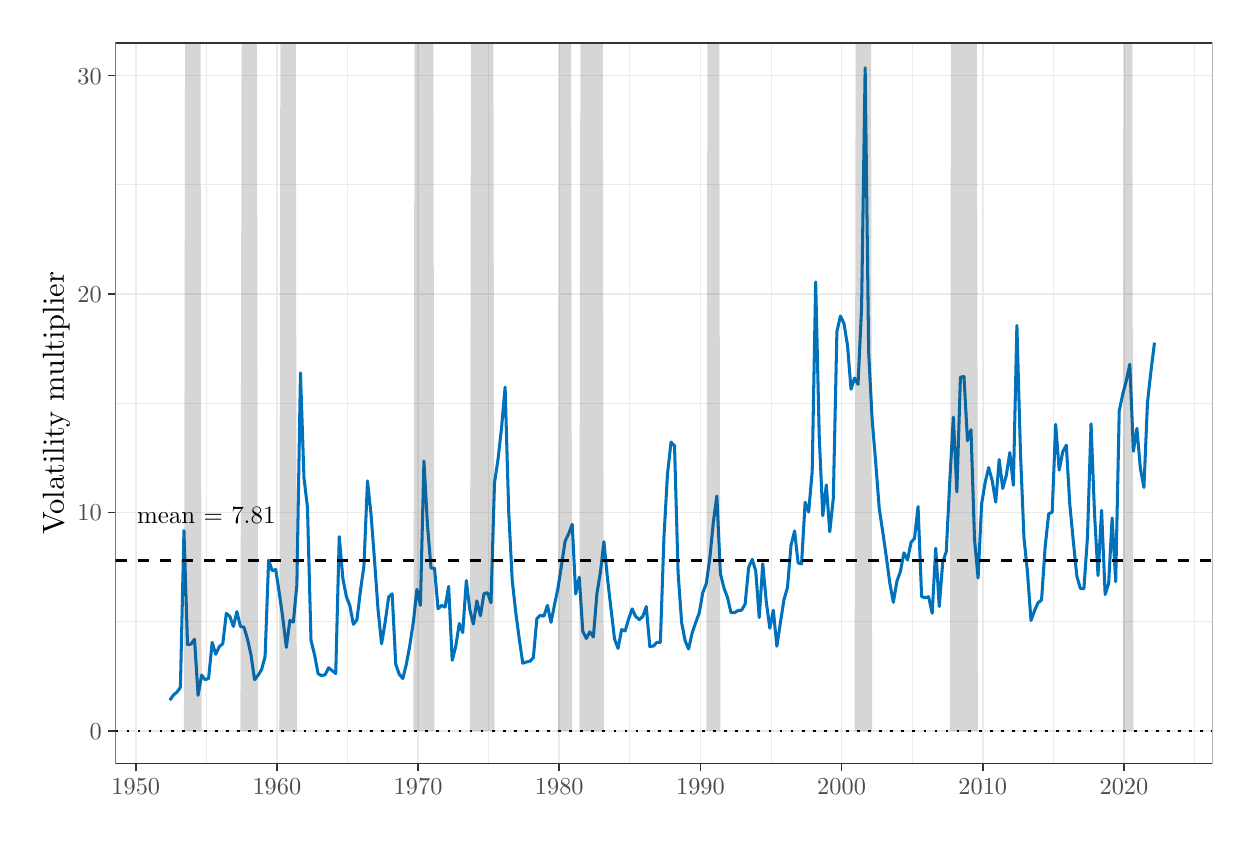
\begin{tikzpicture}[x=1pt,y=1pt]
\definecolor{fillColor}{RGB}{255,255,255}
\path[use as bounding box,fill=fillColor,fill opacity=0.00] (0,0) rectangle (433.62,289.08);
\begin{scope}
\path[clip] (  0.00,  0.00) rectangle (433.62,289.08);
\definecolor{drawColor}{RGB}{255,255,255}
\definecolor{fillColor}{RGB}{255,255,255}

\path[draw=drawColor,line width= 0.6pt,line join=round,line cap=round,fill=fillColor] (  0.00,  0.00) rectangle (433.62,289.08);
\end{scope}
\begin{scope}
\path[clip] ( 31.71, 23.11) rectangle (428.12,283.58);
\definecolor{fillColor}{RGB}{255,255,255}

\path[fill=fillColor] ( 31.71, 23.11) rectangle (428.12,283.58);
\definecolor{drawColor}{gray}{0.92}

\path[draw=drawColor,line width= 0.3pt,line join=round] ( 31.71, 74.41) --
	(428.12, 74.41);

\path[draw=drawColor,line width= 0.3pt,line join=round] ( 31.71,153.34) --
	(428.12,153.34);

\path[draw=drawColor,line width= 0.3pt,line join=round] ( 31.71,232.28) --
	(428.12,232.28);

\path[draw=drawColor,line width= 0.3pt,line join=round] ( 64.56, 23.11) --
	( 64.56,283.58);

\path[draw=drawColor,line width= 0.3pt,line join=round] (115.57, 23.11) --
	(115.57,283.58);

\path[draw=drawColor,line width= 0.3pt,line join=round] (166.59, 23.11) --
	(166.59,283.58);

\path[draw=drawColor,line width= 0.3pt,line join=round] (217.60, 23.11) --
	(217.60,283.58);

\path[draw=drawColor,line width= 0.3pt,line join=round] (268.61, 23.11) --
	(268.61,283.58);

\path[draw=drawColor,line width= 0.3pt,line join=round] (319.62, 23.11) --
	(319.62,283.58);

\path[draw=drawColor,line width= 0.3pt,line join=round] (370.64, 23.11) --
	(370.64,283.58);

\path[draw=drawColor,line width= 0.3pt,line join=round] (421.64, 23.11) --
	(421.64,283.58);

\path[draw=drawColor,line width= 0.6pt,line join=round] ( 31.71, 34.95) --
	(428.12, 34.95);

\path[draw=drawColor,line width= 0.6pt,line join=round] ( 31.71,113.88) --
	(428.12,113.88);

\path[draw=drawColor,line width= 0.6pt,line join=round] ( 31.71,192.81) --
	(428.12,192.81);

\path[draw=drawColor,line width= 0.6pt,line join=round] ( 31.71,271.74) --
	(428.12,271.74);

\path[draw=drawColor,line width= 0.6pt,line join=round] ( 39.06, 23.11) --
	( 39.06,283.58);

\path[draw=drawColor,line width= 0.6pt,line join=round] ( 90.06, 23.11) --
	( 90.06,283.58);

\path[draw=drawColor,line width= 0.6pt,line join=round] (141.08, 23.11) --
	(141.08,283.58);

\path[draw=drawColor,line width= 0.6pt,line join=round] (192.09, 23.11) --
	(192.09,283.58);

\path[draw=drawColor,line width= 0.6pt,line join=round] (243.11, 23.11) --
	(243.11,283.58);

\path[draw=drawColor,line width= 0.6pt,line join=round] (294.11, 23.11) --
	(294.11,283.58);

\path[draw=drawColor,line width= 0.6pt,line join=round] (345.13, 23.11) --
	(345.13,283.58);

\path[draw=drawColor,line width= 0.6pt,line join=round] (396.14, 23.11) --
	(396.14,283.58);
\definecolor{drawColor}{RGB}{0,114,189}

\path[draw=drawColor,line width= 1.1pt,line join=round] ( 51.38, 46.04) --
	( 52.66, 47.92) --
	( 53.93, 48.94) --
	( 55.19, 50.73) --
	( 56.47,107.36) --
	( 57.76, 66.17) --
	( 59.03, 66.34) --
	( 60.29, 68.09) --
	( 61.57, 47.82) --
	( 62.86, 55.13) --
	( 64.13, 53.47) --
	( 65.38, 53.96) --
	( 66.67, 66.96) --
	( 67.95, 62.65) --
	( 69.22, 65.38) --
	( 70.50, 66.45) --
	( 71.78, 77.44) --
	( 73.07, 76.31) --
	( 74.34, 72.68) --
	( 75.59, 78.09) --
	( 76.88, 72.69) --
	( 78.16, 72.45) --
	( 79.43, 68.14) --
	( 80.69, 62.51) --
	( 81.98, 53.49) --
	( 83.26, 55.04) --
	( 84.53, 57.15) --
	( 85.79, 61.88) --
	( 87.07, 96.65) --
	( 88.36, 92.86) --
	( 89.63, 93.25) --
	( 90.90, 84.90) --
	( 92.19, 75.80) --
	( 93.47, 65.15) --
	( 94.74, 74.90) --
	( 96.00, 74.28) --
	( 97.28, 87.82) --
	( 98.57,164.32) --
	( 99.84,126.39) --
	(101.10,115.80) --
	(102.38, 67.66) --
	(103.67, 62.44) --
	(104.94, 55.65) --
	(106.19, 54.93) --
	(107.48, 55.25) --
	(108.76, 57.79) --
	(110.03, 56.74) --
	(111.31, 55.69) --
	(112.59,105.19) --
	(113.88, 90.17) --
	(115.15, 83.51) --
	(116.40, 80.30) --
	(117.69, 73.48) --
	(118.97, 75.10) --
	(120.24, 85.61) --
	(121.50, 94.53) --
	(122.79,125.28) --
	(124.07,113.29) --
	(125.34, 96.52) --
	(126.60, 78.82) --
	(127.88, 66.42) --
	(129.17, 74.21) --
	(130.44, 83.33) --
	(131.71, 84.53) --
	(133.00, 59.04) --
	(134.28, 55.40) --
	(135.55, 53.88) --
	(136.81, 59.00) --
	(138.09, 65.88) --
	(139.38, 74.47) --
	(140.65, 86.13) --
	(141.91, 80.35) --
	(143.19,132.47) --
	(144.48,109.11) --
	(145.75, 93.79) --
	(147.00, 93.81) --
	(148.29, 79.11) --
	(149.57, 80.33) --
	(150.84, 79.69) --
	(152.12, 87.19) --
	(153.40, 60.48) --
	(154.69, 65.54) --
	(155.96, 73.79) --
	(157.21, 70.50) --
	(158.50, 89.30) --
	(159.78, 78.62) --
	(161.05, 73.57) --
	(162.31, 81.95) --
	(163.60, 76.57) --
	(164.88, 84.54) --
	(166.15, 84.92) --
	(167.41, 81.25) --
	(168.69,124.67) --
	(169.98,133.24) --
	(171.25,144.72) --
	(172.52,159.20) --
	(173.81,114.41) --
	(175.09, 89.36) --
	(176.36, 77.86) --
	(177.62, 68.31) --
	(178.90, 59.44) --
	(180.19, 59.86) --
	(181.46, 60.11) --
	(182.72, 61.41) --
	(184.00, 75.59) --
	(185.29, 76.77) --
	(186.56, 76.43) --
	(187.81, 80.34) --
	(189.10, 74.19) --
	(190.38, 80.62) --
	(191.65, 86.70) --
	(192.93, 95.02) --
	(194.21,103.55) --
	(195.50,106.24) --
	(196.77,109.62) --
	(198.02, 84.44) --
	(199.31, 90.53) --
	(200.59, 70.97) --
	(201.86, 68.37) --
	(203.12, 70.77) --
	(204.41, 68.90) --
	(205.69, 84.51) --
	(206.96, 92.28) --
	(208.22,103.34) --
	(209.50, 90.26) --
	(210.79, 79.02) --
	(212.06, 68.19) --
	(213.33, 64.78) --
	(214.62, 71.59) --
	(215.90, 71.11) --
	(217.17, 75.45) --
	(218.43, 79.06) --
	(219.71, 76.33) --
	(221.00, 75.14) --
	(222.27, 76.35) --
	(223.53, 79.89) --
	(224.81, 65.43) --
	(226.10, 65.65) --
	(227.37, 66.94) --
	(228.62, 66.92) --
	(229.91,104.88) --
	(231.19,127.79) --
	(232.47,139.32) --
	(233.74,137.96) --
	(235.02, 92.13) --
	(236.31, 74.07) --
	(237.58, 67.51) --
	(238.83, 64.58) --
	(240.12, 70.42) --
	(241.40, 74.14) --
	(242.67, 77.61) --
	(243.93, 84.85) --
	(245.22, 88.23) --
	(246.50, 97.43) --
	(247.77,110.46) --
	(249.03,119.86) --
	(250.31, 91.89) --
	(251.60, 86.58) --
	(252.87, 83.20) --
	(254.14, 77.70) --
	(255.43, 77.71) --
	(256.71, 78.46) --
	(257.98, 78.60) --
	(259.24, 80.78) --
	(260.52, 94.01) --
	(261.81, 96.94) --
	(263.08, 92.79) --
	(264.34, 75.94) --
	(265.62, 95.34) --
	(266.91, 81.41) --
	(268.18, 72.06) --
	(269.43, 78.57) --
	(270.72, 65.55) --
	(272.00, 74.10) --
	(273.28, 82.34) --
	(274.55, 86.82) --
	(275.83,102.05) --
	(277.12,107.22) --
	(278.39, 95.68) --
	(279.64, 95.33) --
	(280.93,117.59) --
	(282.21,114.06) --
	(283.48,128.77) --
	(284.74,197.19) --
	(286.03,141.29) --
	(287.31,112.71) --
	(288.58,123.87) --
	(289.84,106.92) --
	(291.12,119.08) --
	(292.41,179.23) --
	(293.68,184.88) --
	(294.95,182.22) --
	(296.24,174.31) --
	(297.52,158.42) --
	(298.79,162.48) --
	(300.05,160.19) --
	(301.33,187.92) --
	(302.62,274.60) --
	(303.89,171.71) --
	(305.15,147.57) --
	(306.43,131.95) --
	(307.72,115.27) --
	(308.99,106.81) --
	(310.24, 98.00) --
	(311.53, 88.40) --
	(312.81, 81.43) --
	(314.09, 89.07) --
	(315.36, 92.56) --
	(316.64, 99.33) --
	(317.93, 96.72) --
	(319.20,103.10) --
	(320.45,104.53) --
	(321.74,116.02) --
	(323.02, 83.51) --
	(324.29, 83.06) --
	(325.55, 83.43) --
	(326.84, 77.46) --
	(328.12,100.99) --
	(329.39, 79.90) --
	(330.65, 95.92) --
	(331.93, 99.75) --
	(333.22,125.71) --
	(334.49,148.38) --
	(335.76,121.34) --
	(337.05,162.78) --
	(338.33,163.01) --
	(339.60,139.83) --
	(340.86,143.81) --
	(342.14,104.14) --
	(343.43, 90.21) --
	(344.70,116.95) --
	(345.96,124.65) --
	(347.24,130.15) --
	(348.53,125.38) --
	(349.80,117.64) --
	(351.05,133.01) --
	(352.34,122.57) --
	(353.62,127.25) --
	(354.90,135.57) --
	(356.17,123.71) --
	(357.45,181.47) --
	(358.74,135.49) --
	(360.01,104.75) --
	(361.26, 92.42) --
	(362.55, 74.86) --
	(363.83, 78.44) --
	(365.10, 81.29) --
	(366.36, 82.26) --
	(367.65,101.35) --
	(368.93,113.41) --
	(370.20,113.98) --
	(371.46,145.74) --
	(372.74,129.18) --
	(374.03,135.87) --
	(375.30,138.21) --
	(376.57,116.84) --
	(377.86,103.29) --
	(379.14, 90.72) --
	(380.41, 86.41) --
	(381.67, 86.35) --
	(382.95,104.94) --
	(384.24,145.94) --
	(385.51,113.26) --
	(386.77, 91.11) --
	(388.05,114.68) --
	(389.34, 84.25) --
	(390.61, 88.31) --
	(391.86,111.92) --
	(393.15, 88.88) --
	(394.43,150.61) --
	(395.71,156.70) --
	(396.98,161.47) --
	(398.26,167.46) --
	(399.55,136.03) --
	(400.82,144.31) --
	(402.07,129.83) --
	(403.36,122.94) --
	(404.64,153.67) --
	(405.91,165.12) --
	(407.17,175.26);
\definecolor{fillColor}{RGB}{51,51,51}

\path[fill=fillColor,fill opacity=0.20] ( 50.09, 34.95) --
	( 50.45, 34.95) --
	( 51.02, 34.95) --
	( 51.38, 34.95) --
	( 51.73, 34.95) --
	( 52.30, 34.95) --
	( 52.66, 34.95) --
	( 53.02, 34.95) --
	( 53.57, 34.95) --
	( 53.93, 34.95) --
	( 54.29, 34.95) --
	( 54.83, 34.95) --
	( 55.19, 34.95) --
	( 55.55, 34.95) --
	( 56.11, 34.95) --
	( 56.47, 34.95) --
	( 56.83,255.88) --
	( 57.40,603.33) --
	( 57.76,824.25) --
	( 58.12,824.25) --
	( 58.67,824.25) --
	( 59.03,824.25) --
	( 59.39,824.25) --
	( 59.93,824.25) --
	( 60.29,824.25) --
	( 60.65,824.25) --
	( 61.21,824.25) --
	( 61.57,824.25) --
	( 61.93,603.33) --
	( 62.50,255.88) --
	( 62.86, 34.95) --
	( 63.22, 34.95) --
	( 63.77, 34.95) --
	( 64.13, 34.95) --
	( 64.49, 34.95) --
	( 65.02, 34.95) --
	( 65.38, 34.95) --
	( 65.74, 34.95) --
	( 66.31, 34.95) --
	( 66.67, 34.95) --
	( 67.03, 34.95) --
	( 67.59, 34.95) --
	( 67.95, 34.95) --
	( 68.31, 34.95) --
	( 68.86, 34.95) --
	( 69.22, 34.95) --
	( 69.58, 34.95) --
	( 70.14, 34.95) --
	( 70.50, 34.95) --
	( 70.86, 34.95) --
	( 71.42, 34.95) --
	( 71.78, 34.95) --
	( 72.14, 34.95) --
	( 72.71, 34.95) --
	( 73.07, 34.95) --
	( 73.42, 34.95) --
	( 73.98, 34.95) --
	( 74.34, 34.95) --
	( 74.70, 34.95) --
	( 75.23, 34.95) --
	( 75.59, 34.95) --
	( 75.95, 34.95) --
	( 76.52, 34.95) --
	( 76.88, 34.95) --
	( 77.24,255.88) --
	( 77.80,603.33) --
	( 78.16,824.25) --
	( 78.52,824.25) --
	( 79.07,824.25) --
	( 79.43,824.25) --
	( 79.79,824.25) --
	( 80.33,824.25) --
	( 80.69,824.25) --
	( 81.05,824.25) --
	( 81.62,824.25) --
	( 81.98,824.25) --
	( 82.34,603.33) --
	( 82.90,255.88) --
	( 83.26, 34.95) --
	( 83.62, 34.95) --
	( 84.17, 34.95) --
	( 84.53, 34.95) --
	( 84.89, 34.95) --
	( 85.43, 34.95) --
	( 85.79, 34.95) --
	( 86.15, 34.95) --
	( 86.71, 34.95) --
	( 87.07, 34.95) --
	( 87.43, 34.95) --
	( 88.00, 34.95) --
	( 88.36, 34.95) --
	( 88.72, 34.95) --
	( 89.27, 34.95) --
	( 89.63, 34.95) --
	( 89.99, 34.95) --
	( 90.54, 34.95) --
	( 90.90, 34.95) --
	( 91.26,255.88) --
	( 91.83,603.33) --
	( 92.19,824.25) --
	( 92.55,824.25) --
	( 93.11,824.25) --
	( 93.47,824.25) --
	( 93.83,824.25) --
	( 94.38,824.25) --
	( 94.74,824.25) --
	( 95.10,824.25) --
	( 95.64,824.25) --
	( 96.00,824.25) --
	( 96.36,603.33) --
	( 96.92,255.88) --
	( 97.28, 34.95) --
	( 97.64, 34.95) --
	( 98.21, 34.95) --
	( 98.57, 34.95) --
	( 98.93, 34.95) --
	( 99.48, 34.95) --
	( 99.84, 34.95) --
	(100.20, 34.95) --
	(100.74, 34.95) --
	(101.10, 34.95) --
	(101.46, 34.95) --
	(102.02, 34.95) --
	(102.38, 34.95) --
	(102.74, 34.95) --
	(103.31, 34.95) --
	(103.67, 34.95) --
	(104.03, 34.95) --
	(104.58, 34.95) --
	(104.94, 34.95) --
	(105.30, 34.95) --
	(105.83, 34.95) --
	(106.19, 34.95) --
	(106.55, 34.95) --
	(107.12, 34.95) --
	(107.48, 34.95) --
	(107.84, 34.95) --
	(108.40, 34.95) --
	(108.76, 34.95) --
	(109.12, 34.95) --
	(109.67, 34.95) --
	(110.03, 34.95) --
	(110.39, 34.95) --
	(110.95, 34.95) --
	(111.31, 34.95) --
	(111.67, 34.95) --
	(112.23, 34.95) --
	(112.59, 34.95) --
	(112.95, 34.95) --
	(113.52, 34.95) --
	(113.88, 34.95) --
	(114.24, 34.95) --
	(114.79, 34.95) --
	(115.15, 34.95) --
	(115.51, 34.95) --
	(116.04, 34.95) --
	(116.40, 34.95) --
	(116.76, 34.95) --
	(117.33, 34.95) --
	(117.69, 34.95) --
	(118.05, 34.95) --
	(118.61, 34.95) --
	(118.97, 34.95) --
	(119.33, 34.95) --
	(119.88, 34.95) --
	(120.24, 34.95) --
	(120.60, 34.95) --
	(121.14, 34.95) --
	(121.50, 34.95) --
	(121.86, 34.95) --
	(122.43, 34.95) --
	(122.79, 34.95) --
	(123.15, 34.95) --
	(123.71, 34.95) --
	(124.07, 34.95) --
	(124.43, 34.95) --
	(124.98, 34.95) --
	(125.34, 34.95) --
	(125.70, 34.95) --
	(126.24, 34.95) --
	(126.60, 34.95) --
	(126.96, 34.95) --
	(127.52, 34.95) --
	(127.88, 34.95) --
	(128.24, 34.95) --
	(128.81, 34.95) --
	(129.17, 34.95) --
	(129.53, 34.95) --
	(130.08, 34.95) --
	(130.44, 34.95) --
	(130.80, 34.95) --
	(131.35, 34.95) --
	(131.71, 34.95) --
	(132.07, 34.95) --
	(132.64, 34.95) --
	(133.00, 34.95) --
	(133.36, 34.95) --
	(133.92, 34.95) --
	(134.28, 34.95) --
	(134.64, 34.95) --
	(135.19, 34.95) --
	(135.55, 34.95) --
	(135.91, 34.95) --
	(136.45, 34.95) --
	(136.81, 34.95) --
	(137.17, 34.95) --
	(137.73, 34.95) --
	(138.09, 34.95) --
	(138.45, 34.95) --
	(139.02, 34.95) --
	(139.38, 34.95) --
	(139.74,258.30) --
	(140.29,600.90) --
	(140.65,824.25) --
	(141.01,824.25) --
	(141.55,824.25) --
	(141.91,824.25) --
	(142.27,824.25) --
	(142.83,824.25) --
	(143.19,824.25) --
	(143.55,824.25) --
	(144.12,824.25) --
	(144.48,824.25) --
	(144.84,824.25) --
	(145.39,824.25) --
	(145.75,824.25) --
	(146.11,598.42) --
	(146.64,260.79) --
	(147.00, 34.95) --
	(147.36, 34.95) --
	(147.93, 34.95) --
	(148.29, 34.95) --
	(148.65, 34.95) --
	(149.21, 34.95) --
	(149.57, 34.95) --
	(149.93, 34.95) --
	(150.49, 34.95) --
	(150.84, 34.95) --
	(151.20, 34.95) --
	(151.76, 34.95) --
	(152.12, 34.95) --
	(152.48, 34.95) --
	(153.04, 34.95) --
	(153.40, 34.95) --
	(153.76, 34.95) --
	(154.33, 34.95) --
	(154.69, 34.95) --
	(155.05, 34.95) --
	(155.60, 34.95) --
	(155.96, 34.95) --
	(156.32, 34.95) --
	(156.85, 34.95) --
	(157.21, 34.95) --
	(157.57, 34.95) --
	(158.14, 34.95) --
	(158.50, 34.95) --
	(158.86, 34.95) --
	(159.42, 34.95) --
	(159.78, 34.95) --
	(160.14,258.30) --
	(160.69,600.90) --
	(161.05,824.25) --
	(161.41,824.25) --
	(161.95,824.25) --
	(162.31,824.25) --
	(162.67,824.25) --
	(163.24,824.25) --
	(163.60,824.25) --
	(163.96,824.25) --
	(164.52,824.25) --
	(164.88,824.25) --
	(165.24,824.25) --
	(165.79,824.25) --
	(166.15,824.25) --
	(166.51,824.25) --
	(167.05,824.25) --
	(167.41,824.25) --
	(167.77,603.33) --
	(168.33,255.88) --
	(168.69, 34.95) --
	(169.05, 34.95) --
	(169.62, 34.95) --
	(169.98, 34.95) --
	(170.34, 34.95) --
	(170.89, 34.95) --
	(171.25, 34.95) --
	(171.61, 34.95) --
	(172.16, 34.95) --
	(172.52, 34.95) --
	(172.88, 34.95) --
	(173.45, 34.95) --
	(173.81, 34.95) --
	(174.17, 34.95) --
	(174.73, 34.95) --
	(175.09, 34.95) --
	(175.45, 34.95) --
	(176.00, 34.95) --
	(176.36, 34.95) --
	(176.72, 34.95) --
	(177.26, 34.95) --
	(177.62, 34.95) --
	(177.98, 34.95) --
	(178.54, 34.95) --
	(178.90, 34.95) --
	(179.26, 34.95) --
	(179.83, 34.95) --
	(180.19, 34.95) --
	(180.55, 34.95) --
	(181.10, 34.95) --
	(181.46, 34.95) --
	(181.82, 34.95) --
	(182.36, 34.95) --
	(182.72, 34.95) --
	(183.08, 34.95) --
	(183.64, 34.95) --
	(184.00, 34.95) --
	(184.36, 34.95) --
	(184.93, 34.95) --
	(185.29, 34.95) --
	(185.65, 34.95) --
	(186.20, 34.95) --
	(186.56, 34.95) --
	(186.92, 34.95) --
	(187.45, 34.95) --
	(187.81, 34.95) --
	(188.17, 34.95) --
	(188.74, 34.95) --
	(189.10, 34.95) --
	(189.46, 34.95) --
	(190.02, 34.95) --
	(190.38, 34.95) --
	(190.74, 34.95) --
	(191.30, 34.95) --
	(191.65, 34.95) --
	(192.01,258.30) --
	(192.57,600.90) --
	(192.93,824.25) --
	(193.29,824.25) --
	(193.85,824.25) --
	(194.21,824.25) --
	(194.57,824.25) --
	(195.14,824.25) --
	(195.50,824.25) --
	(195.86,600.90) --
	(196.41,258.30) --
	(196.77, 34.95) --
	(197.13, 34.95) --
	(197.66, 34.95) --
	(198.02, 34.95) --
	(198.38, 34.95) --
	(198.95, 34.95) --
	(199.31, 34.95) --
	(199.67,255.88) --
	(200.23,603.33) --
	(200.59,824.25) --
	(200.95,824.25) --
	(201.50,824.25) --
	(201.86,824.25) --
	(202.22,824.25) --
	(202.76,824.25) --
	(203.12,824.25) --
	(203.48,824.25) --
	(204.05,824.25) --
	(204.41,824.25) --
	(204.77,824.25) --
	(205.33,824.25) --
	(205.69,824.25) --
	(206.05,824.25) --
	(206.60,824.25) --
	(206.96,824.25) --
	(207.32,598.42) --
	(207.86,260.79) --
	(208.22, 34.95) --
	(208.58, 34.95) --
	(209.14, 34.95) --
	(209.50, 34.95) --
	(209.86, 34.95) --
	(210.43, 34.95) --
	(210.79, 34.95) --
	(211.15, 34.95) --
	(211.70, 34.95) --
	(212.06, 34.95) --
	(212.42, 34.95) --
	(212.97, 34.95) --
	(213.33, 34.95) --
	(213.69, 34.95) --
	(214.26, 34.95) --
	(214.62, 34.95) --
	(214.98, 34.95) --
	(215.54, 34.95) --
	(215.90, 34.95) --
	(216.26, 34.95) --
	(216.81, 34.95) --
	(217.17, 34.95) --
	(217.53, 34.95) --
	(218.07, 34.95) --
	(218.43, 34.95) --
	(218.79, 34.95) --
	(219.35, 34.95) --
	(219.71, 34.95) --
	(220.07, 34.95) --
	(220.64, 34.95) --
	(221.00, 34.95) --
	(221.36, 34.95) --
	(221.91, 34.95) --
	(222.27, 34.95) --
	(222.63, 34.95) --
	(223.17, 34.95) --
	(223.53, 34.95) --
	(223.89, 34.95) --
	(224.45, 34.95) --
	(224.81, 34.95) --
	(225.17, 34.95) --
	(225.74, 34.95) --
	(226.10, 34.95) --
	(226.46, 34.95) --
	(227.01, 34.95) --
	(227.37, 34.95) --
	(227.73, 34.95) --
	(228.26, 34.95) --
	(228.62, 34.95) --
	(228.98, 34.95) --
	(229.55, 34.95) --
	(229.91, 34.95) --
	(230.27, 34.95) --
	(230.83, 34.95) --
	(231.19, 34.95) --
	(231.55, 34.95) --
	(232.11, 34.95) --
	(232.47, 34.95) --
	(232.82, 34.95) --
	(233.38, 34.95) --
	(233.74, 34.95) --
	(234.10, 34.95) --
	(234.66, 34.95) --
	(235.02, 34.95) --
	(235.38, 34.95) --
	(235.95, 34.95) --
	(236.31, 34.95) --
	(236.67, 34.95) --
	(237.22, 34.95) --
	(237.58, 34.95) --
	(237.94, 34.95) --
	(238.47, 34.95) --
	(238.83, 34.95) --
	(239.19, 34.95) --
	(239.76, 34.95) --
	(240.12, 34.95) --
	(240.48, 34.95) --
	(241.04, 34.95) --
	(241.40, 34.95) --
	(241.76, 34.95) --
	(242.31, 34.95) --
	(242.67, 34.95) --
	(243.03, 34.95) --
	(243.57, 34.95) --
	(243.93, 34.95) --
	(244.29, 34.95) --
	(244.86, 34.95) --
	(245.22, 34.95) --
	(245.58,255.88) --
	(246.14,603.33) --
	(246.50,824.25) --
	(246.86,824.25) --
	(247.41,824.25) --
	(247.77,824.25) --
	(248.13,824.25) --
	(248.67,824.25) --
	(249.03,824.25) --
	(249.39,603.33) --
	(249.95,255.88) --
	(250.31, 34.95) --
	(250.67, 34.95) --
	(251.24, 34.95) --
	(251.60, 34.95) --
	(251.96, 34.95) --
	(252.51, 34.95) --
	(252.87, 34.95) --
	(253.23, 34.95) --
	(253.78, 34.95) --
	(254.14, 34.95) --
	(254.50, 34.95) --
	(255.07, 34.95) --
	(255.43, 34.95) --
	(255.79, 34.95) --
	(256.35, 34.95) --
	(256.71, 34.95) --
	(257.07, 34.95) --
	(257.62, 34.95) --
	(257.98, 34.95) --
	(258.34, 34.95) --
	(258.88, 34.95) --
	(259.24, 34.95) --
	(259.60, 34.95) --
	(260.16, 34.95) --
	(260.52, 34.95) --
	(260.88, 34.95) --
	(261.45, 34.95) --
	(261.81, 34.95) --
	(262.17, 34.95) --
	(262.72, 34.95) --
	(263.08, 34.95) --
	(263.44, 34.95) --
	(263.98, 34.95) --
	(264.34, 34.95) --
	(264.70, 34.95) --
	(265.26, 34.95) --
	(265.62, 34.95) --
	(265.98, 34.95) --
	(266.55, 34.95) --
	(266.91, 34.95) --
	(267.27, 34.95) --
	(267.82, 34.95) --
	(268.18, 34.95) --
	(268.54, 34.95) --
	(269.07, 34.95) --
	(269.43, 34.95) --
	(269.79, 34.95) --
	(270.36, 34.95) --
	(270.72, 34.95) --
	(271.08, 34.95) --
	(271.64, 34.95) --
	(272.00, 34.95) --
	(272.36, 34.95) --
	(272.92, 34.95) --
	(273.28, 34.95) --
	(273.63, 34.95) --
	(274.19, 34.95) --
	(274.55, 34.95) --
	(274.91, 34.95) --
	(275.47, 34.95) --
	(275.83, 34.95) --
	(276.19, 34.95) --
	(276.76, 34.95) --
	(277.12, 34.95) --
	(277.48, 34.95) --
	(278.03, 34.95) --
	(278.39, 34.95) --
	(278.75, 34.95) --
	(279.28, 34.95) --
	(279.64, 34.95) --
	(280.00, 34.95) --
	(280.57, 34.95) --
	(280.93, 34.95) --
	(281.29, 34.95) --
	(281.85, 34.95) --
	(282.21, 34.95) --
	(282.57, 34.95) --
	(283.12, 34.95) --
	(283.48, 34.95) --
	(283.84, 34.95) --
	(284.38, 34.95) --
	(284.74, 34.95) --
	(285.10, 34.95) --
	(285.67, 34.95) --
	(286.03, 34.95) --
	(286.39, 34.95) --
	(286.95, 34.95) --
	(287.31, 34.95) --
	(287.67, 34.95) --
	(288.22, 34.95) --
	(288.58, 34.95) --
	(288.94, 34.95) --
	(289.48, 34.95) --
	(289.84, 34.95) --
	(290.20, 34.95) --
	(290.76, 34.95) --
	(291.12, 34.95) --
	(291.48, 34.95) --
	(292.05, 34.95) --
	(292.41, 34.95) --
	(292.77, 34.95) --
	(293.32, 34.95) --
	(293.68, 34.95) --
	(294.04, 34.95) --
	(294.59, 34.95) --
	(294.95, 34.95) --
	(295.31, 34.95) --
	(295.88, 34.95) --
	(296.24, 34.95) --
	(296.60, 34.95) --
	(297.16, 34.95) --
	(297.52, 34.95) --
	(297.88, 34.95) --
	(298.43, 34.95) --
	(298.79, 34.95) --
	(299.15,260.79) --
	(299.69,598.42) --
	(300.05,824.25) --
	(300.41,824.25) --
	(300.97,824.25) --
	(301.33,824.25) --
	(301.69,824.25) --
	(302.26,824.25) --
	(302.62,824.25) --
	(302.98,824.25) --
	(303.53,824.25) --
	(303.89,824.25) --
	(304.25,598.42) --
	(304.79,260.79) --
	(305.15, 34.95) --
	(305.51, 34.95) --
	(306.07, 34.95) --
	(306.43, 34.95) --
	(306.79, 34.95) --
	(307.36, 34.95) --
	(307.72, 34.95) --
	(308.08, 34.95) --
	(308.63, 34.95) --
	(308.99, 34.95) --
	(309.35, 34.95) --
	(309.88, 34.95) --
	(310.24, 34.95) --
	(310.60, 34.95) --
	(311.17, 34.95) --
	(311.53, 34.95) --
	(311.89, 34.95) --
	(312.45, 34.95) --
	(312.81, 34.95) --
	(313.17, 34.95) --
	(313.73, 34.95) --
	(314.09, 34.95) --
	(314.44, 34.95) --
	(315.00, 34.95) --
	(315.36, 34.95) --
	(315.72, 34.95) --
	(316.28, 34.95) --
	(316.64, 34.95) --
	(317.00, 34.95) --
	(317.57, 34.95) --
	(317.93, 34.95) --
	(318.29, 34.95) --
	(318.84, 34.95) --
	(319.20, 34.95) --
	(319.56, 34.95) --
	(320.09, 34.95) --
	(320.45, 34.95) --
	(320.81, 34.95) --
	(321.38, 34.95) --
	(321.74, 34.95) --
	(322.10, 34.95) --
	(322.66, 34.95) --
	(323.02, 34.95) --
	(323.38, 34.95) --
	(323.94, 34.95) --
	(324.29, 34.95) --
	(324.65, 34.95) --
	(325.19, 34.95) --
	(325.55, 34.95) --
	(325.91, 34.95) --
	(326.48, 34.95) --
	(326.84, 34.95) --
	(327.20, 34.95) --
	(327.76, 34.95) --
	(328.12, 34.95) --
	(328.48, 34.95) --
	(329.03, 34.95) --
	(329.39, 34.95) --
	(329.75, 34.95) --
	(330.29, 34.95) --
	(330.65, 34.95) --
	(331.01, 34.95) --
	(331.57, 34.95) --
	(331.93, 34.95) --
	(332.29, 34.95) --
	(332.86, 34.95) --
	(333.22, 34.95) --
	(333.58,258.30) --
	(334.13,600.90) --
	(334.49,824.25) --
	(334.85,824.25) --
	(335.40,824.25) --
	(335.76,824.25) --
	(336.12,824.25) --
	(336.69,824.25) --
	(337.05,824.25) --
	(337.41,824.25) --
	(337.97,824.25) --
	(338.33,824.25) --
	(338.69,824.25) --
	(339.24,824.25) --
	(339.60,824.25) --
	(339.96,824.25) --
	(340.50,824.25) --
	(340.86,824.25) --
	(341.22,824.25) --
	(341.78,824.25) --
	(342.14,824.25) --
	(342.50,603.33) --
	(343.07,255.88) --
	(343.43, 34.95) --
	(343.79, 34.95) --
	(344.34, 34.95) --
	(344.70, 34.95) --
	(345.06, 34.95) --
	(345.60, 34.95) --
	(345.96, 34.95) --
	(346.32, 34.95) --
	(346.88, 34.95) --
	(347.24, 34.95) --
	(347.60, 34.95) --
	(348.17, 34.95) --
	(348.53, 34.95) --
	(348.89, 34.95) --
	(349.44, 34.95) --
	(349.80, 34.95) --
	(350.16, 34.95) --
	(350.69, 34.95) --
	(351.05, 34.95) --
	(351.41, 34.95) --
	(351.98, 34.95) --
	(352.34, 34.95) --
	(352.70, 34.95) --
	(353.26, 34.95) --
	(353.62, 34.95) --
	(353.98, 34.95) --
	(354.54, 34.95) --
	(354.90, 34.95) --
	(355.26, 34.95) --
	(355.81, 34.95) --
	(356.17, 34.95) --
	(356.53, 34.95) --
	(357.09, 34.95) --
	(357.45, 34.95) --
	(357.81, 34.95) --
	(358.38, 34.95) --
	(358.74, 34.95) --
	(359.10, 34.95) --
	(359.65, 34.95) --
	(360.01, 34.95) --
	(360.37, 34.95) --
	(360.90, 34.95) --
	(361.26, 34.95) --
	(361.62, 34.95) --
	(362.19, 34.95) --
	(362.55, 34.95) --
	(362.91, 34.95) --
	(363.47, 34.95) --
	(363.83, 34.95) --
	(364.19, 34.95) --
	(364.75, 34.95) --
	(365.10, 34.95) --
	(365.46, 34.95) --
	(366.00, 34.95) --
	(366.36, 34.95) --
	(366.72, 34.95) --
	(367.29, 34.95) --
	(367.65, 34.95) --
	(368.01, 34.95) --
	(368.57, 34.95) --
	(368.93, 34.95) --
	(369.29, 34.95) --
	(369.84, 34.95) --
	(370.20, 34.95) --
	(370.56, 34.95) --
	(371.10, 34.95) --
	(371.46, 34.95) --
	(371.82, 34.95) --
	(372.38, 34.95) --
	(372.74, 34.95) --
	(373.10, 34.95) --
	(373.67, 34.95) --
	(374.03, 34.95) --
	(374.39, 34.95) --
	(374.94, 34.95) --
	(375.30, 34.95) --
	(375.66, 34.95) --
	(376.21, 34.95) --
	(376.57, 34.95) --
	(376.93, 34.95) --
	(377.50, 34.95) --
	(377.86, 34.95) --
	(378.22, 34.95) --
	(378.78, 34.95) --
	(379.14, 34.95) --
	(379.50, 34.95) --
	(380.05, 34.95) --
	(380.41, 34.95) --
	(380.77, 34.95) --
	(381.31, 34.95) --
	(381.67, 34.95) --
	(382.03, 34.95) --
	(382.59, 34.95) --
	(382.95, 34.95) --
	(383.31, 34.95) --
	(383.88, 34.95) --
	(384.24, 34.95) --
	(384.60, 34.95) --
	(385.15, 34.95) --
	(385.51, 34.95) --
	(385.87, 34.95) --
	(386.41, 34.95) --
	(386.77, 34.95) --
	(387.13, 34.95) --
	(387.69, 34.95) --
	(388.05, 34.95) --
	(388.41, 34.95) --
	(388.98, 34.95) --
	(389.34, 34.95) --
	(389.70, 34.95) --
	(390.25, 34.95) --
	(390.61, 34.95) --
	(390.97, 34.95) --
	(391.51, 34.95) --
	(391.86, 34.95) --
	(392.22, 34.95) --
	(392.79, 34.95) --
	(393.15, 34.95) --
	(393.51, 34.95) --
	(394.07, 34.95) --
	(394.43, 34.95) --
	(394.79, 34.95) --
	(395.35, 34.95) --
	(395.71, 34.95) --
	(396.07,258.30) --
	(396.62,600.90) --
	(396.98,824.25) --
	(397.34,824.25) --
	(397.90,824.25) --
	(398.26,824.25) --
	(398.62,603.33) --
	(399.19,255.88) --
	(399.55, 34.95) --
	(399.91, 34.95) --
	(400.46, 34.95) --
	(400.82, 34.95) --
	(401.18, 34.95) --
	(401.71, 34.95) --
	(402.07, 34.95) --
	(402.43, 34.95) --
	(403.00, 34.95) --
	(403.36, 34.95) --
	(403.72, 34.95) --
	(404.28, 34.95) --
	(404.64, 34.95) --
	(405.00, 34.95) --
	(405.56, 34.95) --
	(405.91, 34.95) --
	(406.27, 34.95) --
	(406.81, 34.95) --
	(407.17, 34.95) --
	(407.53, 34.95) --
	(408.10, 34.95) --
	(408.46, 34.95) --
	(408.82, 34.95) --
	(409.38, 34.95) --
	(409.74, 34.95) --
	(410.10, 34.95) --
	(409.74, 34.95) --
	(409.38, 34.95) --
	(408.82, 34.95) --
	(408.46, 34.95) --
	(408.10, 34.95) --
	(407.53, 34.95) --
	(407.17, 34.95) --
	(406.81, 34.95) --
	(406.27, 34.95) --
	(405.91, 34.95) --
	(405.56, 34.95) --
	(405.00, 34.95) --
	(404.64, 34.95) --
	(404.28, 34.95) --
	(403.72, 34.95) --
	(403.36, 34.95) --
	(403.00, 34.95) --
	(402.43, 34.95) --
	(402.07, 34.95) --
	(401.71, 34.95) --
	(401.18, 34.95) --
	(400.82, 34.95) --
	(400.46, 34.95) --
	(399.91, 34.95) --
	(399.55, 34.95) --
	(399.19, 34.95) --
	(398.62, 34.95) --
	(398.26, 34.95) --
	(397.90, 34.95) --
	(397.34, 34.95) --
	(396.98, 34.95) --
	(396.62, 34.95) --
	(396.07, 34.95) --
	(395.71, 34.95) --
	(395.35, 34.95) --
	(394.79, 34.95) --
	(394.43, 34.95) --
	(394.07, 34.95) --
	(393.51, 34.95) --
	(393.15, 34.95) --
	(392.79, 34.95) --
	(392.22, 34.95) --
	(391.86, 34.95) --
	(391.51, 34.95) --
	(390.97, 34.95) --
	(390.61, 34.95) --
	(390.25, 34.95) --
	(389.70, 34.95) --
	(389.34, 34.95) --
	(388.98, 34.95) --
	(388.41, 34.95) --
	(388.05, 34.95) --
	(387.69, 34.95) --
	(387.13, 34.95) --
	(386.77, 34.95) --
	(386.41, 34.95) --
	(385.87, 34.95) --
	(385.51, 34.95) --
	(385.15, 34.95) --
	(384.60, 34.95) --
	(384.24, 34.95) --
	(383.88, 34.95) --
	(383.31, 34.95) --
	(382.95, 34.95) --
	(382.59, 34.95) --
	(382.03, 34.95) --
	(381.67, 34.95) --
	(381.31, 34.95) --
	(380.77, 34.95) --
	(380.41, 34.95) --
	(380.05, 34.95) --
	(379.50, 34.95) --
	(379.14, 34.95) --
	(378.78, 34.95) --
	(378.22, 34.95) --
	(377.86, 34.95) --
	(377.50, 34.95) --
	(376.93, 34.95) --
	(376.57, 34.95) --
	(376.21, 34.95) --
	(375.66, 34.95) --
	(375.30, 34.95) --
	(374.94, 34.95) --
	(374.39, 34.95) --
	(374.03, 34.95) --
	(373.67, 34.95) --
	(373.10, 34.95) --
	(372.74, 34.95) --
	(372.38, 34.95) --
	(371.82, 34.95) --
	(371.46, 34.95) --
	(371.10, 34.95) --
	(370.56, 34.95) --
	(370.20, 34.95) --
	(369.84, 34.95) --
	(369.29, 34.95) --
	(368.93, 34.95) --
	(368.57, 34.95) --
	(368.01, 34.95) --
	(367.65, 34.95) --
	(367.29, 34.95) --
	(366.72, 34.95) --
	(366.36, 34.95) --
	(366.00, 34.95) --
	(365.46, 34.95) --
	(365.10, 34.95) --
	(364.75, 34.95) --
	(364.19, 34.95) --
	(363.83, 34.95) --
	(363.47, 34.95) --
	(362.91, 34.95) --
	(362.55, 34.95) --
	(362.19, 34.95) --
	(361.62, 34.95) --
	(361.26, 34.95) --
	(360.90, 34.95) --
	(360.37, 34.95) --
	(360.01, 34.95) --
	(359.65, 34.95) --
	(359.10, 34.95) --
	(358.74, 34.95) --
	(358.38, 34.95) --
	(357.81, 34.95) --
	(357.45, 34.95) --
	(357.09, 34.95) --
	(356.53, 34.95) --
	(356.17, 34.95) --
	(355.81, 34.95) --
	(355.26, 34.95) --
	(354.90, 34.95) --
	(354.54, 34.95) --
	(353.98, 34.95) --
	(353.62, 34.95) --
	(353.26, 34.95) --
	(352.70, 34.95) --
	(352.34, 34.95) --
	(351.98, 34.95) --
	(351.41, 34.95) --
	(351.05, 34.95) --
	(350.69, 34.95) --
	(350.16, 34.95) --
	(349.80, 34.95) --
	(349.44, 34.95) --
	(348.89, 34.95) --
	(348.53, 34.95) --
	(348.17, 34.95) --
	(347.60, 34.95) --
	(347.24, 34.95) --
	(346.88, 34.95) --
	(346.32, 34.95) --
	(345.96, 34.95) --
	(345.60, 34.95) --
	(345.06, 34.95) --
	(344.70, 34.95) --
	(344.34, 34.95) --
	(343.79, 34.95) --
	(343.43, 34.95) --
	(343.07, 34.95) --
	(342.50, 34.95) --
	(342.14, 34.95) --
	(341.78, 34.95) --
	(341.22, 34.95) --
	(340.86, 34.95) --
	(340.50, 34.95) --
	(339.96, 34.95) --
	(339.60, 34.95) --
	(339.24, 34.95) --
	(338.69, 34.95) --
	(338.33, 34.95) --
	(337.97, 34.95) --
	(337.41, 34.95) --
	(337.05, 34.95) --
	(336.69, 34.95) --
	(336.12, 34.95) --
	(335.76, 34.95) --
	(335.40, 34.95) --
	(334.85, 34.95) --
	(334.49, 34.95) --
	(334.13, 34.95) --
	(333.58, 34.95) --
	(333.22, 34.95) --
	(332.86, 34.95) --
	(332.29, 34.95) --
	(331.93, 34.95) --
	(331.57, 34.95) --
	(331.01, 34.95) --
	(330.65, 34.95) --
	(330.29, 34.95) --
	(329.75, 34.95) --
	(329.39, 34.95) --
	(329.03, 34.95) --
	(328.48, 34.95) --
	(328.12, 34.95) --
	(327.76, 34.95) --
	(327.20, 34.95) --
	(326.84, 34.95) --
	(326.48, 34.95) --
	(325.91, 34.95) --
	(325.55, 34.95) --
	(325.19, 34.95) --
	(324.65, 34.95) --
	(324.29, 34.95) --
	(323.94, 34.95) --
	(323.38, 34.95) --
	(323.02, 34.95) --
	(322.66, 34.95) --
	(322.10, 34.95) --
	(321.74, 34.95) --
	(321.38, 34.95) --
	(320.81, 34.95) --
	(320.45, 34.95) --
	(320.09, 34.95) --
	(319.56, 34.95) --
	(319.20, 34.95) --
	(318.84, 34.95) --
	(318.29, 34.95) --
	(317.93, 34.95) --
	(317.57, 34.95) --
	(317.00, 34.95) --
	(316.64, 34.95) --
	(316.28, 34.95) --
	(315.72, 34.95) --
	(315.36, 34.95) --
	(315.00, 34.95) --
	(314.44, 34.95) --
	(314.09, 34.95) --
	(313.73, 34.95) --
	(313.17, 34.95) --
	(312.81, 34.95) --
	(312.45, 34.95) --
	(311.89, 34.95) --
	(311.53, 34.95) --
	(311.17, 34.95) --
	(310.60, 34.95) --
	(310.24, 34.95) --
	(309.88, 34.95) --
	(309.35, 34.95) --
	(308.99, 34.95) --
	(308.63, 34.95) --
	(308.08, 34.95) --
	(307.72, 34.95) --
	(307.36, 34.95) --
	(306.79, 34.95) --
	(306.43, 34.95) --
	(306.07, 34.95) --
	(305.51, 34.95) --
	(305.15, 34.95) --
	(304.79, 34.95) --
	(304.25, 34.95) --
	(303.89, 34.95) --
	(303.53, 34.95) --
	(302.98, 34.95) --
	(302.62, 34.95) --
	(302.26, 34.95) --
	(301.69, 34.95) --
	(301.33, 34.95) --
	(300.97, 34.95) --
	(300.41, 34.95) --
	(300.05, 34.95) --
	(299.69, 34.95) --
	(299.15, 34.95) --
	(298.79, 34.95) --
	(298.43, 34.95) --
	(297.88, 34.95) --
	(297.52, 34.95) --
	(297.16, 34.95) --
	(296.60, 34.95) --
	(296.24, 34.95) --
	(295.88, 34.95) --
	(295.31, 34.95) --
	(294.95, 34.95) --
	(294.59, 34.95) --
	(294.04, 34.95) --
	(293.68, 34.95) --
	(293.32, 34.95) --
	(292.77, 34.95) --
	(292.41, 34.95) --
	(292.05, 34.95) --
	(291.48, 34.95) --
	(291.12, 34.95) --
	(290.76, 34.95) --
	(290.20, 34.95) --
	(289.84, 34.95) --
	(289.48, 34.95) --
	(288.94, 34.95) --
	(288.58, 34.95) --
	(288.22, 34.95) --
	(287.67, 34.95) --
	(287.31, 34.95) --
	(286.95, 34.95) --
	(286.39, 34.95) --
	(286.03, 34.95) --
	(285.67, 34.95) --
	(285.10, 34.95) --
	(284.74, 34.95) --
	(284.38, 34.95) --
	(283.84, 34.95) --
	(283.48, 34.95) --
	(283.12, 34.95) --
	(282.57, 34.95) --
	(282.21, 34.95) --
	(281.85, 34.95) --
	(281.29, 34.95) --
	(280.93, 34.95) --
	(280.57, 34.95) --
	(280.00, 34.95) --
	(279.64, 34.95) --
	(279.28, 34.95) --
	(278.75, 34.95) --
	(278.39, 34.95) --
	(278.03, 34.95) --
	(277.48, 34.95) --
	(277.12, 34.95) --
	(276.76, 34.95) --
	(276.19, 34.95) --
	(275.83, 34.95) --
	(275.47, 34.95) --
	(274.91, 34.95) --
	(274.55, 34.95) --
	(274.19, 34.95) --
	(273.63, 34.95) --
	(273.28, 34.95) --
	(272.92, 34.95) --
	(272.36, 34.95) --
	(272.00, 34.95) --
	(271.64, 34.95) --
	(271.08, 34.95) --
	(270.72, 34.95) --
	(270.36, 34.95) --
	(269.79, 34.95) --
	(269.43, 34.95) --
	(269.07, 34.95) --
	(268.54, 34.95) --
	(268.18, 34.95) --
	(267.82, 34.95) --
	(267.27, 34.95) --
	(266.91, 34.95) --
	(266.55, 34.95) --
	(265.98, 34.95) --
	(265.62, 34.95) --
	(265.26, 34.95) --
	(264.70, 34.95) --
	(264.34, 34.95) --
	(263.98, 34.95) --
	(263.44, 34.95) --
	(263.08, 34.95) --
	(262.72, 34.95) --
	(262.17, 34.95) --
	(261.81, 34.95) --
	(261.45, 34.95) --
	(260.88, 34.95) --
	(260.52, 34.95) --
	(260.16, 34.95) --
	(259.60, 34.95) --
	(259.24, 34.95) --
	(258.88, 34.95) --
	(258.34, 34.95) --
	(257.98, 34.95) --
	(257.62, 34.95) --
	(257.07, 34.95) --
	(256.71, 34.95) --
	(256.35, 34.95) --
	(255.79, 34.95) --
	(255.43, 34.95) --
	(255.07, 34.95) --
	(254.50, 34.95) --
	(254.14, 34.95) --
	(253.78, 34.95) --
	(253.23, 34.95) --
	(252.87, 34.95) --
	(252.51, 34.95) --
	(251.96, 34.95) --
	(251.60, 34.95) --
	(251.24, 34.95) --
	(250.67, 34.95) --
	(250.31, 34.95) --
	(249.95, 34.95) --
	(249.39, 34.95) --
	(249.03, 34.95) --
	(248.67, 34.95) --
	(248.13, 34.95) --
	(247.77, 34.95) --
	(247.41, 34.95) --
	(246.86, 34.95) --
	(246.50, 34.95) --
	(246.14, 34.95) --
	(245.58, 34.95) --
	(245.22, 34.95) --
	(244.86, 34.95) --
	(244.29, 34.95) --
	(243.93, 34.95) --
	(243.57, 34.95) --
	(243.03, 34.95) --
	(242.67, 34.95) --
	(242.31, 34.95) --
	(241.76, 34.95) --
	(241.40, 34.95) --
	(241.04, 34.95) --
	(240.48, 34.95) --
	(240.12, 34.95) --
	(239.76, 34.95) --
	(239.19, 34.95) --
	(238.83, 34.95) --
	(238.47, 34.95) --
	(237.94, 34.95) --
	(237.58, 34.95) --
	(237.22, 34.95) --
	(236.67, 34.95) --
	(236.31, 34.95) --
	(235.95, 34.95) --
	(235.38, 34.95) --
	(235.02, 34.95) --
	(234.66, 34.95) --
	(234.10, 34.95) --
	(233.74, 34.95) --
	(233.38, 34.95) --
	(232.82, 34.95) --
	(232.47, 34.95) --
	(232.11, 34.95) --
	(231.55, 34.95) --
	(231.19, 34.95) --
	(230.83, 34.95) --
	(230.27, 34.95) --
	(229.91, 34.95) --
	(229.55, 34.95) --
	(228.98, 34.95) --
	(228.62, 34.95) --
	(228.26, 34.95) --
	(227.73, 34.95) --
	(227.37, 34.95) --
	(227.01, 34.95) --
	(226.46, 34.95) --
	(226.10, 34.95) --
	(225.74, 34.95) --
	(225.17, 34.95) --
	(224.81, 34.95) --
	(224.45, 34.95) --
	(223.89, 34.95) --
	(223.53, 34.95) --
	(223.17, 34.95) --
	(222.63, 34.95) --
	(222.27, 34.95) --
	(221.91, 34.95) --
	(221.36, 34.95) --
	(221.00, 34.95) --
	(220.64, 34.95) --
	(220.07, 34.95) --
	(219.71, 34.95) --
	(219.35, 34.95) --
	(218.79, 34.95) --
	(218.43, 34.95) --
	(218.07, 34.95) --
	(217.53, 34.95) --
	(217.17, 34.95) --
	(216.81, 34.95) --
	(216.26, 34.95) --
	(215.90, 34.95) --
	(215.54, 34.95) --
	(214.98, 34.95) --
	(214.62, 34.95) --
	(214.26, 34.95) --
	(213.69, 34.95) --
	(213.33, 34.95) --
	(212.97, 34.95) --
	(212.42, 34.95) --
	(212.06, 34.95) --
	(211.70, 34.95) --
	(211.15, 34.95) --
	(210.79, 34.95) --
	(210.43, 34.95) --
	(209.86, 34.95) --
	(209.50, 34.95) --
	(209.14, 34.95) --
	(208.58, 34.95) --
	(208.22, 34.95) --
	(207.86, 34.95) --
	(207.32, 34.95) --
	(206.96, 34.95) --
	(206.60, 34.95) --
	(206.05, 34.95) --
	(205.69, 34.95) --
	(205.33, 34.95) --
	(204.77, 34.95) --
	(204.41, 34.95) --
	(204.05, 34.95) --
	(203.48, 34.95) --
	(203.12, 34.95) --
	(202.76, 34.95) --
	(202.22, 34.95) --
	(201.86, 34.95) --
	(201.50, 34.95) --
	(200.95, 34.95) --
	(200.59, 34.95) --
	(200.23, 34.95) --
	(199.67, 34.95) --
	(199.31, 34.95) --
	(198.95, 34.95) --
	(198.38, 34.95) --
	(198.02, 34.95) --
	(197.66, 34.95) --
	(197.13, 34.95) --
	(196.77, 34.95) --
	(196.41, 34.95) --
	(195.86, 34.95) --
	(195.50, 34.95) --
	(195.14, 34.95) --
	(194.57, 34.95) --
	(194.21, 34.95) --
	(193.85, 34.95) --
	(193.29, 34.95) --
	(192.93, 34.95) --
	(192.57, 34.95) --
	(192.01, 34.95) --
	(191.65, 34.95) --
	(191.30, 34.95) --
	(190.74, 34.95) --
	(190.38, 34.95) --
	(190.02, 34.95) --
	(189.46, 34.95) --
	(189.10, 34.95) --
	(188.74, 34.95) --
	(188.17, 34.95) --
	(187.81, 34.95) --
	(187.45, 34.95) --
	(186.92, 34.95) --
	(186.56, 34.95) --
	(186.20, 34.95) --
	(185.65, 34.95) --
	(185.29, 34.95) --
	(184.93, 34.95) --
	(184.36, 34.95) --
	(184.00, 34.95) --
	(183.64, 34.95) --
	(183.08, 34.95) --
	(182.72, 34.95) --
	(182.36, 34.95) --
	(181.82, 34.95) --
	(181.46, 34.95) --
	(181.10, 34.95) --
	(180.55, 34.95) --
	(180.19, 34.95) --
	(179.83, 34.95) --
	(179.26, 34.95) --
	(178.90, 34.95) --
	(178.54, 34.95) --
	(177.98, 34.95) --
	(177.62, 34.95) --
	(177.26, 34.95) --
	(176.72, 34.95) --
	(176.36, 34.95) --
	(176.00, 34.95) --
	(175.45, 34.95) --
	(175.09, 34.95) --
	(174.73, 34.95) --
	(174.17, 34.95) --
	(173.81, 34.95) --
	(173.45, 34.95) --
	(172.88, 34.95) --
	(172.52, 34.95) --
	(172.16, 34.95) --
	(171.61, 34.95) --
	(171.25, 34.95) --
	(170.89, 34.95) --
	(170.34, 34.95) --
	(169.98, 34.95) --
	(169.62, 34.95) --
	(169.05, 34.95) --
	(168.69, 34.95) --
	(168.33, 34.95) --
	(167.77, 34.95) --
	(167.41, 34.95) --
	(167.05, 34.95) --
	(166.51, 34.95) --
	(166.15, 34.95) --
	(165.79, 34.95) --
	(165.24, 34.95) --
	(164.88, 34.95) --
	(164.52, 34.95) --
	(163.96, 34.95) --
	(163.60, 34.95) --
	(163.24, 34.95) --
	(162.67, 34.95) --
	(162.31, 34.95) --
	(161.95, 34.95) --
	(161.41, 34.95) --
	(161.05, 34.95) --
	(160.69, 34.95) --
	(160.14, 34.95) --
	(159.78, 34.95) --
	(159.42, 34.95) --
	(158.86, 34.95) --
	(158.50, 34.95) --
	(158.14, 34.95) --
	(157.57, 34.95) --
	(157.21, 34.95) --
	(156.85, 34.95) --
	(156.32, 34.95) --
	(155.96, 34.95) --
	(155.60, 34.95) --
	(155.05, 34.95) --
	(154.69, 34.95) --
	(154.33, 34.95) --
	(153.76, 34.95) --
	(153.40, 34.95) --
	(153.04, 34.95) --
	(152.48, 34.95) --
	(152.12, 34.95) --
	(151.76, 34.95) --
	(151.20, 34.95) --
	(150.84, 34.95) --
	(150.49, 34.95) --
	(149.93, 34.95) --
	(149.57, 34.95) --
	(149.21, 34.95) --
	(148.65, 34.95) --
	(148.29, 34.95) --
	(147.93, 34.95) --
	(147.36, 34.95) --
	(147.00, 34.95) --
	(146.64, 34.95) --
	(146.11, 34.95) --
	(145.75, 34.95) --
	(145.39, 34.95) --
	(144.84, 34.95) --
	(144.48, 34.95) --
	(144.12, 34.95) --
	(143.55, 34.95) --
	(143.19, 34.95) --
	(142.83, 34.95) --
	(142.27, 34.95) --
	(141.91, 34.95) --
	(141.55, 34.95) --
	(141.01, 34.95) --
	(140.65, 34.95) --
	(140.29, 34.95) --
	(139.74, 34.95) --
	(139.38, 34.95) --
	(139.02, 34.95) --
	(138.45, 34.95) --
	(138.09, 34.95) --
	(137.73, 34.95) --
	(137.17, 34.95) --
	(136.81, 34.95) --
	(136.45, 34.95) --
	(135.91, 34.95) --
	(135.55, 34.95) --
	(135.19, 34.95) --
	(134.64, 34.95) --
	(134.28, 34.95) --
	(133.92, 34.95) --
	(133.36, 34.95) --
	(133.00, 34.95) --
	(132.64, 34.95) --
	(132.07, 34.95) --
	(131.71, 34.95) --
	(131.35, 34.95) --
	(130.80, 34.95) --
	(130.44, 34.95) --
	(130.08, 34.95) --
	(129.53, 34.95) --
	(129.17, 34.95) --
	(128.81, 34.95) --
	(128.24, 34.95) --
	(127.88, 34.95) --
	(127.52, 34.95) --
	(126.96, 34.95) --
	(126.60, 34.95) --
	(126.24, 34.95) --
	(125.70, 34.95) --
	(125.34, 34.95) --
	(124.98, 34.95) --
	(124.43, 34.95) --
	(124.07, 34.95) --
	(123.71, 34.95) --
	(123.15, 34.95) --
	(122.79, 34.95) --
	(122.43, 34.95) --
	(121.86, 34.95) --
	(121.50, 34.95) --
	(121.14, 34.95) --
	(120.60, 34.95) --
	(120.24, 34.95) --
	(119.88, 34.95) --
	(119.33, 34.95) --
	(118.97, 34.95) --
	(118.61, 34.95) --
	(118.05, 34.95) --
	(117.69, 34.95) --
	(117.33, 34.95) --
	(116.76, 34.95) --
	(116.40, 34.95) --
	(116.04, 34.95) --
	(115.51, 34.95) --
	(115.15, 34.95) --
	(114.79, 34.95) --
	(114.24, 34.95) --
	(113.88, 34.95) --
	(113.52, 34.95) --
	(112.95, 34.95) --
	(112.59, 34.95) --
	(112.23, 34.95) --
	(111.67, 34.95) --
	(111.31, 34.95) --
	(110.95, 34.95) --
	(110.39, 34.95) --
	(110.03, 34.95) --
	(109.67, 34.95) --
	(109.12, 34.95) --
	(108.76, 34.95) --
	(108.40, 34.95) --
	(107.84, 34.95) --
	(107.48, 34.95) --
	(107.12, 34.95) --
	(106.55, 34.95) --
	(106.19, 34.95) --
	(105.83, 34.95) --
	(105.30, 34.95) --
	(104.94, 34.95) --
	(104.58, 34.95) --
	(104.03, 34.95) --
	(103.67, 34.95) --
	(103.31, 34.95) --
	(102.74, 34.95) --
	(102.38, 34.95) --
	(102.02, 34.95) --
	(101.46, 34.95) --
	(101.10, 34.95) --
	(100.74, 34.95) --
	(100.20, 34.95) --
	( 99.84, 34.95) --
	( 99.48, 34.95) --
	( 98.93, 34.95) --
	( 98.57, 34.95) --
	( 98.21, 34.95) --
	( 97.64, 34.95) --
	( 97.28, 34.95) --
	( 96.92, 34.95) --
	( 96.36, 34.95) --
	( 96.00, 34.95) --
	( 95.64, 34.95) --
	( 95.10, 34.95) --
	( 94.74, 34.95) --
	( 94.38, 34.95) --
	( 93.83, 34.95) --
	( 93.47, 34.95) --
	( 93.11, 34.95) --
	( 92.55, 34.95) --
	( 92.19, 34.95) --
	( 91.83, 34.95) --
	( 91.26, 34.95) --
	( 90.90, 34.95) --
	( 90.54, 34.95) --
	( 89.99, 34.95) --
	( 89.63, 34.95) --
	( 89.27, 34.95) --
	( 88.72, 34.95) --
	( 88.36, 34.95) --
	( 88.00, 34.95) --
	( 87.43, 34.95) --
	( 87.07, 34.95) --
	( 86.71, 34.95) --
	( 86.15, 34.95) --
	( 85.79, 34.95) --
	( 85.43, 34.95) --
	( 84.89, 34.95) --
	( 84.53, 34.95) --
	( 84.17, 34.95) --
	( 83.62, 34.95) --
	( 83.26, 34.95) --
	( 82.90, 34.95) --
	( 82.34, 34.95) --
	( 81.98, 34.95) --
	( 81.62, 34.95) --
	( 81.05, 34.95) --
	( 80.69, 34.95) --
	( 80.33, 34.95) --
	( 79.79, 34.95) --
	( 79.43, 34.95) --
	( 79.07, 34.95) --
	( 78.52, 34.95) --
	( 78.16, 34.95) --
	( 77.80, 34.95) --
	( 77.24, 34.95) --
	( 76.88, 34.95) --
	( 76.52, 34.95) --
	( 75.95, 34.95) --
	( 75.59, 34.95) --
	( 75.23, 34.95) --
	( 74.70, 34.95) --
	( 74.34, 34.95) --
	( 73.98, 34.95) --
	( 73.42, 34.95) --
	( 73.07, 34.95) --
	( 72.71, 34.95) --
	( 72.14, 34.95) --
	( 71.78, 34.95) --
	( 71.42, 34.95) --
	( 70.86, 34.95) --
	( 70.50, 34.95) --
	( 70.14, 34.95) --
	( 69.58, 34.95) --
	( 69.22, 34.95) --
	( 68.86, 34.95) --
	( 68.31, 34.95) --
	( 67.95, 34.95) --
	( 67.59, 34.95) --
	( 67.03, 34.95) --
	( 66.67, 34.95) --
	( 66.31, 34.95) --
	( 65.74, 34.95) --
	( 65.38, 34.95) --
	( 65.02, 34.95) --
	( 64.49, 34.95) --
	( 64.13, 34.95) --
	( 63.77, 34.95) --
	( 63.22, 34.95) --
	( 62.86, 34.95) --
	( 62.50, 34.95) --
	( 61.93, 34.95) --
	( 61.57, 34.95) --
	( 61.21, 34.95) --
	( 60.65, 34.95) --
	( 60.29, 34.95) --
	( 59.93, 34.95) --
	( 59.39, 34.95) --
	( 59.03, 34.95) --
	( 58.67, 34.95) --
	( 58.12, 34.95) --
	( 57.76, 34.95) --
	( 57.40, 34.95) --
	( 56.83, 34.95) --
	( 56.47, 34.95) --
	( 56.11, 34.95) --
	( 55.55, 34.95) --
	( 55.19, 34.95) --
	( 54.83, 34.95) --
	( 54.29, 34.95) --
	( 53.93, 34.95) --
	( 53.57, 34.95) --
	( 53.02, 34.95) --
	( 52.66, 34.95) --
	( 52.30, 34.95) --
	( 51.73, 34.95) --
	( 51.38, 34.95) --
	( 51.02, 34.95) --
	( 50.45, 34.95) --
	( 50.09, 34.95) --
	( 49.73, 34.95) --
	cycle;

\path[] ( 50.09, 34.95) --
	( 50.45, 34.95) --
	( 51.02, 34.95) --
	( 51.38, 34.95) --
	( 51.73, 34.95) --
	( 52.30, 34.95) --
	( 52.66, 34.95) --
	( 53.02, 34.95) --
	( 53.57, 34.95) --
	( 53.93, 34.95) --
	( 54.29, 34.95) --
	( 54.83, 34.95) --
	( 55.19, 34.95) --
	( 55.55, 34.95) --
	( 56.11, 34.95) --
	( 56.47, 34.95) --
	( 56.83,255.88) --
	( 57.40,603.33) --
	( 57.76,824.25) --
	( 58.12,824.25) --
	( 58.67,824.25) --
	( 59.03,824.25) --
	( 59.39,824.25) --
	( 59.93,824.25) --
	( 60.29,824.25) --
	( 60.65,824.25) --
	( 61.21,824.25) --
	( 61.57,824.25) --
	( 61.93,603.33) --
	( 62.50,255.88) --
	( 62.86, 34.95) --
	( 63.22, 34.95) --
	( 63.77, 34.95) --
	( 64.13, 34.95) --
	( 64.49, 34.95) --
	( 65.02, 34.95) --
	( 65.38, 34.95) --
	( 65.74, 34.95) --
	( 66.31, 34.95) --
	( 66.67, 34.95) --
	( 67.03, 34.95) --
	( 67.59, 34.95) --
	( 67.95, 34.95) --
	( 68.31, 34.95) --
	( 68.86, 34.95) --
	( 69.22, 34.95) --
	( 69.58, 34.95) --
	( 70.14, 34.95) --
	( 70.50, 34.95) --
	( 70.86, 34.95) --
	( 71.42, 34.95) --
	( 71.78, 34.95) --
	( 72.14, 34.95) --
	( 72.71, 34.95) --
	( 73.07, 34.95) --
	( 73.42, 34.95) --
	( 73.98, 34.95) --
	( 74.34, 34.95) --
	( 74.70, 34.95) --
	( 75.23, 34.95) --
	( 75.59, 34.95) --
	( 75.95, 34.95) --
	( 76.52, 34.95) --
	( 76.88, 34.95) --
	( 77.24,255.88) --
	( 77.80,603.33) --
	( 78.16,824.25) --
	( 78.52,824.25) --
	( 79.07,824.25) --
	( 79.43,824.25) --
	( 79.79,824.25) --
	( 80.33,824.25) --
	( 80.69,824.25) --
	( 81.05,824.25) --
	( 81.62,824.25) --
	( 81.98,824.25) --
	( 82.34,603.33) --
	( 82.90,255.88) --
	( 83.26, 34.95) --
	( 83.62, 34.95) --
	( 84.17, 34.95) --
	( 84.53, 34.95) --
	( 84.89, 34.95) --
	( 85.43, 34.95) --
	( 85.79, 34.95) --
	( 86.15, 34.95) --
	( 86.71, 34.95) --
	( 87.07, 34.95) --
	( 87.43, 34.95) --
	( 88.00, 34.95) --
	( 88.36, 34.95) --
	( 88.72, 34.95) --
	( 89.27, 34.95) --
	( 89.63, 34.95) --
	( 89.99, 34.95) --
	( 90.54, 34.95) --
	( 90.90, 34.95) --
	( 91.26,255.88) --
	( 91.83,603.33) --
	( 92.19,824.25) --
	( 92.55,824.25) --
	( 93.11,824.25) --
	( 93.47,824.25) --
	( 93.83,824.25) --
	( 94.38,824.25) --
	( 94.74,824.25) --
	( 95.10,824.25) --
	( 95.64,824.25) --
	( 96.00,824.25) --
	( 96.36,603.33) --
	( 96.92,255.88) --
	( 97.28, 34.95) --
	( 97.64, 34.95) --
	( 98.21, 34.95) --
	( 98.57, 34.95) --
	( 98.93, 34.95) --
	( 99.48, 34.95) --
	( 99.84, 34.95) --
	(100.20, 34.95) --
	(100.74, 34.95) --
	(101.10, 34.95) --
	(101.46, 34.95) --
	(102.02, 34.95) --
	(102.38, 34.95) --
	(102.74, 34.95) --
	(103.31, 34.95) --
	(103.67, 34.95) --
	(104.03, 34.95) --
	(104.58, 34.95) --
	(104.94, 34.95) --
	(105.30, 34.95) --
	(105.83, 34.95) --
	(106.19, 34.95) --
	(106.55, 34.95) --
	(107.12, 34.95) --
	(107.48, 34.95) --
	(107.84, 34.95) --
	(108.40, 34.95) --
	(108.76, 34.95) --
	(109.12, 34.95) --
	(109.67, 34.95) --
	(110.03, 34.95) --
	(110.39, 34.95) --
	(110.95, 34.95) --
	(111.31, 34.95) --
	(111.67, 34.95) --
	(112.23, 34.95) --
	(112.59, 34.95) --
	(112.95, 34.95) --
	(113.52, 34.95) --
	(113.88, 34.95) --
	(114.24, 34.95) --
	(114.79, 34.95) --
	(115.15, 34.95) --
	(115.51, 34.95) --
	(116.04, 34.95) --
	(116.40, 34.95) --
	(116.76, 34.95) --
	(117.33, 34.95) --
	(117.69, 34.95) --
	(118.05, 34.95) --
	(118.61, 34.95) --
	(118.97, 34.95) --
	(119.33, 34.95) --
	(119.88, 34.95) --
	(120.24, 34.95) --
	(120.60, 34.95) --
	(121.14, 34.95) --
	(121.50, 34.95) --
	(121.86, 34.95) --
	(122.43, 34.95) --
	(122.79, 34.95) --
	(123.15, 34.95) --
	(123.71, 34.95) --
	(124.07, 34.95) --
	(124.43, 34.95) --
	(124.98, 34.95) --
	(125.34, 34.95) --
	(125.70, 34.95) --
	(126.24, 34.95) --
	(126.60, 34.95) --
	(126.96, 34.95) --
	(127.52, 34.95) --
	(127.88, 34.95) --
	(128.24, 34.95) --
	(128.81, 34.95) --
	(129.17, 34.95) --
	(129.53, 34.95) --
	(130.08, 34.95) --
	(130.44, 34.95) --
	(130.80, 34.95) --
	(131.35, 34.95) --
	(131.71, 34.95) --
	(132.07, 34.95) --
	(132.64, 34.95) --
	(133.00, 34.95) --
	(133.36, 34.95) --
	(133.92, 34.95) --
	(134.28, 34.95) --
	(134.64, 34.95) --
	(135.19, 34.95) --
	(135.55, 34.95) --
	(135.91, 34.95) --
	(136.45, 34.95) --
	(136.81, 34.95) --
	(137.17, 34.95) --
	(137.73, 34.95) --
	(138.09, 34.95) --
	(138.45, 34.95) --
	(139.02, 34.95) --
	(139.38, 34.95) --
	(139.74,258.30) --
	(140.29,600.90) --
	(140.65,824.25) --
	(141.01,824.25) --
	(141.55,824.25) --
	(141.91,824.25) --
	(142.27,824.25) --
	(142.83,824.25) --
	(143.19,824.25) --
	(143.55,824.25) --
	(144.12,824.25) --
	(144.48,824.25) --
	(144.84,824.25) --
	(145.39,824.25) --
	(145.75,824.25) --
	(146.11,598.42) --
	(146.64,260.79) --
	(147.00, 34.95) --
	(147.36, 34.95) --
	(147.93, 34.95) --
	(148.29, 34.95) --
	(148.65, 34.95) --
	(149.21, 34.95) --
	(149.57, 34.95) --
	(149.93, 34.95) --
	(150.49, 34.95) --
	(150.84, 34.95) --
	(151.20, 34.95) --
	(151.76, 34.95) --
	(152.12, 34.95) --
	(152.48, 34.95) --
	(153.04, 34.95) --
	(153.40, 34.95) --
	(153.76, 34.95) --
	(154.33, 34.95) --
	(154.69, 34.95) --
	(155.05, 34.95) --
	(155.60, 34.95) --
	(155.96, 34.95) --
	(156.32, 34.95) --
	(156.85, 34.95) --
	(157.21, 34.95) --
	(157.57, 34.95) --
	(158.14, 34.95) --
	(158.50, 34.95) --
	(158.86, 34.95) --
	(159.42, 34.95) --
	(159.78, 34.95) --
	(160.14,258.30) --
	(160.69,600.90) --
	(161.05,824.25) --
	(161.41,824.25) --
	(161.95,824.25) --
	(162.31,824.25) --
	(162.67,824.25) --
	(163.24,824.25) --
	(163.60,824.25) --
	(163.96,824.25) --
	(164.52,824.25) --
	(164.88,824.25) --
	(165.24,824.25) --
	(165.79,824.25) --
	(166.15,824.25) --
	(166.51,824.25) --
	(167.05,824.25) --
	(167.41,824.25) --
	(167.77,603.33) --
	(168.33,255.88) --
	(168.69, 34.95) --
	(169.05, 34.95) --
	(169.62, 34.95) --
	(169.98, 34.95) --
	(170.34, 34.95) --
	(170.89, 34.95) --
	(171.25, 34.95) --
	(171.61, 34.95) --
	(172.16, 34.95) --
	(172.52, 34.95) --
	(172.88, 34.95) --
	(173.45, 34.95) --
	(173.81, 34.95) --
	(174.17, 34.95) --
	(174.73, 34.95) --
	(175.09, 34.95) --
	(175.45, 34.95) --
	(176.00, 34.95) --
	(176.36, 34.95) --
	(176.72, 34.95) --
	(177.26, 34.95) --
	(177.62, 34.95) --
	(177.98, 34.95) --
	(178.54, 34.95) --
	(178.90, 34.95) --
	(179.26, 34.95) --
	(179.83, 34.95) --
	(180.19, 34.95) --
	(180.55, 34.95) --
	(181.10, 34.95) --
	(181.46, 34.95) --
	(181.82, 34.95) --
	(182.36, 34.95) --
	(182.72, 34.95) --
	(183.08, 34.95) --
	(183.64, 34.95) --
	(184.00, 34.95) --
	(184.36, 34.95) --
	(184.93, 34.95) --
	(185.29, 34.95) --
	(185.65, 34.95) --
	(186.20, 34.95) --
	(186.56, 34.95) --
	(186.92, 34.95) --
	(187.45, 34.95) --
	(187.81, 34.95) --
	(188.17, 34.95) --
	(188.74, 34.95) --
	(189.10, 34.95) --
	(189.46, 34.95) --
	(190.02, 34.95) --
	(190.38, 34.95) --
	(190.74, 34.95) --
	(191.30, 34.95) --
	(191.65, 34.95) --
	(192.01,258.30) --
	(192.57,600.90) --
	(192.93,824.25) --
	(193.29,824.25) --
	(193.85,824.25) --
	(194.21,824.25) --
	(194.57,824.25) --
	(195.14,824.25) --
	(195.50,824.25) --
	(195.86,600.90) --
	(196.41,258.30) --
	(196.77, 34.95) --
	(197.13, 34.95) --
	(197.66, 34.95) --
	(198.02, 34.95) --
	(198.38, 34.95) --
	(198.95, 34.95) --
	(199.31, 34.95) --
	(199.67,255.88) --
	(200.23,603.33) --
	(200.59,824.25) --
	(200.95,824.25) --
	(201.50,824.25) --
	(201.86,824.25) --
	(202.22,824.25) --
	(202.76,824.25) --
	(203.12,824.25) --
	(203.48,824.25) --
	(204.05,824.25) --
	(204.41,824.25) --
	(204.77,824.25) --
	(205.33,824.25) --
	(205.69,824.25) --
	(206.05,824.25) --
	(206.60,824.25) --
	(206.96,824.25) --
	(207.32,598.42) --
	(207.86,260.79) --
	(208.22, 34.95) --
	(208.58, 34.95) --
	(209.14, 34.95) --
	(209.50, 34.95) --
	(209.86, 34.95) --
	(210.43, 34.95) --
	(210.79, 34.95) --
	(211.15, 34.95) --
	(211.70, 34.95) --
	(212.06, 34.95) --
	(212.42, 34.95) --
	(212.97, 34.95) --
	(213.33, 34.95) --
	(213.69, 34.95) --
	(214.26, 34.95) --
	(214.62, 34.95) --
	(214.98, 34.95) --
	(215.54, 34.95) --
	(215.90, 34.95) --
	(216.26, 34.95) --
	(216.81, 34.95) --
	(217.17, 34.95) --
	(217.53, 34.95) --
	(218.07, 34.95) --
	(218.43, 34.95) --
	(218.79, 34.95) --
	(219.35, 34.95) --
	(219.71, 34.95) --
	(220.07, 34.95) --
	(220.64, 34.95) --
	(221.00, 34.95) --
	(221.36, 34.95) --
	(221.91, 34.95) --
	(222.27, 34.95) --
	(222.63, 34.95) --
	(223.17, 34.95) --
	(223.53, 34.95) --
	(223.89, 34.95) --
	(224.45, 34.95) --
	(224.81, 34.95) --
	(225.17, 34.95) --
	(225.74, 34.95) --
	(226.10, 34.95) --
	(226.46, 34.95) --
	(227.01, 34.95) --
	(227.37, 34.95) --
	(227.73, 34.95) --
	(228.26, 34.95) --
	(228.62, 34.95) --
	(228.98, 34.95) --
	(229.55, 34.95) --
	(229.91, 34.95) --
	(230.27, 34.95) --
	(230.83, 34.95) --
	(231.19, 34.95) --
	(231.55, 34.95) --
	(232.11, 34.95) --
	(232.47, 34.95) --
	(232.82, 34.95) --
	(233.38, 34.95) --
	(233.74, 34.95) --
	(234.10, 34.95) --
	(234.66, 34.95) --
	(235.02, 34.95) --
	(235.38, 34.95) --
	(235.95, 34.95) --
	(236.31, 34.95) --
	(236.67, 34.95) --
	(237.22, 34.95) --
	(237.58, 34.95) --
	(237.94, 34.95) --
	(238.47, 34.95) --
	(238.83, 34.95) --
	(239.19, 34.95) --
	(239.76, 34.95) --
	(240.12, 34.95) --
	(240.48, 34.95) --
	(241.04, 34.95) --
	(241.40, 34.95) --
	(241.76, 34.95) --
	(242.31, 34.95) --
	(242.67, 34.95) --
	(243.03, 34.95) --
	(243.57, 34.95) --
	(243.93, 34.95) --
	(244.29, 34.95) --
	(244.86, 34.95) --
	(245.22, 34.95) --
	(245.58,255.88) --
	(246.14,603.33) --
	(246.50,824.25) --
	(246.86,824.25) --
	(247.41,824.25) --
	(247.77,824.25) --
	(248.13,824.25) --
	(248.67,824.25) --
	(249.03,824.25) --
	(249.39,603.33) --
	(249.95,255.88) --
	(250.31, 34.95) --
	(250.67, 34.95) --
	(251.24, 34.95) --
	(251.60, 34.95) --
	(251.96, 34.95) --
	(252.51, 34.95) --
	(252.87, 34.95) --
	(253.23, 34.95) --
	(253.78, 34.95) --
	(254.14, 34.95) --
	(254.50, 34.95) --
	(255.07, 34.95) --
	(255.43, 34.95) --
	(255.79, 34.95) --
	(256.35, 34.95) --
	(256.71, 34.95) --
	(257.07, 34.95) --
	(257.62, 34.95) --
	(257.98, 34.95) --
	(258.34, 34.95) --
	(258.88, 34.95) --
	(259.24, 34.95) --
	(259.60, 34.95) --
	(260.16, 34.95) --
	(260.52, 34.95) --
	(260.88, 34.95) --
	(261.45, 34.95) --
	(261.81, 34.95) --
	(262.17, 34.95) --
	(262.72, 34.95) --
	(263.08, 34.95) --
	(263.44, 34.95) --
	(263.98, 34.95) --
	(264.34, 34.95) --
	(264.70, 34.95) --
	(265.26, 34.95) --
	(265.62, 34.95) --
	(265.98, 34.95) --
	(266.55, 34.95) --
	(266.91, 34.95) --
	(267.27, 34.95) --
	(267.82, 34.95) --
	(268.18, 34.95) --
	(268.54, 34.95) --
	(269.07, 34.95) --
	(269.43, 34.95) --
	(269.79, 34.95) --
	(270.36, 34.95) --
	(270.72, 34.95) --
	(271.08, 34.95) --
	(271.64, 34.95) --
	(272.00, 34.95) --
	(272.36, 34.95) --
	(272.92, 34.95) --
	(273.28, 34.95) --
	(273.63, 34.95) --
	(274.19, 34.95) --
	(274.55, 34.95) --
	(274.91, 34.95) --
	(275.47, 34.95) --
	(275.83, 34.95) --
	(276.19, 34.95) --
	(276.76, 34.95) --
	(277.12, 34.95) --
	(277.48, 34.95) --
	(278.03, 34.95) --
	(278.39, 34.95) --
	(278.75, 34.95) --
	(279.28, 34.95) --
	(279.64, 34.95) --
	(280.00, 34.95) --
	(280.57, 34.95) --
	(280.93, 34.95) --
	(281.29, 34.95) --
	(281.85, 34.95) --
	(282.21, 34.95) --
	(282.57, 34.95) --
	(283.12, 34.95) --
	(283.48, 34.95) --
	(283.84, 34.95) --
	(284.38, 34.95) --
	(284.74, 34.95) --
	(285.10, 34.95) --
	(285.67, 34.95) --
	(286.03, 34.95) --
	(286.39, 34.95) --
	(286.95, 34.95) --
	(287.31, 34.95) --
	(287.67, 34.95) --
	(288.22, 34.95) --
	(288.58, 34.95) --
	(288.94, 34.95) --
	(289.48, 34.95) --
	(289.84, 34.95) --
	(290.20, 34.95) --
	(290.76, 34.95) --
	(291.12, 34.95) --
	(291.48, 34.95) --
	(292.05, 34.95) --
	(292.41, 34.95) --
	(292.77, 34.95) --
	(293.32, 34.95) --
	(293.68, 34.95) --
	(294.04, 34.95) --
	(294.59, 34.95) --
	(294.95, 34.95) --
	(295.31, 34.95) --
	(295.88, 34.95) --
	(296.24, 34.95) --
	(296.60, 34.95) --
	(297.16, 34.95) --
	(297.52, 34.95) --
	(297.88, 34.95) --
	(298.43, 34.95) --
	(298.79, 34.95) --
	(299.15,260.79) --
	(299.69,598.42) --
	(300.05,824.25) --
	(300.41,824.25) --
	(300.97,824.25) --
	(301.33,824.25) --
	(301.69,824.25) --
	(302.26,824.25) --
	(302.62,824.25) --
	(302.98,824.25) --
	(303.53,824.25) --
	(303.89,824.25) --
	(304.25,598.42) --
	(304.79,260.79) --
	(305.15, 34.95) --
	(305.51, 34.95) --
	(306.07, 34.95) --
	(306.43, 34.95) --
	(306.79, 34.95) --
	(307.36, 34.95) --
	(307.72, 34.95) --
	(308.08, 34.95) --
	(308.63, 34.95) --
	(308.99, 34.95) --
	(309.35, 34.95) --
	(309.88, 34.95) --
	(310.24, 34.95) --
	(310.60, 34.95) --
	(311.17, 34.95) --
	(311.53, 34.95) --
	(311.89, 34.95) --
	(312.45, 34.95) --
	(312.81, 34.95) --
	(313.17, 34.95) --
	(313.73, 34.95) --
	(314.09, 34.95) --
	(314.44, 34.95) --
	(315.00, 34.95) --
	(315.36, 34.95) --
	(315.72, 34.95) --
	(316.28, 34.95) --
	(316.64, 34.95) --
	(317.00, 34.95) --
	(317.57, 34.95) --
	(317.93, 34.95) --
	(318.29, 34.95) --
	(318.84, 34.95) --
	(319.20, 34.95) --
	(319.56, 34.95) --
	(320.09, 34.95) --
	(320.45, 34.95) --
	(320.81, 34.95) --
	(321.38, 34.95) --
	(321.74, 34.95) --
	(322.10, 34.95) --
	(322.66, 34.95) --
	(323.02, 34.95) --
	(323.38, 34.95) --
	(323.94, 34.95) --
	(324.29, 34.95) --
	(324.65, 34.95) --
	(325.19, 34.95) --
	(325.55, 34.95) --
	(325.91, 34.95) --
	(326.48, 34.95) --
	(326.84, 34.95) --
	(327.20, 34.95) --
	(327.76, 34.95) --
	(328.12, 34.95) --
	(328.48, 34.95) --
	(329.03, 34.95) --
	(329.39, 34.95) --
	(329.75, 34.95) --
	(330.29, 34.95) --
	(330.65, 34.95) --
	(331.01, 34.95) --
	(331.57, 34.95) --
	(331.93, 34.95) --
	(332.29, 34.95) --
	(332.86, 34.95) --
	(333.22, 34.95) --
	(333.58,258.30) --
	(334.13,600.90) --
	(334.49,824.25) --
	(334.85,824.25) --
	(335.40,824.25) --
	(335.76,824.25) --
	(336.12,824.25) --
	(336.69,824.25) --
	(337.05,824.25) --
	(337.41,824.25) --
	(337.97,824.25) --
	(338.33,824.25) --
	(338.69,824.25) --
	(339.24,824.25) --
	(339.60,824.25) --
	(339.96,824.25) --
	(340.50,824.25) --
	(340.86,824.25) --
	(341.22,824.25) --
	(341.78,824.25) --
	(342.14,824.25) --
	(342.50,603.33) --
	(343.07,255.88) --
	(343.43, 34.95) --
	(343.79, 34.95) --
	(344.34, 34.95) --
	(344.70, 34.95) --
	(345.06, 34.95) --
	(345.60, 34.95) --
	(345.96, 34.95) --
	(346.32, 34.95) --
	(346.88, 34.95) --
	(347.24, 34.95) --
	(347.60, 34.95) --
	(348.17, 34.95) --
	(348.53, 34.95) --
	(348.89, 34.95) --
	(349.44, 34.95) --
	(349.80, 34.95) --
	(350.16, 34.95) --
	(350.69, 34.95) --
	(351.05, 34.95) --
	(351.41, 34.95) --
	(351.98, 34.95) --
	(352.34, 34.95) --
	(352.70, 34.95) --
	(353.26, 34.95) --
	(353.62, 34.95) --
	(353.98, 34.95) --
	(354.54, 34.95) --
	(354.90, 34.95) --
	(355.26, 34.95) --
	(355.81, 34.95) --
	(356.17, 34.95) --
	(356.53, 34.95) --
	(357.09, 34.95) --
	(357.45, 34.95) --
	(357.81, 34.95) --
	(358.38, 34.95) --
	(358.74, 34.95) --
	(359.10, 34.95) --
	(359.65, 34.95) --
	(360.01, 34.95) --
	(360.37, 34.95) --
	(360.90, 34.95) --
	(361.26, 34.95) --
	(361.62, 34.95) --
	(362.19, 34.95) --
	(362.55, 34.95) --
	(362.91, 34.95) --
	(363.47, 34.95) --
	(363.83, 34.95) --
	(364.19, 34.95) --
	(364.75, 34.95) --
	(365.10, 34.95) --
	(365.46, 34.95) --
	(366.00, 34.95) --
	(366.36, 34.95) --
	(366.72, 34.95) --
	(367.29, 34.95) --
	(367.65, 34.95) --
	(368.01, 34.95) --
	(368.57, 34.95) --
	(368.93, 34.95) --
	(369.29, 34.95) --
	(369.84, 34.95) --
	(370.20, 34.95) --
	(370.56, 34.95) --
	(371.10, 34.95) --
	(371.46, 34.95) --
	(371.82, 34.95) --
	(372.38, 34.95) --
	(372.74, 34.95) --
	(373.10, 34.95) --
	(373.67, 34.95) --
	(374.03, 34.95) --
	(374.39, 34.95) --
	(374.94, 34.95) --
	(375.30, 34.95) --
	(375.66, 34.95) --
	(376.21, 34.95) --
	(376.57, 34.95) --
	(376.93, 34.95) --
	(377.50, 34.95) --
	(377.86, 34.95) --
	(378.22, 34.95) --
	(378.78, 34.95) --
	(379.14, 34.95) --
	(379.50, 34.95) --
	(380.05, 34.95) --
	(380.41, 34.95) --
	(380.77, 34.95) --
	(381.31, 34.95) --
	(381.67, 34.95) --
	(382.03, 34.95) --
	(382.59, 34.95) --
	(382.95, 34.95) --
	(383.31, 34.95) --
	(383.88, 34.95) --
	(384.24, 34.95) --
	(384.60, 34.95) --
	(385.15, 34.95) --
	(385.51, 34.95) --
	(385.87, 34.95) --
	(386.41, 34.95) --
	(386.77, 34.95) --
	(387.13, 34.95) --
	(387.69, 34.95) --
	(388.05, 34.95) --
	(388.41, 34.95) --
	(388.98, 34.95) --
	(389.34, 34.95) --
	(389.70, 34.95) --
	(390.25, 34.95) --
	(390.61, 34.95) --
	(390.97, 34.95) --
	(391.51, 34.95) --
	(391.86, 34.95) --
	(392.22, 34.95) --
	(392.79, 34.95) --
	(393.15, 34.95) --
	(393.51, 34.95) --
	(394.07, 34.95) --
	(394.43, 34.95) --
	(394.79, 34.95) --
	(395.35, 34.95) --
	(395.71, 34.95) --
	(396.07,258.30) --
	(396.62,600.90) --
	(396.98,824.25) --
	(397.34,824.25) --
	(397.90,824.25) --
	(398.26,824.25) --
	(398.62,603.33) --
	(399.19,255.88) --
	(399.55, 34.95) --
	(399.91, 34.95) --
	(400.46, 34.95) --
	(400.82, 34.95) --
	(401.18, 34.95) --
	(401.71, 34.95) --
	(402.07, 34.95) --
	(402.43, 34.95) --
	(403.00, 34.95) --
	(403.36, 34.95) --
	(403.72, 34.95) --
	(404.28, 34.95) --
	(404.64, 34.95) --
	(405.00, 34.95) --
	(405.56, 34.95) --
	(405.91, 34.95) --
	(406.27, 34.95) --
	(406.81, 34.95) --
	(407.17, 34.95) --
	(407.53, 34.95) --
	(408.10, 34.95) --
	(408.46, 34.95) --
	(408.82, 34.95) --
	(409.38, 34.95) --
	(409.74, 34.95);
\definecolor{drawColor}{RGB}{0,0,0}

\path[draw=drawColor,line width= 0.9pt,dash pattern=on 4pt off 4pt ,line join=round] ( 31.71, 96.62) -- (428.12, 96.62);

\node[text=drawColor,anchor=base,inner sep=0pt, outer sep=0pt, scale=  0.90] at ( 64.56,110.08) {mean = 7.81};

\path[draw=drawColor,line width= 0.6pt,dash pattern=on 1pt off 3pt ,line join=round] ( 31.71, 34.95) -- (428.12, 34.95);
\definecolor{drawColor}{gray}{0.20}

\path[draw=drawColor,line width= 0.6pt,line join=round,line cap=round] ( 31.71, 23.11) rectangle (428.12,283.58);
\end{scope}
\begin{scope}
\path[clip] (  0.00,  0.00) rectangle (433.62,289.08);
\definecolor{drawColor}{gray}{0.30}

\node[text=drawColor,anchor=base east,inner sep=0pt, outer sep=0pt, scale=  0.88] at ( 26.76, 31.92) {0};

\node[text=drawColor,anchor=base east,inner sep=0pt, outer sep=0pt, scale=  0.88] at ( 26.76,110.85) {10};

\node[text=drawColor,anchor=base east,inner sep=0pt, outer sep=0pt, scale=  0.88] at ( 26.76,189.78) {20};

\node[text=drawColor,anchor=base east,inner sep=0pt, outer sep=0pt, scale=  0.88] at ( 26.76,268.71) {30};
\end{scope}
\begin{scope}
\path[clip] (  0.00,  0.00) rectangle (433.62,289.08);
\definecolor{drawColor}{gray}{0.20}

\path[draw=drawColor,line width= 0.6pt,line join=round] ( 28.96, 34.95) --
	( 31.71, 34.95);

\path[draw=drawColor,line width= 0.6pt,line join=round] ( 28.96,113.88) --
	( 31.71,113.88);

\path[draw=drawColor,line width= 0.6pt,line join=round] ( 28.96,192.81) --
	( 31.71,192.81);

\path[draw=drawColor,line width= 0.6pt,line join=round] ( 28.96,271.74) --
	( 31.71,271.74);
\end{scope}
\begin{scope}
\path[clip] (  0.00,  0.00) rectangle (433.62,289.08);
\definecolor{drawColor}{gray}{0.20}

\path[draw=drawColor,line width= 0.6pt,line join=round] ( 39.06, 20.36) --
	( 39.06, 23.11);

\path[draw=drawColor,line width= 0.6pt,line join=round] ( 90.06, 20.36) --
	( 90.06, 23.11);

\path[draw=drawColor,line width= 0.6pt,line join=round] (141.08, 20.36) --
	(141.08, 23.11);

\path[draw=drawColor,line width= 0.6pt,line join=round] (192.09, 20.36) --
	(192.09, 23.11);

\path[draw=drawColor,line width= 0.6pt,line join=round] (243.11, 20.36) --
	(243.11, 23.11);

\path[draw=drawColor,line width= 0.6pt,line join=round] (294.11, 20.36) --
	(294.11, 23.11);

\path[draw=drawColor,line width= 0.6pt,line join=round] (345.13, 20.36) --
	(345.13, 23.11);

\path[draw=drawColor,line width= 0.6pt,line join=round] (396.14, 20.36) --
	(396.14, 23.11);
\end{scope}
\begin{scope}
\path[clip] (  0.00,  0.00) rectangle (433.62,289.08);
\definecolor{drawColor}{gray}{0.30}

\node[text=drawColor,anchor=base,inner sep=0pt, outer sep=0pt, scale=  0.88] at ( 39.06, 12.10) {1950};

\node[text=drawColor,anchor=base,inner sep=0pt, outer sep=0pt, scale=  0.88] at ( 90.06, 12.10) {1960};

\node[text=drawColor,anchor=base,inner sep=0pt, outer sep=0pt, scale=  0.88] at (141.08, 12.10) {1970};

\node[text=drawColor,anchor=base,inner sep=0pt, outer sep=0pt, scale=  0.88] at (192.09, 12.10) {1980};

\node[text=drawColor,anchor=base,inner sep=0pt, outer sep=0pt, scale=  0.88] at (243.11, 12.10) {1990};

\node[text=drawColor,anchor=base,inner sep=0pt, outer sep=0pt, scale=  0.88] at (294.11, 12.10) {2000};

\node[text=drawColor,anchor=base,inner sep=0pt, outer sep=0pt, scale=  0.88] at (345.13, 12.10) {2010};

\node[text=drawColor,anchor=base,inner sep=0pt, outer sep=0pt, scale=  0.88] at (396.14, 12.10) {2020};
\end{scope}
\begin{scope}
\path[clip] (  0.00,  0.00) rectangle (433.62,289.08);
\definecolor{drawColor}{RGB}{0,0,0}

\node[text=drawColor,rotate= 90.00,anchor=base,inner sep=0pt, outer sep=0pt, scale=  1.10] at ( 13.08,153.34) {Volatility multiplier};
\end{scope}
\end{tikzpicture}
}}
%     \caption{Quarterly flows and return volatility.\\ The left panel plots quarterly flows (in blue) and return volatility (in red). The right panel plots the ``volatility multiplier,'' defined as the ratio of return volatility to flows. Source: Flow of Funds and CRSP.}\label{fig:facts-vol-flow}
% \end{figure}

% Allowing the interest rate to endogenously respond to portfolio-flow shocks plays a crucial role in determining the aggregate market elasticity.\footnote{A portfolio-flow shock corresponds to an asymmetric shock to the demand of risky assets, affecting only a subset of investors and leading to a portfolio reallocation in equilibrium.} If investors' cross-price elasticity is zero---meaning that demand for the risky asset is independent of the interest rate---then aggregate market elasticity is simply an average of individual investors' price elasticities, consistent with \citet{gabaix2020search}. In this case, the market remains inelastic as long as investor demand is relatively unresponsive to price changes. 
% Importantly, the behavioral element of their general equilibrium model leads to a constant interest rate.
% % , thereby missing the role of the risk-free rate in shaping macro elasticity.
% In contrast, we show that if cross-elasticity is nonzero, and interest rates are allowed to move, the market can become infinitely elastic, regardless of how price-inelastic individual investors are.\footnote{\cite{johnson2006dynamic} studies equilibrium price changes in response to shifts in risky asset supply. While his definition of liquidity differs from ours, it also allows for interest rate adjustments when stock prices change.}

% The disconnect between individual and market elasticities arises from a general equilibrium effect. 
% In partial equilibrium, when passive investors shift funds from the risky asset to the riskless asset, the price of the risky asset tends to decline, increasing the risk premium and incentivizing active investors to raise their exposure. However, in general equilibrium, the interest rate must adjust to clear the bond market in response to the higher demand for the riskless asset. The decline in interest rates counteracts the effect of the risk premium on the price of the risky asset. We show that if passive investors initially hold an efficient share of the risky asset, the drop in interest rates fully counteracts the change in the risk premium, resulting in no impact on the price of the risky asset following a portfolio flow shock.

% This result highlights that individual investors being price-inelastic, as the evidence suggests, is not sufficient to generate inelastic markets. This raises the question of what drives low aggregate market elasticity in general equilibrium. We find that the initial allocation of risk in the economy plays a crucial role. A shock to the portfolio of passive investors effectively redistributes risk between active and passive investors. If risk is initially allocated efficiently, small portfolio adjustments have no impact on aggregate savings behavior, which ultimately determines the price-dividend ratio. In equilibrium, the interest rate fully offsets the change in the risk premium. However, if risk is initially misallocated, portfolio reallocation directly impacts aggregate savings behavior, preventing the interest rate from fully offsetting changes in the risk premium. Through the lens of the model, inelastic markets serve as an indicator of inefficiencies in risk allocation.
 
% We first derive these results within a simple two-period model and then demonstrate that the same intuition extends to a fully dynamic framework. Unlike much of the existing macro-finance literature, we go beyond a two-agent setting and incorporate rich investor heterogeneity. By considering a broader set of investors, we capture the effects of asset reallocations across different sectors, such as mutual funds, households, broker-dealers, and foreign investors.

% Several factors can contribute to market inelasticity, including passive demand, institutional investment mandates, and limits to arbitrage.\footnote{See \cite{gabaix2020search} for more details.} We introduce two key frictions: passive investment and margin constraints. Households are assumed to follow a passive investment strategy rather than actively trading in financial markets, consistent with empirical evidence (e.g., \citealp{brunnermeier2008wealth}). The economy also includes active investors who face margin constraints, which are widely recognized in the literature as crucial for market outcomes and the behavior of financial intermediaries.\footnote{See, e.g., \cite{brunnermeier2009market}, \cite{garleanu2011margin}, \cite{chabakauri2013dynamic}, and \cite{adrian2014procyclical}.}

% We show that, in addition to the wealth distribution among agents, market volatility is influenced by both passive flow shocks and aggregate market elasticity. To explain excess market volatility, both factors are necessary. In highly inelastic markets, flow shocks are required to generate additional volatility; without them, inelasticity alone does not increase volatility. Likewise, if markets are infinitely elastic, even large flow shocks do not create excess volatility.

% Studying market elasticity in economies with frictions is challenging, as closed-form solutions are typically unavailable. To address this, we apply global perturbation techniques to derive closed-form expressions for market elasticity. Our analysis reveals that aggregate elasticity is both state-dependent and time-varying, influenced not only by the wealth distribution between active and passive investors but also by how wealth is allocated among active agents. In the absence of frictions, the market is infinitely elastic. However, the introduction of passive investors increases the price impact of flows relative to frictionless markets. Preference heterogeneity makes the aggregate market more elastic due to risk misallocation, as more risk-averse passive investors require a higher risk premium to absorb additional risky asset supply. Finally, binding leverage constraints amplify the price impact of flows. Our findings highlight the crucial role of general equilibrium effects and investor heterogeneity in driving market inelasticity.

% We then decompose the aggregate elasticity into components driven by the impact of passive flows on the risk premium, the risk-free rate, and the drift of the risky asset price. This decomposition highlights the general equilibrium effects of passive flows, as the risk-free rate and risk premium influence aggregate elasticity in opposing directions.

% Lastly, we conduct a quantitative assessment of the model, which involves solving and estimating a high-dimensional asset pricing framework. A key contribution of our work is demonstrating how to computationally manage this complexity. We then evaluate the role of various frictions in explaining excess market volatility.

\noindent Why is the stock market so volatile? This question has long been central to asset pricing research. Classic tests of excess volatility attribute the puzzle to unobserved ``dark matter'' factors.\footnote{See \citet{leroy1981present}, \citet{shiller1981,shiller1992market}, and \citet{cochrane1992explaining}; and \citet{chen2024measuring} for a recent discussion.} More recent evidence points to a demand-based channel: asset prices react strongly to portfolio flows. Yet, as shown in the left panel of Figure~\ref{fig:facts-vol-flow}, these flows are small in magnitude, implying that markets must be highly \emph{inelastic}, with even small quantity shifts generating large price changes \citep{gabaix2020search}. Moreover, the right panel shows that the ``volatility multiplier''—the ratio of return volatility to flows—is time-varying and countercyclical, spiking in periods of financial stress.
%Why is the stock market so volatile? This question has long been central to asset pricing research. Classic tests of excess volatility attribute the puzzle to unobserved ``dark matter'' factors.\footnote{See \citet{leroy1981present}, \citet{shiller1981,shiller1992market}, and \citet{cochrane1992explaining}; and \citet{chen2024measuring} for a recent discussion.} More recent demand-based evidence highlights the role of asset price movements in response to portfolio flows as a potential explanation for the origins of the excess market volatility. Given the relatively small magnitude of these flows in the data, as shown in the left panel of Figure~\ref{fig:facts-vol-flow}, this hypothesis requires markets to be highly \textit{inelastic} on average, meaning that even small changes in quantities lead to large price responses \citep{gabaix2020search}.  Moreover, as illustrated in the right panel of Figure~\ref{fig:facts-vol-flow}, the volatility multiplier---defined as the ratio of return volatility to flows---is time-varying and countercyclical, spiking during crisis periods.

These facts raise three questions. Why is the aggregate stock market so inelastic? Does the price impact increase in bad times? Which frictions are essential to explain the observed price impact of flows and the behavior of the volatility multiplier?

% These facts raise three questions. Why is the aggregate stock market so inelastic? Can standard frictionless models reproduce such low elasticities? If not, which frictions are essential to explain the observed price impact of flows and the behavior of the volatility multiplier?

This paper develops a general equilibrium model with investor heterogeneity and portfolio frictions to address these questions. The general equilibrium (GE) perspective is essential: the key object of interest is the \emph{aggregate (macro) elasticity}—the change in the total stock market value in response to a \$1 flow between bonds and stocks.\footnote{We use ``aggregate elasticity'' and ``macro elasticity'' interchangeably.} Unlike micro elasticities, which capture substitution across individual stocks, aggregate elasticity reflects market-wide reallocations between risky and risk-free assets. Its determination therefore requires considering how both the risk-free rate and the risk premium adjust simultaneously to portfolio flows. Understanding these GE adjustments is crucial for characterizing market elasticity and, ultimately, for explaining excess volatility.
  

Allowing the interest rate to endogenously adjust to portfolio-flow shocks is essential for determining aggregate market elasticity.\footnote{A portfolio-flow shock corresponds to an asymmetric shock to risky-asset demand, affecting only a subset of investors and leading to portfolio reallocation in equilibrium.} If investors’ cross-price elasticity is zero—meaning that demand for the risky asset is independent of the interest rate—then aggregate elasticity reduces to a weighted average of individual elasticities, as in \citet{gabaix2020search}. In this case, the market remains inelastic whenever investor demand is relatively unresponsive to price changes. Importantly, the behavioral element in \citeauthor{gabaix2020search}'s GE model implies a constant interest rate. By contrast, when cross-price elasticity is nonzero and interest rates are allowed to move, the market can become infinitely elastic, regardless of how price-inelastic individual investors are. In particular, we show that if passive investors initially hold the efficient share of the risky asset, the decline in the interest rate fully offsets the increase in the risk premium, leaving the price of the risky asset unchanged after a portfolio-flow shock.\footnote{\citet{johnson2006dynamic} studies equilibrium price changes in response to shifts in risky-asset supply. While his definition of liquidity differs from ours, it also allows for interest rate adjustments when stock prices change.}

\begin{figure}[!t]
    \centering
    \subfloat{\resizebox{0.49\textwidth}{!}{% Created by tikzDevice version 0.12.4 on 2023-11-04 17:00:14
% !TEX encoding = UTF-8 Unicode
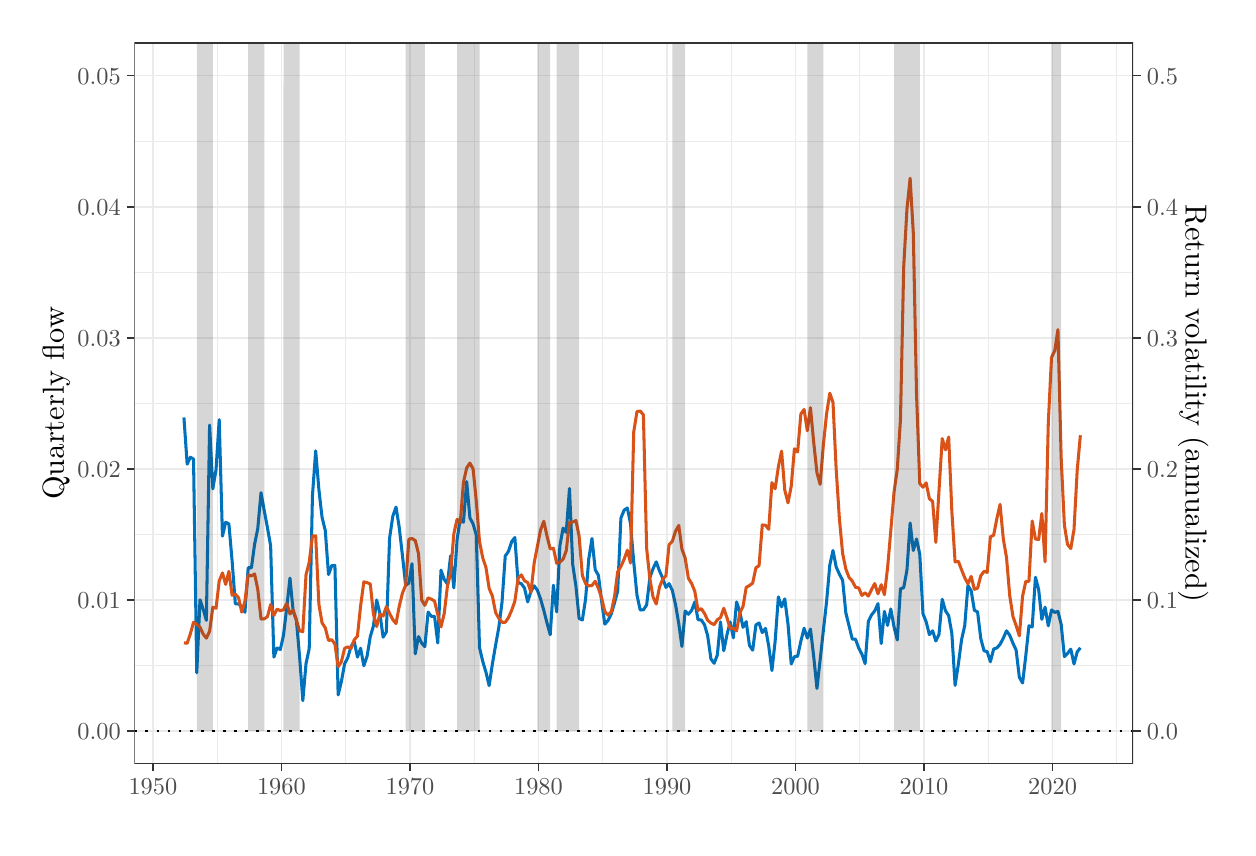
\begin{tikzpicture}[x=1pt,y=1pt]
\definecolor{fillColor}{RGB}{255,255,255}
\path[use as bounding box,fill=fillColor,fill opacity=0.00] (0,0) rectangle (433.62,289.08);
\begin{scope}
\path[clip] (  0.00,  0.00) rectangle (433.62,289.08);
\definecolor{drawColor}{RGB}{255,255,255}
\definecolor{fillColor}{RGB}{255,255,255}

\path[draw=drawColor,line width= 0.6pt,line join=round,line cap=round,fill=fillColor] (  0.00,  0.00) rectangle (433.62,289.08);
\end{scope}
\begin{scope}
\path[clip] ( 38.56, 23.11) rectangle (399.46,283.58);
\definecolor{fillColor}{RGB}{255,255,255}

\path[fill=fillColor] ( 38.56, 23.11) rectangle (399.46,283.58);
\definecolor{drawColor}{gray}{0.92}

\path[draw=drawColor,line width= 0.3pt,line join=round] ( 38.56, 58.63) --
	(399.46, 58.63);

\path[draw=drawColor,line width= 0.3pt,line join=round] ( 38.56,105.99) --
	(399.46,105.99);

\path[draw=drawColor,line width= 0.3pt,line join=round] ( 38.56,153.34) --
	(399.46,153.34);

\path[draw=drawColor,line width= 0.3pt,line join=round] ( 38.56,200.70) --
	(399.46,200.70);

\path[draw=drawColor,line width= 0.3pt,line join=round] ( 38.56,248.06) --
	(399.46,248.06);

\path[draw=drawColor,line width= 0.3pt,line join=round] ( 68.46, 23.11) --
	( 68.46,283.58);

\path[draw=drawColor,line width= 0.3pt,line join=round] (114.91, 23.11) --
	(114.91,283.58);

\path[draw=drawColor,line width= 0.3pt,line join=round] (161.35, 23.11) --
	(161.35,283.58);

\path[draw=drawColor,line width= 0.3pt,line join=round] (207.79, 23.11) --
	(207.79,283.58);

\path[draw=drawColor,line width= 0.3pt,line join=round] (254.24, 23.11) --
	(254.24,283.58);

\path[draw=drawColor,line width= 0.3pt,line join=round] (300.68, 23.11) --
	(300.68,283.58);

\path[draw=drawColor,line width= 0.3pt,line join=round] (347.13, 23.11) --
	(347.13,283.58);

\path[draw=drawColor,line width= 0.3pt,line join=round] (393.57, 23.11) --
	(393.57,283.58);

\path[draw=drawColor,line width= 0.6pt,line join=round] ( 38.56, 34.95) --
	(399.46, 34.95);

\path[draw=drawColor,line width= 0.6pt,line join=round] ( 38.56, 82.31) --
	(399.46, 82.31);

\path[draw=drawColor,line width= 0.6pt,line join=round] ( 38.56,129.67) --
	(399.46,129.67);

\path[draw=drawColor,line width= 0.6pt,line join=round] ( 38.56,177.02) --
	(399.46,177.02);

\path[draw=drawColor,line width= 0.6pt,line join=round] ( 38.56,224.38) --
	(399.46,224.38);

\path[draw=drawColor,line width= 0.6pt,line join=round] ( 38.56,271.74) --
	(399.46,271.74);

\path[draw=drawColor,line width= 0.6pt,line join=round] ( 45.24, 23.11) --
	( 45.24,283.58);

\path[draw=drawColor,line width= 0.6pt,line join=round] ( 91.68, 23.11) --
	( 91.68,283.58);

\path[draw=drawColor,line width= 0.6pt,line join=round] (138.13, 23.11) --
	(138.13,283.58);

\path[draw=drawColor,line width= 0.6pt,line join=round] (184.57, 23.11) --
	(184.57,283.58);

\path[draw=drawColor,line width= 0.6pt,line join=round] (231.02, 23.11) --
	(231.02,283.58);

\path[draw=drawColor,line width= 0.6pt,line join=round] (277.46, 23.11) --
	(277.46,283.58);

\path[draw=drawColor,line width= 0.6pt,line join=round] (323.91, 23.11) --
	(323.91,283.58);

\path[draw=drawColor,line width= 0.6pt,line join=round] (370.35, 23.11) --
	(370.35,283.58);
\definecolor{drawColor}{RGB}{0,114,189}

\path[draw=drawColor,line width= 1.1pt,line join=round] ( 56.46,148.23) --
	( 57.63,131.35) --
	( 58.78,133.87) --
	( 59.93,133.20) --
	( 61.10, 55.94) --
	( 62.27, 82.35) --
	( 63.43, 78.92) --
	( 64.57, 74.89) --
	( 65.74,145.46) --
	( 66.91,122.40) --
	( 68.07,129.42) --
	( 69.21,147.43) --
	( 70.38,105.35) --
	( 71.55,110.38) --
	( 72.71,109.76) --
	( 73.87, 96.40) --
	( 75.04, 80.86) --
	( 76.20, 80.88) --
	( 77.36, 79.88) --
	( 78.51, 77.82) --
	( 79.68, 93.93) --
	( 80.85, 93.90) --
	( 82.00,102.42) --
	( 83.15,108.14) --
	( 84.32,121.04) --
	( 85.49,114.52) --
	( 86.64,108.37) --
	( 87.79,101.91) --
	( 88.96, 61.63) --
	( 90.13, 64.95) --
	( 91.29, 64.36) --
	( 92.44, 69.56) --
	( 93.61, 79.49) --
	( 94.78, 90.18) --
	( 95.94, 78.14) --
	( 97.08, 75.12) --
	( 98.25, 61.92) --
	( 99.42, 45.90) --
	(100.58, 59.30) --
	(101.73, 64.67) --
	(102.90,119.95) --
	(104.07,136.18) --
	(105.22,122.28) --
	(106.37,112.15) --
	(107.54,107.36) --
	(108.71, 91.45) --
	(109.86, 94.67) --
	(111.02, 94.74) --
	(112.19, 47.96) --
	(113.36, 52.82) --
	(114.52, 59.22) --
	(115.66, 61.39) --
	(116.83, 65.47) --
	(118.00, 67.32) --
	(119.16, 61.64) --
	(120.30, 64.84) --
	(121.47, 58.49) --
	(122.64, 61.94) --
	(123.80, 68.99) --
	(124.94, 72.90) --
	(126.11, 82.27) --
	(127.28, 77.37) --
	(128.44, 68.83) --
	(129.60, 70.71) --
	(130.77,104.58) --
	(131.94,112.55) --
	(133.10,115.85) --
	(134.24,108.68) --
	(135.41, 98.46) --
	(136.58, 87.58) --
	(137.74, 88.39) --
	(138.88, 95.39) --
	(140.05, 62.80) --
	(141.22, 69.07) --
	(142.38, 66.67) --
	(143.52, 65.38) --
	(144.69, 77.91) --
	(145.86, 76.38) --
	(147.02, 76.35) --
	(148.18, 66.75) --
	(149.35, 93.06) --
	(150.52, 89.72) --
	(151.67, 88.05) --
	(152.82, 98.25) --
	(153.99, 86.66) --
	(155.16,104.07) --
	(156.31,111.69) --
	(157.46,110.35) --
	(158.63,125.07) --
	(159.80,111.97) --
	(160.96,109.72) --
	(162.10,105.75) --
	(163.27, 65.08) --
	(164.44, 60.06) --
	(165.60, 56.18) --
	(166.75, 51.32) --
	(167.92, 59.16) --
	(169.09, 65.97) --
	(170.25, 72.39) --
	(171.40, 81.43) --
	(172.57, 98.18) --
	(173.73, 99.82) --
	(174.89,103.34) --
	(176.04,104.86) --
	(177.21, 88.53) --
	(178.38, 88.19) --
	(179.53, 86.58) --
	(180.68, 81.58) --
	(181.85, 85.38) --
	(183.02, 87.39) --
	(184.17, 85.81) --
	(185.33, 82.66) --
	(186.50, 78.55) --
	(187.67, 73.90) --
	(188.83, 69.71) --
	(189.97, 87.62) --
	(191.14, 77.98) --
	(192.31,101.82) --
	(193.47,108.25) --
	(194.61,106.69) --
	(195.78,122.58) --
	(196.95, 95.08) --
	(198.11, 87.28) --
	(199.26, 75.61) --
	(200.43, 75.03) --
	(201.60, 82.62) --
	(202.75, 97.16) --
	(203.91,104.49) --
	(205.08, 93.21) --
	(206.25, 91.12) --
	(207.41, 81.73) --
	(208.55, 73.54) --
	(209.72, 74.87) --
	(210.89, 77.29) --
	(212.05, 81.20) --
	(213.19, 85.43) --
	(214.36,111.86) --
	(215.53,114.75) --
	(216.69,115.53) --
	(217.83,109.83) --
	(219.00, 95.94) --
	(220.17, 84.02) --
	(221.33, 78.66) --
	(222.49, 78.71) --
	(223.66, 80.48) --
	(224.83, 90.41) --
	(225.98, 93.59) --
	(227.13, 96.06) --
	(228.30, 92.78) --
	(229.47, 90.17) --
	(230.63, 86.82) --
	(231.77, 88.18) --
	(232.94, 85.72) --
	(234.11, 80.54) --
	(235.27, 73.75) --
	(236.41, 65.47) --
	(237.58, 78.29) --
	(238.75, 77.12) --
	(239.91, 78.51) --
	(241.06, 81.54) --
	(242.23, 75.15) --
	(243.40, 75.05) --
	(244.56, 73.36) --
	(245.71, 69.40) --
	(246.88, 61.00) --
	(248.05, 59.40) --
	(249.20, 62.36) --
	(250.35, 74.36) --
	(251.52, 63.92) --
	(252.69, 69.71) --
	(253.84, 74.34) --
	(254.99, 68.59) --
	(256.16, 81.58) --
	(257.33, 77.98) --
	(258.49, 72.40) --
	(259.64, 74.44) --
	(260.81, 65.85) --
	(261.98, 64.13) --
	(263.14, 73.26) --
	(264.28, 73.98) --
	(265.45, 70.49) --
	(266.62, 72.03) --
	(267.78, 65.60) --
	(268.93, 56.78) --
	(270.10, 67.42) --
	(271.26, 83.40) --
	(272.42, 79.82) --
	(273.57, 82.68) --
	(274.74, 73.61) --
	(275.91, 59.14) --
	(277.06, 61.79) --
	(278.22, 61.96) --
	(279.39, 67.39) --
	(280.56, 72.08) --
	(281.72, 68.52) --
	(282.86, 71.76) --
	(284.03, 61.85) --
	(285.20, 50.31) --
	(286.36, 60.66) --
	(287.50, 71.10) --
	(288.67, 81.53) --
	(289.84, 94.91) --
	(291.00,100.15) --
	(292.14, 94.25) --
	(293.31, 91.60) --
	(294.48, 89.41) --
	(295.64, 77.63) --
	(296.80, 72.95) --
	(297.97, 68.14) --
	(299.14, 68.10) --
	(300.30, 64.88) --
	(301.44, 62.72) --
	(302.61, 59.25) --
	(303.78, 74.55) --
	(304.94, 76.89) --
	(306.08, 78.32) --
	(307.25, 80.95) --
	(308.42, 66.52) --
	(309.58, 78.17) --
	(310.72, 73.09) --
	(311.89, 79.03) --
	(313.06, 72.53) --
	(314.22, 67.82) --
	(315.38, 86.32) --
	(316.55, 86.73) --
	(317.72, 93.05) --
	(318.87,110.10) --
	(320.02,100.16) --
	(321.19,104.32) --
	(322.36, 98.80) --
	(323.51, 77.33) --
	(324.66, 74.39) --
	(325.83, 69.74) --
	(327.00, 71.15) --
	(328.16, 67.46) --
	(329.30, 69.85) --
	(330.47, 82.54) --
	(331.64, 78.38) --
	(332.80, 76.60) --
	(333.95, 70.19) --
	(335.12, 51.40) --
	(336.29, 59.02) --
	(337.45, 67.88) --
	(338.60, 72.98) --
	(339.76, 87.52) --
	(340.93, 85.63) --
	(342.09, 78.53) --
	(343.24, 77.98) --
	(344.41, 68.27) --
	(345.58, 63.96) --
	(346.73, 63.57) --
	(347.88, 59.95) --
	(349.05, 64.56) --
	(350.22, 64.98) --
	(351.37, 66.23) --
	(352.53, 68.46) --
	(353.70, 71.13) --
	(354.87, 69.50) --
	(356.03, 66.65) --
	(357.17, 64.18) --
	(358.34, 54.32) --
	(359.51, 52.28) --
	(360.67, 62.19) --
	(361.81, 72.94) --
	(362.98, 72.51) --
	(364.15, 90.49) --
	(365.31, 86.11) --
	(366.46, 75.25) --
	(367.63, 79.68) --
	(368.80, 72.94) --
	(369.95, 78.69) --
	(371.11, 77.80) --
	(372.28, 78.14) --
	(373.45, 73.51) --
	(374.61, 61.79) --
	(375.75, 62.97) --
	(376.92, 64.51) --
	(378.09, 59.15) --
	(379.25, 63.53) --
	(380.39, 65.00);
\definecolor{drawColor}{RGB}{217,83,25}

\path[draw=drawColor,line width= 1.1pt,line join=round] ( 56.46, 66.79) --
	( 57.63, 66.63) --
	( 58.78, 70.01) --
	( 59.93, 74.24) --
	( 61.10, 73.46) --
	( 62.27, 72.45) --
	( 63.43, 69.92) --
	( 64.57, 68.49) --
	( 65.74, 70.98) --
	( 66.91, 79.67) --
	( 68.07, 79.29) --
	( 69.21, 89.14) --
	( 70.38, 92.05) --
	( 71.55, 87.89) --
	( 72.71, 92.64) --
	( 73.87, 84.00) --
	( 75.04, 84.38) --
	( 76.20, 83.09) --
	( 77.36, 77.90) --
	( 78.51, 81.82) --
	( 79.68, 91.35) --
	( 80.85, 90.96) --
	( 82.00, 91.70) --
	( 83.15, 86.06) --
	( 84.32, 75.39) --
	( 85.49, 75.45) --
	( 86.64, 76.25) --
	( 87.79, 80.63) --
	( 88.96, 76.66) --
	( 90.13, 78.98) --
	( 91.29, 78.40) --
	( 92.44, 78.75) --
	( 93.61, 81.06) --
	( 94.78, 77.21) --
	( 95.94, 78.67) --
	( 97.08, 74.98) --
	( 98.25, 71.08) --
	( 99.42, 70.85) --
	(100.58, 91.38) --
	(101.73, 95.84) --
	(102.90,105.40) --
	(104.07,105.47) --
	(105.22, 80.76) --
	(106.37, 74.04) --
	(107.54, 72.19) --
	(108.71, 67.64) --
	(109.86, 67.92) --
	(111.02, 66.37) --
	(112.19, 58.11) --
	(113.36, 59.95) --
	(114.52, 64.81) --
	(115.66, 65.33) --
	(116.83, 64.75) --
	(118.00, 67.89) --
	(119.16, 69.21) --
	(120.30, 80.08) --
	(121.47, 88.83) --
	(122.64, 88.53) --
	(123.80, 88.06) --
	(124.94, 77.14) --
	(126.11, 72.68) --
	(127.28, 77.15) --
	(128.44, 76.49) --
	(129.60, 79.88) --
	(130.77, 77.45) --
	(131.94, 75.16) --
	(133.10, 73.75) --
	(134.24, 79.88) --
	(135.41, 84.72) --
	(136.58, 87.65) --
	(137.74,104.26) --
	(138.88,104.48) --
	(140.05,103.77) --
	(141.22, 99.06) --
	(142.38, 82.25) --
	(143.52, 80.33) --
	(144.69, 83.03) --
	(145.86, 82.59) --
	(147.02, 81.88) --
	(148.18, 77.04) --
	(149.35, 72.54) --
	(150.52, 77.41) --
	(151.67, 87.21) --
	(152.82, 91.97) --
	(153.99,106.16) --
	(155.16,111.43) --
	(156.31,110.05) --
	(157.46,124.74) --
	(158.63,130.00) --
	(159.80,131.73) --
	(160.96,129.62) --
	(162.10,118.01) --
	(163.27,103.44) --
	(164.44, 97.48) --
	(165.60, 93.99) --
	(166.75, 86.47) --
	(167.92, 83.69) --
	(169.09, 77.73) --
	(170.25, 75.65) --
	(171.40, 74.24) --
	(172.57, 74.19) --
	(173.73, 75.89) --
	(174.89, 78.55) --
	(176.04, 81.81) --
	(177.21, 90.12) --
	(178.38, 91.36) --
	(179.53, 89.21) --
	(180.68, 88.59) --
	(181.85, 85.09) --
	(183.02, 95.64) --
	(184.17,101.64) --
	(185.33,107.56) --
	(186.50,110.74) --
	(187.67,105.31) --
	(188.83,100.72) --
	(189.97,100.99) --
	(191.14, 95.56) --
	(192.31, 95.98) --
	(193.47, 97.02) --
	(194.61,100.06) --
	(195.78,110.33) --
	(196.95,110.46) --
	(198.11,110.97) --
	(199.26,105.40) --
	(200.43, 91.12) --
	(201.60, 88.19) --
	(202.75, 87.35) --
	(203.91, 87.51) --
	(205.08, 89.04) --
	(206.25, 86.42) --
	(207.41, 82.96) --
	(208.55, 78.08) --
	(209.72, 76.80) --
	(210.89, 78.06) --
	(212.05, 83.47) --
	(213.19, 92.44) --
	(214.36, 94.36) --
	(215.53, 97.03) --
	(216.69,100.26) --
	(217.83, 95.62) --
	(219.00,143.01) --
	(220.17,150.37) --
	(221.33,150.55) --
	(222.49,149.16) --
	(223.66,100.92) --
	(224.83, 89.92) --
	(225.98, 83.33) --
	(227.13, 80.82) --
	(228.30, 86.93) --
	(229.47, 89.78) --
	(230.63, 91.01) --
	(231.77,102.25) --
	(232.94,103.50) --
	(234.11,107.13) --
	(235.27,109.20) --
	(236.41,100.63) --
	(237.58, 97.48) --
	(238.75, 90.11) --
	(239.91, 88.22) --
	(241.06, 85.41) --
	(242.23, 78.50) --
	(243.40, 79.15) --
	(244.56, 77.44) --
	(245.71, 74.96) --
	(246.88, 73.94) --
	(248.05, 73.35) --
	(249.20, 75.13) --
	(250.35, 75.89) --
	(251.52, 79.28) --
	(252.69, 75.87) --
	(253.84, 71.99) --
	(254.99, 72.13) --
	(256.16, 71.11) --
	(257.33, 77.64) --
	(258.49, 79.92) --
	(259.64, 86.85) --
	(260.81, 87.49) --
	(261.98, 88.38) --
	(263.14, 93.90) --
	(264.28, 94.67) --
	(265.45,109.38) --
	(266.62,109.28) --
	(267.78,107.81) --
	(268.93,124.69) --
	(270.10,122.46) --
	(271.26,130.41) --
	(272.42,136.06) --
	(273.57,121.99) --
	(274.74,117.36) --
	(275.91,123.39) --
	(277.06,136.92) --
	(278.22,135.75) --
	(279.39,149.50) --
	(280.56,151.12) --
	(281.72,143.42) --
	(282.86,151.77) --
	(284.03,139.22) --
	(285.20,128.25) --
	(286.36,124.05) --
	(287.50,138.10) --
	(288.67,149.44) --
	(289.84,156.99) --
	(291.00,153.66) --
	(292.14,129.69) --
	(293.31,111.68) --
	(294.48, 99.09) --
	(295.64, 93.48) --
	(296.80, 90.43) --
	(297.97, 89.10) --
	(299.14, 86.85) --
	(300.30, 86.64) --
	(301.44, 83.92) --
	(302.61, 84.86) --
	(303.78, 83.68) --
	(304.94, 86.08) --
	(306.08, 88.22) --
	(307.25, 84.50) --
	(308.42, 87.78) --
	(309.58, 84.18) --
	(310.72, 93.87) --
	(311.89,107.32) --
	(313.06,121.37) --
	(314.22,129.43) --
	(315.38,147.40) --
	(316.55,202.67) --
	(317.72,223.49) --
	(318.87,234.68) --
	(320.02,214.83) --
	(321.19,156.57) --
	(322.36,124.36) --
	(323.51,123.02) --
	(324.66,124.58) --
	(325.83,118.87) --
	(327.00,117.90) --
	(328.16,103.08) --
	(329.30,121.67) --
	(330.47,140.60) --
	(331.64,136.53) --
	(332.80,141.16) --
	(333.95,114.22) --
	(335.12, 96.02) --
	(336.29, 96.26) --
	(337.45, 93.20) --
	(338.60, 90.33) --
	(339.76, 88.12) --
	(340.93, 90.80) --
	(342.09, 86.12) --
	(343.24, 86.53) --
	(344.41, 91.01) --
	(345.58, 92.63) --
	(346.73, 92.25) --
	(347.88,105.13) --
	(349.05,105.65) --
	(350.22,111.74) --
	(351.37,116.80) --
	(352.53,104.47) --
	(353.70, 97.60) --
	(354.87, 83.78) --
	(356.03, 76.28) --
	(357.17, 73.03) --
	(358.34, 69.30) --
	(359.51, 83.68) --
	(360.67, 89.00) --
	(361.81, 89.02) --
	(362.98,110.84) --
	(364.15,104.33) --
	(365.31,104.12) --
	(366.46,113.54) --
	(367.63, 96.07) --
	(368.80,146.28) --
	(369.95,169.89) --
	(371.11,172.32) --
	(372.28,179.97) --
	(373.45,133.71) --
	(374.61,109.32) --
	(375.75,102.33) --
	(376.92,100.85) --
	(378.09,107.76) --
	(379.25,129.21) --
	(380.39,141.80);
\definecolor{fillColor}{RGB}{51,51,51}

\path[fill=fillColor,fill opacity=0.20] ( 55.29, 34.95) --
	( 55.61, 34.95) --
	( 56.13, 34.95) --
	( 56.46, 34.95) --
	( 56.78, 34.95) --
	( 57.30, 34.95) --
	( 57.63, 34.95) --
	( 57.95, 34.95) --
	( 58.46, 34.95) --
	( 58.78, 34.95) --
	( 59.11, 34.95) --
	( 59.60, 34.95) --
	( 59.93, 34.95) --
	( 60.26, 34.95) --
	( 60.77, 34.95) --
	( 61.10, 34.95) --
	( 61.10,2023.56) --
	( 66.90,2023.56) --
	( 66.91, 34.95) --
	( 67.24, 34.95) --
	( 67.74, 34.95) --
	( 68.07, 34.95) --
	( 68.39, 34.95) --
	( 68.88, 34.95) --
	( 69.21, 34.95) --
	( 69.54, 34.95) --
	( 70.05, 34.95) --
	( 70.38, 34.95) --
	( 70.71, 34.95) --
	( 71.22, 34.95) --
	( 71.55, 34.95) --
	( 71.88, 34.95) --
	( 72.38, 34.95) --
	( 72.71, 34.95) --
	( 73.04, 34.95) --
	( 73.54, 34.95) --
	( 73.87, 34.95) --
	( 74.19, 34.95) --
	( 74.71, 34.95) --
	( 75.04, 34.95) --
	( 75.36, 34.95) --
	( 75.88, 34.95) --
	( 76.20, 34.95) --
	( 76.53, 34.95) --
	( 77.03, 34.95) --
	( 77.36, 34.95) --
	( 77.69, 34.95) --
	( 78.18, 34.95) --
	( 78.51, 34.95) --
	( 78.83, 34.95) --
	( 79.35, 34.95) --
	( 79.68, 34.95) --
	( 79.68,2023.56) --
	( 85.48,2023.56) --
	( 85.49, 34.95) --
	( 85.81, 34.95) --
	( 86.32, 34.95) --
	( 86.64, 34.95) --
	( 86.97, 34.95) --
	( 87.46, 34.95) --
	( 87.79, 34.95) --
	( 88.12, 34.95) --
	( 88.63, 34.95) --
	( 88.96, 34.95) --
	( 89.29, 34.95) --
	( 89.80, 34.95) --
	( 90.13, 34.95) --
	( 90.46, 34.95) --
	( 90.96, 34.95) --
	( 91.29, 34.95) --
	( 91.61, 34.95) --
	( 92.12, 34.95) --
	( 92.44, 34.95) --
	( 92.45,2023.56) --
	( 98.25,2023.56) --
	( 98.25, 34.95) --
	( 98.58, 34.95) --
	( 99.10, 34.95) --
	( 99.42, 34.95) --
	( 99.75, 34.95) --
	(100.25, 34.95) --
	(100.58, 34.95) --
	(100.91, 34.95) --
	(101.40, 34.95) --
	(101.73, 34.95) --
	(102.05, 34.95) --
	(102.57, 34.95) --
	(102.90, 34.95) --
	(103.22, 34.95) --
	(103.74, 34.95) --
	(104.07, 34.95) --
	(104.39, 34.95) --
	(104.89, 34.95) --
	(105.22, 34.95) --
	(105.55, 34.95) --
	(106.04, 34.95) --
	(106.37, 34.95) --
	(106.69, 34.95) --
	(107.21, 34.95) --
	(107.54, 34.95) --
	(107.86, 34.95) --
	(108.38, 34.95) --
	(108.71, 34.95) --
	(109.03, 34.95) --
	(109.54, 34.95) --
	(109.86, 34.95) --
	(110.19, 34.95) --
	(110.69, 34.95) --
	(111.02, 34.95) --
	(111.35, 34.95) --
	(111.86, 34.95) --
	(112.19, 34.95) --
	(112.52, 34.95) --
	(113.03, 34.95) --
	(113.36, 34.95) --
	(113.69, 34.95) --
	(114.19, 34.95) --
	(114.52, 34.95) --
	(114.84, 34.95) --
	(115.33, 34.95) --
	(115.66, 34.95) --
	(115.99, 34.95) --
	(116.50, 34.95) --
	(116.83, 34.95) --
	(117.16, 34.95) --
	(117.67, 34.95) --
	(118.00, 34.95) --
	(118.33, 34.95) --
	(118.83, 34.95) --
	(119.16, 34.95) --
	(119.49, 34.95) --
	(119.98, 34.95) --
	(120.30, 34.95) --
	(120.63, 34.95) --
	(121.15, 34.95) --
	(121.47, 34.95) --
	(121.80, 34.95) --
	(122.32, 34.95) --
	(122.64, 34.95) --
	(122.97, 34.95) --
	(123.47, 34.95) --
	(123.80, 34.95) --
	(124.13, 34.95) --
	(124.62, 34.95) --
	(124.94, 34.95) --
	(125.27, 34.95) --
	(125.79, 34.95) --
	(126.11, 34.95) --
	(126.44, 34.95) --
	(126.96, 34.95) --
	(127.28, 34.95) --
	(127.61, 34.95) --
	(128.11, 34.95) --
	(128.44, 34.95) --
	(128.77, 34.95) --
	(129.27, 34.95) --
	(129.60, 34.95) --
	(129.93, 34.95) --
	(130.44, 34.95) --
	(130.77, 34.95) --
	(131.10, 34.95) --
	(131.61, 34.95) --
	(131.94, 34.95) --
	(132.27, 34.95) --
	(132.77, 34.95) --
	(133.10, 34.95) --
	(133.42, 34.95) --
	(133.91, 34.95) --
	(134.24, 34.95) --
	(134.57, 34.95) --
	(135.08, 34.95) --
	(135.41, 34.95) --
	(135.74, 34.95) --
	(136.25, 34.95) --
	(136.58, 34.95) --
	(136.58,2023.56) --
	(143.52,2023.56) --
	(143.52, 34.95) --
	(143.85, 34.95) --
	(144.36, 34.95) --
	(144.69, 34.95) --
	(145.02, 34.95) --
	(145.53, 34.95) --
	(145.86, 34.95) --
	(146.19, 34.95) --
	(146.69, 34.95) --
	(147.02, 34.95) --
	(147.35, 34.95) --
	(147.85, 34.95) --
	(148.18, 34.95) --
	(148.50, 34.95) --
	(149.02, 34.95) --
	(149.35, 34.95) --
	(149.67, 34.95) --
	(150.19, 34.95) --
	(150.52, 34.95) --
	(150.84, 34.95) --
	(151.35, 34.95) --
	(151.67, 34.95) --
	(152.00, 34.95) --
	(152.49, 34.95) --
	(152.82, 34.95) --
	(153.14, 34.95) --
	(153.66, 34.95) --
	(153.99, 34.95) --
	(154.31, 34.95) --
	(154.83, 34.95) --
	(155.16, 34.95) --
	(155.16,2023.56) --
	(163.26,2023.56) --
	(163.27, 34.95) --
	(163.60, 34.95) --
	(164.11, 34.95) --
	(164.44, 34.95) --
	(164.77, 34.95) --
	(165.27, 34.95) --
	(165.60, 34.95) --
	(165.92, 34.95) --
	(166.43, 34.95) --
	(166.75, 34.95) --
	(167.08, 34.95) --
	(167.60, 34.95) --
	(167.92, 34.95) --
	(168.25, 34.95) --
	(168.77, 34.95) --
	(169.09, 34.95) --
	(169.42, 34.95) --
	(169.92, 34.95) --
	(170.25, 34.95) --
	(170.58, 34.95) --
	(171.07, 34.95) --
	(171.40, 34.95) --
	(171.72, 34.95) --
	(172.24, 34.95) --
	(172.57, 34.95) --
	(172.89, 34.95) --
	(173.41, 34.95) --
	(173.73, 34.95) --
	(174.06, 34.95) --
	(174.56, 34.95) --
	(174.89, 34.95) --
	(175.22, 34.95) --
	(175.71, 34.95) --
	(176.04, 34.95) --
	(176.36, 34.95) --
	(176.88, 34.95) --
	(177.21, 34.95) --
	(177.53, 34.95) --
	(178.05, 34.95) --
	(178.38, 34.95) --
	(178.70, 34.95) --
	(179.21, 34.95) --
	(179.53, 34.95) --
	(179.86, 34.95) --
	(180.35, 34.95) --
	(180.68, 34.95) --
	(181.01, 34.95) --
	(181.52, 34.95) --
	(181.85, 34.95) --
	(182.18, 34.95) --
	(182.69, 34.95) --
	(183.02, 34.95) --
	(183.34, 34.95) --
	(183.85, 34.95) --
	(184.17, 34.95) --
	(184.18,2023.56) --
	(188.82,2023.56) --
	(188.83, 34.95) --
	(189.16, 34.95) --
	(189.65, 34.95) --
	(189.97, 34.95) --
	(190.30, 34.95) --
	(190.82, 34.95) --
	(191.14, 34.95) --
	(191.15,2023.56) --
	(199.25,2023.56) --
	(199.26, 34.95) --
	(199.58, 34.95) --
	(200.10, 34.95) --
	(200.43, 34.95) --
	(200.75, 34.95) --
	(201.27, 34.95) --
	(201.60, 34.95) --
	(201.92, 34.95) --
	(202.42, 34.95) --
	(202.75, 34.95) --
	(203.08, 34.95) --
	(203.58, 34.95) --
	(203.91, 34.95) --
	(204.24, 34.95) --
	(204.75, 34.95) --
	(205.08, 34.95) --
	(205.41, 34.95) --
	(205.92, 34.95) --
	(206.25, 34.95) --
	(206.58, 34.95) --
	(207.08, 34.95) --
	(207.41, 34.95) --
	(207.73, 34.95) --
	(208.22, 34.95) --
	(208.55, 34.95) --
	(208.88, 34.95) --
	(209.39, 34.95) --
	(209.72, 34.95) --
	(210.05, 34.95) --
	(210.56, 34.95) --
	(210.89, 34.95) --
	(211.22, 34.95) --
	(211.72, 34.95) --
	(212.05, 34.95) --
	(212.38, 34.95) --
	(212.86, 34.95) --
	(213.19, 34.95) --
	(213.52, 34.95) --
	(214.03, 34.95) --
	(214.36, 34.95) --
	(214.69, 34.95) --
	(215.20, 34.95) --
	(215.53, 34.95) --
	(215.86, 34.95) --
	(216.36, 34.95) --
	(216.69, 34.95) --
	(217.02, 34.95) --
	(217.51, 34.95) --
	(217.83, 34.95) --
	(218.16, 34.95) --
	(218.68, 34.95) --
	(219.00, 34.95) --
	(219.33, 34.95) --
	(219.85, 34.95) --
	(220.17, 34.95) --
	(220.50, 34.95) --
	(221.00, 34.95) --
	(221.33, 34.95) --
	(221.66, 34.95) --
	(222.16, 34.95) --
	(222.49, 34.95) --
	(222.81, 34.95) --
	(223.33, 34.95) --
	(223.66, 34.95) --
	(223.98, 34.95) --
	(224.50, 34.95) --
	(224.83, 34.95) --
	(225.15, 34.95) --
	(225.66, 34.95) --
	(225.98, 34.95) --
	(226.31, 34.95) --
	(226.80, 34.95) --
	(227.13, 34.95) --
	(227.46, 34.95) --
	(227.97, 34.95) --
	(228.30, 34.95) --
	(228.63, 34.95) --
	(229.14, 34.95) --
	(229.47, 34.95) --
	(229.80, 34.95) --
	(230.30, 34.95) --
	(230.63, 34.95) --
	(230.95, 34.95) --
	(231.44, 34.95) --
	(231.77, 34.95) --
	(232.10, 34.95) --
	(232.61, 34.95) --
	(232.94, 34.95) --
	(232.94,2023.56) --
	(237.58,2023.56) --
	(237.58, 34.95) --
	(237.91, 34.95) --
	(238.42, 34.95) --
	(238.75, 34.95) --
	(239.08, 34.95) --
	(239.58, 34.95) --
	(239.91, 34.95) --
	(240.24, 34.95) --
	(240.74, 34.95) --
	(241.06, 34.95) --
	(241.39, 34.95) --
	(241.91, 34.95) --
	(242.23, 34.95) --
	(242.56, 34.95) --
	(243.08, 34.95) --
	(243.40, 34.95) --
	(243.73, 34.95) --
	(244.23, 34.95) --
	(244.56, 34.95) --
	(244.89, 34.95) --
	(245.38, 34.95) --
	(245.71, 34.95) --
	(246.03, 34.95) --
	(246.55, 34.95) --
	(246.88, 34.95) --
	(247.20, 34.95) --
	(247.72, 34.95) --
	(248.05, 34.95) --
	(248.37, 34.95) --
	(248.88, 34.95) --
	(249.20, 34.95) --
	(249.53, 34.95) --
	(250.02, 34.95) --
	(250.35, 34.95) --
	(250.67, 34.95) --
	(251.19, 34.95) --
	(251.52, 34.95) --
	(251.84, 34.95) --
	(252.36, 34.95) --
	(252.69, 34.95) --
	(253.01, 34.95) --
	(253.52, 34.95) --
	(253.84, 34.95) --
	(254.17, 34.95) --
	(254.66, 34.95) --
	(254.99, 34.95) --
	(255.32, 34.95) --
	(255.83, 34.95) --
	(256.16, 34.95) --
	(256.49, 34.95) --
	(257.00, 34.95) --
	(257.33, 34.95) --
	(257.66, 34.95) --
	(258.16, 34.95) --
	(258.49, 34.95) --
	(258.81, 34.95) --
	(259.32, 34.95) --
	(259.64, 34.95) --
	(259.97, 34.95) --
	(260.49, 34.95) --
	(260.81, 34.95) --
	(261.14, 34.95) --
	(261.66, 34.95) --
	(261.98, 34.95) --
	(262.31, 34.95) --
	(262.81, 34.95) --
	(263.14, 34.95) --
	(263.47, 34.95) --
	(263.96, 34.95) --
	(264.28, 34.95) --
	(264.61, 34.95) --
	(265.13, 34.95) --
	(265.45, 34.95) --
	(265.78, 34.95) --
	(266.30, 34.95) --
	(266.62, 34.95) --
	(266.95, 34.95) --
	(267.45, 34.95) --
	(267.78, 34.95) --
	(268.11, 34.95) --
	(268.60, 34.95) --
	(268.93, 34.95) --
	(269.25, 34.95) --
	(269.77, 34.95) --
	(270.10, 34.95) --
	(270.42, 34.95) --
	(270.94, 34.95) --
	(271.26, 34.95) --
	(271.59, 34.95) --
	(272.09, 34.95) --
	(272.42, 34.95) --
	(272.75, 34.95) --
	(273.24, 34.95) --
	(273.57, 34.95) --
	(273.89, 34.95) --
	(274.41, 34.95) --
	(274.74, 34.95) --
	(275.06, 34.95) --
	(275.58, 34.95) --
	(275.91, 34.95) --
	(276.23, 34.95) --
	(276.74, 34.95) --
	(277.06, 34.95) --
	(277.39, 34.95) --
	(277.89, 34.95) --
	(278.22, 34.95) --
	(278.55, 34.95) --
	(279.06, 34.95) --
	(279.39, 34.95) --
	(279.72, 34.95) --
	(280.23, 34.95) --
	(280.56, 34.95) --
	(280.89, 34.95) --
	(281.39, 34.95) --
	(281.72, 34.95) --
	(281.72,2023.56) --
	(287.50,2023.56) --
	(287.50, 34.95) --
	(287.83, 34.95) --
	(288.35, 34.95) --
	(288.67, 34.95) --
	(289.00, 34.95) --
	(289.52, 34.95) --
	(289.84, 34.95) --
	(290.17, 34.95) --
	(290.67, 34.95) --
	(291.00, 34.95) --
	(291.33, 34.95) --
	(291.82, 34.95) --
	(292.14, 34.95) --
	(292.47, 34.95) --
	(292.99, 34.95) --
	(293.31, 34.95) --
	(293.64, 34.95) --
	(294.16, 34.95) --
	(294.48, 34.95) --
	(294.81, 34.95) --
	(295.31, 34.95) --
	(295.64, 34.95) --
	(295.97, 34.95) --
	(296.47, 34.95) --
	(296.80, 34.95) --
	(297.13, 34.95) --
	(297.64, 34.95) --
	(297.97, 34.95) --
	(298.30, 34.95) --
	(298.81, 34.95) --
	(299.14, 34.95) --
	(299.47, 34.95) --
	(299.97, 34.95) --
	(300.30, 34.95) --
	(300.62, 34.95) --
	(301.11, 34.95) --
	(301.44, 34.95) --
	(301.77, 34.95) --
	(302.28, 34.95) --
	(302.61, 34.95) --
	(302.94, 34.95) --
	(303.45, 34.95) --
	(303.78, 34.95) --
	(304.11, 34.95) --
	(304.61, 34.95) --
	(304.94, 34.95) --
	(305.26, 34.95) --
	(305.75, 34.95) --
	(306.08, 34.95) --
	(306.41, 34.95) --
	(306.92, 34.95) --
	(307.25, 34.95) --
	(307.58, 34.95) --
	(308.09, 34.95) --
	(308.42, 34.95) --
	(308.75, 34.95) --
	(309.25, 34.95) --
	(309.58, 34.95) --
	(309.91, 34.95) --
	(310.39, 34.95) --
	(310.72, 34.95) --
	(311.05, 34.95) --
	(311.56, 34.95) --
	(311.89, 34.95) --
	(312.22, 34.95) --
	(312.73, 34.95) --
	(313.06, 34.95) --
	(313.07,2023.56) --
	(322.35,2023.56) --
	(322.36, 34.95) --
	(322.68, 34.95) --
	(323.19, 34.95) --
	(323.51, 34.95) --
	(323.84, 34.95) --
	(324.33, 34.95) --
	(324.66, 34.95) --
	(324.99, 34.95) --
	(325.50, 34.95) --
	(325.83, 34.95) --
	(326.16, 34.95) --
	(326.67, 34.95) --
	(327.00, 34.95) --
	(327.33, 34.95) --
	(327.83, 34.95) --
	(328.16, 34.95) --
	(328.48, 34.95) --
	(328.97, 34.95) --
	(329.30, 34.95) --
	(329.63, 34.95) --
	(330.14, 34.95) --
	(330.47, 34.95) --
	(330.80, 34.95) --
	(331.31, 34.95) --
	(331.64, 34.95) --
	(331.97, 34.95) --
	(332.47, 34.95) --
	(332.80, 34.95) --
	(333.12, 34.95) --
	(333.63, 34.95) --
	(333.95, 34.95) --
	(334.28, 34.95) --
	(334.80, 34.95) --
	(335.12, 34.95) --
	(335.45, 34.95) --
	(335.97, 34.95) --
	(336.29, 34.95) --
	(336.62, 34.95) --
	(337.12, 34.95) --
	(337.45, 34.95) --
	(337.78, 34.95) --
	(338.27, 34.95) --
	(338.60, 34.95) --
	(338.92, 34.95) --
	(339.44, 34.95) --
	(339.76, 34.95) --
	(340.09, 34.95) --
	(340.61, 34.95) --
	(340.93, 34.95) --
	(341.26, 34.95) --
	(341.76, 34.95) --
	(342.09, 34.95) --
	(342.42, 34.95) --
	(342.91, 34.95) --
	(343.24, 34.95) --
	(343.56, 34.95) --
	(344.08, 34.95) --
	(344.41, 34.95) --
	(344.73, 34.95) --
	(345.25, 34.95) --
	(345.58, 34.95) --
	(345.90, 34.95) --
	(346.41, 34.95) --
	(346.73, 34.95) --
	(347.06, 34.95) --
	(347.55, 34.95) --
	(347.88, 34.95) --
	(348.21, 34.95) --
	(348.72, 34.95) --
	(349.05, 34.95) --
	(349.37, 34.95) --
	(349.89, 34.95) --
	(350.22, 34.95) --
	(350.54, 34.95) --
	(351.05, 34.95) --
	(351.37, 34.95) --
	(351.70, 34.95) --
	(352.20, 34.95) --
	(352.53, 34.95) --
	(352.86, 34.95) --
	(353.37, 34.95) --
	(353.70, 34.95) --
	(354.03, 34.95) --
	(354.54, 34.95) --
	(354.87, 34.95) --
	(355.20, 34.95) --
	(355.70, 34.95) --
	(356.03, 34.95) --
	(356.36, 34.95) --
	(356.85, 34.95) --
	(357.17, 34.95) --
	(357.50, 34.95) --
	(358.02, 34.95) --
	(358.34, 34.95) --
	(358.67, 34.95) --
	(359.19, 34.95) --
	(359.51, 34.95) --
	(359.84, 34.95) --
	(360.34, 34.95) --
	(360.67, 34.95) --
	(361.00, 34.95) --
	(361.49, 34.95) --
	(361.81, 34.95) --
	(362.14, 34.95) --
	(362.66, 34.95) --
	(362.98, 34.95) --
	(363.31, 34.95) --
	(363.83, 34.95) --
	(364.15, 34.95) --
	(364.48, 34.95) --
	(364.98, 34.95) --
	(365.31, 34.95) --
	(365.64, 34.95) --
	(366.13, 34.95) --
	(366.46, 34.95) --
	(366.78, 34.95) --
	(367.30, 34.95) --
	(367.63, 34.95) --
	(367.95, 34.95) --
	(368.47, 34.95) --
	(368.80, 34.95) --
	(369.12, 34.95) --
	(369.62, 34.95) --
	(369.95, 34.95) --
	(369.96,2023.56) --
	(373.44,2023.56) --
	(373.45, 34.95) --
	(373.78, 34.95) --
	(374.28, 34.95) --
	(374.61, 34.95) --
	(374.93, 34.95) --
	(375.42, 34.95) --
	(375.75, 34.95) --
	(376.08, 34.95) --
	(376.59, 34.95) --
	(376.92, 34.95) --
	(377.25, 34.95) --
	(377.76, 34.95) --
	(378.09, 34.95) --
	(378.42, 34.95) --
	(378.92, 34.95) --
	(379.25, 34.95) --
	(379.57, 34.95) --
	(380.06, 34.95) --
	(380.39, 34.95) --
	(380.72, 34.95) --
	(381.23, 34.95) --
	(381.56, 34.95) --
	(381.89, 34.95) --
	(382.40, 34.95) --
	(382.73, 34.95) --
	(383.06, 34.95) --
	(382.73, 34.95) --
	(382.40, 34.95) --
	(381.89, 34.95) --
	(381.56, 34.95) --
	(381.23, 34.95) --
	(380.72, 34.95) --
	(380.39, 34.95) --
	(380.06, 34.95) --
	(379.57, 34.95) --
	(379.25, 34.95) --
	(378.92, 34.95) --
	(378.42, 34.95) --
	(378.09, 34.95) --
	(377.76, 34.95) --
	(377.25, 34.95) --
	(376.92, 34.95) --
	(376.59, 34.95) --
	(376.08, 34.95) --
	(375.75, 34.95) --
	(375.42, 34.95) --
	(374.93, 34.95) --
	(374.61, 34.95) --
	(374.28, 34.95) --
	(373.78, 34.95) --
	(373.45, 34.95) --
	(373.12, 34.95) --
	(372.61, 34.95) --
	(372.28, 34.95) --
	(371.95, 34.95) --
	(371.44, 34.95) --
	(371.11, 34.95) --
	(370.78, 34.95) --
	(370.28, 34.95) --
	(369.95, 34.95) --
	(369.62, 34.95) --
	(369.12, 34.95) --
	(368.80, 34.95) --
	(368.47, 34.95) --
	(367.95, 34.95) --
	(367.63, 34.95) --
	(367.30, 34.95) --
	(366.78, 34.95) --
	(366.46, 34.95) --
	(366.13, 34.95) --
	(365.64, 34.95) --
	(365.31, 34.95) --
	(364.98, 34.95) --
	(364.48, 34.95) --
	(364.15, 34.95) --
	(363.83, 34.95) --
	(363.31, 34.95) --
	(362.98, 34.95) --
	(362.66, 34.95) --
	(362.14, 34.95) --
	(361.81, 34.95) --
	(361.49, 34.95) --
	(361.00, 34.95) --
	(360.67, 34.95) --
	(360.34, 34.95) --
	(359.84, 34.95) --
	(359.51, 34.95) --
	(359.19, 34.95) --
	(358.67, 34.95) --
	(358.34, 34.95) --
	(358.02, 34.95) --
	(357.50, 34.95) --
	(357.17, 34.95) --
	(356.85, 34.95) --
	(356.36, 34.95) --
	(356.03, 34.95) --
	(355.70, 34.95) --
	(355.20, 34.95) --
	(354.87, 34.95) --
	(354.54, 34.95) --
	(354.03, 34.95) --
	(353.70, 34.95) --
	(353.37, 34.95) --
	(352.86, 34.95) --
	(352.53, 34.95) --
	(352.20, 34.95) --
	(351.70, 34.95) --
	(351.37, 34.95) --
	(351.05, 34.95) --
	(350.54, 34.95) --
	(350.22, 34.95) --
	(349.89, 34.95) --
	(349.37, 34.95) --
	(349.05, 34.95) --
	(348.72, 34.95) --
	(348.21, 34.95) --
	(347.88, 34.95) --
	(347.55, 34.95) --
	(347.06, 34.95) --
	(346.73, 34.95) --
	(346.41, 34.95) --
	(345.90, 34.95) --
	(345.58, 34.95) --
	(345.25, 34.95) --
	(344.73, 34.95) --
	(344.41, 34.95) --
	(344.08, 34.95) --
	(343.56, 34.95) --
	(343.24, 34.95) --
	(342.91, 34.95) --
	(342.42, 34.95) --
	(342.09, 34.95) --
	(341.76, 34.95) --
	(341.26, 34.95) --
	(340.93, 34.95) --
	(340.61, 34.95) --
	(340.09, 34.95) --
	(339.76, 34.95) --
	(339.44, 34.95) --
	(338.92, 34.95) --
	(338.60, 34.95) --
	(338.27, 34.95) --
	(337.78, 34.95) --
	(337.45, 34.95) --
	(337.12, 34.95) --
	(336.62, 34.95) --
	(336.29, 34.95) --
	(335.97, 34.95) --
	(335.45, 34.95) --
	(335.12, 34.95) --
	(334.80, 34.95) --
	(334.28, 34.95) --
	(333.95, 34.95) --
	(333.63, 34.95) --
	(333.12, 34.95) --
	(332.80, 34.95) --
	(332.47, 34.95) --
	(331.97, 34.95) --
	(331.64, 34.95) --
	(331.31, 34.95) --
	(330.80, 34.95) --
	(330.47, 34.95) --
	(330.14, 34.95) --
	(329.63, 34.95) --
	(329.30, 34.95) --
	(328.97, 34.95) --
	(328.48, 34.95) --
	(328.16, 34.95) --
	(327.83, 34.95) --
	(327.33, 34.95) --
	(327.00, 34.95) --
	(326.67, 34.95) --
	(326.16, 34.95) --
	(325.83, 34.95) --
	(325.50, 34.95) --
	(324.99, 34.95) --
	(324.66, 34.95) --
	(324.33, 34.95) --
	(323.84, 34.95) --
	(323.51, 34.95) --
	(323.19, 34.95) --
	(322.68, 34.95) --
	(322.36, 34.95) --
	(322.03, 34.95) --
	(321.51, 34.95) --
	(321.19, 34.95) --
	(320.86, 34.95) --
	(320.34, 34.95) --
	(320.02, 34.95) --
	(319.69, 34.95) --
	(319.20, 34.95) --
	(318.87, 34.95) --
	(318.55, 34.95) --
	(318.04, 34.95) --
	(317.72, 34.95) --
	(317.39, 34.95) --
	(316.87, 34.95) --
	(316.55, 34.95) --
	(316.22, 34.95) --
	(315.70, 34.95) --
	(315.38, 34.95) --
	(315.05, 34.95) --
	(314.55, 34.95) --
	(314.22, 34.95) --
	(313.89, 34.95) --
	(313.39, 34.95) --
	(313.06, 34.95) --
	(312.73, 34.95) --
	(312.22, 34.95) --
	(311.89, 34.95) --
	(311.56, 34.95) --
	(311.05, 34.95) --
	(310.72, 34.95) --
	(310.39, 34.95) --
	(309.91, 34.95) --
	(309.58, 34.95) --
	(309.25, 34.95) --
	(308.75, 34.95) --
	(308.42, 34.95) --
	(308.09, 34.95) --
	(307.58, 34.95) --
	(307.25, 34.95) --
	(306.92, 34.95) --
	(306.41, 34.95) --
	(306.08, 34.95) --
	(305.75, 34.95) --
	(305.26, 34.95) --
	(304.94, 34.95) --
	(304.61, 34.95) --
	(304.11, 34.95) --
	(303.78, 34.95) --
	(303.45, 34.95) --
	(302.94, 34.95) --
	(302.61, 34.95) --
	(302.28, 34.95) --
	(301.77, 34.95) --
	(301.44, 34.95) --
	(301.11, 34.95) --
	(300.62, 34.95) --
	(300.30, 34.95) --
	(299.97, 34.95) --
	(299.47, 34.95) --
	(299.14, 34.95) --
	(298.81, 34.95) --
	(298.30, 34.95) --
	(297.97, 34.95) --
	(297.64, 34.95) --
	(297.13, 34.95) --
	(296.80, 34.95) --
	(296.47, 34.95) --
	(295.97, 34.95) --
	(295.64, 34.95) --
	(295.31, 34.95) --
	(294.81, 34.95) --
	(294.48, 34.95) --
	(294.16, 34.95) --
	(293.64, 34.95) --
	(293.31, 34.95) --
	(292.99, 34.95) --
	(292.47, 34.95) --
	(292.14, 34.95) --
	(291.82, 34.95) --
	(291.33, 34.95) --
	(291.00, 34.95) --
	(290.67, 34.95) --
	(290.17, 34.95) --
	(289.84, 34.95) --
	(289.52, 34.95) --
	(289.00, 34.95) --
	(288.67, 34.95) --
	(288.35, 34.95) --
	(287.83, 34.95) --
	(287.50, 34.95) --
	(287.18, 34.95) --
	(286.69, 34.95) --
	(286.36, 34.95) --
	(286.03, 34.95) --
	(285.53, 34.95) --
	(285.20, 34.95) --
	(284.87, 34.95) --
	(284.36, 34.95) --
	(284.03, 34.95) --
	(283.70, 34.95) --
	(283.19, 34.95) --
	(282.86, 34.95) --
	(282.53, 34.95) --
	(282.04, 34.95) --
	(281.72, 34.95) --
	(281.39, 34.95) --
	(280.89, 34.95) --
	(280.56, 34.95) --
	(280.23, 34.95) --
	(279.72, 34.95) --
	(279.39, 34.95) --
	(279.06, 34.95) --
	(278.55, 34.95) --
	(278.22, 34.95) --
	(277.89, 34.95) --
	(277.39, 34.95) --
	(277.06, 34.95) --
	(276.74, 34.95) --
	(276.23, 34.95) --
	(275.91, 34.95) --
	(275.58, 34.95) --
	(275.06, 34.95) --
	(274.74, 34.95) --
	(274.41, 34.95) --
	(273.89, 34.95) --
	(273.57, 34.95) --
	(273.24, 34.95) --
	(272.75, 34.95) --
	(272.42, 34.95) --
	(272.09, 34.95) --
	(271.59, 34.95) --
	(271.26, 34.95) --
	(270.94, 34.95) --
	(270.42, 34.95) --
	(270.10, 34.95) --
	(269.77, 34.95) --
	(269.25, 34.95) --
	(268.93, 34.95) --
	(268.60, 34.95) --
	(268.11, 34.95) --
	(267.78, 34.95) --
	(267.45, 34.95) --
	(266.95, 34.95) --
	(266.62, 34.95) --
	(266.30, 34.95) --
	(265.78, 34.95) --
	(265.45, 34.95) --
	(265.13, 34.95) --
	(264.61, 34.95) --
	(264.28, 34.95) --
	(263.96, 34.95) --
	(263.47, 34.95) --
	(263.14, 34.95) --
	(262.81, 34.95) --
	(262.31, 34.95) --
	(261.98, 34.95) --
	(261.66, 34.95) --
	(261.14, 34.95) --
	(260.81, 34.95) --
	(260.49, 34.95) --
	(259.97, 34.95) --
	(259.64, 34.95) --
	(259.32, 34.95) --
	(258.81, 34.95) --
	(258.49, 34.95) --
	(258.16, 34.95) --
	(257.66, 34.95) --
	(257.33, 34.95) --
	(257.00, 34.95) --
	(256.49, 34.95) --
	(256.16, 34.95) --
	(255.83, 34.95) --
	(255.32, 34.95) --
	(254.99, 34.95) --
	(254.66, 34.95) --
	(254.17, 34.95) --
	(253.84, 34.95) --
	(253.52, 34.95) --
	(253.01, 34.95) --
	(252.69, 34.95) --
	(252.36, 34.95) --
	(251.84, 34.95) --
	(251.52, 34.95) --
	(251.19, 34.95) --
	(250.67, 34.95) --
	(250.35, 34.95) --
	(250.02, 34.95) --
	(249.53, 34.95) --
	(249.20, 34.95) --
	(248.88, 34.95) --
	(248.37, 34.95) --
	(248.05, 34.95) --
	(247.72, 34.95) --
	(247.20, 34.95) --
	(246.88, 34.95) --
	(246.55, 34.95) --
	(246.03, 34.95) --
	(245.71, 34.95) --
	(245.38, 34.95) --
	(244.89, 34.95) --
	(244.56, 34.95) --
	(244.23, 34.95) --
	(243.73, 34.95) --
	(243.40, 34.95) --
	(243.08, 34.95) --
	(242.56, 34.95) --
	(242.23, 34.95) --
	(241.91, 34.95) --
	(241.39, 34.95) --
	(241.06, 34.95) --
	(240.74, 34.95) --
	(240.24, 34.95) --
	(239.91, 34.95) --
	(239.58, 34.95) --
	(239.08, 34.95) --
	(238.75, 34.95) --
	(238.42, 34.95) --
	(237.91, 34.95) --
	(237.58, 34.95) --
	(237.25, 34.95) --
	(236.74, 34.95) --
	(236.41, 34.95) --
	(236.08, 34.95) --
	(235.59, 34.95) --
	(235.27, 34.95) --
	(234.94, 34.95) --
	(234.44, 34.95) --
	(234.11, 34.95) --
	(233.78, 34.95) --
	(233.27, 34.95) --
	(232.94, 34.95) --
	(232.61, 34.95) --
	(232.10, 34.95) --
	(231.77, 34.95) --
	(231.44, 34.95) --
	(230.95, 34.95) --
	(230.63, 34.95) --
	(230.30, 34.95) --
	(229.80, 34.95) --
	(229.47, 34.95) --
	(229.14, 34.95) --
	(228.63, 34.95) --
	(228.30, 34.95) --
	(227.97, 34.95) --
	(227.46, 34.95) --
	(227.13, 34.95) --
	(226.80, 34.95) --
	(226.31, 34.95) --
	(225.98, 34.95) --
	(225.66, 34.95) --
	(225.15, 34.95) --
	(224.83, 34.95) --
	(224.50, 34.95) --
	(223.98, 34.95) --
	(223.66, 34.95) --
	(223.33, 34.95) --
	(222.81, 34.95) --
	(222.49, 34.95) --
	(222.16, 34.95) --
	(221.66, 34.95) --
	(221.33, 34.95) --
	(221.00, 34.95) --
	(220.50, 34.95) --
	(220.17, 34.95) --
	(219.85, 34.95) --
	(219.33, 34.95) --
	(219.00, 34.95) --
	(218.68, 34.95) --
	(218.16, 34.95) --
	(217.83, 34.95) --
	(217.51, 34.95) --
	(217.02, 34.95) --
	(216.69, 34.95) --
	(216.36, 34.95) --
	(215.86, 34.95) --
	(215.53, 34.95) --
	(215.20, 34.95) --
	(214.69, 34.95) --
	(214.36, 34.95) --
	(214.03, 34.95) --
	(213.52, 34.95) --
	(213.19, 34.95) --
	(212.86, 34.95) --
	(212.38, 34.95) --
	(212.05, 34.95) --
	(211.72, 34.95) --
	(211.22, 34.95) --
	(210.89, 34.95) --
	(210.56, 34.95) --
	(210.05, 34.95) --
	(209.72, 34.95) --
	(209.39, 34.95) --
	(208.88, 34.95) --
	(208.55, 34.95) --
	(208.22, 34.95) --
	(207.73, 34.95) --
	(207.41, 34.95) --
	(207.08, 34.95) --
	(206.58, 34.95) --
	(206.25, 34.95) --
	(205.92, 34.95) --
	(205.41, 34.95) --
	(205.08, 34.95) --
	(204.75, 34.95) --
	(204.24, 34.95) --
	(203.91, 34.95) --
	(203.58, 34.95) --
	(203.08, 34.95) --
	(202.75, 34.95) --
	(202.42, 34.95) --
	(201.92, 34.95) --
	(201.60, 34.95) --
	(201.27, 34.95) --
	(200.75, 34.95) --
	(200.43, 34.95) --
	(200.10, 34.95) --
	(199.58, 34.95) --
	(199.26, 34.95) --
	(198.93, 34.95) --
	(198.44, 34.95) --
	(198.11, 34.95) --
	(197.78, 34.95) --
	(197.28, 34.95) --
	(196.95, 34.95) --
	(196.63, 34.95) --
	(196.11, 34.95) --
	(195.78, 34.95) --
	(195.46, 34.95) --
	(194.94, 34.95) --
	(194.61, 34.95) --
	(194.29, 34.95) --
	(193.80, 34.95) --
	(193.47, 34.95) --
	(193.14, 34.95) --
	(192.64, 34.95) --
	(192.31, 34.95) --
	(191.99, 34.95) --
	(191.47, 34.95) --
	(191.14, 34.95) --
	(190.82, 34.95) --
	(190.30, 34.95) --
	(189.97, 34.95) --
	(189.65, 34.95) --
	(189.16, 34.95) --
	(188.83, 34.95) --
	(188.50, 34.95) --
	(188.00, 34.95) --
	(187.67, 34.95) --
	(187.34, 34.95) --
	(186.83, 34.95) --
	(186.50, 34.95) --
	(186.17, 34.95) --
	(185.66, 34.95) --
	(185.33, 34.95) --
	(185.00, 34.95) --
	(184.50, 34.95) --
	(184.17, 34.95) --
	(183.85, 34.95) --
	(183.34, 34.95) --
	(183.02, 34.95) --
	(182.69, 34.95) --
	(182.18, 34.95) --
	(181.85, 34.95) --
	(181.52, 34.95) --
	(181.01, 34.95) --
	(180.68, 34.95) --
	(180.35, 34.95) --
	(179.86, 34.95) --
	(179.53, 34.95) --
	(179.21, 34.95) --
	(178.70, 34.95) --
	(178.38, 34.95) --
	(178.05, 34.95) --
	(177.53, 34.95) --
	(177.21, 34.95) --
	(176.88, 34.95) --
	(176.36, 34.95) --
	(176.04, 34.95) --
	(175.71, 34.95) --
	(175.22, 34.95) --
	(174.89, 34.95) --
	(174.56, 34.95) --
	(174.06, 34.95) --
	(173.73, 34.95) --
	(173.41, 34.95) --
	(172.89, 34.95) --
	(172.57, 34.95) --
	(172.24, 34.95) --
	(171.72, 34.95) --
	(171.40, 34.95) --
	(171.07, 34.95) --
	(170.58, 34.95) --
	(170.25, 34.95) --
	(169.92, 34.95) --
	(169.42, 34.95) --
	(169.09, 34.95) --
	(168.77, 34.95) --
	(168.25, 34.95) --
	(167.92, 34.95) --
	(167.60, 34.95) --
	(167.08, 34.95) --
	(166.75, 34.95) --
	(166.43, 34.95) --
	(165.92, 34.95) --
	(165.60, 34.95) --
	(165.27, 34.95) --
	(164.77, 34.95) --
	(164.44, 34.95) --
	(164.11, 34.95) --
	(163.60, 34.95) --
	(163.27, 34.95) --
	(162.94, 34.95) --
	(162.43, 34.95) --
	(162.10, 34.95) --
	(161.77, 34.95) --
	(161.28, 34.95) --
	(160.96, 34.95) --
	(160.63, 34.95) --
	(160.13, 34.95) --
	(159.80, 34.95) --
	(159.47, 34.95) --
	(158.96, 34.95) --
	(158.63, 34.95) --
	(158.30, 34.95) --
	(157.79, 34.95) --
	(157.46, 34.95) --
	(157.13, 34.95) --
	(156.64, 34.95) --
	(156.31, 34.95) --
	(155.99, 34.95) --
	(155.48, 34.95) --
	(155.16, 34.95) --
	(154.83, 34.95) --
	(154.31, 34.95) --
	(153.99, 34.95) --
	(153.66, 34.95) --
	(153.14, 34.95) --
	(152.82, 34.95) --
	(152.49, 34.95) --
	(152.00, 34.95) --
	(151.67, 34.95) --
	(151.35, 34.95) --
	(150.84, 34.95) --
	(150.52, 34.95) --
	(150.19, 34.95) --
	(149.67, 34.95) --
	(149.35, 34.95) --
	(149.02, 34.95) --
	(148.50, 34.95) --
	(148.18, 34.95) --
	(147.85, 34.95) --
	(147.35, 34.95) --
	(147.02, 34.95) --
	(146.69, 34.95) --
	(146.19, 34.95) --
	(145.86, 34.95) --
	(145.53, 34.95) --
	(145.02, 34.95) --
	(144.69, 34.95) --
	(144.36, 34.95) --
	(143.85, 34.95) --
	(143.52, 34.95) --
	(143.19, 34.95) --
	(142.71, 34.95) --
	(142.38, 34.95) --
	(142.05, 34.95) --
	(141.55, 34.95) --
	(141.22, 34.95) --
	(140.89, 34.95) --
	(140.38, 34.95) --
	(140.05, 34.95) --
	(139.72, 34.95) --
	(139.21, 34.95) --
	(138.88, 34.95) --
	(138.55, 34.95) --
	(138.06, 34.95) --
	(137.74, 34.95) --
	(137.41, 34.95) --
	(136.91, 34.95) --
	(136.58, 34.95) --
	(136.25, 34.95) --
	(135.74, 34.95) --
	(135.41, 34.95) --
	(135.08, 34.95) --
	(134.57, 34.95) --
	(134.24, 34.95) --
	(133.91, 34.95) --
	(133.42, 34.95) --
	(133.10, 34.95) --
	(132.77, 34.95) --
	(132.27, 34.95) --
	(131.94, 34.95) --
	(131.61, 34.95) --
	(131.10, 34.95) --
	(130.77, 34.95) --
	(130.44, 34.95) --
	(129.93, 34.95) --
	(129.60, 34.95) --
	(129.27, 34.95) --
	(128.77, 34.95) --
	(128.44, 34.95) --
	(128.11, 34.95) --
	(127.61, 34.95) --
	(127.28, 34.95) --
	(126.96, 34.95) --
	(126.44, 34.95) --
	(126.11, 34.95) --
	(125.79, 34.95) --
	(125.27, 34.95) --
	(124.94, 34.95) --
	(124.62, 34.95) --
	(124.13, 34.95) --
	(123.80, 34.95) --
	(123.47, 34.95) --
	(122.97, 34.95) --
	(122.64, 34.95) --
	(122.32, 34.95) --
	(121.80, 34.95) --
	(121.47, 34.95) --
	(121.15, 34.95) --
	(120.63, 34.95) --
	(120.30, 34.95) --
	(119.98, 34.95) --
	(119.49, 34.95) --
	(119.16, 34.95) --
	(118.83, 34.95) --
	(118.33, 34.95) --
	(118.00, 34.95) --
	(117.67, 34.95) --
	(117.16, 34.95) --
	(116.83, 34.95) --
	(116.50, 34.95) --
	(115.99, 34.95) --
	(115.66, 34.95) --
	(115.33, 34.95) --
	(114.84, 34.95) --
	(114.52, 34.95) --
	(114.19, 34.95) --
	(113.69, 34.95) --
	(113.36, 34.95) --
	(113.03, 34.95) --
	(112.52, 34.95) --
	(112.19, 34.95) --
	(111.86, 34.95) --
	(111.35, 34.95) --
	(111.02, 34.95) --
	(110.69, 34.95) --
	(110.19, 34.95) --
	(109.86, 34.95) --
	(109.54, 34.95) --
	(109.03, 34.95) --
	(108.71, 34.95) --
	(108.38, 34.95) --
	(107.86, 34.95) --
	(107.54, 34.95) --
	(107.21, 34.95) --
	(106.69, 34.95) --
	(106.37, 34.95) --
	(106.04, 34.95) --
	(105.55, 34.95) --
	(105.22, 34.95) --
	(104.89, 34.95) --
	(104.39, 34.95) --
	(104.07, 34.95) --
	(103.74, 34.95) --
	(103.22, 34.95) --
	(102.90, 34.95) --
	(102.57, 34.95) --
	(102.05, 34.95) --
	(101.73, 34.95) --
	(101.40, 34.95) --
	(100.91, 34.95) --
	(100.58, 34.95) --
	(100.25, 34.95) --
	( 99.75, 34.95) --
	( 99.42, 34.95) --
	( 99.10, 34.95) --
	( 98.58, 34.95) --
	( 98.25, 34.95) --
	( 97.93, 34.95) --
	( 97.41, 34.95) --
	( 97.08, 34.95) --
	( 96.76, 34.95) --
	( 96.27, 34.95) --
	( 95.94, 34.95) --
	( 95.61, 34.95) --
	( 95.11, 34.95) --
	( 94.78, 34.95) --
	( 94.46, 34.95) --
	( 93.94, 34.95) --
	( 93.61, 34.95) --
	( 93.29, 34.95) --
	( 92.77, 34.95) --
	( 92.44, 34.95) --
	( 92.12, 34.95) --
	( 91.61, 34.95) --
	( 91.29, 34.95) --
	( 90.96, 34.95) --
	( 90.46, 34.95) --
	( 90.13, 34.95) --
	( 89.80, 34.95) --
	( 89.29, 34.95) --
	( 88.96, 34.95) --
	( 88.63, 34.95) --
	( 88.12, 34.95) --
	( 87.79, 34.95) --
	( 87.46, 34.95) --
	( 86.97, 34.95) --
	( 86.64, 34.95) --
	( 86.32, 34.95) --
	( 85.81, 34.95) --
	( 85.49, 34.95) --
	( 85.16, 34.95) --
	( 84.64, 34.95) --
	( 84.32, 34.95) --
	( 83.99, 34.95) --
	( 83.48, 34.95) --
	( 83.15, 34.95) --
	( 82.82, 34.95) --
	( 82.33, 34.95) --
	( 82.00, 34.95) --
	( 81.68, 34.95) --
	( 81.17, 34.95) --
	( 80.85, 34.95) --
	( 80.52, 34.95) --
	( 80.00, 34.95) --
	( 79.68, 34.95) --
	( 79.35, 34.95) --
	( 78.83, 34.95) --
	( 78.51, 34.95) --
	( 78.18, 34.95) --
	( 77.69, 34.95) --
	( 77.36, 34.95) --
	( 77.03, 34.95) --
	( 76.53, 34.95) --
	( 76.20, 34.95) --
	( 75.88, 34.95) --
	( 75.36, 34.95) --
	( 75.04, 34.95) --
	( 74.71, 34.95) --
	( 74.19, 34.95) --
	( 73.87, 34.95) --
	( 73.54, 34.95) --
	( 73.04, 34.95) --
	( 72.71, 34.95) --
	( 72.38, 34.95) --
	( 71.88, 34.95) --
	( 71.55, 34.95) --
	( 71.22, 34.95) --
	( 70.71, 34.95) --
	( 70.38, 34.95) --
	( 70.05, 34.95) --
	( 69.54, 34.95) --
	( 69.21, 34.95) --
	( 68.88, 34.95) --
	( 68.39, 34.95) --
	( 68.07, 34.95) --
	( 67.74, 34.95) --
	( 67.24, 34.95) --
	( 66.91, 34.95) --
	( 66.58, 34.95) --
	( 66.07, 34.95) --
	( 65.74, 34.95) --
	( 65.41, 34.95) --
	( 64.90, 34.95) --
	( 64.57, 34.95) --
	( 64.24, 34.95) --
	( 63.75, 34.95) --
	( 63.43, 34.95) --
	( 63.10, 34.95) --
	( 62.60, 34.95) --
	( 62.27, 34.95) --
	( 61.94, 34.95) --
	( 61.43, 34.95) --
	( 61.10, 34.95) --
	( 60.77, 34.95) --
	( 60.26, 34.95) --
	( 59.93, 34.95) --
	( 59.60, 34.95) --
	( 59.11, 34.95) --
	( 58.78, 34.95) --
	( 58.46, 34.95) --
	( 57.95, 34.95) --
	( 57.63, 34.95) --
	( 57.30, 34.95) --
	( 56.78, 34.95) --
	( 56.46, 34.95) --
	( 56.13, 34.95) --
	( 55.61, 34.95) --
	( 55.29, 34.95) --
	( 54.96, 34.95) --
	cycle;

\path[] ( 55.29, 34.95) --
	( 55.61, 34.95) --
	( 56.13, 34.95) --
	( 56.46, 34.95) --
	( 56.78, 34.95) --
	( 57.30, 34.95) --
	( 57.63, 34.95) --
	( 57.95, 34.95) --
	( 58.46, 34.95) --
	( 58.78, 34.95) --
	( 59.11, 34.95) --
	( 59.60, 34.95) --
	( 59.93, 34.95) --
	( 60.26, 34.95) --
	( 60.77, 34.95) --
	( 61.10, 34.95) --
	( 61.10,2023.56);

\path[] ( 66.90,2023.56) --
	( 66.91, 34.95) --
	( 67.24, 34.95) --
	( 67.74, 34.95) --
	( 68.07, 34.95) --
	( 68.39, 34.95) --
	( 68.88, 34.95) --
	( 69.21, 34.95) --
	( 69.54, 34.95) --
	( 70.05, 34.95) --
	( 70.38, 34.95) --
	( 70.71, 34.95) --
	( 71.22, 34.95) --
	( 71.55, 34.95) --
	( 71.88, 34.95) --
	( 72.38, 34.95) --
	( 72.71, 34.95) --
	( 73.04, 34.95) --
	( 73.54, 34.95) --
	( 73.87, 34.95) --
	( 74.19, 34.95) --
	( 74.71, 34.95) --
	( 75.04, 34.95) --
	( 75.36, 34.95) --
	( 75.88, 34.95) --
	( 76.20, 34.95) --
	( 76.53, 34.95) --
	( 77.03, 34.95) --
	( 77.36, 34.95) --
	( 77.69, 34.95) --
	( 78.18, 34.95) --
	( 78.51, 34.95) --
	( 78.83, 34.95) --
	( 79.35, 34.95) --
	( 79.68, 34.95) --
	( 79.68,2023.56);

\path[] ( 85.48,2023.56) --
	( 85.49, 34.95) --
	( 85.81, 34.95) --
	( 86.32, 34.95) --
	( 86.64, 34.95) --
	( 86.97, 34.95) --
	( 87.46, 34.95) --
	( 87.79, 34.95) --
	( 88.12, 34.95) --
	( 88.63, 34.95) --
	( 88.96, 34.95) --
	( 89.29, 34.95) --
	( 89.80, 34.95) --
	( 90.13, 34.95) --
	( 90.46, 34.95) --
	( 90.96, 34.95) --
	( 91.29, 34.95) --
	( 91.61, 34.95) --
	( 92.12, 34.95) --
	( 92.44, 34.95) --
	( 92.45,2023.56);

\path[] ( 98.25,2023.56) --
	( 98.25, 34.95) --
	( 98.58, 34.95) --
	( 99.10, 34.95) --
	( 99.42, 34.95) --
	( 99.75, 34.95) --
	(100.25, 34.95) --
	(100.58, 34.95) --
	(100.91, 34.95) --
	(101.40, 34.95) --
	(101.73, 34.95) --
	(102.05, 34.95) --
	(102.57, 34.95) --
	(102.90, 34.95) --
	(103.22, 34.95) --
	(103.74, 34.95) --
	(104.07, 34.95) --
	(104.39, 34.95) --
	(104.89, 34.95) --
	(105.22, 34.95) --
	(105.55, 34.95) --
	(106.04, 34.95) --
	(106.37, 34.95) --
	(106.69, 34.95) --
	(107.21, 34.95) --
	(107.54, 34.95) --
	(107.86, 34.95) --
	(108.38, 34.95) --
	(108.71, 34.95) --
	(109.03, 34.95) --
	(109.54, 34.95) --
	(109.86, 34.95) --
	(110.19, 34.95) --
	(110.69, 34.95) --
	(111.02, 34.95) --
	(111.35, 34.95) --
	(111.86, 34.95) --
	(112.19, 34.95) --
	(112.52, 34.95) --
	(113.03, 34.95) --
	(113.36, 34.95) --
	(113.69, 34.95) --
	(114.19, 34.95) --
	(114.52, 34.95) --
	(114.84, 34.95) --
	(115.33, 34.95) --
	(115.66, 34.95) --
	(115.99, 34.95) --
	(116.50, 34.95) --
	(116.83, 34.95) --
	(117.16, 34.95) --
	(117.67, 34.95) --
	(118.00, 34.95) --
	(118.33, 34.95) --
	(118.83, 34.95) --
	(119.16, 34.95) --
	(119.49, 34.95) --
	(119.98, 34.95) --
	(120.30, 34.95) --
	(120.63, 34.95) --
	(121.15, 34.95) --
	(121.47, 34.95) --
	(121.80, 34.95) --
	(122.32, 34.95) --
	(122.64, 34.95) --
	(122.97, 34.95) --
	(123.47, 34.95) --
	(123.80, 34.95) --
	(124.13, 34.95) --
	(124.62, 34.95) --
	(124.94, 34.95) --
	(125.27, 34.95) --
	(125.79, 34.95) --
	(126.11, 34.95) --
	(126.44, 34.95) --
	(126.96, 34.95) --
	(127.28, 34.95) --
	(127.61, 34.95) --
	(128.11, 34.95) --
	(128.44, 34.95) --
	(128.77, 34.95) --
	(129.27, 34.95) --
	(129.60, 34.95) --
	(129.93, 34.95) --
	(130.44, 34.95) --
	(130.77, 34.95) --
	(131.10, 34.95) --
	(131.61, 34.95) --
	(131.94, 34.95) --
	(132.27, 34.95) --
	(132.77, 34.95) --
	(133.10, 34.95) --
	(133.42, 34.95) --
	(133.91, 34.95) --
	(134.24, 34.95) --
	(134.57, 34.95) --
	(135.08, 34.95) --
	(135.41, 34.95) --
	(135.74, 34.95) --
	(136.25, 34.95) --
	(136.58, 34.95) --
	(136.58,2023.56);

\path[] (143.52,2023.56) --
	(143.52, 34.95) --
	(143.85, 34.95) --
	(144.36, 34.95) --
	(144.69, 34.95) --
	(145.02, 34.95) --
	(145.53, 34.95) --
	(145.86, 34.95) --
	(146.19, 34.95) --
	(146.69, 34.95) --
	(147.02, 34.95) --
	(147.35, 34.95) --
	(147.85, 34.95) --
	(148.18, 34.95) --
	(148.50, 34.95) --
	(149.02, 34.95) --
	(149.35, 34.95) --
	(149.67, 34.95) --
	(150.19, 34.95) --
	(150.52, 34.95) --
	(150.84, 34.95) --
	(151.35, 34.95) --
	(151.67, 34.95) --
	(152.00, 34.95) --
	(152.49, 34.95) --
	(152.82, 34.95) --
	(153.14, 34.95) --
	(153.66, 34.95) --
	(153.99, 34.95) --
	(154.31, 34.95) --
	(154.83, 34.95) --
	(155.16, 34.95) --
	(155.16,2023.56);

\path[] (163.26,2023.56) --
	(163.27, 34.95) --
	(163.60, 34.95) --
	(164.11, 34.95) --
	(164.44, 34.95) --
	(164.77, 34.95) --
	(165.27, 34.95) --
	(165.60, 34.95) --
	(165.92, 34.95) --
	(166.43, 34.95) --
	(166.75, 34.95) --
	(167.08, 34.95) --
	(167.60, 34.95) --
	(167.92, 34.95) --
	(168.25, 34.95) --
	(168.77, 34.95) --
	(169.09, 34.95) --
	(169.42, 34.95) --
	(169.92, 34.95) --
	(170.25, 34.95) --
	(170.58, 34.95) --
	(171.07, 34.95) --
	(171.40, 34.95) --
	(171.72, 34.95) --
	(172.24, 34.95) --
	(172.57, 34.95) --
	(172.89, 34.95) --
	(173.41, 34.95) --
	(173.73, 34.95) --
	(174.06, 34.95) --
	(174.56, 34.95) --
	(174.89, 34.95) --
	(175.22, 34.95) --
	(175.71, 34.95) --
	(176.04, 34.95) --
	(176.36, 34.95) --
	(176.88, 34.95) --
	(177.21, 34.95) --
	(177.53, 34.95) --
	(178.05, 34.95) --
	(178.38, 34.95) --
	(178.70, 34.95) --
	(179.21, 34.95) --
	(179.53, 34.95) --
	(179.86, 34.95) --
	(180.35, 34.95) --
	(180.68, 34.95) --
	(181.01, 34.95) --
	(181.52, 34.95) --
	(181.85, 34.95) --
	(182.18, 34.95) --
	(182.69, 34.95) --
	(183.02, 34.95) --
	(183.34, 34.95) --
	(183.85, 34.95) --
	(184.17, 34.95) --
	(184.18,2023.56);

\path[] (188.82,2023.56) --
	(188.83, 34.95) --
	(189.16, 34.95) --
	(189.65, 34.95) --
	(189.97, 34.95) --
	(190.30, 34.95) --
	(190.82, 34.95) --
	(191.14, 34.95) --
	(191.15,2023.56);

\path[] (199.25,2023.56) --
	(199.26, 34.95) --
	(199.58, 34.95) --
	(200.10, 34.95) --
	(200.43, 34.95) --
	(200.75, 34.95) --
	(201.27, 34.95) --
	(201.60, 34.95) --
	(201.92, 34.95) --
	(202.42, 34.95) --
	(202.75, 34.95) --
	(203.08, 34.95) --
	(203.58, 34.95) --
	(203.91, 34.95) --
	(204.24, 34.95) --
	(204.75, 34.95) --
	(205.08, 34.95) --
	(205.41, 34.95) --
	(205.92, 34.95) --
	(206.25, 34.95) --
	(206.58, 34.95) --
	(207.08, 34.95) --
	(207.41, 34.95) --
	(207.73, 34.95) --
	(208.22, 34.95) --
	(208.55, 34.95) --
	(208.88, 34.95) --
	(209.39, 34.95) --
	(209.72, 34.95) --
	(210.05, 34.95) --
	(210.56, 34.95) --
	(210.89, 34.95) --
	(211.22, 34.95) --
	(211.72, 34.95) --
	(212.05, 34.95) --
	(212.38, 34.95) --
	(212.86, 34.95) --
	(213.19, 34.95) --
	(213.52, 34.95) --
	(214.03, 34.95) --
	(214.36, 34.95) --
	(214.69, 34.95) --
	(215.20, 34.95) --
	(215.53, 34.95) --
	(215.86, 34.95) --
	(216.36, 34.95) --
	(216.69, 34.95) --
	(217.02, 34.95) --
	(217.51, 34.95) --
	(217.83, 34.95) --
	(218.16, 34.95) --
	(218.68, 34.95) --
	(219.00, 34.95) --
	(219.33, 34.95) --
	(219.85, 34.95) --
	(220.17, 34.95) --
	(220.50, 34.95) --
	(221.00, 34.95) --
	(221.33, 34.95) --
	(221.66, 34.95) --
	(222.16, 34.95) --
	(222.49, 34.95) --
	(222.81, 34.95) --
	(223.33, 34.95) --
	(223.66, 34.95) --
	(223.98, 34.95) --
	(224.50, 34.95) --
	(224.83, 34.95) --
	(225.15, 34.95) --
	(225.66, 34.95) --
	(225.98, 34.95) --
	(226.31, 34.95) --
	(226.80, 34.95) --
	(227.13, 34.95) --
	(227.46, 34.95) --
	(227.97, 34.95) --
	(228.30, 34.95) --
	(228.63, 34.95) --
	(229.14, 34.95) --
	(229.47, 34.95) --
	(229.80, 34.95) --
	(230.30, 34.95) --
	(230.63, 34.95) --
	(230.95, 34.95) --
	(231.44, 34.95) --
	(231.77, 34.95) --
	(232.10, 34.95) --
	(232.61, 34.95) --
	(232.94, 34.95) --
	(232.94,2023.56);

\path[] (237.58,2023.56) --
	(237.58, 34.95) --
	(237.91, 34.95) --
	(238.42, 34.95) --
	(238.75, 34.95) --
	(239.08, 34.95) --
	(239.58, 34.95) --
	(239.91, 34.95) --
	(240.24, 34.95) --
	(240.74, 34.95) --
	(241.06, 34.95) --
	(241.39, 34.95) --
	(241.91, 34.95) --
	(242.23, 34.95) --
	(242.56, 34.95) --
	(243.08, 34.95) --
	(243.40, 34.95) --
	(243.73, 34.95) --
	(244.23, 34.95) --
	(244.56, 34.95) --
	(244.89, 34.95) --
	(245.38, 34.95) --
	(245.71, 34.95) --
	(246.03, 34.95) --
	(246.55, 34.95) --
	(246.88, 34.95) --
	(247.20, 34.95) --
	(247.72, 34.95) --
	(248.05, 34.95) --
	(248.37, 34.95) --
	(248.88, 34.95) --
	(249.20, 34.95) --
	(249.53, 34.95) --
	(250.02, 34.95) --
	(250.35, 34.95) --
	(250.67, 34.95) --
	(251.19, 34.95) --
	(251.52, 34.95) --
	(251.84, 34.95) --
	(252.36, 34.95) --
	(252.69, 34.95) --
	(253.01, 34.95) --
	(253.52, 34.95) --
	(253.84, 34.95) --
	(254.17, 34.95) --
	(254.66, 34.95) --
	(254.99, 34.95) --
	(255.32, 34.95) --
	(255.83, 34.95) --
	(256.16, 34.95) --
	(256.49, 34.95) --
	(257.00, 34.95) --
	(257.33, 34.95) --
	(257.66, 34.95) --
	(258.16, 34.95) --
	(258.49, 34.95) --
	(258.81, 34.95) --
	(259.32, 34.95) --
	(259.64, 34.95) --
	(259.97, 34.95) --
	(260.49, 34.95) --
	(260.81, 34.95) --
	(261.14, 34.95) --
	(261.66, 34.95) --
	(261.98, 34.95) --
	(262.31, 34.95) --
	(262.81, 34.95) --
	(263.14, 34.95) --
	(263.47, 34.95) --
	(263.96, 34.95) --
	(264.28, 34.95) --
	(264.61, 34.95) --
	(265.13, 34.95) --
	(265.45, 34.95) --
	(265.78, 34.95) --
	(266.30, 34.95) --
	(266.62, 34.95) --
	(266.95, 34.95) --
	(267.45, 34.95) --
	(267.78, 34.95) --
	(268.11, 34.95) --
	(268.60, 34.95) --
	(268.93, 34.95) --
	(269.25, 34.95) --
	(269.77, 34.95) --
	(270.10, 34.95) --
	(270.42, 34.95) --
	(270.94, 34.95) --
	(271.26, 34.95) --
	(271.59, 34.95) --
	(272.09, 34.95) --
	(272.42, 34.95) --
	(272.75, 34.95) --
	(273.24, 34.95) --
	(273.57, 34.95) --
	(273.89, 34.95) --
	(274.41, 34.95) --
	(274.74, 34.95) --
	(275.06, 34.95) --
	(275.58, 34.95) --
	(275.91, 34.95) --
	(276.23, 34.95) --
	(276.74, 34.95) --
	(277.06, 34.95) --
	(277.39, 34.95) --
	(277.89, 34.95) --
	(278.22, 34.95) --
	(278.55, 34.95) --
	(279.06, 34.95) --
	(279.39, 34.95) --
	(279.72, 34.95) --
	(280.23, 34.95) --
	(280.56, 34.95) --
	(280.89, 34.95) --
	(281.39, 34.95) --
	(281.72, 34.95) --
	(281.72,2023.56);

\path[] (287.50,2023.56) --
	(287.50, 34.95) --
	(287.83, 34.95) --
	(288.35, 34.95) --
	(288.67, 34.95) --
	(289.00, 34.95) --
	(289.52, 34.95) --
	(289.84, 34.95) --
	(290.17, 34.95) --
	(290.67, 34.95) --
	(291.00, 34.95) --
	(291.33, 34.95) --
	(291.82, 34.95) --
	(292.14, 34.95) --
	(292.47, 34.95) --
	(292.99, 34.95) --
	(293.31, 34.95) --
	(293.64, 34.95) --
	(294.16, 34.95) --
	(294.48, 34.95) --
	(294.81, 34.95) --
	(295.31, 34.95) --
	(295.64, 34.95) --
	(295.97, 34.95) --
	(296.47, 34.95) --
	(296.80, 34.95) --
	(297.13, 34.95) --
	(297.64, 34.95) --
	(297.97, 34.95) --
	(298.30, 34.95) --
	(298.81, 34.95) --
	(299.14, 34.95) --
	(299.47, 34.95) --
	(299.97, 34.95) --
	(300.30, 34.95) --
	(300.62, 34.95) --
	(301.11, 34.95) --
	(301.44, 34.95) --
	(301.77, 34.95) --
	(302.28, 34.95) --
	(302.61, 34.95) --
	(302.94, 34.95) --
	(303.45, 34.95) --
	(303.78, 34.95) --
	(304.11, 34.95) --
	(304.61, 34.95) --
	(304.94, 34.95) --
	(305.26, 34.95) --
	(305.75, 34.95) --
	(306.08, 34.95) --
	(306.41, 34.95) --
	(306.92, 34.95) --
	(307.25, 34.95) --
	(307.58, 34.95) --
	(308.09, 34.95) --
	(308.42, 34.95) --
	(308.75, 34.95) --
	(309.25, 34.95) --
	(309.58, 34.95) --
	(309.91, 34.95) --
	(310.39, 34.95) --
	(310.72, 34.95) --
	(311.05, 34.95) --
	(311.56, 34.95) --
	(311.89, 34.95) --
	(312.22, 34.95) --
	(312.73, 34.95) --
	(313.06, 34.95) --
	(313.07,2023.56);

\path[] (322.35,2023.56) --
	(322.36, 34.95) --
	(322.68, 34.95) --
	(323.19, 34.95) --
	(323.51, 34.95) --
	(323.84, 34.95) --
	(324.33, 34.95) --
	(324.66, 34.95) --
	(324.99, 34.95) --
	(325.50, 34.95) --
	(325.83, 34.95) --
	(326.16, 34.95) --
	(326.67, 34.95) --
	(327.00, 34.95) --
	(327.33, 34.95) --
	(327.83, 34.95) --
	(328.16, 34.95) --
	(328.48, 34.95) --
	(328.97, 34.95) --
	(329.30, 34.95) --
	(329.63, 34.95) --
	(330.14, 34.95) --
	(330.47, 34.95) --
	(330.80, 34.95) --
	(331.31, 34.95) --
	(331.64, 34.95) --
	(331.97, 34.95) --
	(332.47, 34.95) --
	(332.80, 34.95) --
	(333.12, 34.95) --
	(333.63, 34.95) --
	(333.95, 34.95) --
	(334.28, 34.95) --
	(334.80, 34.95) --
	(335.12, 34.95) --
	(335.45, 34.95) --
	(335.97, 34.95) --
	(336.29, 34.95) --
	(336.62, 34.95) --
	(337.12, 34.95) --
	(337.45, 34.95) --
	(337.78, 34.95) --
	(338.27, 34.95) --
	(338.60, 34.95) --
	(338.92, 34.95) --
	(339.44, 34.95) --
	(339.76, 34.95) --
	(340.09, 34.95) --
	(340.61, 34.95) --
	(340.93, 34.95) --
	(341.26, 34.95) --
	(341.76, 34.95) --
	(342.09, 34.95) --
	(342.42, 34.95) --
	(342.91, 34.95) --
	(343.24, 34.95) --
	(343.56, 34.95) --
	(344.08, 34.95) --
	(344.41, 34.95) --
	(344.73, 34.95) --
	(345.25, 34.95) --
	(345.58, 34.95) --
	(345.90, 34.95) --
	(346.41, 34.95) --
	(346.73, 34.95) --
	(347.06, 34.95) --
	(347.55, 34.95) --
	(347.88, 34.95) --
	(348.21, 34.95) --
	(348.72, 34.95) --
	(349.05, 34.95) --
	(349.37, 34.95) --
	(349.89, 34.95) --
	(350.22, 34.95) --
	(350.54, 34.95) --
	(351.05, 34.95) --
	(351.37, 34.95) --
	(351.70, 34.95) --
	(352.20, 34.95) --
	(352.53, 34.95) --
	(352.86, 34.95) --
	(353.37, 34.95) --
	(353.70, 34.95) --
	(354.03, 34.95) --
	(354.54, 34.95) --
	(354.87, 34.95) --
	(355.20, 34.95) --
	(355.70, 34.95) --
	(356.03, 34.95) --
	(356.36, 34.95) --
	(356.85, 34.95) --
	(357.17, 34.95) --
	(357.50, 34.95) --
	(358.02, 34.95) --
	(358.34, 34.95) --
	(358.67, 34.95) --
	(359.19, 34.95) --
	(359.51, 34.95) --
	(359.84, 34.95) --
	(360.34, 34.95) --
	(360.67, 34.95) --
	(361.00, 34.95) --
	(361.49, 34.95) --
	(361.81, 34.95) --
	(362.14, 34.95) --
	(362.66, 34.95) --
	(362.98, 34.95) --
	(363.31, 34.95) --
	(363.83, 34.95) --
	(364.15, 34.95) --
	(364.48, 34.95) --
	(364.98, 34.95) --
	(365.31, 34.95) --
	(365.64, 34.95) --
	(366.13, 34.95) --
	(366.46, 34.95) --
	(366.78, 34.95) --
	(367.30, 34.95) --
	(367.63, 34.95) --
	(367.95, 34.95) --
	(368.47, 34.95) --
	(368.80, 34.95) --
	(369.12, 34.95) --
	(369.62, 34.95) --
	(369.95, 34.95) --
	(369.96,2023.56);

\path[] (373.44,2023.56) --
	(373.45, 34.95) --
	(373.78, 34.95) --
	(374.28, 34.95) --
	(374.61, 34.95) --
	(374.93, 34.95) --
	(375.42, 34.95) --
	(375.75, 34.95) --
	(376.08, 34.95) --
	(376.59, 34.95) --
	(376.92, 34.95) --
	(377.25, 34.95) --
	(377.76, 34.95) --
	(378.09, 34.95) --
	(378.42, 34.95) --
	(378.92, 34.95) --
	(379.25, 34.95) --
	(379.57, 34.95) --
	(380.06, 34.95) --
	(380.39, 34.95) --
	(380.72, 34.95) --
	(381.23, 34.95) --
	(381.56, 34.95) --
	(381.89, 34.95) --
	(382.40, 34.95) --
	(382.73, 34.95);
\definecolor{drawColor}{RGB}{0,0,0}

\path[draw=drawColor,line width= 0.6pt,dash pattern=on 1pt off 3pt ,line join=round] ( 38.56, 34.95) -- (399.46, 34.95);
\definecolor{drawColor}{gray}{0.20}

\path[draw=drawColor,line width= 0.6pt,line join=round,line cap=round] ( 38.56, 23.11) rectangle (399.46,283.58);
\end{scope}
\begin{scope}
\path[clip] (  0.00,  0.00) rectangle (433.62,289.08);
\definecolor{drawColor}{gray}{0.30}

\node[text=drawColor,anchor=base east,inner sep=0pt, outer sep=0pt, scale=  0.88] at ( 33.61, 31.92) {0.00};

\node[text=drawColor,anchor=base east,inner sep=0pt, outer sep=0pt, scale=  0.88] at ( 33.61, 79.28) {0.01};

\node[text=drawColor,anchor=base east,inner sep=0pt, outer sep=0pt, scale=  0.88] at ( 33.61,126.64) {0.02};

\node[text=drawColor,anchor=base east,inner sep=0pt, outer sep=0pt, scale=  0.88] at ( 33.61,173.99) {0.03};

\node[text=drawColor,anchor=base east,inner sep=0pt, outer sep=0pt, scale=  0.88] at ( 33.61,221.35) {0.04};

\node[text=drawColor,anchor=base east,inner sep=0pt, outer sep=0pt, scale=  0.88] at ( 33.61,268.71) {0.05};
\end{scope}
\begin{scope}
\path[clip] (  0.00,  0.00) rectangle (433.62,289.08);
\definecolor{drawColor}{gray}{0.20}

\path[draw=drawColor,line width= 0.6pt,line join=round] ( 35.81, 34.95) --
	( 38.56, 34.95);

\path[draw=drawColor,line width= 0.6pt,line join=round] ( 35.81, 82.31) --
	( 38.56, 82.31);

\path[draw=drawColor,line width= 0.6pt,line join=round] ( 35.81,129.67) --
	( 38.56,129.67);

\path[draw=drawColor,line width= 0.6pt,line join=round] ( 35.81,177.02) --
	( 38.56,177.02);

\path[draw=drawColor,line width= 0.6pt,line join=round] ( 35.81,224.38) --
	( 38.56,224.38);

\path[draw=drawColor,line width= 0.6pt,line join=round] ( 35.81,271.74) --
	( 38.56,271.74);
\end{scope}
\begin{scope}
\path[clip] (  0.00,  0.00) rectangle (433.62,289.08);
\definecolor{drawColor}{gray}{0.20}

\path[draw=drawColor,line width= 0.6pt,line join=round] (399.46, 34.95) --
	(402.21, 34.95);

\path[draw=drawColor,line width= 0.6pt,line join=round] (399.46, 82.31) --
	(402.21, 82.31);

\path[draw=drawColor,line width= 0.6pt,line join=round] (399.46,129.67) --
	(402.21,129.67);

\path[draw=drawColor,line width= 0.6pt,line join=round] (399.46,177.02) --
	(402.21,177.02);

\path[draw=drawColor,line width= 0.6pt,line join=round] (399.46,224.38) --
	(402.21,224.38);

\path[draw=drawColor,line width= 0.6pt,line join=round] (399.46,271.74) --
	(402.21,271.74);
\end{scope}
\begin{scope}
\path[clip] (  0.00,  0.00) rectangle (433.62,289.08);
\definecolor{drawColor}{gray}{0.30}

\node[text=drawColor,anchor=base west,inner sep=0pt, outer sep=0pt, scale=  0.88] at (404.41, 31.92) {0.0};

\node[text=drawColor,anchor=base west,inner sep=0pt, outer sep=0pt, scale=  0.88] at (404.41, 79.28) {0.1};

\node[text=drawColor,anchor=base west,inner sep=0pt, outer sep=0pt, scale=  0.88] at (404.41,126.64) {0.2};

\node[text=drawColor,anchor=base west,inner sep=0pt, outer sep=0pt, scale=  0.88] at (404.41,173.99) {0.3};

\node[text=drawColor,anchor=base west,inner sep=0pt, outer sep=0pt, scale=  0.88] at (404.41,221.35) {0.4};

\node[text=drawColor,anchor=base west,inner sep=0pt, outer sep=0pt, scale=  0.88] at (404.41,268.71) {0.5};
\end{scope}
\begin{scope}
\path[clip] (  0.00,  0.00) rectangle (433.62,289.08);
\definecolor{drawColor}{gray}{0.20}

\path[draw=drawColor,line width= 0.6pt,line join=round] ( 45.24, 20.36) --
	( 45.24, 23.11);

\path[draw=drawColor,line width= 0.6pt,line join=round] ( 91.68, 20.36) --
	( 91.68, 23.11);

\path[draw=drawColor,line width= 0.6pt,line join=round] (138.13, 20.36) --
	(138.13, 23.11);

\path[draw=drawColor,line width= 0.6pt,line join=round] (184.57, 20.36) --
	(184.57, 23.11);

\path[draw=drawColor,line width= 0.6pt,line join=round] (231.02, 20.36) --
	(231.02, 23.11);

\path[draw=drawColor,line width= 0.6pt,line join=round] (277.46, 20.36) --
	(277.46, 23.11);

\path[draw=drawColor,line width= 0.6pt,line join=round] (323.91, 20.36) --
	(323.91, 23.11);

\path[draw=drawColor,line width= 0.6pt,line join=round] (370.35, 20.36) --
	(370.35, 23.11);
\end{scope}
\begin{scope}
\path[clip] (  0.00,  0.00) rectangle (433.62,289.08);
\definecolor{drawColor}{gray}{0.30}

\node[text=drawColor,anchor=base,inner sep=0pt, outer sep=0pt, scale=  0.88] at ( 45.24, 12.10) {1950};

\node[text=drawColor,anchor=base,inner sep=0pt, outer sep=0pt, scale=  0.88] at ( 91.68, 12.10) {1960};

\node[text=drawColor,anchor=base,inner sep=0pt, outer sep=0pt, scale=  0.88] at (138.13, 12.10) {1970};

\node[text=drawColor,anchor=base,inner sep=0pt, outer sep=0pt, scale=  0.88] at (184.57, 12.10) {1980};

\node[text=drawColor,anchor=base,inner sep=0pt, outer sep=0pt, scale=  0.88] at (231.02, 12.10) {1990};

\node[text=drawColor,anchor=base,inner sep=0pt, outer sep=0pt, scale=  0.88] at (277.46, 12.10) {2000};

\node[text=drawColor,anchor=base,inner sep=0pt, outer sep=0pt, scale=  0.88] at (323.91, 12.10) {2010};

\node[text=drawColor,anchor=base,inner sep=0pt, outer sep=0pt, scale=  0.88] at (370.35, 12.10) {2020};
\end{scope}
\begin{scope}
\path[clip] (  0.00,  0.00) rectangle (433.62,289.08);
\definecolor{drawColor}{RGB}{0,0,0}

\node[text=drawColor,rotate= 90.00,anchor=base,inner sep=0pt, outer sep=0pt, scale=  1.10] at ( 13.08,153.34) {Quarterly flow};
\end{scope}
\begin{scope}
\path[clip] (  0.00,  0.00) rectangle (433.62,289.08);
\definecolor{drawColor}{RGB}{0,0,0}

\node[text=drawColor,rotate=-90.00,anchor=base,inner sep=0pt, outer sep=0pt, scale=  1.10] at (418.41,153.34) {Return volatility (annualized)};
\end{scope}
\end{tikzpicture}
}}
    \subfloat{\resizebox{0.49\textwidth}{!}{% Created by tikzDevice version 0.12.4 on 2023-11-04 16:59:49
% !TEX encoding = UTF-8 Unicode
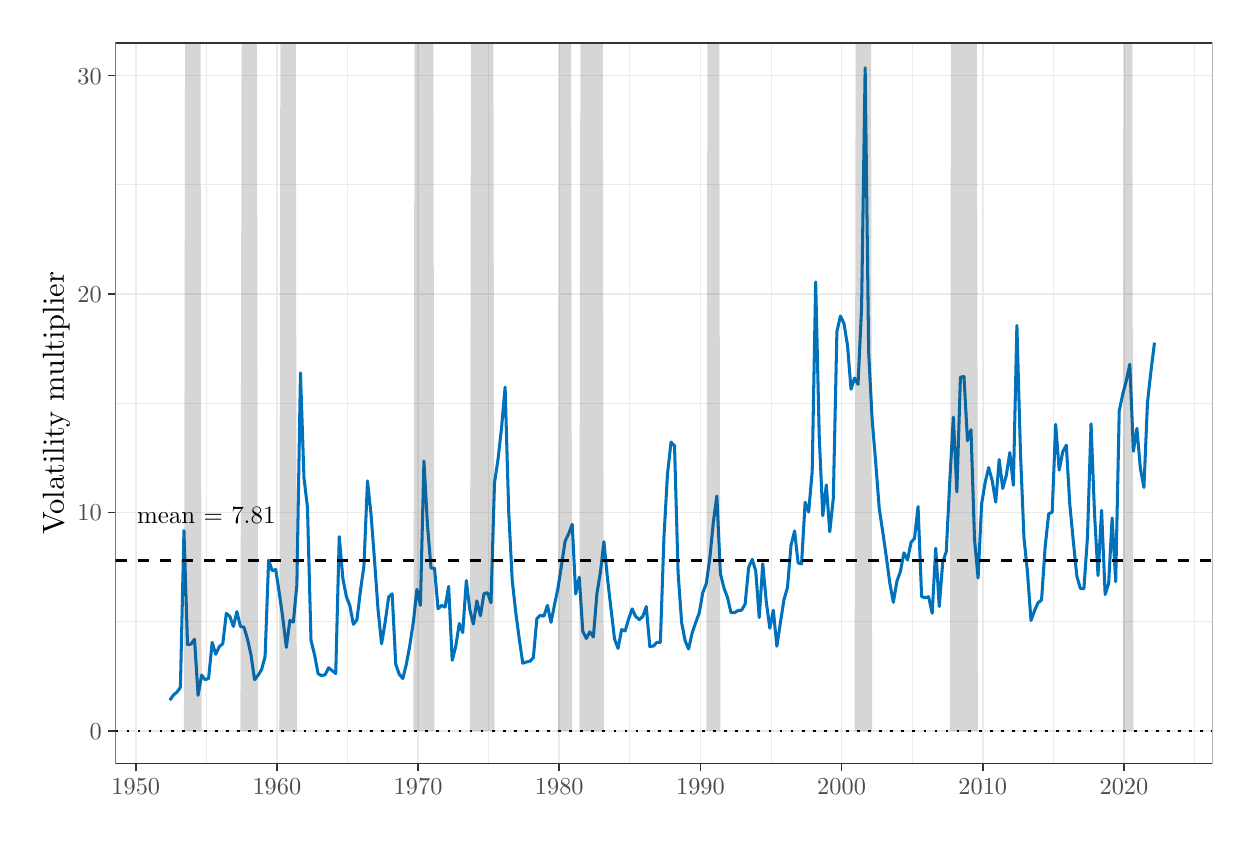
\begin{tikzpicture}[x=1pt,y=1pt]
\definecolor{fillColor}{RGB}{255,255,255}
\path[use as bounding box,fill=fillColor,fill opacity=0.00] (0,0) rectangle (433.62,289.08);
\begin{scope}
\path[clip] (  0.00,  0.00) rectangle (433.62,289.08);
\definecolor{drawColor}{RGB}{255,255,255}
\definecolor{fillColor}{RGB}{255,255,255}

\path[draw=drawColor,line width= 0.6pt,line join=round,line cap=round,fill=fillColor] (  0.00,  0.00) rectangle (433.62,289.08);
\end{scope}
\begin{scope}
\path[clip] ( 31.71, 23.11) rectangle (428.12,283.58);
\definecolor{fillColor}{RGB}{255,255,255}

\path[fill=fillColor] ( 31.71, 23.11) rectangle (428.12,283.58);
\definecolor{drawColor}{gray}{0.92}

\path[draw=drawColor,line width= 0.3pt,line join=round] ( 31.71, 74.41) --
	(428.12, 74.41);

\path[draw=drawColor,line width= 0.3pt,line join=round] ( 31.71,153.34) --
	(428.12,153.34);

\path[draw=drawColor,line width= 0.3pt,line join=round] ( 31.71,232.28) --
	(428.12,232.28);

\path[draw=drawColor,line width= 0.3pt,line join=round] ( 64.56, 23.11) --
	( 64.56,283.58);

\path[draw=drawColor,line width= 0.3pt,line join=round] (115.57, 23.11) --
	(115.57,283.58);

\path[draw=drawColor,line width= 0.3pt,line join=round] (166.59, 23.11) --
	(166.59,283.58);

\path[draw=drawColor,line width= 0.3pt,line join=round] (217.60, 23.11) --
	(217.60,283.58);

\path[draw=drawColor,line width= 0.3pt,line join=round] (268.61, 23.11) --
	(268.61,283.58);

\path[draw=drawColor,line width= 0.3pt,line join=round] (319.62, 23.11) --
	(319.62,283.58);

\path[draw=drawColor,line width= 0.3pt,line join=round] (370.64, 23.11) --
	(370.64,283.58);

\path[draw=drawColor,line width= 0.3pt,line join=round] (421.64, 23.11) --
	(421.64,283.58);

\path[draw=drawColor,line width= 0.6pt,line join=round] ( 31.71, 34.95) --
	(428.12, 34.95);

\path[draw=drawColor,line width= 0.6pt,line join=round] ( 31.71,113.88) --
	(428.12,113.88);

\path[draw=drawColor,line width= 0.6pt,line join=round] ( 31.71,192.81) --
	(428.12,192.81);

\path[draw=drawColor,line width= 0.6pt,line join=round] ( 31.71,271.74) --
	(428.12,271.74);

\path[draw=drawColor,line width= 0.6pt,line join=round] ( 39.06, 23.11) --
	( 39.06,283.58);

\path[draw=drawColor,line width= 0.6pt,line join=round] ( 90.06, 23.11) --
	( 90.06,283.58);

\path[draw=drawColor,line width= 0.6pt,line join=round] (141.08, 23.11) --
	(141.08,283.58);

\path[draw=drawColor,line width= 0.6pt,line join=round] (192.09, 23.11) --
	(192.09,283.58);

\path[draw=drawColor,line width= 0.6pt,line join=round] (243.11, 23.11) --
	(243.11,283.58);

\path[draw=drawColor,line width= 0.6pt,line join=round] (294.11, 23.11) --
	(294.11,283.58);

\path[draw=drawColor,line width= 0.6pt,line join=round] (345.13, 23.11) --
	(345.13,283.58);

\path[draw=drawColor,line width= 0.6pt,line join=round] (396.14, 23.11) --
	(396.14,283.58);
\definecolor{drawColor}{RGB}{0,114,189}

\path[draw=drawColor,line width= 1.1pt,line join=round] ( 51.38, 46.04) --
	( 52.66, 47.92) --
	( 53.93, 48.94) --
	( 55.19, 50.73) --
	( 56.47,107.36) --
	( 57.76, 66.17) --
	( 59.03, 66.34) --
	( 60.29, 68.09) --
	( 61.57, 47.82) --
	( 62.86, 55.13) --
	( 64.13, 53.47) --
	( 65.38, 53.96) --
	( 66.67, 66.96) --
	( 67.95, 62.65) --
	( 69.22, 65.38) --
	( 70.50, 66.45) --
	( 71.78, 77.44) --
	( 73.07, 76.31) --
	( 74.34, 72.68) --
	( 75.59, 78.09) --
	( 76.88, 72.69) --
	( 78.16, 72.45) --
	( 79.43, 68.14) --
	( 80.69, 62.51) --
	( 81.98, 53.49) --
	( 83.26, 55.04) --
	( 84.53, 57.15) --
	( 85.79, 61.88) --
	( 87.07, 96.65) --
	( 88.36, 92.86) --
	( 89.63, 93.25) --
	( 90.90, 84.90) --
	( 92.19, 75.80) --
	( 93.47, 65.15) --
	( 94.74, 74.90) --
	( 96.00, 74.28) --
	( 97.28, 87.82) --
	( 98.57,164.32) --
	( 99.84,126.39) --
	(101.10,115.80) --
	(102.38, 67.66) --
	(103.67, 62.44) --
	(104.94, 55.65) --
	(106.19, 54.93) --
	(107.48, 55.25) --
	(108.76, 57.79) --
	(110.03, 56.74) --
	(111.31, 55.69) --
	(112.59,105.19) --
	(113.88, 90.17) --
	(115.15, 83.51) --
	(116.40, 80.30) --
	(117.69, 73.48) --
	(118.97, 75.10) --
	(120.24, 85.61) --
	(121.50, 94.53) --
	(122.79,125.28) --
	(124.07,113.29) --
	(125.34, 96.52) --
	(126.60, 78.82) --
	(127.88, 66.42) --
	(129.17, 74.21) --
	(130.44, 83.33) --
	(131.71, 84.53) --
	(133.00, 59.04) --
	(134.28, 55.40) --
	(135.55, 53.88) --
	(136.81, 59.00) --
	(138.09, 65.88) --
	(139.38, 74.47) --
	(140.65, 86.13) --
	(141.91, 80.35) --
	(143.19,132.47) --
	(144.48,109.11) --
	(145.75, 93.79) --
	(147.00, 93.81) --
	(148.29, 79.11) --
	(149.57, 80.33) --
	(150.84, 79.69) --
	(152.12, 87.19) --
	(153.40, 60.48) --
	(154.69, 65.54) --
	(155.96, 73.79) --
	(157.21, 70.50) --
	(158.50, 89.30) --
	(159.78, 78.62) --
	(161.05, 73.57) --
	(162.31, 81.95) --
	(163.60, 76.57) --
	(164.88, 84.54) --
	(166.15, 84.92) --
	(167.41, 81.25) --
	(168.69,124.67) --
	(169.98,133.24) --
	(171.25,144.72) --
	(172.52,159.20) --
	(173.81,114.41) --
	(175.09, 89.36) --
	(176.36, 77.86) --
	(177.62, 68.31) --
	(178.90, 59.44) --
	(180.19, 59.86) --
	(181.46, 60.11) --
	(182.72, 61.41) --
	(184.00, 75.59) --
	(185.29, 76.77) --
	(186.56, 76.43) --
	(187.81, 80.34) --
	(189.10, 74.19) --
	(190.38, 80.62) --
	(191.65, 86.70) --
	(192.93, 95.02) --
	(194.21,103.55) --
	(195.50,106.24) --
	(196.77,109.62) --
	(198.02, 84.44) --
	(199.31, 90.53) --
	(200.59, 70.97) --
	(201.86, 68.37) --
	(203.12, 70.77) --
	(204.41, 68.90) --
	(205.69, 84.51) --
	(206.96, 92.28) --
	(208.22,103.34) --
	(209.50, 90.26) --
	(210.79, 79.02) --
	(212.06, 68.19) --
	(213.33, 64.78) --
	(214.62, 71.59) --
	(215.90, 71.11) --
	(217.17, 75.45) --
	(218.43, 79.06) --
	(219.71, 76.33) --
	(221.00, 75.14) --
	(222.27, 76.35) --
	(223.53, 79.89) --
	(224.81, 65.43) --
	(226.10, 65.65) --
	(227.37, 66.94) --
	(228.62, 66.92) --
	(229.91,104.88) --
	(231.19,127.79) --
	(232.47,139.32) --
	(233.74,137.96) --
	(235.02, 92.13) --
	(236.31, 74.07) --
	(237.58, 67.51) --
	(238.83, 64.58) --
	(240.12, 70.42) --
	(241.40, 74.14) --
	(242.67, 77.61) --
	(243.93, 84.85) --
	(245.22, 88.23) --
	(246.50, 97.43) --
	(247.77,110.46) --
	(249.03,119.86) --
	(250.31, 91.89) --
	(251.60, 86.58) --
	(252.87, 83.20) --
	(254.14, 77.70) --
	(255.43, 77.71) --
	(256.71, 78.46) --
	(257.98, 78.60) --
	(259.24, 80.78) --
	(260.52, 94.01) --
	(261.81, 96.94) --
	(263.08, 92.79) --
	(264.34, 75.94) --
	(265.62, 95.34) --
	(266.91, 81.41) --
	(268.18, 72.06) --
	(269.43, 78.57) --
	(270.72, 65.55) --
	(272.00, 74.10) --
	(273.28, 82.34) --
	(274.55, 86.82) --
	(275.83,102.05) --
	(277.12,107.22) --
	(278.39, 95.68) --
	(279.64, 95.33) --
	(280.93,117.59) --
	(282.21,114.06) --
	(283.48,128.77) --
	(284.74,197.19) --
	(286.03,141.29) --
	(287.31,112.71) --
	(288.58,123.87) --
	(289.84,106.92) --
	(291.12,119.08) --
	(292.41,179.23) --
	(293.68,184.88) --
	(294.95,182.22) --
	(296.24,174.31) --
	(297.52,158.42) --
	(298.79,162.48) --
	(300.05,160.19) --
	(301.33,187.92) --
	(302.62,274.60) --
	(303.89,171.71) --
	(305.15,147.57) --
	(306.43,131.95) --
	(307.72,115.27) --
	(308.99,106.81) --
	(310.24, 98.00) --
	(311.53, 88.40) --
	(312.81, 81.43) --
	(314.09, 89.07) --
	(315.36, 92.56) --
	(316.64, 99.33) --
	(317.93, 96.72) --
	(319.20,103.10) --
	(320.45,104.53) --
	(321.74,116.02) --
	(323.02, 83.51) --
	(324.29, 83.06) --
	(325.55, 83.43) --
	(326.84, 77.46) --
	(328.12,100.99) --
	(329.39, 79.90) --
	(330.65, 95.92) --
	(331.93, 99.75) --
	(333.22,125.71) --
	(334.49,148.38) --
	(335.76,121.34) --
	(337.05,162.78) --
	(338.33,163.01) --
	(339.60,139.83) --
	(340.86,143.81) --
	(342.14,104.14) --
	(343.43, 90.21) --
	(344.70,116.95) --
	(345.96,124.65) --
	(347.24,130.15) --
	(348.53,125.38) --
	(349.80,117.64) --
	(351.05,133.01) --
	(352.34,122.57) --
	(353.62,127.25) --
	(354.90,135.57) --
	(356.17,123.71) --
	(357.45,181.47) --
	(358.74,135.49) --
	(360.01,104.75) --
	(361.26, 92.42) --
	(362.55, 74.86) --
	(363.83, 78.44) --
	(365.10, 81.29) --
	(366.36, 82.26) --
	(367.65,101.35) --
	(368.93,113.41) --
	(370.20,113.98) --
	(371.46,145.74) --
	(372.74,129.18) --
	(374.03,135.87) --
	(375.30,138.21) --
	(376.57,116.84) --
	(377.86,103.29) --
	(379.14, 90.72) --
	(380.41, 86.41) --
	(381.67, 86.35) --
	(382.95,104.94) --
	(384.24,145.94) --
	(385.51,113.26) --
	(386.77, 91.11) --
	(388.05,114.68) --
	(389.34, 84.25) --
	(390.61, 88.31) --
	(391.86,111.92) --
	(393.15, 88.88) --
	(394.43,150.61) --
	(395.71,156.70) --
	(396.98,161.47) --
	(398.26,167.46) --
	(399.55,136.03) --
	(400.82,144.31) --
	(402.07,129.83) --
	(403.36,122.94) --
	(404.64,153.67) --
	(405.91,165.12) --
	(407.17,175.26);
\definecolor{fillColor}{RGB}{51,51,51}

\path[fill=fillColor,fill opacity=0.20] ( 50.09, 34.95) --
	( 50.45, 34.95) --
	( 51.02, 34.95) --
	( 51.38, 34.95) --
	( 51.73, 34.95) --
	( 52.30, 34.95) --
	( 52.66, 34.95) --
	( 53.02, 34.95) --
	( 53.57, 34.95) --
	( 53.93, 34.95) --
	( 54.29, 34.95) --
	( 54.83, 34.95) --
	( 55.19, 34.95) --
	( 55.55, 34.95) --
	( 56.11, 34.95) --
	( 56.47, 34.95) --
	( 56.83,255.88) --
	( 57.40,603.33) --
	( 57.76,824.25) --
	( 58.12,824.25) --
	( 58.67,824.25) --
	( 59.03,824.25) --
	( 59.39,824.25) --
	( 59.93,824.25) --
	( 60.29,824.25) --
	( 60.65,824.25) --
	( 61.21,824.25) --
	( 61.57,824.25) --
	( 61.93,603.33) --
	( 62.50,255.88) --
	( 62.86, 34.95) --
	( 63.22, 34.95) --
	( 63.77, 34.95) --
	( 64.13, 34.95) --
	( 64.49, 34.95) --
	( 65.02, 34.95) --
	( 65.38, 34.95) --
	( 65.74, 34.95) --
	( 66.31, 34.95) --
	( 66.67, 34.95) --
	( 67.03, 34.95) --
	( 67.59, 34.95) --
	( 67.95, 34.95) --
	( 68.31, 34.95) --
	( 68.86, 34.95) --
	( 69.22, 34.95) --
	( 69.58, 34.95) --
	( 70.14, 34.95) --
	( 70.50, 34.95) --
	( 70.86, 34.95) --
	( 71.42, 34.95) --
	( 71.78, 34.95) --
	( 72.14, 34.95) --
	( 72.71, 34.95) --
	( 73.07, 34.95) --
	( 73.42, 34.95) --
	( 73.98, 34.95) --
	( 74.34, 34.95) --
	( 74.70, 34.95) --
	( 75.23, 34.95) --
	( 75.59, 34.95) --
	( 75.95, 34.95) --
	( 76.52, 34.95) --
	( 76.88, 34.95) --
	( 77.24,255.88) --
	( 77.80,603.33) --
	( 78.16,824.25) --
	( 78.52,824.25) --
	( 79.07,824.25) --
	( 79.43,824.25) --
	( 79.79,824.25) --
	( 80.33,824.25) --
	( 80.69,824.25) --
	( 81.05,824.25) --
	( 81.62,824.25) --
	( 81.98,824.25) --
	( 82.34,603.33) --
	( 82.90,255.88) --
	( 83.26, 34.95) --
	( 83.62, 34.95) --
	( 84.17, 34.95) --
	( 84.53, 34.95) --
	( 84.89, 34.95) --
	( 85.43, 34.95) --
	( 85.79, 34.95) --
	( 86.15, 34.95) --
	( 86.71, 34.95) --
	( 87.07, 34.95) --
	( 87.43, 34.95) --
	( 88.00, 34.95) --
	( 88.36, 34.95) --
	( 88.72, 34.95) --
	( 89.27, 34.95) --
	( 89.63, 34.95) --
	( 89.99, 34.95) --
	( 90.54, 34.95) --
	( 90.90, 34.95) --
	( 91.26,255.88) --
	( 91.83,603.33) --
	( 92.19,824.25) --
	( 92.55,824.25) --
	( 93.11,824.25) --
	( 93.47,824.25) --
	( 93.83,824.25) --
	( 94.38,824.25) --
	( 94.74,824.25) --
	( 95.10,824.25) --
	( 95.64,824.25) --
	( 96.00,824.25) --
	( 96.36,603.33) --
	( 96.92,255.88) --
	( 97.28, 34.95) --
	( 97.64, 34.95) --
	( 98.21, 34.95) --
	( 98.57, 34.95) --
	( 98.93, 34.95) --
	( 99.48, 34.95) --
	( 99.84, 34.95) --
	(100.20, 34.95) --
	(100.74, 34.95) --
	(101.10, 34.95) --
	(101.46, 34.95) --
	(102.02, 34.95) --
	(102.38, 34.95) --
	(102.74, 34.95) --
	(103.31, 34.95) --
	(103.67, 34.95) --
	(104.03, 34.95) --
	(104.58, 34.95) --
	(104.94, 34.95) --
	(105.30, 34.95) --
	(105.83, 34.95) --
	(106.19, 34.95) --
	(106.55, 34.95) --
	(107.12, 34.95) --
	(107.48, 34.95) --
	(107.84, 34.95) --
	(108.40, 34.95) --
	(108.76, 34.95) --
	(109.12, 34.95) --
	(109.67, 34.95) --
	(110.03, 34.95) --
	(110.39, 34.95) --
	(110.95, 34.95) --
	(111.31, 34.95) --
	(111.67, 34.95) --
	(112.23, 34.95) --
	(112.59, 34.95) --
	(112.95, 34.95) --
	(113.52, 34.95) --
	(113.88, 34.95) --
	(114.24, 34.95) --
	(114.79, 34.95) --
	(115.15, 34.95) --
	(115.51, 34.95) --
	(116.04, 34.95) --
	(116.40, 34.95) --
	(116.76, 34.95) --
	(117.33, 34.95) --
	(117.69, 34.95) --
	(118.05, 34.95) --
	(118.61, 34.95) --
	(118.97, 34.95) --
	(119.33, 34.95) --
	(119.88, 34.95) --
	(120.24, 34.95) --
	(120.60, 34.95) --
	(121.14, 34.95) --
	(121.50, 34.95) --
	(121.86, 34.95) --
	(122.43, 34.95) --
	(122.79, 34.95) --
	(123.15, 34.95) --
	(123.71, 34.95) --
	(124.07, 34.95) --
	(124.43, 34.95) --
	(124.98, 34.95) --
	(125.34, 34.95) --
	(125.70, 34.95) --
	(126.24, 34.95) --
	(126.60, 34.95) --
	(126.96, 34.95) --
	(127.52, 34.95) --
	(127.88, 34.95) --
	(128.24, 34.95) --
	(128.81, 34.95) --
	(129.17, 34.95) --
	(129.53, 34.95) --
	(130.08, 34.95) --
	(130.44, 34.95) --
	(130.80, 34.95) --
	(131.35, 34.95) --
	(131.71, 34.95) --
	(132.07, 34.95) --
	(132.64, 34.95) --
	(133.00, 34.95) --
	(133.36, 34.95) --
	(133.92, 34.95) --
	(134.28, 34.95) --
	(134.64, 34.95) --
	(135.19, 34.95) --
	(135.55, 34.95) --
	(135.91, 34.95) --
	(136.45, 34.95) --
	(136.81, 34.95) --
	(137.17, 34.95) --
	(137.73, 34.95) --
	(138.09, 34.95) --
	(138.45, 34.95) --
	(139.02, 34.95) --
	(139.38, 34.95) --
	(139.74,258.30) --
	(140.29,600.90) --
	(140.65,824.25) --
	(141.01,824.25) --
	(141.55,824.25) --
	(141.91,824.25) --
	(142.27,824.25) --
	(142.83,824.25) --
	(143.19,824.25) --
	(143.55,824.25) --
	(144.12,824.25) --
	(144.48,824.25) --
	(144.84,824.25) --
	(145.39,824.25) --
	(145.75,824.25) --
	(146.11,598.42) --
	(146.64,260.79) --
	(147.00, 34.95) --
	(147.36, 34.95) --
	(147.93, 34.95) --
	(148.29, 34.95) --
	(148.65, 34.95) --
	(149.21, 34.95) --
	(149.57, 34.95) --
	(149.93, 34.95) --
	(150.49, 34.95) --
	(150.84, 34.95) --
	(151.20, 34.95) --
	(151.76, 34.95) --
	(152.12, 34.95) --
	(152.48, 34.95) --
	(153.04, 34.95) --
	(153.40, 34.95) --
	(153.76, 34.95) --
	(154.33, 34.95) --
	(154.69, 34.95) --
	(155.05, 34.95) --
	(155.60, 34.95) --
	(155.96, 34.95) --
	(156.32, 34.95) --
	(156.85, 34.95) --
	(157.21, 34.95) --
	(157.57, 34.95) --
	(158.14, 34.95) --
	(158.50, 34.95) --
	(158.86, 34.95) --
	(159.42, 34.95) --
	(159.78, 34.95) --
	(160.14,258.30) --
	(160.69,600.90) --
	(161.05,824.25) --
	(161.41,824.25) --
	(161.95,824.25) --
	(162.31,824.25) --
	(162.67,824.25) --
	(163.24,824.25) --
	(163.60,824.25) --
	(163.96,824.25) --
	(164.52,824.25) --
	(164.88,824.25) --
	(165.24,824.25) --
	(165.79,824.25) --
	(166.15,824.25) --
	(166.51,824.25) --
	(167.05,824.25) --
	(167.41,824.25) --
	(167.77,603.33) --
	(168.33,255.88) --
	(168.69, 34.95) --
	(169.05, 34.95) --
	(169.62, 34.95) --
	(169.98, 34.95) --
	(170.34, 34.95) --
	(170.89, 34.95) --
	(171.25, 34.95) --
	(171.61, 34.95) --
	(172.16, 34.95) --
	(172.52, 34.95) --
	(172.88, 34.95) --
	(173.45, 34.95) --
	(173.81, 34.95) --
	(174.17, 34.95) --
	(174.73, 34.95) --
	(175.09, 34.95) --
	(175.45, 34.95) --
	(176.00, 34.95) --
	(176.36, 34.95) --
	(176.72, 34.95) --
	(177.26, 34.95) --
	(177.62, 34.95) --
	(177.98, 34.95) --
	(178.54, 34.95) --
	(178.90, 34.95) --
	(179.26, 34.95) --
	(179.83, 34.95) --
	(180.19, 34.95) --
	(180.55, 34.95) --
	(181.10, 34.95) --
	(181.46, 34.95) --
	(181.82, 34.95) --
	(182.36, 34.95) --
	(182.72, 34.95) --
	(183.08, 34.95) --
	(183.64, 34.95) --
	(184.00, 34.95) --
	(184.36, 34.95) --
	(184.93, 34.95) --
	(185.29, 34.95) --
	(185.65, 34.95) --
	(186.20, 34.95) --
	(186.56, 34.95) --
	(186.92, 34.95) --
	(187.45, 34.95) --
	(187.81, 34.95) --
	(188.17, 34.95) --
	(188.74, 34.95) --
	(189.10, 34.95) --
	(189.46, 34.95) --
	(190.02, 34.95) --
	(190.38, 34.95) --
	(190.74, 34.95) --
	(191.30, 34.95) --
	(191.65, 34.95) --
	(192.01,258.30) --
	(192.57,600.90) --
	(192.93,824.25) --
	(193.29,824.25) --
	(193.85,824.25) --
	(194.21,824.25) --
	(194.57,824.25) --
	(195.14,824.25) --
	(195.50,824.25) --
	(195.86,600.90) --
	(196.41,258.30) --
	(196.77, 34.95) --
	(197.13, 34.95) --
	(197.66, 34.95) --
	(198.02, 34.95) --
	(198.38, 34.95) --
	(198.95, 34.95) --
	(199.31, 34.95) --
	(199.67,255.88) --
	(200.23,603.33) --
	(200.59,824.25) --
	(200.95,824.25) --
	(201.50,824.25) --
	(201.86,824.25) --
	(202.22,824.25) --
	(202.76,824.25) --
	(203.12,824.25) --
	(203.48,824.25) --
	(204.05,824.25) --
	(204.41,824.25) --
	(204.77,824.25) --
	(205.33,824.25) --
	(205.69,824.25) --
	(206.05,824.25) --
	(206.60,824.25) --
	(206.96,824.25) --
	(207.32,598.42) --
	(207.86,260.79) --
	(208.22, 34.95) --
	(208.58, 34.95) --
	(209.14, 34.95) --
	(209.50, 34.95) --
	(209.86, 34.95) --
	(210.43, 34.95) --
	(210.79, 34.95) --
	(211.15, 34.95) --
	(211.70, 34.95) --
	(212.06, 34.95) --
	(212.42, 34.95) --
	(212.97, 34.95) --
	(213.33, 34.95) --
	(213.69, 34.95) --
	(214.26, 34.95) --
	(214.62, 34.95) --
	(214.98, 34.95) --
	(215.54, 34.95) --
	(215.90, 34.95) --
	(216.26, 34.95) --
	(216.81, 34.95) --
	(217.17, 34.95) --
	(217.53, 34.95) --
	(218.07, 34.95) --
	(218.43, 34.95) --
	(218.79, 34.95) --
	(219.35, 34.95) --
	(219.71, 34.95) --
	(220.07, 34.95) --
	(220.64, 34.95) --
	(221.00, 34.95) --
	(221.36, 34.95) --
	(221.91, 34.95) --
	(222.27, 34.95) --
	(222.63, 34.95) --
	(223.17, 34.95) --
	(223.53, 34.95) --
	(223.89, 34.95) --
	(224.45, 34.95) --
	(224.81, 34.95) --
	(225.17, 34.95) --
	(225.74, 34.95) --
	(226.10, 34.95) --
	(226.46, 34.95) --
	(227.01, 34.95) --
	(227.37, 34.95) --
	(227.73, 34.95) --
	(228.26, 34.95) --
	(228.62, 34.95) --
	(228.98, 34.95) --
	(229.55, 34.95) --
	(229.91, 34.95) --
	(230.27, 34.95) --
	(230.83, 34.95) --
	(231.19, 34.95) --
	(231.55, 34.95) --
	(232.11, 34.95) --
	(232.47, 34.95) --
	(232.82, 34.95) --
	(233.38, 34.95) --
	(233.74, 34.95) --
	(234.10, 34.95) --
	(234.66, 34.95) --
	(235.02, 34.95) --
	(235.38, 34.95) --
	(235.95, 34.95) --
	(236.31, 34.95) --
	(236.67, 34.95) --
	(237.22, 34.95) --
	(237.58, 34.95) --
	(237.94, 34.95) --
	(238.47, 34.95) --
	(238.83, 34.95) --
	(239.19, 34.95) --
	(239.76, 34.95) --
	(240.12, 34.95) --
	(240.48, 34.95) --
	(241.04, 34.95) --
	(241.40, 34.95) --
	(241.76, 34.95) --
	(242.31, 34.95) --
	(242.67, 34.95) --
	(243.03, 34.95) --
	(243.57, 34.95) --
	(243.93, 34.95) --
	(244.29, 34.95) --
	(244.86, 34.95) --
	(245.22, 34.95) --
	(245.58,255.88) --
	(246.14,603.33) --
	(246.50,824.25) --
	(246.86,824.25) --
	(247.41,824.25) --
	(247.77,824.25) --
	(248.13,824.25) --
	(248.67,824.25) --
	(249.03,824.25) --
	(249.39,603.33) --
	(249.95,255.88) --
	(250.31, 34.95) --
	(250.67, 34.95) --
	(251.24, 34.95) --
	(251.60, 34.95) --
	(251.96, 34.95) --
	(252.51, 34.95) --
	(252.87, 34.95) --
	(253.23, 34.95) --
	(253.78, 34.95) --
	(254.14, 34.95) --
	(254.50, 34.95) --
	(255.07, 34.95) --
	(255.43, 34.95) --
	(255.79, 34.95) --
	(256.35, 34.95) --
	(256.71, 34.95) --
	(257.07, 34.95) --
	(257.62, 34.95) --
	(257.98, 34.95) --
	(258.34, 34.95) --
	(258.88, 34.95) --
	(259.24, 34.95) --
	(259.60, 34.95) --
	(260.16, 34.95) --
	(260.52, 34.95) --
	(260.88, 34.95) --
	(261.45, 34.95) --
	(261.81, 34.95) --
	(262.17, 34.95) --
	(262.72, 34.95) --
	(263.08, 34.95) --
	(263.44, 34.95) --
	(263.98, 34.95) --
	(264.34, 34.95) --
	(264.70, 34.95) --
	(265.26, 34.95) --
	(265.62, 34.95) --
	(265.98, 34.95) --
	(266.55, 34.95) --
	(266.91, 34.95) --
	(267.27, 34.95) --
	(267.82, 34.95) --
	(268.18, 34.95) --
	(268.54, 34.95) --
	(269.07, 34.95) --
	(269.43, 34.95) --
	(269.79, 34.95) --
	(270.36, 34.95) --
	(270.72, 34.95) --
	(271.08, 34.95) --
	(271.64, 34.95) --
	(272.00, 34.95) --
	(272.36, 34.95) --
	(272.92, 34.95) --
	(273.28, 34.95) --
	(273.63, 34.95) --
	(274.19, 34.95) --
	(274.55, 34.95) --
	(274.91, 34.95) --
	(275.47, 34.95) --
	(275.83, 34.95) --
	(276.19, 34.95) --
	(276.76, 34.95) --
	(277.12, 34.95) --
	(277.48, 34.95) --
	(278.03, 34.95) --
	(278.39, 34.95) --
	(278.75, 34.95) --
	(279.28, 34.95) --
	(279.64, 34.95) --
	(280.00, 34.95) --
	(280.57, 34.95) --
	(280.93, 34.95) --
	(281.29, 34.95) --
	(281.85, 34.95) --
	(282.21, 34.95) --
	(282.57, 34.95) --
	(283.12, 34.95) --
	(283.48, 34.95) --
	(283.84, 34.95) --
	(284.38, 34.95) --
	(284.74, 34.95) --
	(285.10, 34.95) --
	(285.67, 34.95) --
	(286.03, 34.95) --
	(286.39, 34.95) --
	(286.95, 34.95) --
	(287.31, 34.95) --
	(287.67, 34.95) --
	(288.22, 34.95) --
	(288.58, 34.95) --
	(288.94, 34.95) --
	(289.48, 34.95) --
	(289.84, 34.95) --
	(290.20, 34.95) --
	(290.76, 34.95) --
	(291.12, 34.95) --
	(291.48, 34.95) --
	(292.05, 34.95) --
	(292.41, 34.95) --
	(292.77, 34.95) --
	(293.32, 34.95) --
	(293.68, 34.95) --
	(294.04, 34.95) --
	(294.59, 34.95) --
	(294.95, 34.95) --
	(295.31, 34.95) --
	(295.88, 34.95) --
	(296.24, 34.95) --
	(296.60, 34.95) --
	(297.16, 34.95) --
	(297.52, 34.95) --
	(297.88, 34.95) --
	(298.43, 34.95) --
	(298.79, 34.95) --
	(299.15,260.79) --
	(299.69,598.42) --
	(300.05,824.25) --
	(300.41,824.25) --
	(300.97,824.25) --
	(301.33,824.25) --
	(301.69,824.25) --
	(302.26,824.25) --
	(302.62,824.25) --
	(302.98,824.25) --
	(303.53,824.25) --
	(303.89,824.25) --
	(304.25,598.42) --
	(304.79,260.79) --
	(305.15, 34.95) --
	(305.51, 34.95) --
	(306.07, 34.95) --
	(306.43, 34.95) --
	(306.79, 34.95) --
	(307.36, 34.95) --
	(307.72, 34.95) --
	(308.08, 34.95) --
	(308.63, 34.95) --
	(308.99, 34.95) --
	(309.35, 34.95) --
	(309.88, 34.95) --
	(310.24, 34.95) --
	(310.60, 34.95) --
	(311.17, 34.95) --
	(311.53, 34.95) --
	(311.89, 34.95) --
	(312.45, 34.95) --
	(312.81, 34.95) --
	(313.17, 34.95) --
	(313.73, 34.95) --
	(314.09, 34.95) --
	(314.44, 34.95) --
	(315.00, 34.95) --
	(315.36, 34.95) --
	(315.72, 34.95) --
	(316.28, 34.95) --
	(316.64, 34.95) --
	(317.00, 34.95) --
	(317.57, 34.95) --
	(317.93, 34.95) --
	(318.29, 34.95) --
	(318.84, 34.95) --
	(319.20, 34.95) --
	(319.56, 34.95) --
	(320.09, 34.95) --
	(320.45, 34.95) --
	(320.81, 34.95) --
	(321.38, 34.95) --
	(321.74, 34.95) --
	(322.10, 34.95) --
	(322.66, 34.95) --
	(323.02, 34.95) --
	(323.38, 34.95) --
	(323.94, 34.95) --
	(324.29, 34.95) --
	(324.65, 34.95) --
	(325.19, 34.95) --
	(325.55, 34.95) --
	(325.91, 34.95) --
	(326.48, 34.95) --
	(326.84, 34.95) --
	(327.20, 34.95) --
	(327.76, 34.95) --
	(328.12, 34.95) --
	(328.48, 34.95) --
	(329.03, 34.95) --
	(329.39, 34.95) --
	(329.75, 34.95) --
	(330.29, 34.95) --
	(330.65, 34.95) --
	(331.01, 34.95) --
	(331.57, 34.95) --
	(331.93, 34.95) --
	(332.29, 34.95) --
	(332.86, 34.95) --
	(333.22, 34.95) --
	(333.58,258.30) --
	(334.13,600.90) --
	(334.49,824.25) --
	(334.85,824.25) --
	(335.40,824.25) --
	(335.76,824.25) --
	(336.12,824.25) --
	(336.69,824.25) --
	(337.05,824.25) --
	(337.41,824.25) --
	(337.97,824.25) --
	(338.33,824.25) --
	(338.69,824.25) --
	(339.24,824.25) --
	(339.60,824.25) --
	(339.96,824.25) --
	(340.50,824.25) --
	(340.86,824.25) --
	(341.22,824.25) --
	(341.78,824.25) --
	(342.14,824.25) --
	(342.50,603.33) --
	(343.07,255.88) --
	(343.43, 34.95) --
	(343.79, 34.95) --
	(344.34, 34.95) --
	(344.70, 34.95) --
	(345.06, 34.95) --
	(345.60, 34.95) --
	(345.96, 34.95) --
	(346.32, 34.95) --
	(346.88, 34.95) --
	(347.24, 34.95) --
	(347.60, 34.95) --
	(348.17, 34.95) --
	(348.53, 34.95) --
	(348.89, 34.95) --
	(349.44, 34.95) --
	(349.80, 34.95) --
	(350.16, 34.95) --
	(350.69, 34.95) --
	(351.05, 34.95) --
	(351.41, 34.95) --
	(351.98, 34.95) --
	(352.34, 34.95) --
	(352.70, 34.95) --
	(353.26, 34.95) --
	(353.62, 34.95) --
	(353.98, 34.95) --
	(354.54, 34.95) --
	(354.90, 34.95) --
	(355.26, 34.95) --
	(355.81, 34.95) --
	(356.17, 34.95) --
	(356.53, 34.95) --
	(357.09, 34.95) --
	(357.45, 34.95) --
	(357.81, 34.95) --
	(358.38, 34.95) --
	(358.74, 34.95) --
	(359.10, 34.95) --
	(359.65, 34.95) --
	(360.01, 34.95) --
	(360.37, 34.95) --
	(360.90, 34.95) --
	(361.26, 34.95) --
	(361.62, 34.95) --
	(362.19, 34.95) --
	(362.55, 34.95) --
	(362.91, 34.95) --
	(363.47, 34.95) --
	(363.83, 34.95) --
	(364.19, 34.95) --
	(364.75, 34.95) --
	(365.10, 34.95) --
	(365.46, 34.95) --
	(366.00, 34.95) --
	(366.36, 34.95) --
	(366.72, 34.95) --
	(367.29, 34.95) --
	(367.65, 34.95) --
	(368.01, 34.95) --
	(368.57, 34.95) --
	(368.93, 34.95) --
	(369.29, 34.95) --
	(369.84, 34.95) --
	(370.20, 34.95) --
	(370.56, 34.95) --
	(371.10, 34.95) --
	(371.46, 34.95) --
	(371.82, 34.95) --
	(372.38, 34.95) --
	(372.74, 34.95) --
	(373.10, 34.95) --
	(373.67, 34.95) --
	(374.03, 34.95) --
	(374.39, 34.95) --
	(374.94, 34.95) --
	(375.30, 34.95) --
	(375.66, 34.95) --
	(376.21, 34.95) --
	(376.57, 34.95) --
	(376.93, 34.95) --
	(377.50, 34.95) --
	(377.86, 34.95) --
	(378.22, 34.95) --
	(378.78, 34.95) --
	(379.14, 34.95) --
	(379.50, 34.95) --
	(380.05, 34.95) --
	(380.41, 34.95) --
	(380.77, 34.95) --
	(381.31, 34.95) --
	(381.67, 34.95) --
	(382.03, 34.95) --
	(382.59, 34.95) --
	(382.95, 34.95) --
	(383.31, 34.95) --
	(383.88, 34.95) --
	(384.24, 34.95) --
	(384.60, 34.95) --
	(385.15, 34.95) --
	(385.51, 34.95) --
	(385.87, 34.95) --
	(386.41, 34.95) --
	(386.77, 34.95) --
	(387.13, 34.95) --
	(387.69, 34.95) --
	(388.05, 34.95) --
	(388.41, 34.95) --
	(388.98, 34.95) --
	(389.34, 34.95) --
	(389.70, 34.95) --
	(390.25, 34.95) --
	(390.61, 34.95) --
	(390.97, 34.95) --
	(391.51, 34.95) --
	(391.86, 34.95) --
	(392.22, 34.95) --
	(392.79, 34.95) --
	(393.15, 34.95) --
	(393.51, 34.95) --
	(394.07, 34.95) --
	(394.43, 34.95) --
	(394.79, 34.95) --
	(395.35, 34.95) --
	(395.71, 34.95) --
	(396.07,258.30) --
	(396.62,600.90) --
	(396.98,824.25) --
	(397.34,824.25) --
	(397.90,824.25) --
	(398.26,824.25) --
	(398.62,603.33) --
	(399.19,255.88) --
	(399.55, 34.95) --
	(399.91, 34.95) --
	(400.46, 34.95) --
	(400.82, 34.95) --
	(401.18, 34.95) --
	(401.71, 34.95) --
	(402.07, 34.95) --
	(402.43, 34.95) --
	(403.00, 34.95) --
	(403.36, 34.95) --
	(403.72, 34.95) --
	(404.28, 34.95) --
	(404.64, 34.95) --
	(405.00, 34.95) --
	(405.56, 34.95) --
	(405.91, 34.95) --
	(406.27, 34.95) --
	(406.81, 34.95) --
	(407.17, 34.95) --
	(407.53, 34.95) --
	(408.10, 34.95) --
	(408.46, 34.95) --
	(408.82, 34.95) --
	(409.38, 34.95) --
	(409.74, 34.95) --
	(410.10, 34.95) --
	(409.74, 34.95) --
	(409.38, 34.95) --
	(408.82, 34.95) --
	(408.46, 34.95) --
	(408.10, 34.95) --
	(407.53, 34.95) --
	(407.17, 34.95) --
	(406.81, 34.95) --
	(406.27, 34.95) --
	(405.91, 34.95) --
	(405.56, 34.95) --
	(405.00, 34.95) --
	(404.64, 34.95) --
	(404.28, 34.95) --
	(403.72, 34.95) --
	(403.36, 34.95) --
	(403.00, 34.95) --
	(402.43, 34.95) --
	(402.07, 34.95) --
	(401.71, 34.95) --
	(401.18, 34.95) --
	(400.82, 34.95) --
	(400.46, 34.95) --
	(399.91, 34.95) --
	(399.55, 34.95) --
	(399.19, 34.95) --
	(398.62, 34.95) --
	(398.26, 34.95) --
	(397.90, 34.95) --
	(397.34, 34.95) --
	(396.98, 34.95) --
	(396.62, 34.95) --
	(396.07, 34.95) --
	(395.71, 34.95) --
	(395.35, 34.95) --
	(394.79, 34.95) --
	(394.43, 34.95) --
	(394.07, 34.95) --
	(393.51, 34.95) --
	(393.15, 34.95) --
	(392.79, 34.95) --
	(392.22, 34.95) --
	(391.86, 34.95) --
	(391.51, 34.95) --
	(390.97, 34.95) --
	(390.61, 34.95) --
	(390.25, 34.95) --
	(389.70, 34.95) --
	(389.34, 34.95) --
	(388.98, 34.95) --
	(388.41, 34.95) --
	(388.05, 34.95) --
	(387.69, 34.95) --
	(387.13, 34.95) --
	(386.77, 34.95) --
	(386.41, 34.95) --
	(385.87, 34.95) --
	(385.51, 34.95) --
	(385.15, 34.95) --
	(384.60, 34.95) --
	(384.24, 34.95) --
	(383.88, 34.95) --
	(383.31, 34.95) --
	(382.95, 34.95) --
	(382.59, 34.95) --
	(382.03, 34.95) --
	(381.67, 34.95) --
	(381.31, 34.95) --
	(380.77, 34.95) --
	(380.41, 34.95) --
	(380.05, 34.95) --
	(379.50, 34.95) --
	(379.14, 34.95) --
	(378.78, 34.95) --
	(378.22, 34.95) --
	(377.86, 34.95) --
	(377.50, 34.95) --
	(376.93, 34.95) --
	(376.57, 34.95) --
	(376.21, 34.95) --
	(375.66, 34.95) --
	(375.30, 34.95) --
	(374.94, 34.95) --
	(374.39, 34.95) --
	(374.03, 34.95) --
	(373.67, 34.95) --
	(373.10, 34.95) --
	(372.74, 34.95) --
	(372.38, 34.95) --
	(371.82, 34.95) --
	(371.46, 34.95) --
	(371.10, 34.95) --
	(370.56, 34.95) --
	(370.20, 34.95) --
	(369.84, 34.95) --
	(369.29, 34.95) --
	(368.93, 34.95) --
	(368.57, 34.95) --
	(368.01, 34.95) --
	(367.65, 34.95) --
	(367.29, 34.95) --
	(366.72, 34.95) --
	(366.36, 34.95) --
	(366.00, 34.95) --
	(365.46, 34.95) --
	(365.10, 34.95) --
	(364.75, 34.95) --
	(364.19, 34.95) --
	(363.83, 34.95) --
	(363.47, 34.95) --
	(362.91, 34.95) --
	(362.55, 34.95) --
	(362.19, 34.95) --
	(361.62, 34.95) --
	(361.26, 34.95) --
	(360.90, 34.95) --
	(360.37, 34.95) --
	(360.01, 34.95) --
	(359.65, 34.95) --
	(359.10, 34.95) --
	(358.74, 34.95) --
	(358.38, 34.95) --
	(357.81, 34.95) --
	(357.45, 34.95) --
	(357.09, 34.95) --
	(356.53, 34.95) --
	(356.17, 34.95) --
	(355.81, 34.95) --
	(355.26, 34.95) --
	(354.90, 34.95) --
	(354.54, 34.95) --
	(353.98, 34.95) --
	(353.62, 34.95) --
	(353.26, 34.95) --
	(352.70, 34.95) --
	(352.34, 34.95) --
	(351.98, 34.95) --
	(351.41, 34.95) --
	(351.05, 34.95) --
	(350.69, 34.95) --
	(350.16, 34.95) --
	(349.80, 34.95) --
	(349.44, 34.95) --
	(348.89, 34.95) --
	(348.53, 34.95) --
	(348.17, 34.95) --
	(347.60, 34.95) --
	(347.24, 34.95) --
	(346.88, 34.95) --
	(346.32, 34.95) --
	(345.96, 34.95) --
	(345.60, 34.95) --
	(345.06, 34.95) --
	(344.70, 34.95) --
	(344.34, 34.95) --
	(343.79, 34.95) --
	(343.43, 34.95) --
	(343.07, 34.95) --
	(342.50, 34.95) --
	(342.14, 34.95) --
	(341.78, 34.95) --
	(341.22, 34.95) --
	(340.86, 34.95) --
	(340.50, 34.95) --
	(339.96, 34.95) --
	(339.60, 34.95) --
	(339.24, 34.95) --
	(338.69, 34.95) --
	(338.33, 34.95) --
	(337.97, 34.95) --
	(337.41, 34.95) --
	(337.05, 34.95) --
	(336.69, 34.95) --
	(336.12, 34.95) --
	(335.76, 34.95) --
	(335.40, 34.95) --
	(334.85, 34.95) --
	(334.49, 34.95) --
	(334.13, 34.95) --
	(333.58, 34.95) --
	(333.22, 34.95) --
	(332.86, 34.95) --
	(332.29, 34.95) --
	(331.93, 34.95) --
	(331.57, 34.95) --
	(331.01, 34.95) --
	(330.65, 34.95) --
	(330.29, 34.95) --
	(329.75, 34.95) --
	(329.39, 34.95) --
	(329.03, 34.95) --
	(328.48, 34.95) --
	(328.12, 34.95) --
	(327.76, 34.95) --
	(327.20, 34.95) --
	(326.84, 34.95) --
	(326.48, 34.95) --
	(325.91, 34.95) --
	(325.55, 34.95) --
	(325.19, 34.95) --
	(324.65, 34.95) --
	(324.29, 34.95) --
	(323.94, 34.95) --
	(323.38, 34.95) --
	(323.02, 34.95) --
	(322.66, 34.95) --
	(322.10, 34.95) --
	(321.74, 34.95) --
	(321.38, 34.95) --
	(320.81, 34.95) --
	(320.45, 34.95) --
	(320.09, 34.95) --
	(319.56, 34.95) --
	(319.20, 34.95) --
	(318.84, 34.95) --
	(318.29, 34.95) --
	(317.93, 34.95) --
	(317.57, 34.95) --
	(317.00, 34.95) --
	(316.64, 34.95) --
	(316.28, 34.95) --
	(315.72, 34.95) --
	(315.36, 34.95) --
	(315.00, 34.95) --
	(314.44, 34.95) --
	(314.09, 34.95) --
	(313.73, 34.95) --
	(313.17, 34.95) --
	(312.81, 34.95) --
	(312.45, 34.95) --
	(311.89, 34.95) --
	(311.53, 34.95) --
	(311.17, 34.95) --
	(310.60, 34.95) --
	(310.24, 34.95) --
	(309.88, 34.95) --
	(309.35, 34.95) --
	(308.99, 34.95) --
	(308.63, 34.95) --
	(308.08, 34.95) --
	(307.72, 34.95) --
	(307.36, 34.95) --
	(306.79, 34.95) --
	(306.43, 34.95) --
	(306.07, 34.95) --
	(305.51, 34.95) --
	(305.15, 34.95) --
	(304.79, 34.95) --
	(304.25, 34.95) --
	(303.89, 34.95) --
	(303.53, 34.95) --
	(302.98, 34.95) --
	(302.62, 34.95) --
	(302.26, 34.95) --
	(301.69, 34.95) --
	(301.33, 34.95) --
	(300.97, 34.95) --
	(300.41, 34.95) --
	(300.05, 34.95) --
	(299.69, 34.95) --
	(299.15, 34.95) --
	(298.79, 34.95) --
	(298.43, 34.95) --
	(297.88, 34.95) --
	(297.52, 34.95) --
	(297.16, 34.95) --
	(296.60, 34.95) --
	(296.24, 34.95) --
	(295.88, 34.95) --
	(295.31, 34.95) --
	(294.95, 34.95) --
	(294.59, 34.95) --
	(294.04, 34.95) --
	(293.68, 34.95) --
	(293.32, 34.95) --
	(292.77, 34.95) --
	(292.41, 34.95) --
	(292.05, 34.95) --
	(291.48, 34.95) --
	(291.12, 34.95) --
	(290.76, 34.95) --
	(290.20, 34.95) --
	(289.84, 34.95) --
	(289.48, 34.95) --
	(288.94, 34.95) --
	(288.58, 34.95) --
	(288.22, 34.95) --
	(287.67, 34.95) --
	(287.31, 34.95) --
	(286.95, 34.95) --
	(286.39, 34.95) --
	(286.03, 34.95) --
	(285.67, 34.95) --
	(285.10, 34.95) --
	(284.74, 34.95) --
	(284.38, 34.95) --
	(283.84, 34.95) --
	(283.48, 34.95) --
	(283.12, 34.95) --
	(282.57, 34.95) --
	(282.21, 34.95) --
	(281.85, 34.95) --
	(281.29, 34.95) --
	(280.93, 34.95) --
	(280.57, 34.95) --
	(280.00, 34.95) --
	(279.64, 34.95) --
	(279.28, 34.95) --
	(278.75, 34.95) --
	(278.39, 34.95) --
	(278.03, 34.95) --
	(277.48, 34.95) --
	(277.12, 34.95) --
	(276.76, 34.95) --
	(276.19, 34.95) --
	(275.83, 34.95) --
	(275.47, 34.95) --
	(274.91, 34.95) --
	(274.55, 34.95) --
	(274.19, 34.95) --
	(273.63, 34.95) --
	(273.28, 34.95) --
	(272.92, 34.95) --
	(272.36, 34.95) --
	(272.00, 34.95) --
	(271.64, 34.95) --
	(271.08, 34.95) --
	(270.72, 34.95) --
	(270.36, 34.95) --
	(269.79, 34.95) --
	(269.43, 34.95) --
	(269.07, 34.95) --
	(268.54, 34.95) --
	(268.18, 34.95) --
	(267.82, 34.95) --
	(267.27, 34.95) --
	(266.91, 34.95) --
	(266.55, 34.95) --
	(265.98, 34.95) --
	(265.62, 34.95) --
	(265.26, 34.95) --
	(264.70, 34.95) --
	(264.34, 34.95) --
	(263.98, 34.95) --
	(263.44, 34.95) --
	(263.08, 34.95) --
	(262.72, 34.95) --
	(262.17, 34.95) --
	(261.81, 34.95) --
	(261.45, 34.95) --
	(260.88, 34.95) --
	(260.52, 34.95) --
	(260.16, 34.95) --
	(259.60, 34.95) --
	(259.24, 34.95) --
	(258.88, 34.95) --
	(258.34, 34.95) --
	(257.98, 34.95) --
	(257.62, 34.95) --
	(257.07, 34.95) --
	(256.71, 34.95) --
	(256.35, 34.95) --
	(255.79, 34.95) --
	(255.43, 34.95) --
	(255.07, 34.95) --
	(254.50, 34.95) --
	(254.14, 34.95) --
	(253.78, 34.95) --
	(253.23, 34.95) --
	(252.87, 34.95) --
	(252.51, 34.95) --
	(251.96, 34.95) --
	(251.60, 34.95) --
	(251.24, 34.95) --
	(250.67, 34.95) --
	(250.31, 34.95) --
	(249.95, 34.95) --
	(249.39, 34.95) --
	(249.03, 34.95) --
	(248.67, 34.95) --
	(248.13, 34.95) --
	(247.77, 34.95) --
	(247.41, 34.95) --
	(246.86, 34.95) --
	(246.50, 34.95) --
	(246.14, 34.95) --
	(245.58, 34.95) --
	(245.22, 34.95) --
	(244.86, 34.95) --
	(244.29, 34.95) --
	(243.93, 34.95) --
	(243.57, 34.95) --
	(243.03, 34.95) --
	(242.67, 34.95) --
	(242.31, 34.95) --
	(241.76, 34.95) --
	(241.40, 34.95) --
	(241.04, 34.95) --
	(240.48, 34.95) --
	(240.12, 34.95) --
	(239.76, 34.95) --
	(239.19, 34.95) --
	(238.83, 34.95) --
	(238.47, 34.95) --
	(237.94, 34.95) --
	(237.58, 34.95) --
	(237.22, 34.95) --
	(236.67, 34.95) --
	(236.31, 34.95) --
	(235.95, 34.95) --
	(235.38, 34.95) --
	(235.02, 34.95) --
	(234.66, 34.95) --
	(234.10, 34.95) --
	(233.74, 34.95) --
	(233.38, 34.95) --
	(232.82, 34.95) --
	(232.47, 34.95) --
	(232.11, 34.95) --
	(231.55, 34.95) --
	(231.19, 34.95) --
	(230.83, 34.95) --
	(230.27, 34.95) --
	(229.91, 34.95) --
	(229.55, 34.95) --
	(228.98, 34.95) --
	(228.62, 34.95) --
	(228.26, 34.95) --
	(227.73, 34.95) --
	(227.37, 34.95) --
	(227.01, 34.95) --
	(226.46, 34.95) --
	(226.10, 34.95) --
	(225.74, 34.95) --
	(225.17, 34.95) --
	(224.81, 34.95) --
	(224.45, 34.95) --
	(223.89, 34.95) --
	(223.53, 34.95) --
	(223.17, 34.95) --
	(222.63, 34.95) --
	(222.27, 34.95) --
	(221.91, 34.95) --
	(221.36, 34.95) --
	(221.00, 34.95) --
	(220.64, 34.95) --
	(220.07, 34.95) --
	(219.71, 34.95) --
	(219.35, 34.95) --
	(218.79, 34.95) --
	(218.43, 34.95) --
	(218.07, 34.95) --
	(217.53, 34.95) --
	(217.17, 34.95) --
	(216.81, 34.95) --
	(216.26, 34.95) --
	(215.90, 34.95) --
	(215.54, 34.95) --
	(214.98, 34.95) --
	(214.62, 34.95) --
	(214.26, 34.95) --
	(213.69, 34.95) --
	(213.33, 34.95) --
	(212.97, 34.95) --
	(212.42, 34.95) --
	(212.06, 34.95) --
	(211.70, 34.95) --
	(211.15, 34.95) --
	(210.79, 34.95) --
	(210.43, 34.95) --
	(209.86, 34.95) --
	(209.50, 34.95) --
	(209.14, 34.95) --
	(208.58, 34.95) --
	(208.22, 34.95) --
	(207.86, 34.95) --
	(207.32, 34.95) --
	(206.96, 34.95) --
	(206.60, 34.95) --
	(206.05, 34.95) --
	(205.69, 34.95) --
	(205.33, 34.95) --
	(204.77, 34.95) --
	(204.41, 34.95) --
	(204.05, 34.95) --
	(203.48, 34.95) --
	(203.12, 34.95) --
	(202.76, 34.95) --
	(202.22, 34.95) --
	(201.86, 34.95) --
	(201.50, 34.95) --
	(200.95, 34.95) --
	(200.59, 34.95) --
	(200.23, 34.95) --
	(199.67, 34.95) --
	(199.31, 34.95) --
	(198.95, 34.95) --
	(198.38, 34.95) --
	(198.02, 34.95) --
	(197.66, 34.95) --
	(197.13, 34.95) --
	(196.77, 34.95) --
	(196.41, 34.95) --
	(195.86, 34.95) --
	(195.50, 34.95) --
	(195.14, 34.95) --
	(194.57, 34.95) --
	(194.21, 34.95) --
	(193.85, 34.95) --
	(193.29, 34.95) --
	(192.93, 34.95) --
	(192.57, 34.95) --
	(192.01, 34.95) --
	(191.65, 34.95) --
	(191.30, 34.95) --
	(190.74, 34.95) --
	(190.38, 34.95) --
	(190.02, 34.95) --
	(189.46, 34.95) --
	(189.10, 34.95) --
	(188.74, 34.95) --
	(188.17, 34.95) --
	(187.81, 34.95) --
	(187.45, 34.95) --
	(186.92, 34.95) --
	(186.56, 34.95) --
	(186.20, 34.95) --
	(185.65, 34.95) --
	(185.29, 34.95) --
	(184.93, 34.95) --
	(184.36, 34.95) --
	(184.00, 34.95) --
	(183.64, 34.95) --
	(183.08, 34.95) --
	(182.72, 34.95) --
	(182.36, 34.95) --
	(181.82, 34.95) --
	(181.46, 34.95) --
	(181.10, 34.95) --
	(180.55, 34.95) --
	(180.19, 34.95) --
	(179.83, 34.95) --
	(179.26, 34.95) --
	(178.90, 34.95) --
	(178.54, 34.95) --
	(177.98, 34.95) --
	(177.62, 34.95) --
	(177.26, 34.95) --
	(176.72, 34.95) --
	(176.36, 34.95) --
	(176.00, 34.95) --
	(175.45, 34.95) --
	(175.09, 34.95) --
	(174.73, 34.95) --
	(174.17, 34.95) --
	(173.81, 34.95) --
	(173.45, 34.95) --
	(172.88, 34.95) --
	(172.52, 34.95) --
	(172.16, 34.95) --
	(171.61, 34.95) --
	(171.25, 34.95) --
	(170.89, 34.95) --
	(170.34, 34.95) --
	(169.98, 34.95) --
	(169.62, 34.95) --
	(169.05, 34.95) --
	(168.69, 34.95) --
	(168.33, 34.95) --
	(167.77, 34.95) --
	(167.41, 34.95) --
	(167.05, 34.95) --
	(166.51, 34.95) --
	(166.15, 34.95) --
	(165.79, 34.95) --
	(165.24, 34.95) --
	(164.88, 34.95) --
	(164.52, 34.95) --
	(163.96, 34.95) --
	(163.60, 34.95) --
	(163.24, 34.95) --
	(162.67, 34.95) --
	(162.31, 34.95) --
	(161.95, 34.95) --
	(161.41, 34.95) --
	(161.05, 34.95) --
	(160.69, 34.95) --
	(160.14, 34.95) --
	(159.78, 34.95) --
	(159.42, 34.95) --
	(158.86, 34.95) --
	(158.50, 34.95) --
	(158.14, 34.95) --
	(157.57, 34.95) --
	(157.21, 34.95) --
	(156.85, 34.95) --
	(156.32, 34.95) --
	(155.96, 34.95) --
	(155.60, 34.95) --
	(155.05, 34.95) --
	(154.69, 34.95) --
	(154.33, 34.95) --
	(153.76, 34.95) --
	(153.40, 34.95) --
	(153.04, 34.95) --
	(152.48, 34.95) --
	(152.12, 34.95) --
	(151.76, 34.95) --
	(151.20, 34.95) --
	(150.84, 34.95) --
	(150.49, 34.95) --
	(149.93, 34.95) --
	(149.57, 34.95) --
	(149.21, 34.95) --
	(148.65, 34.95) --
	(148.29, 34.95) --
	(147.93, 34.95) --
	(147.36, 34.95) --
	(147.00, 34.95) --
	(146.64, 34.95) --
	(146.11, 34.95) --
	(145.75, 34.95) --
	(145.39, 34.95) --
	(144.84, 34.95) --
	(144.48, 34.95) --
	(144.12, 34.95) --
	(143.55, 34.95) --
	(143.19, 34.95) --
	(142.83, 34.95) --
	(142.27, 34.95) --
	(141.91, 34.95) --
	(141.55, 34.95) --
	(141.01, 34.95) --
	(140.65, 34.95) --
	(140.29, 34.95) --
	(139.74, 34.95) --
	(139.38, 34.95) --
	(139.02, 34.95) --
	(138.45, 34.95) --
	(138.09, 34.95) --
	(137.73, 34.95) --
	(137.17, 34.95) --
	(136.81, 34.95) --
	(136.45, 34.95) --
	(135.91, 34.95) --
	(135.55, 34.95) --
	(135.19, 34.95) --
	(134.64, 34.95) --
	(134.28, 34.95) --
	(133.92, 34.95) --
	(133.36, 34.95) --
	(133.00, 34.95) --
	(132.64, 34.95) --
	(132.07, 34.95) --
	(131.71, 34.95) --
	(131.35, 34.95) --
	(130.80, 34.95) --
	(130.44, 34.95) --
	(130.08, 34.95) --
	(129.53, 34.95) --
	(129.17, 34.95) --
	(128.81, 34.95) --
	(128.24, 34.95) --
	(127.88, 34.95) --
	(127.52, 34.95) --
	(126.96, 34.95) --
	(126.60, 34.95) --
	(126.24, 34.95) --
	(125.70, 34.95) --
	(125.34, 34.95) --
	(124.98, 34.95) --
	(124.43, 34.95) --
	(124.07, 34.95) --
	(123.71, 34.95) --
	(123.15, 34.95) --
	(122.79, 34.95) --
	(122.43, 34.95) --
	(121.86, 34.95) --
	(121.50, 34.95) --
	(121.14, 34.95) --
	(120.60, 34.95) --
	(120.24, 34.95) --
	(119.88, 34.95) --
	(119.33, 34.95) --
	(118.97, 34.95) --
	(118.61, 34.95) --
	(118.05, 34.95) --
	(117.69, 34.95) --
	(117.33, 34.95) --
	(116.76, 34.95) --
	(116.40, 34.95) --
	(116.04, 34.95) --
	(115.51, 34.95) --
	(115.15, 34.95) --
	(114.79, 34.95) --
	(114.24, 34.95) --
	(113.88, 34.95) --
	(113.52, 34.95) --
	(112.95, 34.95) --
	(112.59, 34.95) --
	(112.23, 34.95) --
	(111.67, 34.95) --
	(111.31, 34.95) --
	(110.95, 34.95) --
	(110.39, 34.95) --
	(110.03, 34.95) --
	(109.67, 34.95) --
	(109.12, 34.95) --
	(108.76, 34.95) --
	(108.40, 34.95) --
	(107.84, 34.95) --
	(107.48, 34.95) --
	(107.12, 34.95) --
	(106.55, 34.95) --
	(106.19, 34.95) --
	(105.83, 34.95) --
	(105.30, 34.95) --
	(104.94, 34.95) --
	(104.58, 34.95) --
	(104.03, 34.95) --
	(103.67, 34.95) --
	(103.31, 34.95) --
	(102.74, 34.95) --
	(102.38, 34.95) --
	(102.02, 34.95) --
	(101.46, 34.95) --
	(101.10, 34.95) --
	(100.74, 34.95) --
	(100.20, 34.95) --
	( 99.84, 34.95) --
	( 99.48, 34.95) --
	( 98.93, 34.95) --
	( 98.57, 34.95) --
	( 98.21, 34.95) --
	( 97.64, 34.95) --
	( 97.28, 34.95) --
	( 96.92, 34.95) --
	( 96.36, 34.95) --
	( 96.00, 34.95) --
	( 95.64, 34.95) --
	( 95.10, 34.95) --
	( 94.74, 34.95) --
	( 94.38, 34.95) --
	( 93.83, 34.95) --
	( 93.47, 34.95) --
	( 93.11, 34.95) --
	( 92.55, 34.95) --
	( 92.19, 34.95) --
	( 91.83, 34.95) --
	( 91.26, 34.95) --
	( 90.90, 34.95) --
	( 90.54, 34.95) --
	( 89.99, 34.95) --
	( 89.63, 34.95) --
	( 89.27, 34.95) --
	( 88.72, 34.95) --
	( 88.36, 34.95) --
	( 88.00, 34.95) --
	( 87.43, 34.95) --
	( 87.07, 34.95) --
	( 86.71, 34.95) --
	( 86.15, 34.95) --
	( 85.79, 34.95) --
	( 85.43, 34.95) --
	( 84.89, 34.95) --
	( 84.53, 34.95) --
	( 84.17, 34.95) --
	( 83.62, 34.95) --
	( 83.26, 34.95) --
	( 82.90, 34.95) --
	( 82.34, 34.95) --
	( 81.98, 34.95) --
	( 81.62, 34.95) --
	( 81.05, 34.95) --
	( 80.69, 34.95) --
	( 80.33, 34.95) --
	( 79.79, 34.95) --
	( 79.43, 34.95) --
	( 79.07, 34.95) --
	( 78.52, 34.95) --
	( 78.16, 34.95) --
	( 77.80, 34.95) --
	( 77.24, 34.95) --
	( 76.88, 34.95) --
	( 76.52, 34.95) --
	( 75.95, 34.95) --
	( 75.59, 34.95) --
	( 75.23, 34.95) --
	( 74.70, 34.95) --
	( 74.34, 34.95) --
	( 73.98, 34.95) --
	( 73.42, 34.95) --
	( 73.07, 34.95) --
	( 72.71, 34.95) --
	( 72.14, 34.95) --
	( 71.78, 34.95) --
	( 71.42, 34.95) --
	( 70.86, 34.95) --
	( 70.50, 34.95) --
	( 70.14, 34.95) --
	( 69.58, 34.95) --
	( 69.22, 34.95) --
	( 68.86, 34.95) --
	( 68.31, 34.95) --
	( 67.95, 34.95) --
	( 67.59, 34.95) --
	( 67.03, 34.95) --
	( 66.67, 34.95) --
	( 66.31, 34.95) --
	( 65.74, 34.95) --
	( 65.38, 34.95) --
	( 65.02, 34.95) --
	( 64.49, 34.95) --
	( 64.13, 34.95) --
	( 63.77, 34.95) --
	( 63.22, 34.95) --
	( 62.86, 34.95) --
	( 62.50, 34.95) --
	( 61.93, 34.95) --
	( 61.57, 34.95) --
	( 61.21, 34.95) --
	( 60.65, 34.95) --
	( 60.29, 34.95) --
	( 59.93, 34.95) --
	( 59.39, 34.95) --
	( 59.03, 34.95) --
	( 58.67, 34.95) --
	( 58.12, 34.95) --
	( 57.76, 34.95) --
	( 57.40, 34.95) --
	( 56.83, 34.95) --
	( 56.47, 34.95) --
	( 56.11, 34.95) --
	( 55.55, 34.95) --
	( 55.19, 34.95) --
	( 54.83, 34.95) --
	( 54.29, 34.95) --
	( 53.93, 34.95) --
	( 53.57, 34.95) --
	( 53.02, 34.95) --
	( 52.66, 34.95) --
	( 52.30, 34.95) --
	( 51.73, 34.95) --
	( 51.38, 34.95) --
	( 51.02, 34.95) --
	( 50.45, 34.95) --
	( 50.09, 34.95) --
	( 49.73, 34.95) --
	cycle;

\path[] ( 50.09, 34.95) --
	( 50.45, 34.95) --
	( 51.02, 34.95) --
	( 51.38, 34.95) --
	( 51.73, 34.95) --
	( 52.30, 34.95) --
	( 52.66, 34.95) --
	( 53.02, 34.95) --
	( 53.57, 34.95) --
	( 53.93, 34.95) --
	( 54.29, 34.95) --
	( 54.83, 34.95) --
	( 55.19, 34.95) --
	( 55.55, 34.95) --
	( 56.11, 34.95) --
	( 56.47, 34.95) --
	( 56.83,255.88) --
	( 57.40,603.33) --
	( 57.76,824.25) --
	( 58.12,824.25) --
	( 58.67,824.25) --
	( 59.03,824.25) --
	( 59.39,824.25) --
	( 59.93,824.25) --
	( 60.29,824.25) --
	( 60.65,824.25) --
	( 61.21,824.25) --
	( 61.57,824.25) --
	( 61.93,603.33) --
	( 62.50,255.88) --
	( 62.86, 34.95) --
	( 63.22, 34.95) --
	( 63.77, 34.95) --
	( 64.13, 34.95) --
	( 64.49, 34.95) --
	( 65.02, 34.95) --
	( 65.38, 34.95) --
	( 65.74, 34.95) --
	( 66.31, 34.95) --
	( 66.67, 34.95) --
	( 67.03, 34.95) --
	( 67.59, 34.95) --
	( 67.95, 34.95) --
	( 68.31, 34.95) --
	( 68.86, 34.95) --
	( 69.22, 34.95) --
	( 69.58, 34.95) --
	( 70.14, 34.95) --
	( 70.50, 34.95) --
	( 70.86, 34.95) --
	( 71.42, 34.95) --
	( 71.78, 34.95) --
	( 72.14, 34.95) --
	( 72.71, 34.95) --
	( 73.07, 34.95) --
	( 73.42, 34.95) --
	( 73.98, 34.95) --
	( 74.34, 34.95) --
	( 74.70, 34.95) --
	( 75.23, 34.95) --
	( 75.59, 34.95) --
	( 75.95, 34.95) --
	( 76.52, 34.95) --
	( 76.88, 34.95) --
	( 77.24,255.88) --
	( 77.80,603.33) --
	( 78.16,824.25) --
	( 78.52,824.25) --
	( 79.07,824.25) --
	( 79.43,824.25) --
	( 79.79,824.25) --
	( 80.33,824.25) --
	( 80.69,824.25) --
	( 81.05,824.25) --
	( 81.62,824.25) --
	( 81.98,824.25) --
	( 82.34,603.33) --
	( 82.90,255.88) --
	( 83.26, 34.95) --
	( 83.62, 34.95) --
	( 84.17, 34.95) --
	( 84.53, 34.95) --
	( 84.89, 34.95) --
	( 85.43, 34.95) --
	( 85.79, 34.95) --
	( 86.15, 34.95) --
	( 86.71, 34.95) --
	( 87.07, 34.95) --
	( 87.43, 34.95) --
	( 88.00, 34.95) --
	( 88.36, 34.95) --
	( 88.72, 34.95) --
	( 89.27, 34.95) --
	( 89.63, 34.95) --
	( 89.99, 34.95) --
	( 90.54, 34.95) --
	( 90.90, 34.95) --
	( 91.26,255.88) --
	( 91.83,603.33) --
	( 92.19,824.25) --
	( 92.55,824.25) --
	( 93.11,824.25) --
	( 93.47,824.25) --
	( 93.83,824.25) --
	( 94.38,824.25) --
	( 94.74,824.25) --
	( 95.10,824.25) --
	( 95.64,824.25) --
	( 96.00,824.25) --
	( 96.36,603.33) --
	( 96.92,255.88) --
	( 97.28, 34.95) --
	( 97.64, 34.95) --
	( 98.21, 34.95) --
	( 98.57, 34.95) --
	( 98.93, 34.95) --
	( 99.48, 34.95) --
	( 99.84, 34.95) --
	(100.20, 34.95) --
	(100.74, 34.95) --
	(101.10, 34.95) --
	(101.46, 34.95) --
	(102.02, 34.95) --
	(102.38, 34.95) --
	(102.74, 34.95) --
	(103.31, 34.95) --
	(103.67, 34.95) --
	(104.03, 34.95) --
	(104.58, 34.95) --
	(104.94, 34.95) --
	(105.30, 34.95) --
	(105.83, 34.95) --
	(106.19, 34.95) --
	(106.55, 34.95) --
	(107.12, 34.95) --
	(107.48, 34.95) --
	(107.84, 34.95) --
	(108.40, 34.95) --
	(108.76, 34.95) --
	(109.12, 34.95) --
	(109.67, 34.95) --
	(110.03, 34.95) --
	(110.39, 34.95) --
	(110.95, 34.95) --
	(111.31, 34.95) --
	(111.67, 34.95) --
	(112.23, 34.95) --
	(112.59, 34.95) --
	(112.95, 34.95) --
	(113.52, 34.95) --
	(113.88, 34.95) --
	(114.24, 34.95) --
	(114.79, 34.95) --
	(115.15, 34.95) --
	(115.51, 34.95) --
	(116.04, 34.95) --
	(116.40, 34.95) --
	(116.76, 34.95) --
	(117.33, 34.95) --
	(117.69, 34.95) --
	(118.05, 34.95) --
	(118.61, 34.95) --
	(118.97, 34.95) --
	(119.33, 34.95) --
	(119.88, 34.95) --
	(120.24, 34.95) --
	(120.60, 34.95) --
	(121.14, 34.95) --
	(121.50, 34.95) --
	(121.86, 34.95) --
	(122.43, 34.95) --
	(122.79, 34.95) --
	(123.15, 34.95) --
	(123.71, 34.95) --
	(124.07, 34.95) --
	(124.43, 34.95) --
	(124.98, 34.95) --
	(125.34, 34.95) --
	(125.70, 34.95) --
	(126.24, 34.95) --
	(126.60, 34.95) --
	(126.96, 34.95) --
	(127.52, 34.95) --
	(127.88, 34.95) --
	(128.24, 34.95) --
	(128.81, 34.95) --
	(129.17, 34.95) --
	(129.53, 34.95) --
	(130.08, 34.95) --
	(130.44, 34.95) --
	(130.80, 34.95) --
	(131.35, 34.95) --
	(131.71, 34.95) --
	(132.07, 34.95) --
	(132.64, 34.95) --
	(133.00, 34.95) --
	(133.36, 34.95) --
	(133.92, 34.95) --
	(134.28, 34.95) --
	(134.64, 34.95) --
	(135.19, 34.95) --
	(135.55, 34.95) --
	(135.91, 34.95) --
	(136.45, 34.95) --
	(136.81, 34.95) --
	(137.17, 34.95) --
	(137.73, 34.95) --
	(138.09, 34.95) --
	(138.45, 34.95) --
	(139.02, 34.95) --
	(139.38, 34.95) --
	(139.74,258.30) --
	(140.29,600.90) --
	(140.65,824.25) --
	(141.01,824.25) --
	(141.55,824.25) --
	(141.91,824.25) --
	(142.27,824.25) --
	(142.83,824.25) --
	(143.19,824.25) --
	(143.55,824.25) --
	(144.12,824.25) --
	(144.48,824.25) --
	(144.84,824.25) --
	(145.39,824.25) --
	(145.75,824.25) --
	(146.11,598.42) --
	(146.64,260.79) --
	(147.00, 34.95) --
	(147.36, 34.95) --
	(147.93, 34.95) --
	(148.29, 34.95) --
	(148.65, 34.95) --
	(149.21, 34.95) --
	(149.57, 34.95) --
	(149.93, 34.95) --
	(150.49, 34.95) --
	(150.84, 34.95) --
	(151.20, 34.95) --
	(151.76, 34.95) --
	(152.12, 34.95) --
	(152.48, 34.95) --
	(153.04, 34.95) --
	(153.40, 34.95) --
	(153.76, 34.95) --
	(154.33, 34.95) --
	(154.69, 34.95) --
	(155.05, 34.95) --
	(155.60, 34.95) --
	(155.96, 34.95) --
	(156.32, 34.95) --
	(156.85, 34.95) --
	(157.21, 34.95) --
	(157.57, 34.95) --
	(158.14, 34.95) --
	(158.50, 34.95) --
	(158.86, 34.95) --
	(159.42, 34.95) --
	(159.78, 34.95) --
	(160.14,258.30) --
	(160.69,600.90) --
	(161.05,824.25) --
	(161.41,824.25) --
	(161.95,824.25) --
	(162.31,824.25) --
	(162.67,824.25) --
	(163.24,824.25) --
	(163.60,824.25) --
	(163.96,824.25) --
	(164.52,824.25) --
	(164.88,824.25) --
	(165.24,824.25) --
	(165.79,824.25) --
	(166.15,824.25) --
	(166.51,824.25) --
	(167.05,824.25) --
	(167.41,824.25) --
	(167.77,603.33) --
	(168.33,255.88) --
	(168.69, 34.95) --
	(169.05, 34.95) --
	(169.62, 34.95) --
	(169.98, 34.95) --
	(170.34, 34.95) --
	(170.89, 34.95) --
	(171.25, 34.95) --
	(171.61, 34.95) --
	(172.16, 34.95) --
	(172.52, 34.95) --
	(172.88, 34.95) --
	(173.45, 34.95) --
	(173.81, 34.95) --
	(174.17, 34.95) --
	(174.73, 34.95) --
	(175.09, 34.95) --
	(175.45, 34.95) --
	(176.00, 34.95) --
	(176.36, 34.95) --
	(176.72, 34.95) --
	(177.26, 34.95) --
	(177.62, 34.95) --
	(177.98, 34.95) --
	(178.54, 34.95) --
	(178.90, 34.95) --
	(179.26, 34.95) --
	(179.83, 34.95) --
	(180.19, 34.95) --
	(180.55, 34.95) --
	(181.10, 34.95) --
	(181.46, 34.95) --
	(181.82, 34.95) --
	(182.36, 34.95) --
	(182.72, 34.95) --
	(183.08, 34.95) --
	(183.64, 34.95) --
	(184.00, 34.95) --
	(184.36, 34.95) --
	(184.93, 34.95) --
	(185.29, 34.95) --
	(185.65, 34.95) --
	(186.20, 34.95) --
	(186.56, 34.95) --
	(186.92, 34.95) --
	(187.45, 34.95) --
	(187.81, 34.95) --
	(188.17, 34.95) --
	(188.74, 34.95) --
	(189.10, 34.95) --
	(189.46, 34.95) --
	(190.02, 34.95) --
	(190.38, 34.95) --
	(190.74, 34.95) --
	(191.30, 34.95) --
	(191.65, 34.95) --
	(192.01,258.30) --
	(192.57,600.90) --
	(192.93,824.25) --
	(193.29,824.25) --
	(193.85,824.25) --
	(194.21,824.25) --
	(194.57,824.25) --
	(195.14,824.25) --
	(195.50,824.25) --
	(195.86,600.90) --
	(196.41,258.30) --
	(196.77, 34.95) --
	(197.13, 34.95) --
	(197.66, 34.95) --
	(198.02, 34.95) --
	(198.38, 34.95) --
	(198.95, 34.95) --
	(199.31, 34.95) --
	(199.67,255.88) --
	(200.23,603.33) --
	(200.59,824.25) --
	(200.95,824.25) --
	(201.50,824.25) --
	(201.86,824.25) --
	(202.22,824.25) --
	(202.76,824.25) --
	(203.12,824.25) --
	(203.48,824.25) --
	(204.05,824.25) --
	(204.41,824.25) --
	(204.77,824.25) --
	(205.33,824.25) --
	(205.69,824.25) --
	(206.05,824.25) --
	(206.60,824.25) --
	(206.96,824.25) --
	(207.32,598.42) --
	(207.86,260.79) --
	(208.22, 34.95) --
	(208.58, 34.95) --
	(209.14, 34.95) --
	(209.50, 34.95) --
	(209.86, 34.95) --
	(210.43, 34.95) --
	(210.79, 34.95) --
	(211.15, 34.95) --
	(211.70, 34.95) --
	(212.06, 34.95) --
	(212.42, 34.95) --
	(212.97, 34.95) --
	(213.33, 34.95) --
	(213.69, 34.95) --
	(214.26, 34.95) --
	(214.62, 34.95) --
	(214.98, 34.95) --
	(215.54, 34.95) --
	(215.90, 34.95) --
	(216.26, 34.95) --
	(216.81, 34.95) --
	(217.17, 34.95) --
	(217.53, 34.95) --
	(218.07, 34.95) --
	(218.43, 34.95) --
	(218.79, 34.95) --
	(219.35, 34.95) --
	(219.71, 34.95) --
	(220.07, 34.95) --
	(220.64, 34.95) --
	(221.00, 34.95) --
	(221.36, 34.95) --
	(221.91, 34.95) --
	(222.27, 34.95) --
	(222.63, 34.95) --
	(223.17, 34.95) --
	(223.53, 34.95) --
	(223.89, 34.95) --
	(224.45, 34.95) --
	(224.81, 34.95) --
	(225.17, 34.95) --
	(225.74, 34.95) --
	(226.10, 34.95) --
	(226.46, 34.95) --
	(227.01, 34.95) --
	(227.37, 34.95) --
	(227.73, 34.95) --
	(228.26, 34.95) --
	(228.62, 34.95) --
	(228.98, 34.95) --
	(229.55, 34.95) --
	(229.91, 34.95) --
	(230.27, 34.95) --
	(230.83, 34.95) --
	(231.19, 34.95) --
	(231.55, 34.95) --
	(232.11, 34.95) --
	(232.47, 34.95) --
	(232.82, 34.95) --
	(233.38, 34.95) --
	(233.74, 34.95) --
	(234.10, 34.95) --
	(234.66, 34.95) --
	(235.02, 34.95) --
	(235.38, 34.95) --
	(235.95, 34.95) --
	(236.31, 34.95) --
	(236.67, 34.95) --
	(237.22, 34.95) --
	(237.58, 34.95) --
	(237.94, 34.95) --
	(238.47, 34.95) --
	(238.83, 34.95) --
	(239.19, 34.95) --
	(239.76, 34.95) --
	(240.12, 34.95) --
	(240.48, 34.95) --
	(241.04, 34.95) --
	(241.40, 34.95) --
	(241.76, 34.95) --
	(242.31, 34.95) --
	(242.67, 34.95) --
	(243.03, 34.95) --
	(243.57, 34.95) --
	(243.93, 34.95) --
	(244.29, 34.95) --
	(244.86, 34.95) --
	(245.22, 34.95) --
	(245.58,255.88) --
	(246.14,603.33) --
	(246.50,824.25) --
	(246.86,824.25) --
	(247.41,824.25) --
	(247.77,824.25) --
	(248.13,824.25) --
	(248.67,824.25) --
	(249.03,824.25) --
	(249.39,603.33) --
	(249.95,255.88) --
	(250.31, 34.95) --
	(250.67, 34.95) --
	(251.24, 34.95) --
	(251.60, 34.95) --
	(251.96, 34.95) --
	(252.51, 34.95) --
	(252.87, 34.95) --
	(253.23, 34.95) --
	(253.78, 34.95) --
	(254.14, 34.95) --
	(254.50, 34.95) --
	(255.07, 34.95) --
	(255.43, 34.95) --
	(255.79, 34.95) --
	(256.35, 34.95) --
	(256.71, 34.95) --
	(257.07, 34.95) --
	(257.62, 34.95) --
	(257.98, 34.95) --
	(258.34, 34.95) --
	(258.88, 34.95) --
	(259.24, 34.95) --
	(259.60, 34.95) --
	(260.16, 34.95) --
	(260.52, 34.95) --
	(260.88, 34.95) --
	(261.45, 34.95) --
	(261.81, 34.95) --
	(262.17, 34.95) --
	(262.72, 34.95) --
	(263.08, 34.95) --
	(263.44, 34.95) --
	(263.98, 34.95) --
	(264.34, 34.95) --
	(264.70, 34.95) --
	(265.26, 34.95) --
	(265.62, 34.95) --
	(265.98, 34.95) --
	(266.55, 34.95) --
	(266.91, 34.95) --
	(267.27, 34.95) --
	(267.82, 34.95) --
	(268.18, 34.95) --
	(268.54, 34.95) --
	(269.07, 34.95) --
	(269.43, 34.95) --
	(269.79, 34.95) --
	(270.36, 34.95) --
	(270.72, 34.95) --
	(271.08, 34.95) --
	(271.64, 34.95) --
	(272.00, 34.95) --
	(272.36, 34.95) --
	(272.92, 34.95) --
	(273.28, 34.95) --
	(273.63, 34.95) --
	(274.19, 34.95) --
	(274.55, 34.95) --
	(274.91, 34.95) --
	(275.47, 34.95) --
	(275.83, 34.95) --
	(276.19, 34.95) --
	(276.76, 34.95) --
	(277.12, 34.95) --
	(277.48, 34.95) --
	(278.03, 34.95) --
	(278.39, 34.95) --
	(278.75, 34.95) --
	(279.28, 34.95) --
	(279.64, 34.95) --
	(280.00, 34.95) --
	(280.57, 34.95) --
	(280.93, 34.95) --
	(281.29, 34.95) --
	(281.85, 34.95) --
	(282.21, 34.95) --
	(282.57, 34.95) --
	(283.12, 34.95) --
	(283.48, 34.95) --
	(283.84, 34.95) --
	(284.38, 34.95) --
	(284.74, 34.95) --
	(285.10, 34.95) --
	(285.67, 34.95) --
	(286.03, 34.95) --
	(286.39, 34.95) --
	(286.95, 34.95) --
	(287.31, 34.95) --
	(287.67, 34.95) --
	(288.22, 34.95) --
	(288.58, 34.95) --
	(288.94, 34.95) --
	(289.48, 34.95) --
	(289.84, 34.95) --
	(290.20, 34.95) --
	(290.76, 34.95) --
	(291.12, 34.95) --
	(291.48, 34.95) --
	(292.05, 34.95) --
	(292.41, 34.95) --
	(292.77, 34.95) --
	(293.32, 34.95) --
	(293.68, 34.95) --
	(294.04, 34.95) --
	(294.59, 34.95) --
	(294.95, 34.95) --
	(295.31, 34.95) --
	(295.88, 34.95) --
	(296.24, 34.95) --
	(296.60, 34.95) --
	(297.16, 34.95) --
	(297.52, 34.95) --
	(297.88, 34.95) --
	(298.43, 34.95) --
	(298.79, 34.95) --
	(299.15,260.79) --
	(299.69,598.42) --
	(300.05,824.25) --
	(300.41,824.25) --
	(300.97,824.25) --
	(301.33,824.25) --
	(301.69,824.25) --
	(302.26,824.25) --
	(302.62,824.25) --
	(302.98,824.25) --
	(303.53,824.25) --
	(303.89,824.25) --
	(304.25,598.42) --
	(304.79,260.79) --
	(305.15, 34.95) --
	(305.51, 34.95) --
	(306.07, 34.95) --
	(306.43, 34.95) --
	(306.79, 34.95) --
	(307.36, 34.95) --
	(307.72, 34.95) --
	(308.08, 34.95) --
	(308.63, 34.95) --
	(308.99, 34.95) --
	(309.35, 34.95) --
	(309.88, 34.95) --
	(310.24, 34.95) --
	(310.60, 34.95) --
	(311.17, 34.95) --
	(311.53, 34.95) --
	(311.89, 34.95) --
	(312.45, 34.95) --
	(312.81, 34.95) --
	(313.17, 34.95) --
	(313.73, 34.95) --
	(314.09, 34.95) --
	(314.44, 34.95) --
	(315.00, 34.95) --
	(315.36, 34.95) --
	(315.72, 34.95) --
	(316.28, 34.95) --
	(316.64, 34.95) --
	(317.00, 34.95) --
	(317.57, 34.95) --
	(317.93, 34.95) --
	(318.29, 34.95) --
	(318.84, 34.95) --
	(319.20, 34.95) --
	(319.56, 34.95) --
	(320.09, 34.95) --
	(320.45, 34.95) --
	(320.81, 34.95) --
	(321.38, 34.95) --
	(321.74, 34.95) --
	(322.10, 34.95) --
	(322.66, 34.95) --
	(323.02, 34.95) --
	(323.38, 34.95) --
	(323.94, 34.95) --
	(324.29, 34.95) --
	(324.65, 34.95) --
	(325.19, 34.95) --
	(325.55, 34.95) --
	(325.91, 34.95) --
	(326.48, 34.95) --
	(326.84, 34.95) --
	(327.20, 34.95) --
	(327.76, 34.95) --
	(328.12, 34.95) --
	(328.48, 34.95) --
	(329.03, 34.95) --
	(329.39, 34.95) --
	(329.75, 34.95) --
	(330.29, 34.95) --
	(330.65, 34.95) --
	(331.01, 34.95) --
	(331.57, 34.95) --
	(331.93, 34.95) --
	(332.29, 34.95) --
	(332.86, 34.95) --
	(333.22, 34.95) --
	(333.58,258.30) --
	(334.13,600.90) --
	(334.49,824.25) --
	(334.85,824.25) --
	(335.40,824.25) --
	(335.76,824.25) --
	(336.12,824.25) --
	(336.69,824.25) --
	(337.05,824.25) --
	(337.41,824.25) --
	(337.97,824.25) --
	(338.33,824.25) --
	(338.69,824.25) --
	(339.24,824.25) --
	(339.60,824.25) --
	(339.96,824.25) --
	(340.50,824.25) --
	(340.86,824.25) --
	(341.22,824.25) --
	(341.78,824.25) --
	(342.14,824.25) --
	(342.50,603.33) --
	(343.07,255.88) --
	(343.43, 34.95) --
	(343.79, 34.95) --
	(344.34, 34.95) --
	(344.70, 34.95) --
	(345.06, 34.95) --
	(345.60, 34.95) --
	(345.96, 34.95) --
	(346.32, 34.95) --
	(346.88, 34.95) --
	(347.24, 34.95) --
	(347.60, 34.95) --
	(348.17, 34.95) --
	(348.53, 34.95) --
	(348.89, 34.95) --
	(349.44, 34.95) --
	(349.80, 34.95) --
	(350.16, 34.95) --
	(350.69, 34.95) --
	(351.05, 34.95) --
	(351.41, 34.95) --
	(351.98, 34.95) --
	(352.34, 34.95) --
	(352.70, 34.95) --
	(353.26, 34.95) --
	(353.62, 34.95) --
	(353.98, 34.95) --
	(354.54, 34.95) --
	(354.90, 34.95) --
	(355.26, 34.95) --
	(355.81, 34.95) --
	(356.17, 34.95) --
	(356.53, 34.95) --
	(357.09, 34.95) --
	(357.45, 34.95) --
	(357.81, 34.95) --
	(358.38, 34.95) --
	(358.74, 34.95) --
	(359.10, 34.95) --
	(359.65, 34.95) --
	(360.01, 34.95) --
	(360.37, 34.95) --
	(360.90, 34.95) --
	(361.26, 34.95) --
	(361.62, 34.95) --
	(362.19, 34.95) --
	(362.55, 34.95) --
	(362.91, 34.95) --
	(363.47, 34.95) --
	(363.83, 34.95) --
	(364.19, 34.95) --
	(364.75, 34.95) --
	(365.10, 34.95) --
	(365.46, 34.95) --
	(366.00, 34.95) --
	(366.36, 34.95) --
	(366.72, 34.95) --
	(367.29, 34.95) --
	(367.65, 34.95) --
	(368.01, 34.95) --
	(368.57, 34.95) --
	(368.93, 34.95) --
	(369.29, 34.95) --
	(369.84, 34.95) --
	(370.20, 34.95) --
	(370.56, 34.95) --
	(371.10, 34.95) --
	(371.46, 34.95) --
	(371.82, 34.95) --
	(372.38, 34.95) --
	(372.74, 34.95) --
	(373.10, 34.95) --
	(373.67, 34.95) --
	(374.03, 34.95) --
	(374.39, 34.95) --
	(374.94, 34.95) --
	(375.30, 34.95) --
	(375.66, 34.95) --
	(376.21, 34.95) --
	(376.57, 34.95) --
	(376.93, 34.95) --
	(377.50, 34.95) --
	(377.86, 34.95) --
	(378.22, 34.95) --
	(378.78, 34.95) --
	(379.14, 34.95) --
	(379.50, 34.95) --
	(380.05, 34.95) --
	(380.41, 34.95) --
	(380.77, 34.95) --
	(381.31, 34.95) --
	(381.67, 34.95) --
	(382.03, 34.95) --
	(382.59, 34.95) --
	(382.95, 34.95) --
	(383.31, 34.95) --
	(383.88, 34.95) --
	(384.24, 34.95) --
	(384.60, 34.95) --
	(385.15, 34.95) --
	(385.51, 34.95) --
	(385.87, 34.95) --
	(386.41, 34.95) --
	(386.77, 34.95) --
	(387.13, 34.95) --
	(387.69, 34.95) --
	(388.05, 34.95) --
	(388.41, 34.95) --
	(388.98, 34.95) --
	(389.34, 34.95) --
	(389.70, 34.95) --
	(390.25, 34.95) --
	(390.61, 34.95) --
	(390.97, 34.95) --
	(391.51, 34.95) --
	(391.86, 34.95) --
	(392.22, 34.95) --
	(392.79, 34.95) --
	(393.15, 34.95) --
	(393.51, 34.95) --
	(394.07, 34.95) --
	(394.43, 34.95) --
	(394.79, 34.95) --
	(395.35, 34.95) --
	(395.71, 34.95) --
	(396.07,258.30) --
	(396.62,600.90) --
	(396.98,824.25) --
	(397.34,824.25) --
	(397.90,824.25) --
	(398.26,824.25) --
	(398.62,603.33) --
	(399.19,255.88) --
	(399.55, 34.95) --
	(399.91, 34.95) --
	(400.46, 34.95) --
	(400.82, 34.95) --
	(401.18, 34.95) --
	(401.71, 34.95) --
	(402.07, 34.95) --
	(402.43, 34.95) --
	(403.00, 34.95) --
	(403.36, 34.95) --
	(403.72, 34.95) --
	(404.28, 34.95) --
	(404.64, 34.95) --
	(405.00, 34.95) --
	(405.56, 34.95) --
	(405.91, 34.95) --
	(406.27, 34.95) --
	(406.81, 34.95) --
	(407.17, 34.95) --
	(407.53, 34.95) --
	(408.10, 34.95) --
	(408.46, 34.95) --
	(408.82, 34.95) --
	(409.38, 34.95) --
	(409.74, 34.95);
\definecolor{drawColor}{RGB}{0,0,0}

\path[draw=drawColor,line width= 0.9pt,dash pattern=on 4pt off 4pt ,line join=round] ( 31.71, 96.62) -- (428.12, 96.62);

\node[text=drawColor,anchor=base,inner sep=0pt, outer sep=0pt, scale=  0.90] at ( 64.56,110.08) {mean = 7.81};

\path[draw=drawColor,line width= 0.6pt,dash pattern=on 1pt off 3pt ,line join=round] ( 31.71, 34.95) -- (428.12, 34.95);
\definecolor{drawColor}{gray}{0.20}

\path[draw=drawColor,line width= 0.6pt,line join=round,line cap=round] ( 31.71, 23.11) rectangle (428.12,283.58);
\end{scope}
\begin{scope}
\path[clip] (  0.00,  0.00) rectangle (433.62,289.08);
\definecolor{drawColor}{gray}{0.30}

\node[text=drawColor,anchor=base east,inner sep=0pt, outer sep=0pt, scale=  0.88] at ( 26.76, 31.92) {0};

\node[text=drawColor,anchor=base east,inner sep=0pt, outer sep=0pt, scale=  0.88] at ( 26.76,110.85) {10};

\node[text=drawColor,anchor=base east,inner sep=0pt, outer sep=0pt, scale=  0.88] at ( 26.76,189.78) {20};

\node[text=drawColor,anchor=base east,inner sep=0pt, outer sep=0pt, scale=  0.88] at ( 26.76,268.71) {30};
\end{scope}
\begin{scope}
\path[clip] (  0.00,  0.00) rectangle (433.62,289.08);
\definecolor{drawColor}{gray}{0.20}

\path[draw=drawColor,line width= 0.6pt,line join=round] ( 28.96, 34.95) --
	( 31.71, 34.95);

\path[draw=drawColor,line width= 0.6pt,line join=round] ( 28.96,113.88) --
	( 31.71,113.88);

\path[draw=drawColor,line width= 0.6pt,line join=round] ( 28.96,192.81) --
	( 31.71,192.81);

\path[draw=drawColor,line width= 0.6pt,line join=round] ( 28.96,271.74) --
	( 31.71,271.74);
\end{scope}
\begin{scope}
\path[clip] (  0.00,  0.00) rectangle (433.62,289.08);
\definecolor{drawColor}{gray}{0.20}

\path[draw=drawColor,line width= 0.6pt,line join=round] ( 39.06, 20.36) --
	( 39.06, 23.11);

\path[draw=drawColor,line width= 0.6pt,line join=round] ( 90.06, 20.36) --
	( 90.06, 23.11);

\path[draw=drawColor,line width= 0.6pt,line join=round] (141.08, 20.36) --
	(141.08, 23.11);

\path[draw=drawColor,line width= 0.6pt,line join=round] (192.09, 20.36) --
	(192.09, 23.11);

\path[draw=drawColor,line width= 0.6pt,line join=round] (243.11, 20.36) --
	(243.11, 23.11);

\path[draw=drawColor,line width= 0.6pt,line join=round] (294.11, 20.36) --
	(294.11, 23.11);

\path[draw=drawColor,line width= 0.6pt,line join=round] (345.13, 20.36) --
	(345.13, 23.11);

\path[draw=drawColor,line width= 0.6pt,line join=round] (396.14, 20.36) --
	(396.14, 23.11);
\end{scope}
\begin{scope}
\path[clip] (  0.00,  0.00) rectangle (433.62,289.08);
\definecolor{drawColor}{gray}{0.30}

\node[text=drawColor,anchor=base,inner sep=0pt, outer sep=0pt, scale=  0.88] at ( 39.06, 12.10) {1950};

\node[text=drawColor,anchor=base,inner sep=0pt, outer sep=0pt, scale=  0.88] at ( 90.06, 12.10) {1960};

\node[text=drawColor,anchor=base,inner sep=0pt, outer sep=0pt, scale=  0.88] at (141.08, 12.10) {1970};

\node[text=drawColor,anchor=base,inner sep=0pt, outer sep=0pt, scale=  0.88] at (192.09, 12.10) {1980};

\node[text=drawColor,anchor=base,inner sep=0pt, outer sep=0pt, scale=  0.88] at (243.11, 12.10) {1990};

\node[text=drawColor,anchor=base,inner sep=0pt, outer sep=0pt, scale=  0.88] at (294.11, 12.10) {2000};

\node[text=drawColor,anchor=base,inner sep=0pt, outer sep=0pt, scale=  0.88] at (345.13, 12.10) {2010};

\node[text=drawColor,anchor=base,inner sep=0pt, outer sep=0pt, scale=  0.88] at (396.14, 12.10) {2020};
\end{scope}
\begin{scope}
\path[clip] (  0.00,  0.00) rectangle (433.62,289.08);
\definecolor{drawColor}{RGB}{0,0,0}

\node[text=drawColor,rotate= 90.00,anchor=base,inner sep=0pt, outer sep=0pt, scale=  1.10] at ( 13.08,153.34) {Volatility multiplier};
\end{scope}
\end{tikzpicture}
}}
    \vspace{2mm}
    \caption{Quarterly flows and return volatility. The left panel plots quarterly flows (in blue) and return volatility (in red). The right panel plots the ``volatility multiplier,'' defined as the ratio of return volatility to flows. Source: Flow of Funds and CRSP.}\label{fig:facts-vol-flow}
\end{figure}

This mechanism shows that individual investors being price-inelastic is not sufficient to generate inelastic markets. Instead, aggregate elasticity depends on the initial allocation of risk. A portfolio-flow shock reallocates risk between passive and active investors. If risk is initially allocated efficiently, small portfolio adjustments do not affect aggregate savings behavior, which ultimately determines the price-dividend ratio. In this case, the decline in the interest rate fully offsets the rise in the risk premium, leaving asset prices unchanged. By contrast, when risk is misallocated, portfolio reallocation alters aggregate savings behavior, preventing the interest rate from fully offsetting changes in the risk premium and generating finite elasticity.


We establish this result first in a two-period model and then extend the intuition to a dynamic heterogeneous agent framework with multiple investor types, capturing reallocations across households, intermediaries (e.g., banks, broker-dealer, hedge funds), and long-term investors (e.g., insurance companies and pension funds).
We incorporate two key frictions: passive investment, consistent with household inertia and TDF , and leverage constraints on active investors, consistent with evidence on margin requirements and intermediary behavior.\footnote{See, e.g., \citet{brunnermeier2009market}, \citet{garleanu2011margin}, \citet{chabakauri2013dynamic}, and \citet{adrian2014procyclical}.} These frictions shape aggregate elasticity and, together with flow shocks, determine market volatility. Inelasticity alone does not generate excess volatility, nor do flows in infinitely elastic markets. Both are required.  

Studying aggregate elasticity in models with frictions is challenging because closed-form solutions are rarely available. To overcome this, we develop a tractable analytical approach that delivers closed-form characterizations of elasticity using perturbations that are global in the state variables. This method allows us to show that aggregate elasticity is state-dependent and time-varying, governed by both the distribution of wealth between active and passive investors and how risk is allocated within the active sector. We find that passive investors amplify price impacts, heterogeneity increases elasticity via risk misallocation, and binding leverage constraints further amplify price impact of flows.  

We then decompose aggregate elasticity into components driven by the effect of passive flows on the risk premium, the risk-free rate, and the drift of the risky asset. This decomposition highlights the general equilibrium channel through which interest rate and risk premium responses move elasticity in opposite directions. Together, these forces determine how passive flows translate into asset-price dynamics and market volatility.

Lastly, we calibrate the model and assess its implications for aggregate elasticity and market volatility. This requires solving and estimating a high-dimensional dynamic asset pricing model. A key contribution of our work is showing how to computationally manage this complexity. In particular, while the perturbation approach delivers tractable analytical insights, we solve the full dynamic model numerically to evaluate the quantitative importance of different frictions.




\subsubsection*{Related literature}
% \textcolor{red}{Need to add more here. See GK's citations.}
Our work relates to the literature on macro demand elasticity that studies the impact of asset flows on the aggregate stock market price. The papers closest to ours are \cite{johnson2006dynamic} and \cite{gabaix2020search}. In a representative agent model, \cite{johnson2006dynamic} perturbs the risky asset supply and finds finite elasticity even in the frictionless Lucas economy. \cite{gabaix2020search} introduce a behavioral element that fixes interest rates and generates large price impacts in a setting with representative households investing in constrained funds. We build on this literature by developing a general equilibrium model with heterogeneous investors and financial frictions, showing that both GE effects and constraints are central for obtaining inelastic markets.\footnote{For more on macro elasticity, see \cite{johnson2008volume,johnson2009liquid}, \cite{Deuskar/Johnson/2011}, \cite{Li/Pearson/Zhang/2020}, \cite{Hartzmark/Solomon/2021}, among others.} 

The macro elasticity literature contrasts with the larger body of work on micro elasticity, which examines relative price changes across individual stocks (e.g., \citealp{Shleifer/1986}; \citealp{Harris/Gurel/1986}; \citealp{chang2015regression}; \citealp{pavlova2021benchmarking}; \citealp{Schmickler/2020}). Evidence suggests that micro elasticities are much larger than aggregate elasticities, consistent with the fact that different stocks are closer substitutes for each other than are equities and bonds. 

A further strand of work is demand-system asset pricing pioneered by \cite{Koijen/Yogo/19}. Their framework estimates asset-level demand slopes from flows and prices. We extend this approach by incorporating cross-elasticities across asset classes, following \cite{fuchs2023demand} and \cite{haddad2025causal}. Even small substitution between equities and bonds can produce large effects on macro elasticities, since portfolio rebalancing amplifies the aggregate price response to flows. This highlights that aggregate inelasticity depends not only on own-asset demand but also on cross-asset substitution. 

In addition, our framework extends the analysis to dynamic settings. \cite{Binsbergen-David-Opp2025} show that static IO-style estimators can be biased when shocks are persistent, while \cite{he-kondor-Li2025demand} emphasize that supply shocks affect both expected returns and the endogenous risk structure. Building on these insights, we show that persistence and the evolution of premia are crucial for aggregate elasticity, shaping both short-run substitution and long-run adjustments in volatility and covariance. 

We also connect to the literature on intermittent rebalancing, most notably \cite{ChienColeLustig2012}. Their model shows how infrequent portfolio adjustments slow demand responses and create persistent deviations from frictionless benchmarks. In our setting, passive investors play a similar role: incomplete rebalancing prolongs adjustment to shocks, reinforcing the persistence of price impacts. This mechanism complements the dynamic considerations above by showing that sluggish rebalancing is itself an important source of aggregate inelasticity. 

Finally, our paper relates to preferred-habitat models such as \cite{VayanosVila2021}, along with recent contributions by \cite{KekreLenelMainardi2025} and \cite{RayDroste2025}. These studies emphasize intermediary frictions and market segmentation as sources of inelasticity. By contrast, our framework highlights wealth effects: shifts in aggregate wealth directly alter portfolio demand and thereby macro elasticities. This mechanism, absent in the preferred-habitat literature, shows that even without intermediary frictions, wealth effects alone can generate powerful amplification of asset price movements. 

% Our work relates to the literature on macro demand elasticity that studies the impact of asset flows on the aggregate stock market price. The papers closest to ours are \cite{johnson2006dynamic} and \cite{gabaix2020search}. In a representative agent model, \cite{johnson2006dynamic} conducts a different exercise than ours by perturbing the risky asset supply and finds finite elasticity even in the frictionless Lucas economy. \cite{gabaix2020search} present a model with a behavioral element that leads to constant interest rates to achieve a large price impact in a setting with representative households who can invest in funds subject to mandates. We present a general equilibrium model with rich investor heterogeneity and financial constraints and show that both GE effects and frictions are essential for obtaining inelastic markets.\footnote{For more on macro elasticity, see \cite{johnson2008volume,johnson2009liquid}, \cite{Deuskar/Johnson/2011}, \cite{Li/Pearson/Zhang/2020}, \cite{Hartzmark/Solomon/2021}, and others.} 

% The macro elasticity literature contrasts with the much larger one on micro elasticity, which examines the change in the relative price of two stocks if one buys \$1 of one and sells \$1 of the other (e.g., \citealp{Shleifer/1986}; \citealp{Harris/Gurel/1986}; \citealp{chang2015regression}; \citealp{pavlova2021benchmarking}; \citealp{Schmickler/2020}). The evidence in the literature suggests that the micro elasticity is much larger than the aggregate elasticity, which is the object of interest in our paper, given that different stocks are closer substitutes than the stock and bond market indices. 

% % Our paper is also related to the theoretical microstructure literature (e.g., \citealp{Kyle/1985}). Unlike this literature, in our setting asset flows affect the macro elasticity through their impact on the risk premium and the risk-free rate. \cite{Campbell/Kyle/1993} look at the interaction of noise traders and smart money, analogous to our discussion of the interaction between passive and active investors. However, they consider a model with CARA preferences and constant interest rates, thus abstracting from the role of wealth distribution and the GE effects we emphasize.

% A further strand of related work is demand system asset pricing pioneered by \cite{Koijen/Yogo/19}. Their framework introduces an empirical demand system for financial assets, where asset-level flows and prices are linked through estimated elasticities. We generalize this approach by incorporating cross-elasticities across asset classes, following the recent insights of \cite{fuchs2023demand} and \cite{haddad2025causal}. These studies demonstrate that ignoring substitution patterns across assets can bias estimated demand slopes. In our setting, even small cross-elasticities between equities and bonds generate large effects on macro elasticities, since portfolio rebalancing amplifies the aggregate price response to flows. This highlights that measured market inelasticity reflects not only own-asset demand slopes but also the broader substitution structure across assets. 

% In addition, our framework extends the analysis to dynamic settings. \cite{Binsbergen-David-Opp2025} show that static IO-style demand estimators can be severely biased when price shocks are persistent, while \cite{he-kondor-Li2025demand} emphasize that residual supply shocks alter both expected returns and the endogenous risk structure of assets. Building on these insights, we demonstrate that dynamics are crucial for understanding aggregate elasticity: the persistence of shocks and the evolution of risk premia shape both short-run substitution effects and long-run adjustments in volatility and covariance. 

% Our analysis also connects to the literature on intermittent rebalancing, most notably \cite{ChienColeLustig2012}. Their model highlights how infrequent portfolio adjustments by households slow the adjustment of demand and create persistent deviations from frictionless benchmarks. In our setting, passive investors generate a similar force: because they do not fully rebalance, demand adjusts only gradually to shocks, amplifying the persistence of price impacts. This mechanism complements the dynamic considerations above by showing that sluggish rebalancing is itself an important source of aggregate inelasticity. 

% Finally, our framework relates to the class of preferred-habitat models, including \cite{VayanosVila2021}, and recent contributions by \cite{KekreLenelMainardi2025} and \cite{RayDroste2025}. These papers emphasize intermediary frictions and market segmentation as drivers of inelasticity. By contrast, our model introduces wealth effects as a novel channel: shifts in aggregate wealth directly alter portfolio demand and therefore macro elasticities. This channel is absent in \cite{VayanosVila2021} and subsequent work, where investor risk tolerance or intermediary capacity are the primary sources of inelasticity. We show that even without intermediary frictions, wealth effects alone can generate powerful amplification of price impacts at the macro level.
